\documentclass[notheorems]{beamer}

% There are many different themes available for Beamer. A comprehensive
% list with examples is given here:
% http://deic.uab.es/~iblanes/beamer_gallery/index_by_theme.html
% You can uncomment the themes below if you would like to use a different
% one:
% \usetheme{AnnArbor}
%\usetheme{Antibes}
% \usetheme{Bergen}
% \usetheme{Berkeley}
% \usetheme{Berlin}
%\usetheme{Boadilla}
%\usetheme{boxes}
% \usetheme{CambridgeUS}
% \usetheme{Copenhagen} section titles do not fit
%\usetheme{Darmstadt}
% \usetheme{default}
\usetheme{Frankfurt}
%\usetheme{Goettingen}
%\usetheme{Hannover}
%\usetheme{Ilmenau}
%\usetheme{JuanLesPins}
%\usetheme{Luebeck}
% \usetheme{Madrid}
% \usetheme{Malmoe} no
%\usetheme{Marburg}
%\usetheme{Montpellier}
% \usetheme{PaloAlto} no, from the left..
% \usetheme{Pittsburgh} no, right aligned ..
% \usetheme{Rochester} okay, no section titles
% \usetheme{Singapore}
% \usetheme{Szeged} no
% \usetheme{Warsaw}
\usefonttheme{professionalfonts}
\usefonttheme{serif}

\definecolor{UBCblue}{rgb}{0.04706, 0.3725, 0.26667} % UBC Blue (primary)

\usecolortheme[named=UBCblue]{structure}

\usepackage{xunicode}
\usepackage{xltxtra}
\setmainfont[
Mapping=tex-text,
BoldItalicFont=GHEAGrapalatBlit.otf,
BoldFont      =GHEAGpalatBld.otf,
ItalicFont    =GHEAGrapalatRit.otf]{GHEAGrpalatReg.otf}

\title{Գրաֆների միջակայքային կողային ներկումների հետազոտում}


\author{Հրանտ~Խաչատրյան\\[0.5cm]
{\footnotesize
    Ա.01.09 «Մաթեմատիկական կիբեռնետիկա և մաթեմատիկական տրամաբանություն» մասնագիտությամբ\\
    Ֆիզիկամաթեմատիկական գիտությունների թեկնածուի գիտական աստիճանի հայցման ատենախոսության ներկայացում\\[0.5cm]
    Գիտական ղեկավար՝ ֆ.մ.գ.թ. Պ. Պետրոսյան}}

% \institute[Երևանի Պետական Համալսարան] % (optional, but mostly needed)
% {
%   Երևանի Պետական Համալսարան
% }
% - Use the \inst command only if there are several affiliations.
% - Keep it simple, no one is interested in your street address.

\date{Երևան, 2017}
% - Either use conference name or its abbreviation.
% - Not really informative to the audience, more for people (including
%   yourself) who are reading the slides online

\subject{Graph theory}
% This is only inserted into the PDF information catalog. Can be left
% out. 


% Delete this, if you do not want the table of contents to pop up at
% the beginning of each subsection:
\AtBeginSubsection[]
{
  \begin{frame}<beamer>{Բովանդակություն}
    \fontsize{10pt}{11}\selectfont
    \tableofcontents[
        currentsection,
        currentsubsection,
        subsectionstyle=show/shaded/hide
    ]
  \end{frame}
}

% to continue counters: https://tex.stackexchange.com/questions/55000/continuing-enumerate-counters-in-beamer 
\newcounter{saveenumi}
\newcommand{\seti}{\setcounter{saveenumi}{\value{enumi}}}
\newcommand{\conti}{\setcounter{enumi}{\value{saveenumi}}}


\usepackage{amsmath}
\usepackage{amssymb}
\usepackage{amsthm}
\usepackage{listings}
\usepackage{color}
%\usepackage{verbatim}
\usepackage{graphicx}
\usepackage{wrapfig}
\usepackage{subcaption}
\usepackage{tabularx}
\usepackage{slashbox}
\usepackage{bm}
\usepackage{ragged2e}


\usepackage{hyperref}
\hypersetup{
    linktoc=all,     %set to all if you want both sections and subsections linked
}

\usepackage{tikz}

% \linespread{1.62}
\sloppy
 
\usepackage{xltxtra}
\setmainfont[
Mapping=tex-text,
BoldItalicFont=GHEAGrapalatBlit.otf,
BoldFont      =GHEAGpalatBld.otf,
ItalicFont    =GHEAGrapalatRit.otf]{GHEAGrpalatReg.otf}

\renewcommand\figurename{Նկ.}
\renewcommand\tablename{Աղյուսակ}
\renewcommand\refname{Գրականություն}
\renewcommand\contentsname{Բովանդակություն}


\title{Գրաֆների միջակայքային կողային ներկումների հետազոտում}
\date{}

\newtheorem{theorem}{Թեորեմ}[subsection]
\newtheorem{lemma}[theorem]{Լեմմա}
\newtheorem{corollary}[theorem]{Հետևանք}
\newtheorem{remark}[theorem]{Պնդում}
\newtheorem{definition}{Սահմանում}%[section]
\newtheorem{hypothesis}{Հիպոթեզ}[section]
\newtheorem{problem}{Խնդիր}[section]


\usepackage{chngcntr}
\counterwithin{figure}{section}
\counterwithin{table}{section}

% \let\stdsection\section
% \renewcommand\section{\newpage\stdsection}

\DeclareMathOperator{\sign}{sgn}


% \DeclareUnicodeCharacter{00A0}{ }

\usepackage{environ}
\NewEnviron{killcontents}{}
\let\proof\killcontents
\let\endproof\endkillcontents

\newenvironment{hide}%
  {\renewcommand\section[1]{\refstepcounter{section}}%
  \renewcommand\subsection[1]{\refstepcounter{subsection}}%
  \RenewEnviron{theorem}{\refstepcounter{theorem}}
  \RenewEnviron{lemma}{\refstepcounter{theorem}}
  \RenewEnviron{remark}{\refstepcounter{theorem}}
  \RenewEnviron{corollary}{\refstepcounter{theorem}}
  \RenewEnviron{hypothesis}{\refstepcounter{hypothesis}}
  \RenewEnviron{figure}{\refstepcounter{figure}}
  \RenewEnviron{table}{\refstepcounter{table}}
  }%
  {}


% Let's get started
\begin{document}

\begin{frame}

    \begin{center}
    Երևանի պետական համալսարան
    \end{center}
  \titlepage
\end{frame}

\begin{frame}{Բովանդակություն}
  \tableofcontents[hideallsubsections]
\end{frame}

% \section[Սահմանումներ]{Սահմանումներ և նշանակումներ}

\begin{frame}{Սահմանումներ և նշանակումներ}
\begin{itemize}
    \item Դիտարկվում են ոչ կողմնորոշված \textbf{գրաֆներ} (առանց պատիկ կողերի և օղակների) և \textbf{մուլտիգրաֆներ} (պատիկ կողեր թույլատրվում են),
    \item $V(G)$-ով և $E(G)$-ով կնշանակենք, համապատասխանաբար, $G$ գրաֆի (մուլտիգրաֆի) \textbf{գագաթների} և \textbf{կողերի} բազմությունները,
    \item $d_G(v)$-ն $v$ գագաթի \textbf{աստիճանն} է,
    \item $\delta(G)$-ն և $\Delta(G)$-ն, համապատասխանաբար, \textbf{նվազագույն և առավելագույն աստիճաններն} են,
    \item $diam(G)$-ն $G$ գրաֆի (մուլտիգրաֆի) \textbf{տրամագիծն} է:
\end{itemize} 
\end{frame}

\begin{frame}{Ճիշտ կողային ներկումներ}
\begin{columns}
\begin{column}{0.5\textwidth}
\begin{itemize}
    \item $\alpha : E(G) \rightarrow \mathbb{N}$ ֆունկցիան կոչվում է $G$ մուլտիգրաֆի \textbf{ճիշտ կողային ներկում}, եթե $\forall v \in V(G)$ գագաթին կից կողերը ներկված են զույգ առ զույգ տարբեր գույներով:
    \item<2-> $S(v,\alpha)$-ով նշանակում ենք $v$ գագաթի \textbf{սպեկտրը}՝ $v$-ին կից կողերի գույների բազմությունը:
    \item<2-> $\underline{S}(v, \alpha) = \min{S(v,\alpha)}$:
    \item<2-> $\overline{S}(v, \alpha) = \max{S(v,\alpha)}$:
\end{itemize}
\end{column}
\begin{column}{0.5\textwidth}
    \begin{figure}[t!]
    \centering
    \begin{tikzpicture}[style=thick,scale=0.8, every node/.style={scale=0.8}]
        \coordinate (V1) at (0cm,0cm);
        \coordinate (V2) at (4cm,0cm);
        \coordinate (V3) at (2cm,3.5cm);
        
        \draw (V1) edge[red, thick] node[below]{$1$} (V2);
        \draw (V2) edge[blue, thick] node[right]{$3$} (V3);
        \draw (V1) edge[green, thick] node[left]{$2$} (V3);
        
        \draw[fill=black] (V1) circle (2pt) ;
        \draw[fill=black] (V2) circle (2pt) ;
        \draw[fill=black] (V3) circle (2pt) ;
        
        
        \node<2->[draw,fill=red,text=white,minimum height=0.5cm,minimum width=0.5cm] at (-0.7cm,-0.7cm) {$\mathbf{1}$};
        \node<2->[draw,fill=green,text=white,minimum height=0.5cm,minimum width=0.5cm] at (-0.7cm,-0.2cm) {$\mathbf{2}$};
        
        \node<2->[draw,fill=red,text=white,minimum height=0.5cm,minimum width=0.5cm] at (4.7cm,-0.7cm) {$\mathbf{1}$};
        \node<2->[draw,fill=white,text=white,minimum height=0.5cm,minimum width=0.5cm] at (4.7cm,-0.2cm) {$\mathbf{2}$};
        \node<2->[draw,fill=blue,text=white,minimum height=0.5cm,minimum width=0.5cm] at (4.7cm,0.3cm) {$\mathbf{3}$};
        
        
        \node<2->[draw,fill=green,text=white,minimum height=0.5cm,minimum width=0.5cm] at (2cm,4cm) {$\mathbf{2}$};
        \node<2->[draw,fill=blue,text=white,minimum height=0.5cm,minimum width=0.5cm] at (2cm,4.5cm) {$\mathbf{3}$};
    \end{tikzpicture}
    \end{figure}
\end{column}
\end{columns}
\end{frame}


\begin{frame}{Ճիշտ կողային ներկումներ}
\begin{columns}
\begin{column}{0.6\textwidth}
\begin{itemize}
    \item $G$ մուլտիգրաֆի \textbf{քրոմատիկ դասը}՝ $\chi'(G)$, ճիշտ կողային ներկումներում անհրաժեշտ գույների նվազագույն քանակն է:
    \item $\chi'(G)$-ն որոշելը NP-լրիվ խնդիր է:
\end{itemize}
\begin{theorem}[Վիզինգ, 1965]
$\Delta(G) \leq \chi'(G) \leq \Delta(G) + \mu(G)$,\\
որտեղ $\mu(G)$-ն $G$-ում կողերի առավելագույն պատիկությունն է:
\end{theorem}
\end{column}
\begin{column}{0.4\textwidth}
    
\begin{figure}[t!]
    \centering
    \begin{tikzpicture}[style=thick,scale=0.8, every node/.style={scale=0.8}]
        \coordinate (V1) at (0cm,0cm);
        \coordinate (V2) at (4cm,0cm);
        \coordinate (V3) at (2cm,3.5cm);
        
        \draw (V1) edge[red, thick] node[below]{$1$} (V2);
        \draw (V2) edge[blue, thick] node[right]{$3$} (V3);
        \draw (V1) edge[green, thick] node[left]{$2$} (V3);
        
        \draw[fill=black] (V1) circle (2pt) ;
        \draw[fill=black] (V2) circle (2pt) ;
        \draw[fill=black] (V3) circle (2pt) ;
        
        
        \node[draw,fill=red,text=white,minimum height=0.5cm,minimum width=0.5cm] at (-0.7cm,-0.7cm) {$\mathbf{1}$};
        \node[draw,fill=green,text=white,minimum height=0.5cm,minimum width=0.5cm] at (-0.7cm,-0.2cm) {$\mathbf{2}$};
        
        \node[draw,fill=red,text=white,minimum height=0.5cm,minimum width=0.5cm] at (4.7cm,-0.7cm) {$\mathbf{1}$};
        \node[draw,fill=white,text=white,minimum height=0.5cm,minimum width=0.5cm] at (4.7cm,-0.2cm) {$\mathbf{2}$};
        \node[draw,fill=blue,text=white,minimum height=0.5cm,minimum width=0.5cm] at (4.7cm,0.3cm) {$\mathbf{3}$};
        
        
        \node[draw,fill=green,text=white,minimum height=0.5cm,minimum width=0.5cm] at (2cm,4cm) {$\mathbf{2}$};
        \node[draw,fill=blue,text=white,minimum height=0.5cm,minimum width=0.5cm] at (2cm,4.5cm) {$\mathbf{3}$};
    \end{tikzpicture}
    \end{figure}
\end{column}
\end{columns}
\end{frame}

\begin{frame}{Միջակայքային ներկումներ}
\begin{columns}
\begin{column}{0.6\textwidth}
\begin{itemize}
    \item $\alpha: E(G) \rightarrow \{1,\ldots,t\}$ ճիշտ կողային ներկումը կանվանենք միջակայքային կողային $t$-ներկում, եթե ցանկացած $v \in V(G)$ գագաթի սպեկտրը միջակայք է:
    \item Միջակայքային ներկելի մուլտիգրաֆների բազմությունը նշանակում ենք $\mathfrak{N}$-ով:
    \item Երբ $G \in \mathfrak{N}$, $w(G)$-ն և $W(G)$-ն $t$-ի, համապատասխանաբար, փոքրագույն և մեծագույն արժեքներն են, որոնց համար $G$-ն ունի միջակայքային $t$-ներկում:
\end{itemize}

\end{column}
\begin{column}{0.4\textwidth}
\begin{figure}[t!]
    \centering
    \begin{tikzpicture}[style=thick,scale=0.5, every node/.style={scale=0.5}]
    %% K4
        \coordinate (u1) at (0cm,7cm);
        \coordinate (u2) at (4cm,7cm);
        \coordinate (u3) at (4cm,11cm);
        \coordinate (u4) at (0cm,11cm);
        
        \draw (u1) edge[green, thick] node[below]{$2$} (u2);
        \draw (u3) edge[green, thick] node[below]{$2$} (u4);
        \draw (u1) edge[blue, thick] node[right]{$3$} (u3);
        \draw (u2) edge[blue, thick] node[right]{$3$} (u4);
        \draw (u1) edge[red, thick] node[left]{$1$} (u4);
        \draw (u2) edge[yellow, thick] node[right]{$4$} (u3);
        
        \draw[fill=black] (u1) circle (2pt) ;
        \draw[fill=black] (u2) circle (2pt) ;
        \draw[fill=black] (u3) circle (2pt) ;
        \draw[fill=black] (u4) circle (2pt) ;
        
        
        \node[draw,fill=red,text=white,minimum height=0.5cm,minimum width=0.5cm] at (-0.7cm,6.25cm) {$\mathbf{1}$};
        \node[draw,fill=green,text=white,minimum height=0.5cm,minimum width=0.5cm] at (-0.7cm,6.75cm) {$\mathbf{2}$};
        \node[draw,fill=blue,text=white,minimum height=0.5cm,minimum width=0.5cm] at (-0.7cm,7.25cm) {$\mathbf{3}$};
%         \node[draw,fill=yellow,text=white,minimum height=0.5cm,minimum width=0.5cm] at (-0.7cm,7.75cm) {$\mathbf{4}$};
        
%         \node[draw,fill=red,text=white,minimum height=0.5cm,minimum width=0.5cm] at (4.7cm,6.25cm) {$\mathbf{1}$};
        \node[draw,fill=green,text=white,minimum height=0.5cm,minimum width=0.5cm] at (4.7cm,6.75cm) {$\mathbf{2}$};
        \node[draw,fill=blue,text=white,minimum height=0.5cm,minimum width=0.5cm] at (4.7cm,7.25cm) {$\mathbf{3}$};
        \node[draw,fill=yellow,text=white,minimum height=0.5cm,minimum width=0.5cm] at (4.7cm,7.75cm) {$\mathbf{4}$};
    
    	\node[draw,fill=red,text=white,minimum height=0.5cm,minimum width=0.5cm] at (-0.7cm,10.25cm) {$\mathbf{1}$};
        \node[draw,fill=green,text=white,minimum height=0.5cm,minimum width=0.5cm] at (-0.7cm,10.75cm) {$\mathbf{2}$};
        \node[draw,fill=blue,text=white,minimum height=0.5cm,minimum width=0.5cm] at (-0.7cm,11.25cm) {$\mathbf{3}$};
%         \node[draw,fill=yellow,text=white,minimum height=0.5cm,minimum width=0.5cm] at (-0.7cm,7.75cm) {$\mathbf{4}$};
        
%         \node[draw,fill=red,text=white,minimum height=0.5cm,minimum width=0.5cm] at (4.7cm,6.25cm) {$\mathbf{1}$};
        \node[draw,fill=green,text=white,minimum height=0.5cm,minimum width=0.5cm] at (4.7cm,10.75cm) {$\mathbf{2}$};
        \node[draw,fill=blue,text=white,minimum height=0.5cm,minimum width=0.5cm] at (4.7cm,11.25cm) {$\mathbf{3}$};
        \node[draw,fill=yellow,text=white,minimum height=0.5cm,minimum width=0.5cm] at (4.7cm,11.75cm) {$\mathbf{4}$};
    
    %% TRIANGLE
        \coordinate (V1) at (0cm,0cm);
        \coordinate (V2) at (4cm,0cm);
        \coordinate (V3) at (2cm,3.5cm);
        
        \draw (V1) edge[red, thick] node[below]{$1$} (V2);
        \draw (V2) edge[blue, thick] node[right]{$3$} (V3);
        \draw (V1) edge[green, thick] node[left]{$2$} (V3);
        
        \draw[fill=black] (V1) circle (2pt) ;
        \draw[fill=black] (V2) circle (2pt) ;
        \draw[fill=black] (V3) circle (2pt) ;
        
        
        \node[draw,fill=red,text=white,minimum height=0.5cm,minimum width=0.5cm] at (-0.7cm,-0.7cm) {$\mathbf{1}$};
        \node[draw,fill=green,text=white,minimum height=0.5cm,minimum width=0.5cm] at (-0.7cm,-0.2cm) {$\mathbf{2}$};
        
        \node[draw,fill=red,text=white,minimum height=0.5cm,minimum width=0.5cm] at (4.7cm,-0.7cm) {$\mathbf{1}$};
        \node[draw,fill=white,text=white,minimum height=0.5cm,minimum width=0.5cm] at (4.7cm,-0.2cm) {$\mathbf{2}$};
        \node[draw,fill=blue,text=white,minimum height=0.5cm,minimum width=0.5cm] at (4.7cm,0.3cm) {$\mathbf{3}$};
        
        
        \node[draw,fill=green,text=white,minimum height=0.5cm,minimum width=0.5cm] at (2cm,4cm) {$\mathbf{2}$};
        \node[draw,fill=blue,text=white,minimum height=0.5cm,minimum width=0.5cm] at (2cm,4.5cm) {$\mathbf{3}$};
    \end{tikzpicture}
    \end{figure}
    
\end{column}
\end{columns}
\end{frame}


\section[Ընդհանուր արդյունքներ]{Ընդհանուր արդյունքներ և հատուկ տիպի ֆակտորիզացիաներ}

\subsection{Միջակայքային ներկելիության անհրաժեշտ պայմաններ}
Հայտնի է, որ ոչ բոլոր գրաֆները և մուլտիգրաֆները ունեն միջակայքային ներկումներ: Մուլտիգրաֆների միջակայքային ներկելիության առաջին անհրաժեշտ պայմանը ստացել են Հասրաթյանը և Քամալյանը \cite{AsratianKamalian1994,AsratianKamalian1987}: 
\begin{theorem}
\label{t1_class1} Եթե $G$ մուլտիգրաֆը ունի միջակայքային ներկում, ապա $\chi^{\prime}(G)=\Delta(G)$:
\end{theorem}

Նրանք նաև ցույց են տվել, որ այս պայմանը ոչ միայն անհրաժեշտ, այլև բավարար պայման է համասեռ մուլտիգրաֆների համար:

\begin{theorem}
\label{t1_regular} Եթե $G$-ն համասեռ մուլտիգրաֆ է, ապա
\begin{description}
\item[(1)] $G\in \mathfrak{N}$ այն և միայն այն դեպքում, երբ $\chi^{\prime}(G)=\Delta(G)$,
\item[(2)] Եթե $G\in \mathfrak{N}$ և $w(G)\leq t\leq W(G)$, ապա $G$-ն ունի միջակայքային $t$-ներկում:
\end{description}
\end{theorem}

Այսպիսով, եթե մուլտիգրաֆի քրոմատիկ դասը մեծ է առավելագույն աստիճանից, ապա այն չի կարող լինել միջակայքային ներկելի: Սակայն կան նաև մուլտիգրաֆների այլ ընտանիքներ, որոնք չունեն միջակայքային ներկումներ:

Հաշվարկային դատողություններով կարելի է ցույց տալ, որ որպեսզի մուլտիգրաֆը ունենա միջակայքային ներկում, անհրաժեշտ է, որ մուլտիգրաֆի բոլոր գագաթների աստիճանների ամենամեծ ընդհանուր բաժանարարը հանդիսանա նաև մուլտիգրաֆի կողերի քանակի ընդհանուր բաժանարար:

\begin{theorem}
\label{t1_divisor} Եթե $G$ մուլտիգրաֆի համար գոյություն ունի $d$ թիվ, որը $G$-ի բոլոր գագաթների աստիճանների ընդհանուր բաժանարար է, սակայն $\vert E(G)\vert$-ի բաժանարար չէ, ապա $G\notin \mathfrak{N}$:
\end{theorem}
\begin{proof}[Ապացույց]
Ենթադրենք հակառակը, որ $G$-ն ունի $\alpha$ միջակայքային $t$-ներկում
 որևէ $t\geq \Delta(G)$ թվի համար: $e\in E(G)$ կողը անվանենք
\emph{$d$-կող} եթե $\alpha(e)=d\cdot l$ որևէ $l\in \mathbb{N}$ թվի համար: Քանի որ գոյություն ունի $d$ թիվ այնպես, որ ցանկացած $v\in V(G)$ գագաթի համար $d$-ն $d_{G}(v)$-ի բաժանարար է, իսկ $\alpha$-ն միջակայքային ներկում է, ունենք, որ ցանկացած $v\in V(G)$ գագաթի համար $S\left(v,\alpha\right)$ բազմությունը պարունակում է ճիշտ $\frac{d_{G}(v)}{d}$ $d$-կողեր: $m_{d}$-ով նշանակենք $G$-ում $d$-կողերի քանակը: Էյլերի թեորեմից ստանում ենք, որ
$m_{d}=\frac{1}{2}\sum\limits_{v\in
V(G)}\frac{d_{G}(v)}{d}=\frac{\vert E(G)\vert}{d}$: Ուստի, $d$-ն $\vert E(G)\vert$-ի բաժանարար է, ինչը հակասություն է:
\end{proof}

\begin{corollary}
\label{c1_eulerian} Եթե $G$-ն էյլերյան մուլտիգրաֆ է և $\vert
E(G)\vert$ կենտ է, ապա $G\notin \mathfrak{N}$:
\end{corollary}

Այս հետևանքը առաջին անգամ ստացվել է \cite{Petrosyan2013}-ում:

Կարևոր է նկատել, որ Թեորեմ \ref{t1_divisor}-ի պայմաններին բավարարող գրաֆների դասը ավելի լայն է Հետևանք \ref{c1_eulerian}-ի պայմաններին բավարարող գրաֆների դասից: Մասնավորապես, $K_5$ լրիվ գրաֆը էյլերյան է և ունի զույգ թվով կողեր, սակայն միջակայքային ներկելի չէ համաձայն Թեորեմ \ref{t1_divisor}-ի:
\begin{figure}[h]
\centering
\begin{subfigure}{.5\textwidth}
  \centering
  \begin{tikzpicture}[style=thick]
    \coordinate (V0) at (0:0cm);
    \coordinate (V1_1) at (120:2cm);
    \coordinate (V1_2) at (100:3cm);
    \coordinate (V1_3) at (80:3cm);
    \coordinate (V1_4) at (60:2cm);
    \coordinate (V2_1) at (0:2cm);
    \coordinate (V2_2) at (-20:3cm);
    \coordinate (V2_3) at (-40:3cm);
    \coordinate (V2_4) at (-60:2cm);
    \coordinate (V3_1) at (-120:2cm);
    \coordinate (V3_2) at (-140:3cm);
    \coordinate (V3_3) at (-160:3cm);
    \coordinate (V3_4) at (-180:2cm);
    
    \draw (V0) -- (V1_1) -- (V1_3) -- (V0) -- (V1_2) -- (V1_4) -- (V1_1) -- (V1_2) -- (V1_3) -- (V1_4) -- (V0)
    -- (V2_1) -- (V2_3) -- (V0) -- (V2_2) -- (V2_4) -- (V2_1) -- (V2_2) -- (V2_3) -- (V2_4) -- (V0)
    -- (V3_1) -- (V3_3) -- (V0) -- (V3_2) -- (V3_4) -- (V3_1) -- (V3_2) -- (V3_3) -- (V3_4) -- (V0);
    
    \draw[fill=black] (V0) circle (2pt);
    \draw[fill=black] (V1_1) circle (2pt);
    \draw[fill=black] (V1_2) circle (2pt);
    \draw[fill=black] (V1_3) circle (2pt);
    \draw[fill=black] (V1_4) circle (2pt);
    \draw[fill=black] (V2_1) circle (2pt);
    \draw[fill=black] (V2_2) circle (2pt);
    \draw[fill=black] (V2_3) circle (2pt);
    \draw[fill=black] (V2_4) circle (2pt);
    \draw[fill=black] (V3_1) circle (2pt);
    \draw[fill=black] (V3_2) circle (2pt);
    \draw[fill=black] (V3_3) circle (2pt);
    \draw[fill=black] (V3_4) circle (2pt);
 \end{tikzpicture}

  \caption{}
  \label{f1_three_K5s}
\end{subfigure}%
\begin{subfigure}{.5\textwidth}
  \centering
  \begin{tikzpicture}[style=thick]
    \coordinate (V1) at (90:2cm);
    \coordinate (V2) at (-150:2cm);
    \coordinate (V3) at (-30:2cm);
    \coordinate (V12) at (150:2.8cm);
    \coordinate (V13) at (30:2.8cm);
    \coordinate (V23) at (-90:2.8cm);
    
    \draw (V1) edge[bend left=18] (V13);
    \draw (V1) edge[bend left=-18] (V13);
    \draw (V1) edge[bend left=18] (V12);
    \draw (V1) edge[bend left=-18] (V12);
    \draw (V1) edge[bend left=12] (V3);
    \draw (V1) edge[bend left=-12] (V3);
    \draw (V1) edge[bend left=12] (V2);
    \draw (V1) edge[bend left=-12] (V2);
    
    \draw (V2) edge[bend left=18] (V23);
    \draw (V2) edge[bend left=-18] (V23);
    \draw (V2) edge[bend left=18] (V12);
    \draw (V2) edge[bend left=-18] (V12);
    \draw (V2) edge[bend left=12] (V3);
    \draw (V2) edge[bend left=-12] (V3);
    
    \draw (V3) edge[bend left=18] (V23);
    \draw (V3) edge[bend left=-18] (V23);
    \draw (V3) edge[bend left=18] (V13);
    \draw (V3) edge[bend left=-18] (V13);
    
    \draw[fill=black] (V1) circle (2pt);
    \draw[fill=black] (V2) circle (2pt);
    \draw[fill=black] (V3) circle (2pt);
    \draw[fill=black] (V12) circle (2pt);
    \draw[fill=black] (V13) circle (2pt);
    \draw[fill=black] (V23) circle (2pt);
 \end{tikzpicture}
  
  \caption{}
  \label{f1_multi}
\end{subfigure}
\caption{Միջակայքային ներկում չունեցող մուլտիգրաֆների օրինակներ, որոնք բավարարում են Թեորեմ \ref{t1_class1}-ի անհրաժեշտ պայմանին, սակայն չեն բավարարում Թեորեմ \ref{t1_divisor}-ի անհրաժեշտ պայմանին:}
\end{figure}
Հարկ է նշել, որ Թեորեմ \ref{t1_divisor}-ի անհրաժեշտ պայմանը չի հանդիսանում Թեորեմ \ref{t1_class1}-ի մասնավոր դեպք: Դիտարկենք Նկ. \ref{f1_three_K5s}-ում պատկերված գրաֆը, որը ստացվում է երեք օրինակ $K_5$ գրաֆներից մեկական գագաթ նույնացնելով: Այս գրաֆի առավելագույն աստիճան ունեցող գագաթը միակն է, ուստի, համաձայն Վիզինգի հայտնի թեորեմի (\cite{Vizing1965critical}), նրա քրոմատիկ դասը հավասար է առավելագույն աստիճանին: Մյուս կողմից՝ այն ունի 30 կող, իսկ բոլոր գագաթների աստիճանները բաժանվում են չորսի, հետևաբար այն չունի միջակայքային ներկում ըստ Թեորեմ \ref{t1_divisor}-ի: Գոյություն ունեն այսպիսի հատկություններով անվերջ թվով մուլտիգրաֆներ: Մասնավորապես, եթե վերցնենք կամայական էյլերյան մուլտիգրաֆ $G$, որի համար $\chi'(G)=\Delta(G)$, և բոլոր կողերի պատիկությունը մեծացնենք $2r$ անգամ ($r \in \mathbb{N}$), ապա ստացված էյլերյան մուլտիգրաֆը կունենա զույգ թվով կողեր, կունենա ճիշտ կողային ներկում առավելագույն աստիճանին հավասար գույներով, սակայն չի ունենա միջակայքային ներկում ըստ Թեորեմ \ref{t1_divisor}-ի (Նկ. \ref{f1_multi}):



\subsection{Մուլտիգրաֆների \texorpdfstring{$w(G)$}{w(G)} և \texorpdfstring{$W(G)$}{W(G)} պարամետրերի գնահատականներ}

Գրաֆների և մուլտիգրաֆների միջակայքային կողային ներկումների ուսումնասիրության մեջ կարևոր դեր ունի $w(G)$ և $W(G)$ պարամետրերի հետազոտումը: Ի տարբերություն գրաֆների տեսության մեջ հաճախ ուսումնասիրվող բազմաթիվ այլ ներկումների, միջակայքային կողային ներկման դեպքում տրիվիալ չէ ոչ միայն ներկման մեջ մասնակցող գույների փոքրագույն թվի որոշումը, այլև գույների առավելագույն թվի որոշումը: Այս պարագրաֆում կամփոփենք գրաֆների լայն դասերի համար հայտնի գնահատականները և կապացուցենք մի շարք նոր արդյունքներ: Սկսենք $W(G)$ պարամետրի գնահատականներից:

$W(G)$ պարամետրի առաջին գնահատականները ստացել են Հասրաթյանը և Քամալյանը եռանկյուն չպարունակող գրաֆների համար \cite{AsratianKamalian1987,AsratianKamalian1994,Kamalian1990}
\begin{theorem}
\label{t1_upper_notriangle} Եթե $G$-ն եռանկյուն չպարունակող գրաֆ է և $G\in \mathfrak{N}$, ապա 
\begin{center}
$W(G)\leq \vert V(G)\vert -1$:
\end{center}
\end{theorem}

$W(G)$-ի առաջին գնահատականը արտահայտված գրաֆի գագաթների քանակի միջոցով ստացվել է Քամալյանի կողմից \cite{Kamalian1990}.

\begin{theorem}
\label{t1_upper_2V-3}
Եթե $G$-ն կապակցված գրաֆ է, $G\in \mathfrak{N}$ և $|V(G)|\geq 2$, ապա
\begin{center}
$W(G)\leq 2|V(G)|-3$:
\end{center}
\end{theorem}

Գիառոն, Կուբալը և Մալաֆիյսկին \cite{GiaroKubaleMalafiejski2001} փոքր ինչ լավացրել են այս  գնահատականը, երբ գրաֆի գագաթների քանակը առնվազն երեք է:
\begin{theorem}
\label{t1_upper_2V-4}
Եթե $G$-ն կապակցված գրաֆ է, $G\in \mathfrak{N}$ և $|V(G)|\geq 3$, ապա
\begin{center}
$W(G)\leq 2|V(G)|-4$:
\end{center}
\end{theorem}

Մյուս կողմից, Պետրոսյանը \cite{Petrosyan2010} ցույց է տվել հետևյալ արդյունքը. 
\begin{theorem}
Ցանկացած $\epsilon > 0$ թվի համար գոյություն ունի $G$ գրաֆ այնպիսին, որ $G \in \mathfrak{N}$ և
\begin{center}
$W(G) \geq (2-\epsilon)|V(G)|$:
\end{center}
\end{theorem}

Հասրաթյանը և Քամալյանը \cite{AsratianKamalian1994} ստացել են $W(G)$-ի վերին գնահատականներ արտահայտված գրաֆի առավելագույն աստիճանով և տրամագծով.
\begin{theorem}
\label{t1_upper} Եթե $G$-ն կապակցված գրաֆ է և $G\in \mathfrak{N}$, ապա
\begin{center}
$W(G)\leq \left(\mathrm{diam}(G)+1\right)\left(\Delta(G) -1\right) + 1$:
\end{center}
\end{theorem}

\begin{theorem}
\label{t1_upper_bipartite} Եթե $G$-ն կապակցված երկկողմանի գրաֆ է և $G\in
\mathfrak{N}$, ապա
\begin{center}
$W(G)\leq \mathrm{diam}(G)\left(\Delta(G) -1\right) +1$.
\end{center}
\end{theorem} % multigraph ?

Հետագայում Պետրոսյանը և Քամալյանը \cite{KamalianPetrosyan2012} ցույց են տվել, որ այս վերին գնահատականները հնարավոր չէ էապես լավացնել: 

Աքսենովիչը ցույց է տվել, որ հարթ գրաֆների համար հնարավոր է ստանալ ավելի լավ վերին գնահատական \cite{Axenovich2002}:

\begin{theorem}
\label{t1_axenovich}
Եթե $G$-ն կապակցված հարթ գրաֆ է և $G \in \mathfrak{N}$, ապա 
\begin{center}
$W(G) \leq \frac{11}{6}|V(G)|$:
\end{center}
\end{theorem}

Նույն հոդվածում Աքսենովիչը առաջարկել է հիպոթեզ, ըստ որի բոլոր միջակայքային ներկելի կապակցված հարթ գրաֆների համար այս գնահատականը հնարավոր է իջեցնել մինչև $\frac{3}{2}|V(G)|$:

Նախ, ապացուցենք $W(G)$-ի մի նոր վերին գնահատական՝ արտահայտված $G$ մուլտիգրաֆի պարագծով:

\begin{theorem}
\label{t1_upper_circumference} Եթե $G$-ն $2$-կապակցված մուլտիգրաֆ է և $G\in \mathfrak{N}$, ապա
\begin{center}
$W(G)\leq 1+\left\lfloor \frac{c(G)}{2}\right\rfloor(\Delta(G)-1)$:
\end{center}
\end{theorem}
\begin{proof}[Ապացույց] Դիտարկենք $G$ գրաֆի $\alpha$ միջակայքային $W(G)$-ներկումը: Դիտարկենք  $1$ և $W(G)$ գույներով ներկված կողերը: Դիցուք $e=uv$,
$e^{\prime}=u^{\prime}v^{\prime}$ և $\alpha(e)=1$,
$\alpha(e^{\prime})=W(G)$: Քանի որ $G$-ն $2$-կապակցված է, գոյություն ունի $C$ ցիկլ, որը պարունակում է $e$ և $e^{\prime}$ կողերը: Դիտարկենք $C$ ցիկլը: Ունենք, որ $\vert V(C)\vert\leq c(G)$: $C$ ցիկլի գագաթները համարակալենք երկու ուղղություններով՝ $u$-ից $u^{\prime}$ և $v$-ից $v^{\prime}$: Դիցուք 
$P=u_{1},\ldots,u_{s}$ և $Q=v_{1},\ldots,v_{t}$ համապատասխանաբար
$u$-ից $u^{\prime}$ և $v$-ից $v^{\prime}$ շղթաներն են, որտեղ
$u_{1}=u,u_{s}=u^{\prime}$ և $v_{1}=v,v_{t}=v^{\prime}$
($s,t\geq 1$): Պարզ է, որ $\min\{s,t\}\leq \left\lfloor
\frac{c(G)}{2}\right\rfloor$: Առանց ընդհանրությունը խախտելու կարող ենք ենթադրել, որ $s\leq \left\lfloor \frac{c(G)}{2}\right\rfloor$:

Քանի որ $\alpha$-ն $G$-ի միջակայքային $W(G)$-ներկում է, ունենք, որ

\begin{center}
$\alpha(u_{1}u_{2})\leq d_{G}(u_{1})$,

$\alpha(u_{2}u_{3})\leq \alpha(u_{1}u_{2})+ d_{G}(u_{2})-1$,

$\cdots \cdots \cdots \cdots \cdots \cdots$

$\alpha(u_{i}u_{i+1})\leq \alpha(u_{i-1}u_{i})+ d_{G}(u_{i})-1$,

$\cdots \cdots \cdots \cdots \cdots \cdots$

$\alpha(u_{s-1}u_{s})\leq \alpha(u_{s-2}u_{s-1})+ d_{G}(u_{s-1})-1$,

$W(G)=\alpha(e^{\prime})=\alpha(u^{\prime}v^{\prime})\leq
\alpha(u_{s-1}u_{s})+ d_{G}(u_{s})-1$.

\end{center}

Գումարելով այս անհասավարությունները կստանանք.

\begin{center}
$W(G)\leq 1+{\sum\limits_{i=1}^{s}\left(d_{G}(u_{i})-1\right)}\leq
1+\left\lfloor\frac{c(G)}{2}\right\rfloor(\Delta(G)-1)$.
\end{center}
\end{proof}

\begin{corollary}
\label{c1_upper_V/2} Եթե $G$-ն $2$-կապակցված մուլտիգրաֆ է և $G\in \mathfrak{N}$, ապա
\begin{center}
$W(G)\leq 1+\left\lfloor \frac{\vert
V(G)\vert}{2}\right\rfloor(\Delta(G)-1)$:
\end{center}
\end{corollary}

Այս հետևանքը հնարավորություն է տալիս լավացնել $W(G)$-ի հայտնի վերին գնահատականները փոքր առավելագույն աստիճան ունեցող մուլտիգրաֆների համար:

\begin{corollary}
\label{c1_upper_Delta4} Եթե $G$-ն $2$-կապակցված մուլտիգրաֆ է,
$\Delta(G)\leq 4$ և $G\in \mathfrak{N}$, ապա
\begin{center}
$W(G)\leq 3\left\lfloor \frac{\vert V(G)\vert}{2}\right\rfloor+1$:
\end{center}
\end{corollary}

\begin{corollary}
\label{c1_upper_Delta4_planar} Եթե $G$-ն $2$-կապակցված հարթ գրաֆ է, ընդ որում
$\Delta(G)\leq 4$ և $G\in \mathfrak{N}$, ապա
\begin{center}
$W(G)\leq \frac{3}{2}\vert V(G)\vert$:
\end{center}
\end{corollary}
\begin{proof}[Ապացույց] Նախ նկատենք, որ ըստ Հետևանք \ref{c1_upper_Delta4}-ի, այս պնդումը ճիշտ է կենտ թվով գագաթներ ունեցող հարթ գրաֆների համար: Ավելին, ունենք, որ $W(G)\leq \frac{3}{2}\vert V(G)\vert+1$: Ենթադրենք, որ $\vert V(G)\vert =2n$ ($n\in \mathbb{N}$): Դիտարկենք $G$-ի $\alpha$ միջակայքային $(3n+1)$-ներկումը:
Ինչպես Թեորեմ \ref{t1_upper_circumference}-ի ապացույցում, կդիտարկենք $1$ և $3n+1$ գույներով ներկված կողերը: Դիցուք $e=uv$, $e^{\prime}=u^{\prime}v^{\prime}$ և $\alpha(e)=1$,
$\alpha(e^{\prime})=3n+1$: Քանի որ $G$-ն $2$-կապակցված է, գոյություն ունի ցիկլ $C$, որը պարունակում է $e$ և $e^{\prime}$ կողերը: 
Պարզ է, որ $\vert V(C)\vert\leq 2n$: 
$C$-ի գագաթները համարակալենք երկու ուղղություններով. $u$-ից դեպի
$u^{\prime}$ և $v$-ից դեպի $v^{\prime}$: Դիցուք
$P=u_{1},\ldots,u_{s}$ և $Q=v_{1},\ldots,v_{t}$ $C$-ին պատկանող երկու շղթաներն են, համապատասխանաբար $u$-ից $u^{\prime}$ և $v$-ից $v^{\prime}$, որտեղ
$u_{1}=u,u_{s}=u^{\prime}$ և $v_{1}=v,v_{t}=v^{\prime}$
($s,t\geq 1$): Հեշտ է տեսնել, որ
$s=t=\frac{\vert V(G)\vert}{2}=n$ (հակառակ դեպքում, դիտարկելով կարճագույն շղթան, կստանանք $W(G)\leq 3n$): Հետևաբար, ունենք, որ

\begin{center}
$\alpha(u_{1}u_{2})=\alpha(v_{1}v_{2})=4$,

$\alpha(u_{2}u_{3})=\alpha(v_{2}v_{3})=7$,

$\cdots \cdots \cdots \cdots \cdots \cdots$

$\alpha(u_{i}u_{i+1})=\alpha(v_{i}u_{i+1})=3i+1$,

$\cdots \cdots \cdots \cdots \cdots \cdots$

$\alpha(u_{s-1}u_{s})=\alpha(v_{t-1}v_{t})=3n-2$,

$\alpha(e^{\prime})=\alpha(u^{\prime}v^{\prime})=\alpha(u_{s}v_{t})=\alpha(u_{n}v_{n})=3n+1$:
\end{center}

Այստեղից հետևում է, որ $\overline S\left(u_{i},\alpha\right)=\overline
S\left(v_{i},\alpha\right)=3i+1$, երբ $i=1,\ldots,n$: Դիտարկենք $3n$ գույնով ներկված կողերը: Այս կողերը կարող են կից լինել միայն $u_{n}$-ին և $v_{n}$-ին, քանի որ 
$\overline S\left(w,\alpha\right)<3n$ կամայական 
$w\in V(G)\setminus\{u_{n},v_{n}\}$ գագաթի համար: Այստեղից հետևում է, որ $3n$ և $3n+1$ գույներով ներկված կողերը պետք է զուգահեռ լինեն, ինչը հակասություն է:
\end{proof}

Վերջին հետևանքը ցույց է տալիս, որ Աքսենովիչի հիպոթեզը ճիշտ է բոլոր միջակայքային ներկելի $2$-կապակցված հարթ գրաֆների համար, որոնց առավելագույն աստիճանը չի գերազանցում $4$-ը:


Հայտնի է, որ եթե $G$-ն կապակցված համասեռ մուլտիգրաֆ է, որն ունի միակցման կետ, ապա $\chi^{\prime}(G)>\Delta(G)$: Մյուս կողմից, ըստ Թեորեմ \ref{t1_class1}-ի, եթե $G$-ն միջակայքային ներկելի է, ապա $\chi'(G) = \Delta(G)$: Այսինքն, եթե կապակցված համասեռ $G$ մուլտիգրաֆը միջակայքային ներկելի է, ապա այն նաև $2$-կապակցված է: Այս փաստը հնարավորություն է տալիս ձևակերպել հետևյալ երկու պնդումները:

\begin{corollary}
\label{c1_upper_V/2_regular} Եթե $G$-ն $r$-համասեռ կապակցված մուլտիգրաֆ է և $G\in \mathfrak{N}$, ապա
\begin{center}
$W(G)\leq 1+\left\lfloor \frac{\vert
V(G)\vert}{2}\right\rfloor(r-1)$:
\end{center}
\end{corollary}

\begin{corollary}
\label{c1_upper_Delta3} Եթե $G$-ն կապակցված խորանարդ մուլտիգրաֆ է և $G\in \mathfrak{N}$, ապա
\begin{center}
$W(G)\leq \vert V(G)\vert+1$:
\end{center}
\end{corollary}

Այժմ ցույց տանք, որ նշված վերին գնահատականները հասանելի են:

\begin{theorem}
\label{t1_upper_bounds_are_sharp} Ցանկացած $n,r\geq 2$ ամբողջ թվերի համար գոյություն ունի $2$-կապակցված $G$ մուլտիգրաֆ, որի համար $\vert V(G)\vert =2n$ և
$\Delta(G)=r$, այնպես, որ $G\in \mathfrak{N}$ և $W(G)=1+n(r-1)$:
\end{theorem}
\begin{proof}[Ապացույց] Թեորեմն ապացուցելու համար կառուցենք նշված պայմաններին բավարարող 
$G_{n,r}$ մուլտիգրաֆը:

Սահմանենք $G_{n,r}$ մուլտիգրաֆը ($n,r\geq 2$) հետևյալ կերպ.

\begin{description}
\item[1)] $V\left(G_{n,r}\right)=\left\{u_{1},u_{2},\ldots,u_{n},v_{1},v_{2},\ldots,v_{n}\right\}$,
\item[2)] $E\left(G_{n,r}\right)$ կազմված է $\{u_{1},v_{1}\}$ և $\{u_{n},v_{n}\}$ գագաթների զույգերից, որտեղ յուրաքանչյուր զույգը միացված է $r-1$ կողերով, 
$\{u_{i},v_{i}\}$ գագաթների զույգից, որոնք միացած են $r-2$ կողերով, որտեղ $2\leq i\leq n-1$, և $u_{j}u_{j+1},v_{j}v_{j+1}$ կողերից, որտեղ $1\leq j\leq n-1$:
\end{description}

Պարզ է, որ $G_{n,r}$-ը $2$-կապակցված մուլտիգրաֆ է, որի համար $\vert
V\left(G_{n,r}\right)\vert =2n$ և $\Delta\left(G_{n,r}\right)=r$:

Այժմ ցույց տանք, որ $G_{n,r}$-ը ունի միջակայքային $(1+n(r-1))$-ներկում:
Սահմանենք $G_{n,r}$-ի $\alpha$ ներկումը հետևյալ կերպ. նախ $E(u_{1}v_{1})$ կողերը ներկենք $1,\ldots,r-1$ գույներով, իսկ $E(u_{n}v_{n})$ կողերը՝
$(n-1)(r-1)+2,\ldots,n(r-1)+1$ գույներով: Այնուհետև,
$E(u_{i}v_{i})$ կողերը ներկենք $(i-1)(r-1)+2,\ldots,i(r-1)$ գույներով, որտեղ
$2\leq i\leq n-1$: Վերջապես, $u_{j}u_{j+1}$ և
$v_{j}v_{j+1}$ կողերը ներկենք $j(r-1)+1$ գույնով, որտեղ $1\leq j\leq n-1$: Դժվար չէ տեսնել, որ $\alpha$-ն $G_{n,r}$ մուլտիգրաֆի միջակայքային $(1+n(r-1))$-ներկում է: Այսպիսով, $G_{n,r}\in \mathfrak{N}$ և $W\left(G_{n,r}\right)\geq 1+n(r-1)$:
Մյուս կողմից, ըստ Հետևանք \ref{c1_upper_V/2}-ի ունենք, որ $W\left(G_{n,r}\right)\leq 1+n(r-1)$, ուստի $W\left(G_{n,r}\right)= 1+n(r-1)$:
\end{proof}


Այժմ անդրադառնանք $w(G)$ պարամետրի գնահատականներին: Հանսոնը և Լոտենը \cite{HansonLoten} ստացել են $(a,b)$-երկհամասեռ գրաֆների միջակայքային ներկումներում մասնակցող գույների թվի համար ստորին գնահատական: Այստեղ կապացուցենք համանման գնահատական բոլոր կապակցված մուլտիգրաֆների համար:

\begin{theorem}
\label{t1_lower_matching_number} Եթե $G$-ն կապակցված մուլտիգրաֆ է և $G\in \mathfrak{N}$, ապա
\begin{center}
$w(G)\geq \left\lceil \frac{\vert V(G)\vert}{2\cdot
\alpha'(G)}\right\rceil\delta(G)$:
\end{center}
\end{theorem}

\begin{proof}[Ապացույց] Դիցուք $\delta=\delta(G)$: Դիտարկենք $G$-ի որևէ $\alpha$ միջակայքային $w(G)$-ներկում: $\alpha$ ներկման մեջ դիտարկենք $\delta,2\delta,\ldots,k\delta$ գույներով ներկված կողերը, որտեղ $k$-ն այն առավելագույն ամբողջ թիվն է, որի համար գոյություն ունի $k\delta$ գույնով ներկված կող:
Պարզ է, որ $k\delta\leq w(G)$: Քանի որ $G$-ի ցանկացած $v$ գագաթ կից է
$\delta,2\delta,\ldots,k\delta$ գույներով ներկված որևէ կողի, ունենք, որ

\begin{center}
$\vert V(G)\vert\leq {\sum\limits_{i=1}^{k}2\vert
M_{\alpha}(i\cdot\delta)\vert}\leq 2k\cdot\alpha'(G)$,
\end{center}
որտեղ $M_{\alpha}(i\cdot\delta)=
\{e \in E(G) : \alpha(e)=i\cdot\delta\}$, $1\leq i\leq k$:

Հետևաբար, $k\geq \left\lceil \frac{\vert V(G)\vert}{2\cdot
\alpha'(G)}\right\rceil$: Մյուս կողմից, քանի որ $k\delta\leq w(G)$,
ստանում ենք $w(G)\geq \left\lceil \frac{\vert V(G)\vert}{2\cdot
\alpha'(G)}\right\rceil\delta(G)$:
\end{proof}

\begin{figure}[h]
\begin{center}
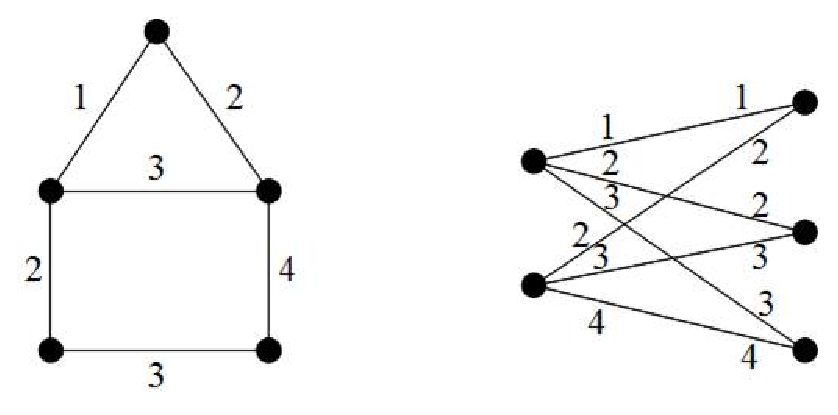
\includegraphics[width=20pc]{figures/W-bound-fig1.eps}\\
\caption{$3$ առավելագույն աստիճանով գրաֆներ, որոնք չունեն միջակայքային $3$-ներկում:}
\label{f1_cubic}
\end{center}
\end{figure}

Նկար \ref{f1_cubic}-ում պատկերված գրաֆները ցույց են տալիս, որ Թեորեմ \ref{t1_lower_matching_number}-ի ստորին գնահատականները հասանելի են: 

\begin{corollary}
\label{c1_lower_nopm} Եթե $G$ կապակցված մուլտիգրաֆը չունի կատարյալ զուգակցում և $G\in \mathfrak{N}$, ապա
\begin{center}
$w(G)\geq \max\{\Delta(G),2\delta(G)\}$:
\end{center}
\end{corollary}



Վերջապես, ապացուցենք Հետևանք \ref{c1_lower_nopm}-ի անալոգը կենտ մուլտիգրաֆների համար: $G$ մուլտիգրաֆը կանվանենք կենտ մուլտիգրաֆ, եթե $G$-ի բոլոր գագաթների աստիճանները կենտ են:

\begin{theorem}
\label{t1_lower_odd} Եթե $G$-ն կապակցված կենտ մուլտիգրաֆ է, $\vert
E(G)\vert-\frac{\vert V(G)\vert}{2}$ թիվը կենտ է և $G\in \mathfrak{N}$,
ապա
\begin{center}
$w(G)\geq \max\{\Delta(G),2\delta(G)\}$:
\end{center}
\end{theorem}
\begin{proof}[Ապացույց] Նշանակենք $\delta=\delta(G)$: Եթե $G$-ն չունի կատարյալ զուգակցում, ապա արդյունքը հետևում է Հետևանք \ref{c1_lower_nopm}-ից: Ենթադրենք $G$-ն ունի կատարյալ զուգակցում: Այժմ կատարենք հակասող ենթադրություն, դիցուք $G$-ն ունի $\alpha$ միջակայքային $t$-ներկում որևէ $t\leq 2\delta-1$ թվի համար: Քանի որ ցանկացած $v\in V(G)$, $1\leq \underline S\left(v,\alpha \right)\leq
\delta$, ստանում ենք, որ $\delta\in 
S_{\cap}\left(V(G),\alpha\right)$: Այստեղից հետևում է, որ $\delta$ գույնով ներկված կողերը $G$-ում կազմում են կատարյալ զուգակցում: Նշանակենք այդ կատարյալ զուգակցումը $M$-ով և դիտարկենք $G-M$ մուլտիգրաֆը: Սահմանենք $G-M$-ի $\beta$ ներկումը հետևյալ կերպ. ցանկացած $e\in E(G-M)$ կողի համար
\begin{center}
$\beta\left(e\right)=\left\{
\begin{tabular}{ll}
$\alpha(e)$, & երբ $1\leq \alpha(e)\leq \delta -1$,\\
$\alpha(e)-1$, & երբ $\delta+1\leq \alpha(e)\leq t$.\\
\end{tabular}%
\right.$
\end{center}

\begin{figure}[h]
\begin{center}
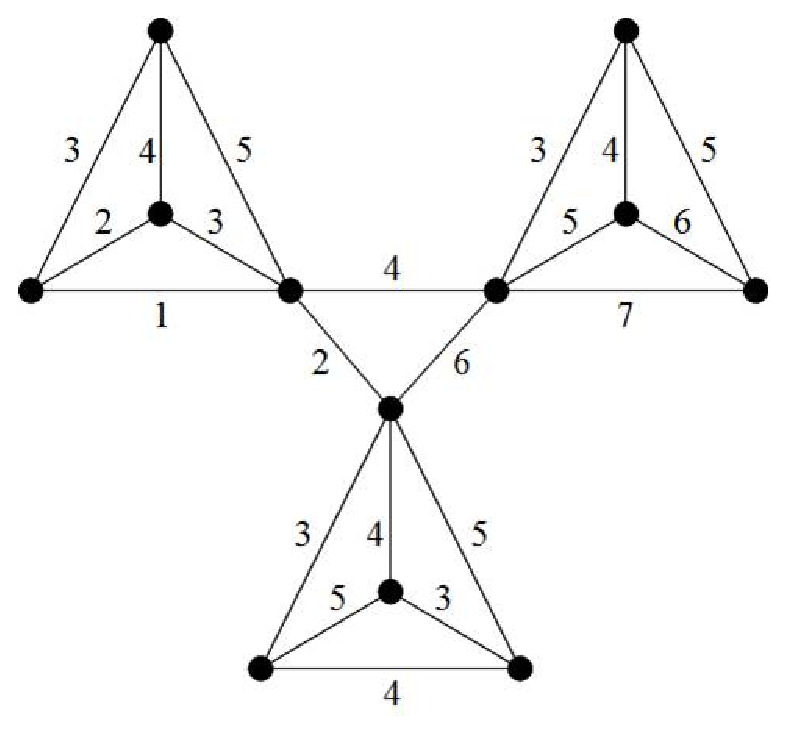
\includegraphics[width=20pc]{figures/W-bound-fig2.eps}\\
\caption{Միջակայքային ներկելի կապակցված գրաֆ $G$, որի բոլոր գագաթների աստիճանները կենտ են, $|E(G)|-\frac{|V(G)|}{2}=15$ և $w(G) \geq 6$:}
\label{f1_odd}
\end{center}
\end{figure}

Դժվար չէ տեսնել, որ $\beta$-ն $G-M$-ի միջակայքային $(t-1)$-ներկում է: Քանի որ $\vert E(G)\vert-\frac{\vert V(G)\vert}{2}$ կենտ է, ստանում ենք, որ $G-M$-ը զույգ մուլտիգրաֆ է կենտ թվով կողերով: Այստեղից հետևում է, որ $G-M$-ը ունի կենտ թվով կողեր պարունակող էյլերյան կապակցված բաղադրիչ, որը միջակայքային ներկելի է, ինչը հակասում է Հետևանք \ref{c1_eulerian}-ին:
\end{proof}


\subsection{Միջակայքային ներկման և հատուկ տիպի ֆակտորիզացիայի համարժեքությունը լրիվ գրաֆների համար}

Լրիվ գրաֆների միջակայքային ներկելիության խնդիրը ունի պարզ լուծում: $n$ գագաթանի լրիվ գրաֆը $(n-1)$-համասեռ է, իսկ մյուս կողմից հեշտ է տեսնել, որ $\chi'(K_n)=\Delta(K_n)$ այն և միայն այն դեպքում, երբ $n$-ը զույգ է: Ուստի, ըստ Թեորեմ \ref{t1_class1}-ի, լրիվ գրաֆը ունի միջակայքային ներկում այն և միայն այն դեպքում, երբ գագաթների քանակը զույգ է: Կենտ գագաթանի լրիվ գրաֆների նվազագույն դեֆիցիտով ներկումները մանրամասն հետազոտված են այս աշխատանքի \ref{s_wdef} պարագրաֆում:

Այս և հաջորդ պարագրաֆերում կուսումնասիրվեն զույգ գագաթանի լրիվ գրաֆների միջակայքային ներկումներում հանդիպող գույների քանակները: Նույն Թեորեմ \ref{t1_class1}-ից հետևում է, որ $w(K_{2n}) = 2n-1$ և կամայական $t$ բնական թվի համար, $w(K_{2n}) \leq t \leq W(K_{2n})$, $K_{2n}$ գրաֆը ունի միջակայքային $t$-ներկում: Սակայն $W(K_{2n})$ պարամետրը գտնելու խնդիրը մնում է բաց 1990 թվականից \cite{Kamalian1990}: Այս պարագրաֆում կառաջարկենք լրիվ գրաֆների միջակայքային ներկումներ կառուցելու նոր եղանակ, որի հիման վրա հաջորդ պարագրաֆում կստանանք $W(K_{2n})$-ի նոր գնահատականներ և որոշ ճշգրիտ արժեքներ:

$W(K_{2n})$-ի առաջին գնահատականը ստացվել է Քամալյանի կողմից \cite{Kamalian1990}.
\begin{theorem}
Ցանկացած $n\in \mathbb{N}$ թվի համար $W(K_{2n}) \geq 2n-1 + \left\lfloor \log_2(2n-1) \right\rfloor$:
\end{theorem}


Հետագայում Պետրոսյանին հաջողվել էր լավացնել այս գնահատականը \cite{Petrosyan2010}.
\begin{theorem}\label{tPetrosyan3n2}
Ցանկացած $n\in \mathbb{N}$ թվի համար $W(K_{2n}) \geq 3n-2$:
\end{theorem}

Նույն հոդվածում նա ցույց էր տվել, որ եթե ունենք որևէ լրիվ գրաֆի միջակայքային ներկում, ապա դրա հիման վրա կարելի է կառուցել երկու անգամ ավելի շատ գագաթներով լրիվ գրաֆի միջակայքային ներկում.

\begin{theorem}\label{tPetrosyan4n}
Կամայական $n\in \mathbb{N}$ թվի համար $W(K_{4n}) \geq 4n-1 + W(K_{2n})$:
\end{theorem}

Այս երկու արդյունքները միավորելով Պետրոսյանը ստացել էր $W(K_{2n})$-ի մինչ այժմ հայտնի լավագույն ստորին գնահատականը.
\begin{theorem}
\label{t2_complete_pq} Եթե $n=p2^{q}$, որտեղ $p$-ն կենտ է, իսկ $q \in \mathbb{Z}_{\geq 0}$, ապա
\begin{center}
$W\left(K_{2n}\right)\geq 4n-2-p-q$:
\end{center}
\end{theorem}

Նույն հոդվածում Պետրոսյանը ձևակերպել էր հիպոթեզ, ըստ որի այս ստորին գնահատականը հենց $W(K_{2n})$-ի ճշգրիտ արժեքն է: 
\begin{hypothesis}
\label{h1_complete_pq}
Եթե $n=p2^{q}$, որտեղ $p$-ն կենտ է, իսկ $q \in \mathbb{Z}_{\geq 0}$, ապա
\begin{center}
$W\left(K_{2n}\right) = 4n-2-p-q$:
\end{center}
\end{hypothesis}

Պետրոսյանին հաջողվել էր ցույց տալ, որ հիպոթեզը ճիշտ է, երբ $n \leq 4$: Արդեն $n=5$ դեպքում հիպոթեզը հերքվեց, $K_{10}$-ի $14$ գույներով ներկումը պատկերված է Նկ. \ref{t2_K10}-ում:

\begin{figure}[b!]
\centering
\includegraphics[width=0.74\textwidth]{figures/K_10-14.pdf}
\caption{$K_{10}$-ի միջակայքային $14$-ներկում: $sp(\alpha) = (1,2,1,1)$}
\label{t2_K10}
\end{figure}

$W(K_{2n})$-ի հայտնի լավագույն վերին գնահատականը հետևում է Թեորեմ \ref{t1_upper_2V-4}-ից.
\begin{center}
$W(K_{2n}) \leq 4n-4$, երբ $n \geq 2$:
\end{center}

2010-ին մեր կողմից առաջարկվեց հետևյալ հիպոթեզը.
\begin{hypothesis}
\label{h1_complete_log}
$W(K_{2n}) = 4n-2-\left \lfloor \log_2{n} \right \rfloor - \left \| n_2 \right \|$, որտեղ $\left \| n_2 \right \|$-ը $n$ թվի երկուական ներկայացման մեջ $1$-երի քանակն է:
\end{hypothesis}

Համակարգչային ծրագրի միջոցով հաջողվել էր կառուցել այս հիպոթեզին բավարարող ներկումներ $n \leq 14$-ի համար:
 
Լրիվ գրաֆի միջակայքային կողային ներկումների կառուցման նոր եղանակը նկարագրելու համար ներմուծենք մի շարք սահմանումներ և նշանակումներ:

$K_{2n}$ լրիվ գրաֆի գագաթները նշանակենք հետևյալ կերպ. $V(K_{2n}) = \{u_i, v_i : i=1,2,\ldots,n\}$: Գագաթների կամայական ֆիքսված $\mathbf{v} = \left(u_1,v_1, u_2,v_2, \ldots,u_n,v_n\right)$ համարակալման համար $H_{\mathbf{v}}^{[i,j]}$-ով, $i \leq j$, նշանակենք $K_{2n}$-ի $u_i, v_i, u_{i+1}, v_{i+1}, \ldots, u_j, v_j$ գագաթներով ծնված ենթագրաֆը: 

Դիցուք $\mathfrak{F} = \{F_1, F_2, \ldots, F_{2n-1}\}$ բազմությունը $K_{2n}$-ի $1$-ֆակտորիզացիա է: Ցանկացած $F\in \mathfrak{F}$ զուգակցման համար սահմանենք իր \textit{ձախ և աջ մասերը} գագաթների $\mathbf{v}$ համարակալման նկատմամբ:
\begin{align*}
l_{\mathbf{v}}^i(F) &= F \cap E\left(H_{\mathbf{v}}^{[1,i]}\right)\\
r_{\mathbf{v}}^i(F) &= F \cap E\left(H_{\mathbf{v}}^{[i+1,n]}\right)
\end{align*}

Եթե որևէ $i$ թվի համար, $1 \leq i \leq n-1$, $F = l_{\mathbf{v}}^i(F) \cup r_{\mathbf{v}}^i(F)$, ապա $F$-ը կոչվում է \textit{$i$-բաժանված} կատարյալ զուգակցում $\mathbf{v}$ համարակալման նկատմամբ: Այլ կերպ ասած, $F$-ի կողերը չեն հատում գագաթների $i$-րդ և $(i+1)$-րդ զույգերի միջև անցող ուղղահայաց ուղիղը ($F_1^1$-ը և $F_1^2$-ը Նկ. \ref{K_6factorization}-ում):

Դիցուք $\alpha$-ն $K_{2n}$-ի որևէ միջակայքային ներկում է: Կարող ենք գագաթները վերանվանել այնպես, որ բավարարվեն հետևյալ անհավասարությունները: 
\begin{center}
$\underline{S}(u_i, \alpha) \leq \underline{S}(v_i, \alpha) \leq \underline{S}(u_{i+1}, \alpha)\leq \underline{S}(v_{i+1}, \alpha)$, $i=1,2,\ldots,n-1$.
\end{center}
Այսպիսով, կամայական $\alpha$ ներկման համար գոյություն ունի գագաթների հատուկ համարակալում՝ $\mathbf{v}_\alpha = \left(u_1,v_1, u_2,v_2, \ldots,u_n,v_n\right)$, որի համար այս անհավասարությունները բավարարվում են: 

Այժմ ֆիքսենք $\mathbf{v}_\alpha$ համարակալումը և ուսումնասիրենք $\alpha$ ներկման որոշ հատկություններ: Նախ ցույց տանք, որ $u_i$ և $v_i$ գագաթների սպեկտրները նույնն են:

\begin{remark}
\label{spectrumIntersection}
$K_{2n}$-ի ցանկացած $\alpha$ միջակայքային կողային ներկման համար, $S_\cap\left(K_{2n}, \alpha\right) \neq \emptyset$: Հակառակ դեպքում դա կհակասեր Թեորեմ \ref{t1_upper_2V-3}-ի վերին գնահատականին:
\end{remark}

\begin{lemma}
Եթե $1 \leq i \leq n$, ապա $\underline{S}(u_i, \alpha) = \underline{S}(v_i, \alpha)$.
\end{lemma}
\begin{proof}[Ապացույց]
Պնդում \ref{spectrumIntersection}-ից հետևում է, որ եթե $\underline{S}(v_i, \alpha) - \underline{S}(u_{i}, \alpha) > 0$, ապա $\underline{S}(u_{i}, \alpha)$ գույնով ներկված կողերը կազմում են կատարյալ զուգակցում $K_{2n}\left[\{u_1,v_1,u_2,v_2,\ldots,u_i\}\right]$ ենթագրաֆում, ինչը հնարավոր չէ, քանի որ այն ունի կենտ թվով գագաթներ:
\end{proof}

Կամայական $\alpha$ ներկման համար սահմանենք իր \textit{շեղումների վեկտորը} հետևյալ կերպ.
\begin{center}
${\rm sh}(\alpha) = (b_1, b_2, \ldots, b_{n-1})$ \\
որտեղ $b_i = \underline{S}(u_{i+1}, \alpha) - \underline{S}(u_i, \alpha)$, $i=1,2,\ldots,n-1$
\end{center}

$B_i$-ով նշանակենք հետևյալ մասնակի գումարները. $B_0 = 0$ և $B_i = \sum\limits_{j=1}^{i}b_j$, $i=1,2,\ldots,n-1$:

$\alpha$ ներկման \textit{գումարային շեղումը} սահմանվում է հետևյալ կերպ.

\begin{center}
$|{\rm sh}(\alpha)| = B_{n-1} = \sum\limits_{i=1}^{n-1}b_i$
\end{center}

\begin{remark}
\label{totalShift}
Եթե $\alpha$-ն $K_{2n}$-ի միջակայքային $t$-ներկում է և ${\rm sh}(\alpha) = (b_1, b_2, \ldots, b_{n-1})$, ապա $t = 2n-1 + |{\rm sh}(\alpha)|$:
\end{remark}

\begin{remark}
\label{middleColors}
$K_{2n}$-ի կամայական $\alpha$ միջակայքային կողային ներկման համար բոլոր գագաթներում հանդիպող գույներն են. $S_\cap\left(K_{2n}, \alpha\right) = \left[\underline{S}(u_n, \alpha), \overline{S}(u_1, \alpha)\right] = \left[|{\rm sh}(\alpha)|+1, 2n-1\right] = \left\{|{\rm sh}(\alpha)|+j  : j=1,2,\ldots,2n-1-|{\rm sh}(\alpha)|\right\}$:
\end{remark}

Կամայական $i=1,2,\ldots,n-1$, թվի համար սահմանենք հետևյալ երկու գույների բազմությունները.
\begin{align*}
L_{\mathbf{v}_\alpha}^i(\alpha) &= \left\{
\begin{tabular}{ll}
$[\underline{S}(u_{i}, \alpha), \underline{S}(u_{i+1}, \alpha) - 1] 
=\{ B_{i-1} + j : j=1,2,\ldots,b_i \}$, &երբ $b_i>0$,\\
$\emptyset$, & երբ $b_i=0$,\\
\end{tabular}%
\right.\\
R_{\mathbf{v}_\alpha}^i(\alpha) &= \left\{
\begin{tabular}{ll}
$[\overline{S}(u_{i}, \alpha) + 1, \overline{S}(u_{i+1}, \alpha)] 
=\{ B_{i-1} + 2n-1 + j : j=1,2,\ldots,b_i \}$, & երբ $b_i>0$,\\
$\emptyset$, & երբ $b_i=0$:\\
\end{tabular}%
\right.
\end{align*}

\begin{remark}
\label{splittedColors}
Եթե $\alpha$-ն $K_{2n}$-ի միջակայքային $t$-ներկում է, և ${\rm sh}(\alpha) = (b_1, b_2, \ldots, b_{n-1})$, ապա
\begin{center}
\begin{tabular}{ll}
$L_{\mathbf{v}_\alpha}^i(\alpha) \subset S_\cap\left(H_{\mathbf{v}_\alpha}^{[1,i]},\alpha\right)$
&$L_{\mathbf{v}_\alpha}^i(\alpha) \cap S_\cup\left(H_{\mathbf{v}_\alpha}^{[i+1,n]},\alpha\right) = \emptyset$\\
$R_{\mathbf{v}_\alpha}^i(\alpha) \cap S_\cup\left(H_{\mathbf{v}_\alpha}^{[1,i]},\alpha\right) = \emptyset$ 
&$R_{\mathbf{v}_\alpha}^i(\alpha) \subset S_\cap\left(H_{\mathbf{v}_\alpha}^{[i+1,n]},\alpha\right)$
\end{tabular}
\end{center}
\end{remark}

$C_k(\alpha)$-ով նշանակենք $k$ գույնով ներկված կողերի բազմությունը. $C_k(\alpha) = \{e \in E(K_{2n}) : \alpha(e)=k\}$:

\begin{figure}[t!]
\centering
\includegraphics[width=0.7\textwidth]{figures/K_6factorization.pdf}
\caption{$K_6$-ի միջակայքային $7$-ներկումը և համապատասխան $1$-ֆակտորիզացիան՝ $\mathfrak{F}=\left\{F_1^1, F_1^2, F_1^0, F_2^0, F_3^0\right\}$}
\label{K_6factorization}
\end{figure}

\begin{lemma}[Համարժեքության լեմմա]\label{lEquiv}
Հետևյալ երկու պնդումները համարժեք են.
\begin{description}
\item{(ա)} գոյություն ունի $K_{2n}$-ի $\alpha$ միջակայքային կողային ներկում այնպես, որ ${\rm sh}(\alpha) = (b_1, b_2, \ldots b_{n-1})$,
\item{(բ)} գոյություն ունի գագաթների $\mathbf{v}$ համարակալում և $K_{2n}$-ի $\mathfrak{F} = 
\left\{ F^0_j : j=1,2,\ldots,2n-1-\sum\limits_{i=1}^{n-1}b_i \right\}
\cup
\bigcup\limits_{i=1}^{n-1}\left\{F^i_j : j=1,2,\ldots,b_i\right\}$ $1$-ֆակտորիզացիա այնպես, որ $F^i_j$-ն $i$-բաժանված է $\mathbf{v}$ համարակալման նկատմամբ, $i=1,2,\ldots,n-1$, $j=1,2,\ldots,b_i$, $b_i \in \mathbb{Z}_{\geq 0}$:
\end{description}
\end{lemma}

\begin{proof}[Ապացույց]
Ապացույցի ընթացքում $B_i$-ով կնշանակենք $\sum\limits_{j=1}^{i}b_j$ գումարը, $i=0,1,\ldots,n-1$:

\begin{description}
\item{(ա) $=>$ (բ)}. Դիցուք $\alpha$-ն $K_{2n}$-ի միջակայքային $t$-ներկում է, որի համար ${\rm sh}(\alpha) = (b_1, b_2, \ldots b_{n-1})$: Ֆիքսենք գագաթների $\mathbf{v}_\alpha$ համարակալումը և կառուցենք $K_{2n}$-ի $\mathfrak{F}$ $1$-ֆակտորիզացիան: 

Պնդում \ref{middleColors}-ի համաձայն գոյություն ունեն $2n-1-|{\rm sh}(\alpha)|$ գույներ, որոնք հանդիպում են բոլոր գագաթների սպեկտրներում: Ըստ սահմանման, $|{\rm sh}(\alpha)| = \sum\limits_{i=1}^{n-1}b_i$, ուստի կարող ենք վերցնել $F_j^0 = C_{|{\rm sh}(\alpha)|+j}(\alpha)$, որտեղ $j=1,2,\ldots,2n-1-|{\rm sh}(\alpha)|$:

Պնդում \ref{splittedColors}-ից հետևում է, որ ցանկացած $i=1,2,\ldots,n-1$, թվի համար գոյություն ունեն $|L_{\mathbf{v}_\alpha}^i(\alpha)|=b_i$ իրարից տարբեր գույներ, որոնք հանդիպում են միայն գագաթների առաջին $i$ զույգերի սպեկտրներում, և ևս $|R_{\mathbf{v}_\alpha}^i(\alpha)|=b_i$ իրարից տարբեր գույներ, որոնք հանդիպում են միայն մնացած $2n-2i$ գագաթների սպեկտներում: Վերցնենք $F^i_j = C_{B_{i-1} + j}(\alpha) \cup C_{B_{i-1} + 2n - 1 + j}(\alpha)$, կամայական $i=1,2,\ldots,n-1$ և $j=1,2,\ldots,b_i$ թվերի համար: Նկատենք, որ $L_{\mathbf{v}_\alpha}^i(\alpha) \cup R_{\mathbf{v}_\alpha}^i(\alpha)$ բազմության գույներով ներկված կողերը չեն հատում $i$-րդ և $(i+1)$-րդ գագաթների զույգերի միջև անցնող ուղղահայաց ուղիղը ($F_1^1$ և $F_1^2$ Նկ. \ref{K_6factorization}-ում), ուստի $F^i_j$-ն բոլոր թույլատրելի $j$-երի համար $i$-բաժանված կատարյալ զուգակցում է գագաթների $\mathbf{v}_\alpha$ համարակալման նկատմամբ:

\item{(բ) $=>$ (ա)}. Ենթադրենք $\mathfrak{F} = 
\left\{ F^0_j : j=1,2,\ldots,2n-1-|{\rm sh}(\alpha)| \right\}
\cup
\bigcup\limits_{i=1}^{n-1}\left\{F^i_j : j=1,2,\ldots,b_i\right\}$ $K_{2n}$-ի $1$-ֆակտորիզացիա է, ընդ որում $F_j^i$-ն $i$-բաժանված կատարյալ զուգակցում է գագաթների $\mathbf{v}=\left(u_1,v_1, u_2,v_2, \ldots,u_n,v_n\right)$ համարակալման նկատմամբ, $i=1,2,\ldots,n-1$, $j=1,2,\ldots,b_i$: Կառուցենք $K_{2n}$-ի $\alpha$ միջակայքային կողային ներկումը հետևյալ կերպ.

\begin{tabular}{lll}
$\alpha(e)=B_{i-1} + j$ & երբ $e \in l_{\mathbf{v}}^i(F_j^i)$ & $i=1,2,\ldots,n-1$, $j=1,2,\ldots,b_i$ \\
$\alpha(e)=B_{n-1} + j$ & երբ $e \in F_j^0$ & $j=1,2,\ldots,2n-1-B_{n-1}$\\
$\alpha(e)=B_{i-1} + 2n - 1 + j$ & երբ $e \in r_{\mathbf{v}}^i(F_j^i)$ & $i=1,2,\ldots,n-1$, $j=1,2,\ldots,b_i$
\end{tabular}

Այն փաստից, որ $F^i_j$-ն գագաթների $\mathbf{v}$ համարակալման նկատմամբ $i$-բաժանված կատարյալ զուգակցում է, հետևում է, որ $K_{2n}$-ի կամայական կող ստացել է որևէ գույն: Իրոք, $u_i$ (նաև $v_i$) գագաթը ծածկված է բոլոր $F_j^0$ զուգակցումներով, $j=1,2,\ldots,2n-1-B_{n-1}$, $F_j^{i'}$, զուգակցումների ձախ մասերով, $i'=i,i+1,\ldots,n-1$, և $F_j^{i'}$ զուգակցումների աջ մասերով, $i'=1,2,\ldots,i-1$, կամայական $j=1,2,\ldots,b_{i'}$ թվի համար: Ուստի գագաթների սպեկտրները կլինեն.
\begin{align*}
S(u_i, \alpha) = S(v_i, \alpha) &= \bigcup\limits_{i'=i}^{n-1}\{B_{i'-1} + j  : j=1,2,\ldots,b_{i'}\} \\
& \cup
\{B_{n-1} + j : j=1,2,\ldots,2n-1-B_{n-1}\} \\
& \cup
\bigcup\limits_{i'=1}^{i-1}\{B_{i'-1} + 2n-1 + j  : j=1,2,\ldots,b_{i'}\}\\
&= [B_{i-1}+1, B_{n-1}] \cup [B_{n-1}+1, 2n-1] \cup [2n, B_{i-1}+2n-1]\\
&= [B_{i-1}+1, B_{i-1}+2n-1]
\end{align*}

Սա ցույց է տալիս, որ $\alpha$-ն $K_{2n}$-ի  միջակայքային $(B_{n-1} + 2n-1)$-ներկում է: Լեմմայի ապացույցն ավարտելու համար անհրաժեշտ է ստուգել կառուցված $\alpha$ ներկման շեղումների վեկտորը: Նկատենք, որ կամայական $i=1,2,\ldots,n-1$, թվի համար ունենք, որ $\underline{S}(u_{i+1}, \alpha) - \underline{S}(u_{i}, \alpha) = B_{i}-B_{i-1} = b_i$: Սա նշանակում է, որ գագաթների $\mathbf{v}_\alpha$ համարակալումը համընկնում է $\mathbf{v}$ համարակալման հետ և ${\rm sh}(\alpha) = (b_1, b_2, \ldots, b_{n-1})$:
\end{description}

\end{proof}

\begin{remark}\label{splittedSameColor}
Համարժեքության լեմմայի ապացույցի առաջին մասում կառուցված $F_j^0$ զուգակցումների մի մասը ևս կարող են լինել բաժանված կատարյալ զուգակցումներ, սակայն նրանց թե՛ աջ և թե՛ ձախ մասերը $\alpha$ ներկման մեջ ունեն նույն գույնը: Օրինակ, երբ $|{\rm sh}(\alpha)|=0$, $F^0_{\alpha(u_1v_1)} = C_{\alpha(u_1v_1)}(\alpha)$ զուգակցումը $1$-բաժանված կատարյալ զուգակցում է գագաթների $\mathbf{v}_\alpha$ համարակալման նկատմամբ:
\end{remark}

\begin{corollary}\label{cEquiv}
Ցանկացած $n\in\mathbb{N}$-ի համար $K_{2n}$-ը ունի միջակայքային $t$-ներկում այն և միայն այն դեպքում, երբ այն ունի այնպիսի $1$-ֆակտորիզացիա, որտեղ առնվազն $t-2n+1$ կատարյալ զուգակցումներ բաժանված են:
\end{corollary}
\begin{proof}[Ապացույց]
Տրված միջակայքային $t$-ներկմանը համապատասխանող $1$-ֆակտորիզացիայի կառուցումը անմիջականորեն հետևում է Պնդում \ref{totalShift}-ից և Համարժեքության լեմմայից: Պնդում \ref{splittedSameColor}-ից հետևում է, որ ստացված $1$-ֆակտորիզացիայում բաժանված կատարյալ զուգակցումների թիվը կարող է մեծ լինել $t-2n+1$ թվից:

Եթե տրված է $K_{2n}$-ի $1$-ֆակտորիզացիա, որտեղ առնվազն $t-2n+1$ կատարյալ զուգակցումներ բաժանված են, կարող ենք դրանցից ընտրել որևէ $t-2n+1$-ը, ապա դրանցից յուրաքանչյուրի համար ընտրել որևէ $i$ թիվ, որի համար այն $i$-բաժանված է (միևնույն կատարյալ զուգակցումը կարող է միաժամանակ լինել և՛ $i$-բաժանված, և՛ $i'$-բաժանված տարբեր $i$ և $i'$ թվերի համար, ընտրությունը կրկին կամայական է) և կիրառել Համարժեքության լեմման: Այսպիսով, ստացված ներկումը կարող է միակը չլինել:
\end{proof}

Այս հետևանքը ցույց է տալիս, որ $K_{2n}$ գրաֆի մեծ թվով գույներով ներկում գտնելը համարժեք է մեծ թվով բաժանված կատարյալ զուգակցումներ պարունակող $1$-ֆակտորիզացիայի գտնելուն (գագաթների որևէ համարակալման նկատմամբ): Գագաթների ֆիքսված $\mathbf{v}$ համարակալման համար կարող ենք սահմանել բաժանված կատարյալ զուգակցումների առավելագույն թիվը ըստ $K_{2n}$-ի բոլոր $1$-ֆակտորիզացիաների: Լրիվ գրաֆի սիմետրիայի պատճառով այդ թիվը իրականում կախված չէ գագաթների $\mathbf{v}$ համարակալման ընտրությունից, ուստի այն կարող ենք նշանակել $\sigma_n$-ով:

\begin{theorem}[Համարժեքության թեորեմ]\label{tEquiv}
Ցանկացած $n\in \mathbb{N}$ թվի համար $W(K_{2n}) = 2n-1+\sigma_n$:
\end{theorem}


\subsection{Լրիվ գրաֆի միջակայքային ներկման առավելագույն գույների քանակի գնահատականներ}

\subsubsection{Ստորին գնահատականներ}

$W(K_{2n})$-ի համար նոր ստորին գնահատականներ ստանալու $K_{2n}$-ը տրոհենք երկու կողերով չհատվող կմախքային համասեռ ենթագրաֆների, կառուցենք հատուկ տիպի $1$-ֆակտորիզացիաներ ենթագրաֆներից յուրաքանչյուրի համար, ապա կիրառենք Համարժեքության լեմման այդ $1$-ֆակտորիզացիաների միավորման համար:

Ֆիքսենք $K_{2n}$-ի գագաթների որևէ համարակալում՝ $\mathbf{v} = \left(u_1,v_1, u_2,v_2, \ldots,u_n,v_n\right)$, և սահմանենք $K_{2n}$-ի երկու համասեռ կմախքային ենթագրաֆներ՝ $K_2 \square K_n$ և $K_2 \times K_n$ (Նկ. \ref{K_8products}).
\begin{align*}
&V(K_2 \square K_n) = V(K_2 \times K_n) = V(K_{2n})\\
&E(K_2 \square K_n) = \{u_iu_j : 1\leq i<j \leq n\} \cup \{u_iv_i : 1\leq i \leq n\} \cup \{v_iv_j : 1\leq i<j \leq n\}\\
&E(K_2 \times K_n) = \{u_iv_j : 1\leq i \neq j \leq n\}
\end{align*}


\begin{figure}[b!]
\centering
\includegraphics[width=0.43\textwidth]{figures/K_8products.pdf}
\caption{$K_8$-ի երկու համասեռ կմախքային ենթագրաֆներ}
\label{K_8products}
\end{figure}


Նկատենք, որ $E(K_{2n})=E(K_2 \square K_n)\cup E(K_2 \times K_n)$: Ֆիքսված $\mathbf{v} = \left(u_1,v_1, u_2,v_2, \ldots,u_n,v_n\right)$ համարակալման համար կառուցենք $K_2 \square K_n$ գրաֆի հատուկ $1$-ֆակտորիզացիա, որը կնշանակենք $\mathfrak{P}_n$-ով.

$\mathfrak{P}_n = \{P_0, P_1, \ldots, P_{n-1}\}$, որտեղ 
\begin{align*}
P_0 &= \left\{
\begin{tabular}{ll}
$\{u_ju_{n+1-j}, v_jv_{n+1-j} : j=1,2,\ldots,\frac{n}{2}\}$ 
& երբ $n$-ը զույգ է\\
$\{u_ju_{n+1-j}, v_jv_{n+1-j} : j=1,2,\ldots,\lfloor\frac{n}{2}\rfloor\}
\cup \{u_{\frac{n+1}{2}}v_{\frac{n+1}{2}}\}$, & երբ $n$-ը կենտ է\\
\end{tabular}%
\right.
\end{align*}

Բոլոր $i=1,2,\ldots,n-1$, թվերի համար սահմանենք $P_i = l_{\mathbf{v}}^i(P_i) \cup r_{\mathbf{v}}^i(P_i)$, որտեղ
\begin{align*}
l_{\mathbf{v}}^i(P_i) &= \left\{
\begin{tabular}{ll}
$\{u_ju_{i+1-j}, v_jv_{i+1-j} : j=1,2,\ldots,\frac{i}{2}\}$ 
& երբ $i$-ն զույգ է\\
$\{u_ju_{i+1-j}, v_jv_{i+1-j} : j=1,2,\ldots,\lfloor\frac{i}{2}\rfloor\}
\cup \{u_{\frac{i+1}{2}}v_{\frac{i+1}{2}}\}$, & երբ $i$-ն կենտ է\\
\end{tabular}%
\right.\\
r_{\mathbf{v}}^i(P_i) &= \left\{
\begin{tabular}{ll}
$\{u_{i+j}u_{n+1-j}, v_{i+j}v_{n+1-j} : j=1,2,\ldots,\frac{n-i}{2}\}$ 
& երբ $n-i$ զույգ է\\
$\{u_{i+j}u_{n+1-j}, v_{i+j}v_{n+1-j} : j=1,2,\ldots,\lfloor\frac{n-i}{2}\rfloor\}
\cup \{u_{\frac{n+i+1}{2}}v_{\frac{n+i+1}{2}}\}$, & երբ $n-i$ կենտ է\\
\end{tabular}%
\right.
\end{align*}

\begin{figure}[t!]
\centering
\includegraphics[width=0.7\textwidth]{figures/P_6.pdf}
\caption{$K_2 \square K_6$-ի $\mathfrak{P}_6$ $1$-ֆակտորիզացիան}
\label{P_6}
\end{figure}


Պարզ է, որ $P_i$-ն $i$-բաժանված կատարյալ զուգակցում է բոլոր $i=1,2,\ldots,n-1$ թվերի համար: Նկատենք, որ $K_2 \times K_n$-ը համասեռ երկկողմանի գրաֆ է, ուստի ըստ Քյոնիգի թեորեմի \cite{Konig1916} այն ունի $1$-ֆակտորիզացիա: Եթե $K_2 \times K_n$-ի $1$-ֆակտորիզացիայի բոլոր կատարյալ զուգակցումները համարենք չտրոհված զուգակցումներ և ավելացնենք $\mathfrak{P}_n$-ի կատարյալ զուգակցումները, ապա կստանանք, որ $\sigma_n \geq n-1$: Համարժեքության թեորեմից հետևում է, որ այս արդյունքը համարժեք է Թեորեմ \ref{tPetrosyan3n2}-ին: 

Այս ստորին գնահատականը լավացնելու համար փորձենք կառուցել $K_2 \times K_n$-ի ավելի լավ $1$-ֆակտորիզացիա:

\begin{lemma}\label{l35n3}
Եթե $n \geq 2$, ապա $\sigma_n \geq \lfloor 1.5n \rfloor - 2$:
\end{lemma}
\begin{proof}[Ապացույց]
Ֆիքսենք գագաթների $\mathbf{v} = \left(u_1,v_1,u_2,v_2,\ldots,u_n,v_n\right)$ համարակալումը և դիտարկենք երկու ծնված ենթագրաֆներ.
\begin{align*}
G_1 &= K_2 \times K_n\left[\left\{u_1,v_1,u_2,v_2,\ldots,u_{\lfloor\frac{n}{2}\rfloor},v_{\lfloor\frac{n}{2}\rfloor}\right\}\right]\\ 
G_2 &= K_2 \times K_n\left[\left\{u_{\lfloor\frac{n}{2}\rfloor + 1},v_{\lfloor\frac{n}{2}\rfloor + 1},
u_{\lfloor\frac{n}{2}\rfloor + 2},v_{\lfloor\frac{n}{2}\rfloor + 2},\ldots,u_n,v_n \right\}\right]
\end{align*}
Երկու ենթագրաֆերն էլ համասեռ են ու երկկողմանի, հետևաբար ըստ Քյոնիգի թեորեմի \cite{Konig1916} ունեն $1$-ֆակտորիզացիա: Դիցուք $G_1$-ի և $G_2$-ի $1$-ֆակտորիզացիաներն են համապատասխանաբար $F^l_1,F^l_2,\ldots,F^l_{\lfloor\frac{n}{2}\rfloor-1}$ և $F^r_1,F^r_2,\ldots,F^r_{\lceil\frac{n}{2}\rceil-1}$: Միավորելով այս զուգակցումների առաջին $\lfloor\frac{n}{2}\rfloor-1$ զույգերը, կստանանք $K_2 \times K_n$-ի $\lfloor\frac{n}{2}\rfloor$-բաժանված կատարյալ զուգակցումներ $\mathbf{v}$ համարակալման նկատմամբ.

\begin{center}
$F_i = F^l_i \cup F^r_i$, բոլոր $i=1,2,\ldots,\lfloor\frac{n}{2}\rfloor - 1$ թվերի համար:
\end{center}

Եթե $K_2 \times K_n$ գրաֆից հանենք $\bigcup\limits_{i=1}^{\lfloor\frac{n}{2}\rfloor-1}F_i$ կողերը, ստացված գրաֆը ևս համասեռ երկկողմանի է և ունի $1$-ֆակտորիզացիա, որը նշանակենք $\mathfrak{F}_0$-ով: Ստացվում է, որ $\mathfrak{F}_0 \cup \bigcup\limits_{i=1}^{\lfloor\frac{n}{2}\rfloor-1}F_i \cup \mathfrak{P}_n$ $K_{2n}$-ի $1$-ֆակտորիզացիա է: Բաժանված կատարյալ զուգակցումների քանակը $\lfloor\frac{n}{2}\rfloor - 1 + n - 1$ է: Ուստի ստանում ենք, որ $\sigma_n \geq \lfloor 1.5n \rfloor - 2$:
\end{proof}

Կիրառելով Համարժեքության թեորեմը՝ ստանում ենք հետևյալ ստորին գնահատականը.
\begin{theorem}
\label{t35n3}
Եթե $n \geq 2$, ապա $W(K_{2n}) \geq \lfloor 3.5n \rfloor - 3$:
\end{theorem}

Այս թեորեմից հետևում է, որ $W(K_{10}) \geq 14$, որը Հիպոթեզ \ref{h1_complete_pq}-ը հերքող ամենափոքր օրինակն է: Այսուհետ կքննարկենք այն դեպքը, երբ $n$-ը բաղադրյալ թիվ է:

\begin{lemma}\label{lComposite}
Ցանկացած $m,n \in\mathbb{N}$ թվերի համար $\sigma_{mn} \geq \sigma_m + \sigma_n + 2(m-1)(n-1)$:
\end{lemma}
\begin{proof}[Ապացույց]
Նշանակենք $K_{2mn}$, $K_{2n}$ և $K_{2m}$ գրաֆների գագաթների բազմությունը հետևյալ կերպ.
\begin{align*}
V(K_{2mn}) &= \left\{u_i^j,v_i^j : i=1,2,\ldots,n,\ j=1,2,\ldots,m\right\} \\
V(K_{2n}) &= \left\{\overline{u}_i,\overline{v}_i : i=1,2,\ldots,n \right\} \\ 
V(K_{2m}) &= \left\{\widetilde{u}^i,\widetilde{v}^i : i=1,2,\ldots,m \right\} 
\end{align*}


\begin{figure}[t!]
\centering
\includegraphics[width=0.39\textwidth]{figures/K_18-1.pdf}
\hspace{1cm}
\includegraphics[width=0.39\textwidth]{figures/K_18-2.pdf}
\caption{$K_{18}$-ի որոշ կատարյալ զուգակցումներ հիմնված $K_6$-ի $\overline{\mathfrak{F}}=\{N_1,N_2,N_1^0,N_2^0,N_3^0\}$, $K_6$-ի $\widetilde{\mathfrak{F}}=\{M_1,M_2,M_1^0,M_2^0,M_3^0\}$ և $K_2\square K_6$-ի $\mathfrak{P}_6=\{P_0,P_1,P_2,P_3,P_4,P_5\}$ $1$-ֆակտորիզացիաների վրա՝ Լեմմա \ref{lComposite}-ի միջոցով:}
\label{K_18matchings}
\end{figure}


Ֆիքսենք, համապատասխանաբար, $K_{2mn}$-ի, $K_{2n}$-ի և $K_{2m}$-ի գագաթների համարակալումները.
\begin{align*}
\mathbf{v} &= \left(
u^1_1,v^1_1,u^1_2,v^1_2, \ldots, u^1_n,v^1_n,
u^2_1,v^2_1,u^2_2,v^2_2, \ldots, u^2_n,v^2_n, \ldots, 
u^m_1,v^m_1,u^m_2,v^m_2, \ldots, u^m_n,v^m_n \right) \\
\overline{\mathbf{v}} &= \left(
\overline{u}_1,\overline{v}_1,\overline{u}_2,\overline{v}_2, \ldots, \overline{u}_n,\overline{v}_n\right)\\
\widetilde{\mathbf{v}} &= \left(
\widetilde{u}^1,\widetilde{v}^1,\widetilde{u}^2,\widetilde{v}^2, \ldots, \widetilde{u}^m,\widetilde{v}^m\right)
\end{align*}

Դիցուք $\overline{\mathfrak{F}} = \{ N_1,N_2,\ldots,N_{\sigma_n},N^0_1,N^0_2,\ldots, N^0_{2n-1-\sigma_n} \}$ հանդիսանում է $K_{2n}$-ի $1$-ֆակտորիզացիա, որտեղ $N_i$-ն բաժանված կատարյալ զուգակցումներ է, երբ $i=1,2,\ldots,\sigma_n$: Դիցուք $\widetilde{\mathfrak{F}} = \{ M_1,M_2,\ldots,M_{\sigma_m},M^0_1,M^0_2,\ldots, M^0_{2m-1-\sigma_m} \}$ հանդիսանում է $K_{2m}$-ի $1$-ֆակտորիզացիա, որտեղ $M_i$-ն բաժանված կատարյալ զուգակցում է, երբ $i=1,2,\ldots,\sigma_m$: 

Մենք նաև կօգտագործենք $K_2 \square K_{2m}$ գրաֆը, $\left\{w_i,z_i : i=1,2,\ldots,2m\right\}$ գագաթների բազմությամբ, $\mathbf{w} = \left( w_1,z_1,w_2,z_2,\ldots,w_{2m},z_{2m} \right)$ գագաթների համարակալմամբ և իր $\mathfrak{P}_{2m} = \{P_0,P_1,\ldots,P_{2m-1} \}$ $1$-ֆակտորիզացիայով, որը սահմանվում է ինչպես այս պարագրաֆի սկզբում: $K_2 \square K_{2m}[\{w_{2k-1},w_{2k},z_{2k-1},z_{2k}\}]$ ենթագրաֆը կանվանենք $K_2 \square K_{2m}$-ի $k$-րդ բջիջ, որտեղ $1 \leq k \leq m$:

Ապացույցի ընթացքում միշտ կհամարենք, որ $x,y \in \{u,v\}$, $1 \leq s,t \leq n$ և $1 \leq p,q \leq m$:

Դիցուք $\overline{\varphi}$-ն արտապատկերում է $K_{2mn}$-ի կողերը $K_{2n}$-ի կողերի վրա: Ցանկացած $x^p_sy^q_t \in E(K_{2mn})$ կողի համար, որտեղ $x_s \neq y_t$, սահմանենք $\overline{\varphi}(x^p_sy^q_t)=\overline{x}_s\overline{y}_t$: Այնուհետև սահմանենք $\widetilde{\varphi}$ արտապատկերումը $K_{2mn}$-ի մնացած կողերից $K_{2m}$-ի կողերի մեջ: Ցանկացած $x^p_sx^q_s \in E(K_{2mn})$ կողի համար սահմանենք $\widetilde{\varphi}( x^p_sx^q_s ) = \widetilde{x}^p\widetilde{x}^q$: Նկատենք, որ $\overline{\varphi}^{-1}(\overline{e})$ նախապատկերները բոլոր $\overline{e} \in E(K_{2n})$ կողերի համար և $\widetilde{\varphi}^{-1}(\widetilde{x}^p\widetilde{x}^q)$ նախապատկերները բոլոր $\widetilde{x}^p\widetilde{x}^q \in E(K_{2m})$ կողերի համար զույգ առ զույգ տարբեր են, իսկ նրանց միավորումը ծածկում է ամբողջ $E(K_{2mn})$ բազմությունը: $E(K_{2mn})$ բազմությունը տրոհենք երեք չհատվող մասերի հետևյալ կերպ.
\begin{align*}
E(K_{2mn}) &= E^1 \cup E^2 \cup E^3 \text{, որտեղ} \\
E^1 &= \bigcup\limits_{i=1}^{\sigma_n}{\bigcup\limits_{\overline{e} \in N_i}{\overline{\varphi}^{-1}(\overline{e})}} \\
E^2 &= \bigcup\limits_{i=2}^{2n-1-\sigma_n}\bigcup\limits_{\overline{e} \in N^0_i}{\overline{\varphi}^{-1}(\overline{e})} \\
E^3 &= \bigcup\limits_{\overline{e} \in N^0_1}{\overline{\varphi}^{-1}(\overline{e})} \cup \bigcup\limits_{\widetilde{x}^p\widetilde{x}^q \in E(K_{2m})}{\widetilde{\varphi}^{-1}(\widetilde{x}^p\widetilde{x}^q)}
\end{align*}

$K_{2mn}$-ի կառուցվելիք $1$-ֆակտորիզացիան կնշանակենք $\mathfrak{F}$-ով և այն նույնպես բաղկացած կլինի երեք մասերից:

\begin{center}
$\mathfrak{F} = \mathfrak{F}^1 \cup \mathfrak{F}^2 \cup \mathfrak{F}^3$
\end{center}

$\mathfrak{F}^k$ կատարյալ զուգակցումների բազմությունը ծածկելու է $E^k$ կողերի բազմությունը, որտեղ $k=1,2,3$: Նկ. \ref{K_18matchings}-ում պատկերված են երեք մասերից յուրաքանչյուրը ծածկող կատարյալ զուգակցումները, երբ $m=n=3$:

$E^1$ բազմությունը բաղկացած է $K_{2n}$-ի բաժանված կատարյալ զուգակցումների նախապատկերներից: Այն ծածկելու համար կամայական $N_i \in \overline{\mathfrak{F}}$ բաժանված կատարյալ զուգակցման համար, $i=1,2,\ldots,\sigma_n$, և կամայական կենտ ինդեքսով $P_{2j+1} \in \mathfrak{P}_{2m}$ կատարյալ զուգակցման համար, $j=0,1,\ldots,m-1$, կառուցենք $\mathfrak{F}^1$-ի մեկ կատարյալ զուգակցում. 
\begin{align*}
F^1_{i,j} = &F^1_{i,j,1} \cup F^1_{i,j,2} \cup F^1_{i,j,3} \cup F^1_{i,j,4}\text{, որտեղ }\\
F^1_{i,j,1} = &\bigcup\limits_{\substack{w_{2k-1}z_{2k-1} \in P_{2j+1} \\ 1 \leq k \leq m}}
\left\{x_s^ky_t^k : \overline{x}_s\overline{y}_t \in l(N_i)\right\} \\
F^1_{i,j,2} = &\bigcup\limits_{\substack{w_{2k}z_{2k} \in P_{2j+1} \\ 1 \leq k \leq m}}
\left\{x_s^ky_t^k : \overline{x}_s\overline{y}_t \in r(N_i)\right\} \\
F^1_{i,j,3} = &\bigcup\limits_{\substack{w_{2k-1}w_{2l-1} \in P_{2j+1} \\ 1 \leq k < l \leq m}}
\left\{x_s^ky_t^l, y_t^kx_s^l : \overline{x}_s\overline{y}_t \in l(N_i)\right\} \\
F^1_{i,j,4} = &\bigcup\limits_{\substack{w_{2k}w_{2l} \in P_{2j+1} \\ 1 \leq k < l \leq m}}
\left\{x_s^ky_t^l, y_t^kx_s^l : \overline{x}_s\overline{y}_t \in r(N_i)\right\}\\
\mathfrak{F}^1 = &\left\{F^1_{i,j} : i=1,2,\ldots,\sigma_n,\ j=0,1,\ldots,m-1\right\}
\end{align*}

$F^1_{i,j,1}$-ը և $F^1_{i,j,2}$-ը կառուցելու համար դիտարկում ենք $P_{2j+1}$ կատարյալ զուգակցման ուղղաձիգ կողերը: Եթե որևէ $k$ թվի համար, $k$-րդ բջջի ձախ (աջ) կողմի ուղղաձիգ կողը պատկանում է $P_{2j+1}$-ին, ապա $K_{2mn}$-ի $k$-րդ $K_{2n}$-ի կրկնօրինակում $l(N_i)$-ի ($r(N_i)$-ի) բոլոր կողերի նախապատկերները ավելացնում ենք $F^1_{i,j,1}$-ին ($F^1_{i,j,2}$-ին): Ցանկացած $P_{2j+1}$ զուգակցում պարունակում է ճիշտ երկու ուղղաձիգ կող ($w_{j+1}z_{j+1}$ և $w_{j+m+1}z_{j+m+1}$): Երբ $m$-ը կենտ է, այդ երկու ուղղաձիգ կողերից մեկը գտնվում է իր բջջի ձախ մասում, իսկ մյուսը՝ իր բջջի աջ մասում: Երբ $m$-ը զույգ է, ապա եթե $j$-ն կենտ է (զույգ է), երկու ուղղաձիգ կողերն էլ գտնվում են իրենց բջիջների աջ (ձախ) կողմում: Այսպիսով, $F^1_{i,j,1}$-ի և $F^1_{i,j,2}$-ի կողերի քանակները կարելի է հաշվարկել հետևյալ կերպ.
\begin{align*}
|F^1_{i,j,1}| = &|l(N_i)|\left( (m \bmod 2)\cdot 1 + (1 - m \bmod 2)\cdot 2(1 - j \bmod 2) \right) \\
|F^1_{i,j,2}| = &|r(N_i)|\left( (m \bmod 2)\cdot 1 + (1 - m \bmod 2)\cdot 2(j \bmod 2) \right) 
\end{align*}

$F^1_{i,j,3}$-ը ($F^1_{i,j,4}$-ը) կառուցելու համար դիտարկում ենք $P_{2j+1}$-ի այն կողերը, որոնք միացնում են երկու տարբեր բջիջների ձախ (աջ) մասերը: Երբ $m$-ը կենտ է, գոյություն ունեն այդպիսի $\frac{m-1}{2}$ կողեր: Երբ $m$-ը զույգ է, ապա այդպիսի կողերի թիվը $\frac{m}{2} - (1 - j \bmod 2)$ է ($F^1_{i,j,4}$-ի դեպքում՝ $\frac{m}{2} - (j \bmod 2)$): $k$-րդ և $l$-րդ բջիջները ($k<l$) միացնող այդպիսի կողերից յուրաքանչյուրի համար $F^1_{i,j,3}$-ին ($F^1_{i,j,4}$-ին) ավելացնում ենք $l(N_i)$-ի ($r(N_i)$-ի) բոլոր այն նախապատկերները, որոնք միացնում են $K_{2mn}$-ում $K_{2n}$-ի $k$-րդ և $l$-րդ կրկնօրինակները: Նկատենք, որ $P_{2j+1}$-ի ամեն մի ֆիքսված կողին համապատասխանող $l(N_i)$-ի ($r(N_i)$-ի) յուրաքանչյուր կող ունի ճիշտ երկու նախապատկեր $F^1_{i,j,3}$-ում ($F^1_{i,j,4}$-ում). Ուստի ունենք հետևյալը.
\begin{align*}
|F^1_{i,j,3}| = &2|l(N_i)|\left( (m \bmod 2)\cdot \frac{m-1}{2} + (1 - m \bmod 2)\cdot \left(\frac{m}{2} - (1 - j \bmod 2)\right) \right) \\
|F^1_{i,j,4}| = &2|r(N_i)|\left( (m \bmod 2)\cdot \frac{m-1}{2} + (1 - m \bmod 2)\cdot \left(\frac{m}{2} - (j \bmod 2)\right) \right)
\end{align*}

$F^1_{i,j}$-ի կառուցումից հետևում է, որ այն զուգակցում է $K_{2mn}$-ում: Որպեսզի հիմնավորենք, որ այն նաև կատարյալ զուգացկում է, պետք է ցույց տալ, որ այն ունի ճիշտ $mn$ թվով կողեր: 
\begin{align*}
|F^1_{i,j}| = &|F^1_{i,j,1}| + |F^1_{i,j,2}| + |F^1_{i,j,3}| + |F^1_{i,j,4}| = \\
 = &|l(N_i)|\left(
 	(m \bmod 2)( 1 + m - 1) + 
    (1 - m \bmod 2)\left( 
    	2(1- j \bmod 2) + m - 2(1 - j\bmod 2) 
	\right)
\right) + \\
 + &|r(N_i)|\left(
 	(m \bmod 2)( 1 + m - 1) + 
    (1 - m \bmod 2)\left(
    	2(j \bmod 2) + m - 2(j\bmod 2)
    \right)
\right) \\
 = &\left(|l(N_i)| + |r(N_i)|\right)\left((m \bmod 2)\cdot m +  (1 - m \bmod 2)\cdot m \right) = nm
\end{align*}

$F^1_{i,j}$ և $F^1_{i',j'}$ զուգակցումները չեն հատվում, երբ $i \ne i'$ կամ $j \ne j'$, քանի որ նրանց կողերը համապատասխանում են կամ $K_{2n}$-ի տարբեր կողերի, կամ $K_2 \square K_{2m}$-ի տարբեր կողերի: Նաև նկատենք, որ եթե $N_i$-ն $r$-բաժանված կատարյալ զուգակցում է $\overline{\mathbf{v}}$ համարակալման նկատմամբ, ապա $F^1_{i,j}$-ը $(jn+r)$-բաժանված կատարյալ զուգակցում է $\mathbf{v}$ համարակալման նկատմամբ, բոլոր $i=1,2,\ldots,\sigma_n$ և $j=0,1,\ldots,m-1$ թվերի համար:

$E^2$ բազմությունը բաղկացած է բոլոր չբաժանված կատարյալ զուգակցումների նախապատկերներից, բացի մեկ չբաժանված կատարյալ զուգակցումից: Այն ծածկելու համար կամայական $N^0_i \in \overline{\mathfrak{F}}$ չբաժանված կատարյալ զուգակցման համար, բացի $N^0_1$-ից (այս բացառության ընտրությունը կամայական է) և կամայական զույգ ինդեքսով $P_{2j} \in \mathfrak{P}_{2m}$ կատարյալ զուգակցման համար կառուցենք $\mathfrak{F}^2$-ի մեկ կատարյալ զուգակցում:
\begin{align*}
F^2_{i,j} = &F^2_{i,j,1} \cup F^2_{i,j,2}\text{, որտեղ }\\
F^2_{i,j,1} = &\bigcup\limits_{\substack{w_{2k-1}w_{2k} \in P_{2j} \\ 1 \leq k \leq m}}
\left\{x_s^ky_t^k : \overline{x}_s\overline{y}_t \in N^0_i\right\} \\
F^2_{i,j,2} = &\bigcup\limits_{\substack{w_{2k-1}w_{2l} \in P_{2j} \\ 1 \leq k < l \leq m}}
\left\{x_s^ky_t^l, y_t^kx_s^l : \overline{x}_s\overline{y}_t \in N^0_i\right\}\\
\mathfrak{F}^2 = &\{F^2_{i,j} : i=2,3,\ldots,2n-1-\sigma_n,\ j=0,1,\ldots,m-1\}
\end{align*}
$P_{2j}$ զուգակցումները ունեն միայն հորիզոնական կողեր: Մեզ հետաքրքրում են այն կողերը, որոնք միացնում են որևէ բջջի ձախ մասը որևէ բջջի (նույն կամ տարբեր) աջ մասի հետ: Եթե կողի երկու ծայրակետերն էլ պատկանում են միևնույն $k$-րդ բջջին, ապա $N_i^0$-ի բոլոր կողերի այն նախապատկերները, որոնք $K_{2mn}$-ում պատկանում են $K_{2n}$-ի $k$-րդ կրկնօրինակին, ավելացնում ենք $F^2_{i,j,1}$ բազմությանը: $P_{2j}$-ում այդպիսի կողերի քանակը $1$ է, եթե $m$-ը կենտ է, և $2(j \bmod 2)$ է, եթե $m$-ը զույգ է: Ուստի, ունենք.
\begin{align*}
|F^2_{i,j,1}| = &n\left( (m \bmod 2)\cdot 1 + (1 - m \bmod 2)\cdot 2(j \bmod 2) \right)
\end{align*}
Եթե $P_{2j}$-ի կողը միացնում է $k$-րդ և $l$-րդ բջիջները ($k < l$), ապա $N_i^0$-ի բոլոր կողերի այն նախապատկերները, որոնք միացնում են $K_{2mn}$-ում $K_{2n}$-ի $k$-րդ և $l$-րդ կրկնօրինակների գագաթները, ավելացնում ենք $F^2_{i,j,2}$ բազմությանը: $P_{2j}$-ում այդպիսի կողերի քանակը $\frac{m-1}{2}$ է, եթե $m$-ը կենտ է, և $\frac{m}{2} - (j \bmod 2)$ է, եթե $m$-ը զույգ է: Ուստի.
\begin{align*}
|F^2_{i,j,2}| = &2n\left( (m \bmod 2)\cdot \frac{m-1}{2} + (1 - m \bmod 2)\cdot \left(\frac{m}{2} - (j \bmod 2)\right) \right) \\
|F^2_{i,j}| = &|F^2_{i,j,1}| + |F^2_{i,j,2}| =\\
= &n\left(
	(m \bmod 2)(1+m-1) + 
    (1 - m \bmod 2)(2(j \bmod 2) + m - 2(j \bmod 2))
\right) =\\
= &n\left(
	(m \bmod 2) \cdot m + 
    (1 - m \bmod 2) \cdot m
\right) = nm
\end{align*}

Ինչպես $\mathfrak{F}^1$-ի զուգակցումների դեպքում, $F^2_{i,j}$ և $F^2_{i',j'}$ զուգակցումները նույնպես չեն հատվում, երբ $i \ne i'$ կամ $j \ne j'$: Նկատենք, որ կամայական $i=2,3,\ldots,2n-1-\sigma_n$ թվի համար, $F^2_{i,j}$-ն $jn$-բաժանված կատարյալ զուգակցում է $\mathbf{v}$ համարակալման նկատմամբ երբ $j=1,2,\ldots,m-1$, իսկ երբ $j=0$, այն բաժանված կատարյալ զուգակցում չէ:

$E^3$ բազմությունը պարունակում է $K_{2n}$-ի $N^0_1$ չբաժանված կատարյալ զուգակցման բոլոր կողերի նախապատկերները և $K_{2m}[\{\widetilde{u}^1,\widetilde{u}^2,\ldots,\widetilde{u}^m\}] \cup K_{2m}[\{\widetilde{v}^1,\widetilde{v}^2,\ldots,\widetilde{v}^m\}]$ ենթագրաֆի բոլոր կողերի նախապատկերները: $K_{2m}$-ի կողերի նախապատկերները կազմում են թվով $2n$ իրար հետ չհատվող, $m$ գագաթանի լրիվ գրաֆներ՝ $K_{2mn}\left[\{x_s^1,x_s^2,\ldots,x_s^m\}\right]$, կամայական $\overline{x}_s \in V(K_{2n})$ գագաթի համար: Կամայական $\overline{x}_s\overline{y}_t \in N^0_1$ կողի համար, իր նախապատկերը և իր երկու $\overline{x}_s$ և $\overline{y}_t$ ծայրակետերին համապատասխանող $K_{m}$ ենթագրաֆները կազմում են $K_{2mn}\left[\{x_s^1,y_t^1,x_s^2,y_t^2,\ldots,x_s^m,y_t^m\}\right]$ ենթագրաֆը, որը իզոմորֆ է $K_{2m}$-ին: Այսինքն, $E^3$ բազմությունը կազմված է $K_{2m}$-ի թվով $n$ չհատվող կրկնօրինակներից: Կամայական $M \in \widetilde{\mathfrak{F}}$ կատարյալ զուգակցման համար կառուցում ենք $K_{2mn}$-ում մեկ կատարյալ զուգակցում միավորելով $E^3$-ում իր $n$ չհատվող կրկնօրինակները: 
\begin{align*}
F^3_{i} = &
\bigcup\limits_{\substack{\overline{x}_s\overline{y}_t \in N^0_1}}
\left\{ 
\{x_s^{p}x_s^{q} : \widetilde{u}^{p}\widetilde{u}^{q} \in M_i\} 
\cup 
\{x_s^{p}y_t^{q} : \widetilde{u}^{p}\widetilde{v}^{q} \in M_i\} 
\cup
\{y_t^{p}y_t^{q} : \widetilde{v}^{p}\widetilde{v}^{q} \in M_i\} 
\right\}\\
F'^3_{i} = &
\bigcup\limits_{\substack{\overline{x}_s\overline{y}_t \in N^0_1}}
\left\{ 
\{x_s^{p}x_s^{q} : \widetilde{u}^{p}\widetilde{u}^{q} \in M^0_i\} 
\cup 
\{x_s^{p}y_t^{q} : \widetilde{u}^{p}\widetilde{v}^{q} \in M^0_i\} 
\cup
\{y_t^{p}y_t^{q} : \widetilde{v}^{p}\widetilde{v}^{q} \in M^0_i\} 
\right\}\\
\mathfrak{F}^3 = &\left\{F^3_{i} : i=1,2,\ldots,\sigma_m\right\} \cup \left\{F'^3_{i} : i=1,2,\ldots,2m-1-\sigma_m\right\}
\end{align*}
$F^3_i$ և $F'^3_i$ զուգակցումները զույգ առ զույգ չեն հատվում և յուրաքանչյուրը բաղկացած է $mn$ կողերից: Նկատենք, որ եթե $M_i$-ն $r$-բաժանված կատարյալ զուգակցում է $\widetilde{\mathbf{v}}$ համարակալման նկատմամբ, ապա $F^3_i$-ն, $i=1,2,\ldots,\sigma_m$, $rn$-բաժանված կատարյալ զուգակցում է $\mathbf{v}$ համարակալման նկատմամբ: Իսկ $F'^3_i$, $i=1,2,\ldots,2m-1-\sigma_m$, կատարյալ զուգակցումները բաժանված չեն:

$\mathfrak{F}$ բազմության մեջ կատարյալ զուգակցումների թիվը $m\sigma_n + m(2n-2-\sigma_n) + 2m-1 = 2mn-1$ է: Այս կատարյալ զուգակցումներից բաժանված են միայն $m\sigma_n + (m-1)(2n-2-\sigma_n) + \sigma_m = \sigma_m+\sigma_n+2(m-1)(n-1)$ հատը: Ապացույցն ավարտված է:
\end{proof}

Կիրառելով Համարժեքության թեորեմը ստանում ենք հետևյալ ստորին գնահատականը, որն ընդհանրացնում է Թեորեմ \ref{tPetrosyan4n}-ը.
\begin{theorem}
\label{tComposite}
Ցանկացած $m,n \in\mathbb{N}$ թվերի համար $W(K_{2mn}) \geq W(K_{2m}) + W(K_{2n}) + 4(m-1)(n-1) - 1$:
\end{theorem}

Հայտնի է, որ $W(K_6) = 7$ և $W(K_{10}) \geq 14$: Վերոնշյալ թեորեմից հետևում է, որ $W(K_{30}) \geq 52$, ինչը հերքում է Հիպոթեզ \ref{h1_complete_log}-ը, ըստ որի $W(K_{30})=51$: Ինչպես կտեսնենք այս պարագրաֆի վերջում, սա հիպոթեզը հերքող ամենափոքր օրինակը չէ:

\begin{theorem}
\label{t1_lower}
Եթե $n=\prod\limits_{i=1}^{\pi(n)}p_i^{\alpha_i}$, որտեղ $p_i$-ն $i$-րդ պարզ թիվն է, $\pi(n)$-ը՝ $n$-ը չգերազանցող պարզ թվերի քանակը, իսկ $\alpha_i \in \mathbb{Z}_{\geq 0}$, ապա
\begin{center}
$W(K_{2n}) \geq 4n - 3 - \sum\limits_{i=1}^{\pi(n)}{\alpha_i\left(4p_i-3-W(K_{2p_i})\right)}$:
\end{center}
\end{theorem}
\begin{proof}[Ապացույց]
$d_m$-ով նշանակենք $W(K_{2m}) - (4m - 3)$ տարբերությունը: Թեորեմ \ref{tComposite}-ը պնդում է, որ $d_{mk} \geq d_m + d_k$: Մաթեմատիկական ինդուկցիայի եղանակով ստանում ենք, որ $d_n \geq \sum_{i=1}^{\pi(n)}{\alpha_i d_{p_i}}$: Ապացույցը կավարտվի, եթե $d_{p_i}$-ի փոխարեն տեղադրենք իր արժեքը:
\end{proof}

Մինչև $W(K_{2n})$-ի վերին գնահատականներին անցնելը ցույց տանք, որ վերը շարադրված թեորեմները թույլ են տալիս գնահատել նաև $W(G)$ պարամետրը, երբ $G$-ն ստացվում է լրիվ գրաֆից մեկ կատարյալ զուգակցում հանելով:

\begin{theorem}
\label{t1-complete-minus-matching}
Եթե $G$ գրաֆը ստացվում է $K_{2n}$ լրիվ գրաֆից մեկ կատարյալ զուգակցում հանելով, ապա $W(G) \geq W(K_{2n})-1$:
\end{theorem}
\begin{proof}[Ապացույց]
Դիցուք $\alpha$-ն $K_{2n}$-ի որևէ միջակայքային $W(G)$-ներկում է, որի համար ${\rm sh}(\alpha) = (b_1, b_2, \ldots b_{n-1})$: Ըստ Պնդում \ref{spectrumIntersection}-ի $K_{2n}$-ում գոյություն ունի $F$ կատարյալ զուգակցում, որի բոլոր կողերը ներկված են միևնույն $c$ գույնով: $K_{2n}$ գրաֆից հանենք $F$ զուգակցումը և ստացված գրաֆի համար կառուցենք $\beta$ ներկումը հետևյալ կերպ.
\begin{align*}
    \beta(e) &= \left\{
\begin{tabular}{ll}
$\alpha(e)$, & երբ $\alpha(e) < c$\\
$\alpha(e) - 1$, & երբ $\alpha(e) > c$
\end{tabular}%
\right.
\end{align*}
Կամայական $v \in V(K_{2n}-F)$ գագաթի սպեկտրը կլինի $S(v,\beta) = \left[\underline{S}(v,\alpha), \overline{S}(v,\alpha)-1\right]$: Հետևաբար, $\beta$-ն $K_{2n}-F$ գրաֆի միջակայքային $\left(W(K_{2n})-1\right)$-ներկում է և $W(K_{2n} - F) \geq W(K_{2n})-1$: 
\end{proof}



\subsubsection{Վերին գնահատականներ}


\begin{figure}[t!]
\centering
\includegraphics[width=\textwidth]{figures/K_16-26.pdf}
\caption{$K_{16}$-ի միջակայքային $26$-ներկում: ${\rm sh}(\alpha) = (1,2,1,3,1,2,1)$}
\label{f2_K16}
\end{figure}



Դիցուք $\alpha$-ն $K_{2n}$-ի կամայական միջակայքային կողային ներկում է, $n \in \mathbb{N}$, իսկ $\mathbf{v}_\alpha = \left(u_1,v_1, u_2,v_2, \ldots,u_n,v_n\right)$ ներկմանը համապատասխանող գագաթների համարակալումն է: Դիցուք $\alpha$-ի շեղման վեկտորն է ${\rm sh}(\alpha) = (b_1,b_2,\ldots,b_{n-1})$: Համարժեքության լեմմայից հետևում է, որ գոյություն ունի $K_{2n}$-ի $\mathfrak{F} = 
\left\{ F^0_j : j=1,2,\ldots,2n-1-\sum\limits_{i=1}^{n-1}b_i \right\}
\cup
\bigcup\limits_{i=1}^{n-1}\left\{F^i_j : j=1,2,\ldots,b_i\right\}$ 1-ֆակտորիզացիա այնպես, որ $F^i_j$-ն $i$-բաժանված է $\mathbf{v_\alpha}$ համարակալման նկատմամբ, $i=1,2,\ldots,n-1$, $j=1,2,\ldots,b_i$: Այս բաժնի բոլոր այն ապացույցներում, որտեղ կունենանք լրիվ գրաֆի $\alpha$ միջակայքային ներկում, կենթադրենք, որ տրված է նաև գագաթների համապատասխան $\mathbf{v}_{\alpha}$ համարակալումը և $\mathfrak{F}$ 1-ֆակտորիզացիան:

$W(K_{2n})$-ի վերին գնահատականները լավացնելու համար մեզ պետք կգան մի շարք լեմմաներ:

\begin{lemma}
\label{lReverse}
Եթե $K_{2n}$-ի որ և $\alpha$ միջակայքային կողային ներկման շեղման վեկտորը ${\rm sh}(\alpha) = (b_1,b_2,\ldots, b_{n-1})$ է, ապա գոյություն ունի $K_{2n}$-ի $\beta$ միջակայքային կողային ներկում այնպես, որ ${\rm sh}(\beta) = (b_{n-1}, b_{n-2}, \ldots, b_1)$:
\end{lemma}
\begin{proof}[Ապացույց]
Նկատենք, որ եթե որևէ $F \in \mathfrak{F}$ $i$-բաժանված է $\mathbf{v}_\alpha$ համարակալման նկատմամբ, ապա այն կլինի $(n-i)$-բաժանված $\mathbf{v}'_\alpha = \left(u_n,v_n,u_{n-1},v_{n-1},\ldots,u_1,v_1\right)$ համարակալման նկատմամբ: 
Կիրառենք Համարժեքության լեմման $\mathfrak{F}$-ից $\mathbf{v}'_\alpha$ համարակալման նկատմամբ $\beta$ ներկումը կառուցելու համար: Շեղումների վեկտորը կլինի $(b_{n-1}, b_{n-2}, \ldots, b_1)$:
\end{proof}

\begin{lemma}
\label{lLessColors}
Եթե $K_{2n}$-ի որևէ $\alpha$ միջակայքային կողային ներկման համար ${\rm sh}(\alpha) = (b_1,b_2,\ldots, b_{n-1})$, որտեղ $b_i > 0$ որևէ $i \in [1,n-1]$ թվի համար, ապա գոյություն ունի $K_{2n}$-ի $\beta$ միջակայքային կողային ներկում այնպես, որ ${\rm sh}(\beta) = (b_1, b_2, \ldots, b_{i-1}, b_{i}-1, b_{i+1}, \ldots, b_{n-1})$:
\end{lemma}
\begin{proof}[Ապացույց]
$b_i > 0$ պայմանից հետևում է, որ գոյություն ունի $F_{b_i}^i \in \mathfrak{F}$ կատարյալ զուգակցում, որը $i$-բաժանված է $\mathbf{v}_\alpha$ համարակալման նկատմամբ: Կառուցենք $\beta$ ներկումը կիրառելով Համարժեքության լեմման $\mathfrak{F}$ 1-ֆակտորիզացիայի նկատմամբ, համարելով $F_{b_i}^i$ զուգակցումը չբաժանված (կարող ենք վերանվանել այն $F^0_{2n-|{\rm sh}(\alpha)|}$):
\end{proof}


\begin{lemma}
\label{l2k1}
Եթե $K_{2n}$-ի որևէ $\alpha$ միջակայքային կողային ներկման համար ${\rm sh}(\alpha) = (b_1,b_2,\ldots, b_{n-1})$, ապա
\begin{center}
$\sum\limits_{i=1}^{k}{b_i} \leq 2k-1$, որտեղ $k=1,2,\ldots,n-1$:
\end{center}
\end{lemma}

\begin{proof}[Ապացույց]
Համարժեքության լեմմայի ապացույցի համաձայն $F^i_j$ կատարյալ զուգակցումների ձախ մասերը ծածկում են $u_1$ գագաթը (ինչպես նաև $v_1$-ը), $i=1,2,\ldots,k$, $j=1,2,\ldots,b_i$: Ավելին, 
\begin{center}
$\bigcup\limits_{i=1}^{k}
\bigcup\limits_{j=1}^{b_i}
{l^i_{\mathbf{v}_\alpha}\left(F^i_j\right)} 
\subset E\left(H_{\mathbf{v}_\alpha}^{[1,k]}\right)$
\end{center}
Ապացույցն ավարտելու համար նկատենք, որ $F^i_j$ կատարյալ զուգակցումների քանակը $\sum\limits_{i=1}^{k}{b_i}$ է, իսկ $u_1$ (կամ $v_1$) գագաթի աստիճանը $H_{\mathbf{v}_\alpha}^{[1,k]}$ ենթագրաֆում $2k-1$ է:
\end{proof}

$(b_1,b_2,\ldots,b_k)$ վեկտորը կանվանենք \textit{հագեցած}, եթե $\sum\limits_{i=1}^{k}{b_i} = 2k-1$:

\begin{corollary}
\label{c2n4}
Եթե $\alpha$-ն $K_{2n}$-ի միջակայքային կողային ներկում է, $n\geq 3$, ապա  
$|{\rm sh}(\alpha)| \leq 2n-4$:
\end{corollary}

\begin{proof}[Ապացույց]
Դիցուք ${\rm sh}(\alpha) = (b_1,b_2,\ldots, b_{n-1})$: Լեմմա \ref{l2k1}-ից հետևում է, որ $\sum\limits_{i=1}^{n-2}{b_i} \leq 2n-5$: Նույն լեմմայից Լեմմա \ref{lReverse}-ի հետ համատեղ բխում է, որ $b_{n-1} \leq 1$: Ապացույցը կավարտենք գումարելով այս երկու անհավասարությունները:
\end{proof}

\begin{lemma}
\label{lAfterSaturated}
Եթե $K_{2n}$-ի որևԷ $\alpha$ միջակայքային կողային ներկման համար ${\rm sh}(\alpha) = (b_1,b_2,\ldots, b_{n-1})$, և $(b_1,b_2,\ldots,b_k)$ վեկտորը հագեցած է որևէ $k \in [2,n-2]$ թվի համար, ապա $b_{k+1} \leq 1$:
\end{lemma}

\begin{proof}[Ապացույց]
Լեմմա \ref{l2k1}-ից հետևում է, որ $b_{k+1} \leq 2$: Ապացույցն ավարտելու համար անհրաժեշտ է ցույց տալ, որ $b_{k+1} \neq 2$: Ենթադրենք հակառակը՝ $b_{k+1} = 2$: $(b_1,b_2,\ldots,b_k)$ վեկտորը հագեցած է, ուստի Լեմմա \ref{l2k1}-ի ապացույցից բխում է, որ $u_1x_i$ և $v_1x_i$ կողերը, $x \in \{u,v\}$, $i=2,3,\ldots,k$, պատկանում են $F^i_j$ կատարյալ զուգակցումներին, $i=1,2,\ldots,k$, $j=1,2,\ldots,b_i$: Նմանապես, $u_1u_{k+1}$, $u_1v_{k+1}$, $v_1u_{k+1}$ և $v_1v_{k+1}$ կողերը պետք է ծածկված լինեն $F^{k+1}_1$-ով և $F^{k+1}_2$-ով:

Այժմ դիտարկենք $u_2$ գագաթը: Այն ծածկված է $F^i_j$ կատարյալ զուգակցումների ձախ մասերով, $i=2,3,\ldots,k$, $j=1,2,\ldots,b_i$: Բոլոր այս զուգակցումները միասին ծածկում են $H_{\mathbf{v}_\alpha}^{[1,k]}$ ենթագրաֆում $u_2$-ին կից բոլոր կողերը, բացի $2k-1 - \sum\limits_{i=2}^{k}{b_i} = b_1$ կողերից: Լեմմա \ref{l2k1}-ից բխում է, որ $b_1 \leq 1$, ուստի չծածկված մնում է առավելագույնը մեկ կող: $u_2$ գագաթը պետք է ծածկված լինի նաև $F^{k+1}_1$ և $F^{k+1}_2$ կատարյալ զուգակցումների ձախ մասերով: $u_2u_{k+1}$ և $u_2v_{k+1}$ կողերը չեն կարող օգտագործվել, քանի որ $u_{k+1}$ և $v_{k+1}$ արդեն ծածկված են $F^{k+1}_1$-ով և $F^{k+1}_2$-ով: Հետևաբար, այս երկու զուգակցումների մնում է առավելագույնը մեկ կող, ինչը հակասություն է:
\end{proof}


\begin{corollary}
\label{c2n5}
Եթե $\alpha$-ն $K_{2n}$-ի միջակայքային ներկում է և $n\geq 5$, ապա  
$|{\rm sh}(\alpha)| \leq 2n-5$:
\end{corollary}

\begin{proof}[Ապացույց]
Դիցուք ${\rm sh}(\alpha) = (b_1,b_2,\ldots, b_{n-1})$: Լեմմա \ref{l2k1}-ից հետևում է, որ $\sum\limits_{i=1}^{n-3}{b_i} \leq 2n-7$: Դիտարկենք երկու դեպք.
\begin{description}
\item{Դեպք 1.} $\sum\limits_{i=1}^{n-3}{b_i} = 2n-7$: Լեմմա \ref{lAfterSaturated}-ից բխում է, որ $b_{n-2} \leq 1$: Լեմմաներ \ref{lReverse} և \ref{l2k1}-ից հետևում է, որ $b_{n-1} \leq 1$: Գումարելով այս անհավասարությունները կստանանք պահանջված գնահատականը:
\item{Դեպք 2.} $\sum\limits_{i=1}^{n-3}{b_i} \leq 2n-8$: Լեմմաներ \ref{lReverse}-ից և \ref{l2k1}-ից հետևում է, որ $b_{n-2} + b_{n-1} \leq 3$: Գումարելով այս անհասավարությունները կավարտենք ապացույցը:
\end{description}
\end{proof}


\begin{lemma}
\label{lBeforeSaturated}
Եթե $K_{2n}$-ի որևէ $\alpha$ միջակայքային կողային ներկման համար ${\rm sh}(\alpha) = (b_1,b_2,\ldots, b_{n-1})$, և $(b_1,b_2,\ldots,b_k)$ վեկտորը հագեցած է որևէ $k \in [3,n-1]$ թվի համար, ապա $b_{k} \geq 3$:
\end{lemma}

\begin{proof}[Ապացույց]
Ենթադրենք հակառակը՝ $b_k \leq 2$: Եթե $b_k=2$, ապա $(b_1,b_2,\ldots,b_{k-1})$ վեկտորը ևս հագեցած է, ինչը բերում է հակասության Լեմմա \ref{lAfterSaturated}-ի հետ: Եթե $b_k \leq 1$, ապա ունենք, որ $\sum\limits_{i=1}^{k-1}{b_i} \geq 2k-2$, ինչը հակասում է Լեմմա \ref{l2k1}-ին:
\end{proof}



\begin{lemma}
\label{lEdgeCount}
Եթե $K_{2n}$-ի որևէ $\alpha$ միջակայքային կողային ներկման համար ${\rm sh}(\alpha) = (b_1,b_2,\ldots, b_{n-1})$, և $k \in [2,n-2]$, ապա
\begin{center}
$k(2k-1) \geq \sum\limits_{i=1}^{k}{ib_i} + \sum\limits_{i=k+1}^{\min\{2k-1,n-1\}}{(2k-i)b_i}$:
\end{center}
\end{lemma}
\begin{proof}[Ապացույց]
Դիտարկենք $H_{\mathbf{v}_\alpha}^{[1,k]}$ ենթագրաֆը: Այս ենթագրաֆում կողերի քանակը $k(2k-1)$ է: $F^i_j$ կատարյալ զուգակցումներից յուրաքանչյուրի ձախ մասը, $i=1,2,\ldots,k$, $j=1,2,\ldots,b_i$, բաղկացած է $i$ կողերից, և բոլորն էլ պատկանում են $H_{\mathbf{v}_\alpha}^{[1,k]}$ ենթագրաֆին: Այսպիսի կողերի քանակն է $\sum\limits_{i=1}^{k}{ib_i}$:

Այժմ ֆիքսենք որևէ $i \in [k+1,r]$, որտեղ $r$-ով նշանակել ենք $\min\{2k-1,n-1\}$-ը: $F_j^i$ կատարյալ զուգակցումներից յուրաքանչյուրի ձախ մասը, $j=1,2,\ldots,b_i$, բաղկացած է $i$ կողերից: Դրանցից առավելագույնը $(2i-2k)$-ը կարող են միացնել $H_{\mathbf{v}_\alpha}^{[1,k]}$-ի որևէ գագաթ $H_{\mathbf{v}_\alpha}^{[k+1,i]}$-ի որևէ գագաթի հետ: Ուստի առնվազն $2k-i$ կողեր պատկանում են $H_{\mathbf{v}_\alpha}^{[1,k]}$ ենթագրաֆին: Այդպիսի կողերի քանակը առնվազն $\sum\limits_{i=k+1}^{r}{(2k-i)b_i}$ է:
\end{proof}

Լեմմա \ref{lEdgeCount}-ից հետևում է, որ եթե որևէ ֆիքսված $k_0$-ի համար գոյություն ունեն մեծ թվով $i$-բաժանված կատարյալ զուգակցումներ, որտեղ $i \leq k_0$, ապա չեն կարող գոյություն ունենալ մեծ թվով $i'$-բաժանված կատարյալ զուգակցումներ, որտեղ $k_0 < i' < \min\{2k_0-1,n-1\}$: Այս լեմման օգտագործելու համար հարկավոր է $\sum\limits_{i=1}^{k}{ib_i}$ գումարը գնահատել ներքևից:

Կամայական $k\in \mathbb{N}$ և $r \in \mathbb{Z}_{\geq 0}$ թվերի համար սահմանենք հետևյալը.
\begin{align*}
&T_k = \left\{\left(b_1,b_2,\ldots,b_k\right) : \exists K_{2n}\text{-ի }\alpha \text{միջակայքային ներկում},\ n>k,\ {\rm sh}(\alpha)=(b_1,b_2,\ldots,b_{n-1})\right\} \\
&m(k,r) = \min\limits_{(b_1,b_2,\ldots,b_{k}) \in T_k}\left\{\sum\limits_{i=1}^{k}{ib_i} : \sum\limits_{i=1}^{k}{b_i}=r\right\}
\end{align*}
Նկատենք, որ $m(k,r)$-ը սահմանված չէ բոլոր $(k,r)$ զույգերի համար: Օրինակ, Լեմմա \ref{l2k1}-ից հետևում է, որ գոյություն չունեն $K_{2n}$-ի այնպիսի միջակայքային ներկումներ, որոնց համար $\sum\limits_{i=1}^{k}{b_i}=r$, երբ $r \geq 2k$: Ակնհայտ է, որ $m(1,1)=1$ և $m(k,0)=0$, որտեղ $k \in \mathbb{N}$:

\begin{remark}
$m(k,r)$-ը հաշվելու համար, $k>1$, $r>1$, բավական է վերցնել մինիմումը ըստ բոլոր այն $(b_1,b_2,\ldots,b_k) \in T_k$ վեկտորների, որոնց համար $\sum\limits_{i=1}^{k-1}{ib_i} = m(k-1,r-b_k)$:
\end{remark}


\begin{table}[t!]
\centering
\newcolumntype{C}{>{\centering\arraybackslash}X}%

\begin{tabularx}{0.8\textwidth}{c||C|C|C|C|}
\backslashbox{$r$}{$k$} & $1$ & $2$ & $3$ & $4$ \\ \hline\hline
$0$
& \begin{tabular}{c}$0$ \\ $(0)$ \end{tabular} 
& \begin{tabular}{c}$0$ \\ $(0,0)$ \end{tabular} 
& \begin{tabular}{c}$0$ \\ $(0,0,0)$ \end{tabular}  
& \begin{tabular}{c}$0$ \\ $(0,0,0,0)$ \end{tabular} \\ \hline

$1$ 
& \begin{tabular}{c}$1$ \\ $(1)$ \end{tabular} 
& \begin{tabular}{c}$1$ \\ $(1,0)$ \end{tabular} 
& \begin{tabular}{c}$1$ \\ $(1,0,0)$ \end{tabular} 
& \begin{tabular}{c}$1$ \\ $(1,0,0,0)$ \end{tabular} \\ \hline

$2$
&
& \begin{tabular}{c}$3$ \\ $(1,1)$ \end{tabular}  
& \begin{tabular}{c}$3$ \\ $(1,1,0)$ \end{tabular}  
& \begin{tabular}{c}$3$ \\ $(1,1,0,0)$ \end{tabular} \\ \hline

$3$
&
& \begin{tabular}{c}$5$ \\ $(1,2)$ \end{tabular}  
& \begin{tabular}{c}$5$ \\ $(1,2,0)$ \end{tabular} 
& \begin{tabular}{c}$5$ \\ $(1,2,0,0)$ \end{tabular} \\ \hline 


$4$
&
&
& \begin{tabular}{c}$8$ \\ $(1,2,1)$ \end{tabular} 
& \begin{tabular}{c}$8$ \\ $(1,2,1,0)$ \end{tabular} \\ \hline

$5$
&
&
& \begin{tabular}{c}$12$ \\ $(1,1,3)$ \end{tabular} 
& \begin{tabular}{c}$12$ \\ $(1,2,1,1)$ \end{tabular} \\ \hline

$6$
&
&
&  
& \begin{tabular}{c}$16$ \\ $(1,2,1,2)$ \end{tabular} \\ \hline

$7$
&
&
&  
& \begin{tabular}{c}$20$ \\ $(1,2,1,3)$ \end{tabular} \\ \hline
\end{tabularx}

\caption{
	$m(k,r)$-ի արժեքները: Յուրաքանչյուր վանդակի առաջին տողում գրված է $m(k,r)$-ի արժեքը: Երկրորդ տողում նշված է որևէ $(b_1,b_2,\ldots,b_k) \in T_k$ վեկտոր, որի համար $\sum\limits_{i=1}^{k}{ib_i} = m(k,r)$:
}
\label{tableMkr}
\end{table}

Աղյուսակ \ref{tableMkr}-ում թվարկված են $m(k,r)$-ի արժեքները, երբ $k\leq 4$ և $r \leq 7$: Օրինակ, $m(3,5)$-ը հաշվարկված է հետևյալ կերպ: Ըստ վերը նշված պնդման, $T_3$-ում թույլատրելի թեկնածու վեկտորներն են $(1,2,2)$-ը, $(1,1,3)$-ը, $(1,0,4)$-ը և $(0,0,5)$-ը: Լեմմա \ref{lAfterSaturated}-ից հետևում է, որ $(1,2,2) \notin T_3$: $K_{12}$-ի Նկ. \ref{fK12}-ում ներկայացված ներկումը ցույց է տալիս, որ $(1,1,3) \in T_3$: Մյուս կողմից, $b_1 + 2b_2 + 3b_3$ գումարը ավելի մեծ մյուս երկու թեկնածու վեկտորների համար, ուստի $m(3,5) = 12$: Նմանապես կարելի է ցույց տալ, որ $m(4,7)=20$, որտեղ մինիմումը հասանելի է $(1,2,1,3)$ վեկտորի համար, որը միանշանակ պատկանում է $T_4$ բազմությանը, ինչպես ցույց է տալիս $K_{22}$-ի Նկ. \ref{fK22}-ում պատկերված ներկումը: Լեմմա \ref{lLessColors}-ը կիրառելով այս երկու ներկումների համար կարող ենք ապացուցել, որ Աղյուսակ \ref{tableMkr}-ում նշված բոլոր վեկտորները պատկանում են համապատասխան $T_k$ բազմություններին:


\begin{figure}
\centering
\includegraphics[width=0.7\textwidth]{figures/K_12-16.pdf}
\caption{$K_{12}$-ի միջակայքային $16$-ներկումը $(1,1,3,0,0)$ շեղման վեկտորով:}
\label{fK12}
\end{figure}


\begin{lemma}
\label{l2n6}
Եթե $\alpha$-ն $K_{2n}$-ի միջակայքային կողային ներկում է և $n\geq 9$, ապա  
$|{\rm sh}(\alpha)| \leq 2n-6$:
\end{lemma}
\begin{proof}[Ապացույց]
Ենթադրենք հակառակը՝ $|{\rm sh}(\alpha)| \geq 2n-5$: Լեմմաներ \ref{lReverse}-ից և \ref{l2k1}-ից հետևում է, որ $\sum\limits_{i=5}^{n-1}{b_i} \leq 2n-11$: Դիտարկենք երեք դեպքեր:
\begin{description}
\item{Դեպք 1.} $\sum\limits_{i=5}^{n-1}{b_i} = 2n-11$: Լեմմաներ \ref{lReverse}-ից, \ref{lBeforeSaturated}-ից և \ref{lAfterSaturated}-ից հետևում է, որ $b_{5} \geq 3$ և $b_{4} \leq 1$: Կիրառենք Լեմմա \ref{l2k1}-ը՝ տեղադրելով $k=3$, և ցույց տանք, որ $b_{1} + b_{2} + b_{3} = 5$ և $b_{4}=1$: Ապա կիրառենք Լեմմա \ref{lEdgeCount}-ը՝ տեղադրելով $k=3$: Անհավասարության ձախ մասը հավասար է $15$-ի: Աջ կողմում ունենք $\sum\limits_{i=1}^{3}{ib_i} \geq m(3,5)=12$ և $\sum\limits_{i=4}^{5}{(6-i)b_i} \geq 5$: Այս անհավասարությունները հակասում են Լեմմա \ref{lEdgeCount}-ին:

\item{Դեպք 2.} $\sum\limits_{i=5}^{n-1}{b_i} = 2n-12$: Լեմմա \ref{l2k1}-ից բխում է, որ $(b_1,b_2,b_3,b_4)$ վեկտորը հագեցած է: Լեմմա \ref{lAfterSaturated}-ից հետևում է, որ $b_5 \leq 1$: Հետևաբար, $(b_{n-1},b_{n-2},\ldots,b_6)$ վեկտորը հագեցած է և $b_5=1$: Լեմմա \ref{lBeforeSaturated}-ից բխում է, որ $b_6 \geq 3$: Այժմ կիրառենք Լեմմա \ref{lEdgeCount}-ը՝ տեղադրելով $k=4$: Անհավասարության ձախ մասը հավասար է $28$-ի: Աջ մասում ունենք, որ $\sum\limits_{i=1}^{4}{ib_i} \geq m(4,7)=20$ և $\sum\limits_{i=5}^{7}{(8-i)b_i} \geq 9$: Այս անհավասարությունները հակասում են Լեմմա \ref{lEdgeCount}-ին:

\item{Դեպք 3.} $\sum\limits_{i=5}^{n-1}{b_i} \leq 2n-13$: Լեմմա \ref{l2k1}-ից հետևում է, որ $\sum\limits_{i=1}^{4}{b_i} \leq 7$: Գումարելով այս երկու անհավասարուըյունները ստանում ենք հակասություն:
\end{description}
\end{proof}

\begin{figure}
\centering
\includegraphics[width=\textwidth]{figures/K_22-37.pdf}
\caption{$K_{22}$-ի միջակայքային $37$-ներկում $(1,2,1,3,1,1,3,1,2,1)$ շեղման վեկտորով:}
\label{fK22}
\end{figure}


Հետևանքներ \ref{c2n4}-ից, \ref{c2n5}-ից, Լեմմա \ref{l2n6}-ից և Պնդում \ref{totalShift}-ից հետևում է $W(K_{2n})$-ի հետևյալ վերին գնահատականը:

\begin{theorem}
\label{tUpper}
Դիցուք $n \geq 3$:
\begin{center}
$W(K_{2n}) \leq \left\{
\begin{tabular}{ll}
$4n-5$, & երբ $n \geq 3$,\\
$4n-6$, & երբ $n \geq 5$,\\
$4n-7$, & երբ $n \geq 9$:\\
\end{tabular}
\right.$
\end{center}
\end{theorem}

Ստացված վերին գնահատականները թույլ են տալիս որոշել $W(K_{2n})$ պարամետրի ճշգրիտ արժեքները որոշ փոքր $n$-երի համար: Այդ արժեքները իրենց հերթին թույլ են տալիս լավացնել $W(K_{2n})$-ի ստորին գնահատականը, քանի որ Թեորեմ \ref{t1_lower}-ում ստացված գնահատականը կախված է $W(K_{2p})$ պարամետրի արժեքներից, որտեղ $p$-ն պարզ թիվ է: $p=2$ և $p=3$ դեպքերի համար $W(K_{2p})$-ի ճշգրիտ արժեքները հայտնի էին \cite{Petrosyan2010}-ից: $p=5$ դեպքում Թեորեմ \ref{t35n3}-ի ստորին գնահատականը համընկնում է Թեորեմ \ref{tUpper}-ի վերին գնահատականի հետ: $p=7$ դեպքը կլուծվի հաջորդ լեմմայում: Վերջապես, $p=11$ դեպքում Թեորեմ \ref{tUpper}-ի վերին գնահատականը հասանելի է $K_{22}$-ի միջակայքային $37$-ներկման միջոցով, որը պատկերված է Նկ. \ref{fK22}-ում: Այս ներկումը նաև հերքում է Հիպոթեզ \ref{h1_complete_log}-ը, ըստ որի $W(K_{22})=36$:

\begin{lemma}
\label{lK14}
$W(K_{14}) = 21$:
\end{lemma}
\begin{proof}[Ապացույց]
Թեորեմ \ref{tUpper}-ից հետևում է, որ $W(K_{14}) \leq 22$: Բավական է ցույց տալ, որ $K_{14}$-ը չունի միջակայքային կողային ներկում $22$ գույներով: Ենթադրենք հակառակը՝ գոյություն ունի $K_{14}$-ի $\alpha$ միջակայքային $22$-ներկում:

Դիտարկենք ներկման շեղման վեկտորը՝ ${\rm sh}(\alpha)=(b_1,b_2,b_3,b_4,b_5,b_6)$: Պնդում \ref{totalShift}-ից հետևում է, որ $\sum\limits_{i=1}^{6}{b_i}=9$: Լեմմա \ref{l2k1}-ից հետևում է, որ թե՛ առաջին և թե՛ վերջին եռյակի գումարը չի կարող գերազանցել $5$-ը: Առանց ընդհանրությունը խախտելու կարող ենք համարել, որ $b_1+b_2+b_3=5$ և $b_4+b_5+b_6=4$: Լեմմա \ref{lAfterSaturated}-ից բխում է, որ $b_4 \leq 1$: Լեմմաներ \ref{lReverse}-ից և \ref{l2k1}-ից հետևում է, որ $b_5+b_6=3$ և $b_4=1$: Ուստի $b_5 \geq 2$:

Այժմ ստուգենք Լեմմա \ref{lEdgeCount}-ի անհավասարությունը, երբ $k=3$: Ձախ մասը հավասար է $15$-ի: Աջ մասում ունենք, որ $\sum\limits_{i=1}^{3}{ib_i} \geq m(3,5) = 12$, $\sum\limits_{i=4}^{5}{(6-i)b_i} \geq 4$: Գումարելով այս անհավասարությունները ստանում ենք հակասություն:
\end{proof}

Լավագույն ստորին գնահատականը, որը հաջողվել է ստանալ, հետևյալն է: 

\begin{theorem}
\label{t1-complete-W-lower-best}
Եթե $n = \prod\limits_{i=1}^{\pi(n)}{p_i^{\alpha_i}}$, որտեղ $p_i$-ն $i$-րդ պարզ թիվն է, $\pi(n)$-ը՝ $n$-ը չգերազանցող պարզ թվերի քանակը, իսկ $\alpha_i \in \mathbb{Z}_{\geq 0}$, ապա
\begin{center}
$W(K_{2n}) \geq 4n - 3 - A_n$,
\end{center}
որտեղ $A_n = \alpha_1 + 2\alpha_2 + 3\alpha_3 + 4\alpha_4 + 4\alpha_5 + \frac{1}{2}\sum\limits_{i=6}^{\pi(n)}{\alpha_i(p_i+1)}$:
\end{theorem}
\begin{proof}[Ապացույց]
Թեորեմն ապացուցելու համար վերցնենք Թեորեմ \ref{t1_lower}-ի ստորին գնահատականը, տեղադրենք $W(K_{2p_i})$-ի ճշգրիտ արժեքները առաջին հինգ պարզ թվերի համար, իսկ $W(K_{2p_i})$ թվերը, $i\geq 6$, գնահատելու համար կիրառենք Թեորեմ \ref{t35n3}-ը՝ հաշվի առնելով, որ բացի $2$-ից բոլոր պարզ թվերը կենտ են:
\end{proof}

Այս Թեորեմից և Թեորեմ \ref{t1_regular}-ից ստանում ենք հետևյալ արդյունքը.
\begin{corollary}
Եթե $n = \prod\limits_{i=1}^{\pi(n)}{p_i^{\alpha_i}}$, որտեղ $p_i$-ն $i$-րդ պարզ թիվն է, $\alpha_i \in \mathbb{Z}_{\geq 0}$, $\pi(n)$-ը՝ $n$-ը չգերազանցող պարզ թվերի քանակը, իսկ $2n-1 \leq t \leq 4n - 3 - A_n$, որտեղ $A_n = \alpha_1 + 2\alpha_2 + 3\alpha_3 + 4\alpha_4 + 4\alpha_5 + \frac{1}{2}\sum\limits_{i=6}^{\pi(n)}{\alpha_i(p_i+1)}$, ապա $K_{2n}$-ը ունի միջակայքային $t$-ներկում:
\end{corollary}


Այսպիսով, հայտնի են $W(K_{2n})$-ի ճշգրիտ արժեքները, երբ $n \leq 12$ և $n=16$: Այդ արժեքները, ինչպես նաև հայտնի լավագույն ստորին և վերին գնահատականները ներկայացված են Աղյուսակ \ref{tableAll}-ում:

\begin{table}[h]
\centering
\begin{tabularx}{0.96\textwidth}{r||*{18}{c<{\hspace{-1.2pt}}|}}
$n$ 
& $1$ & $2$ & $3$ & $4$ & $5$ & $6$ & $7$ & $8$ & $9$ & $10$ & $11$ & $12$ & $13$ & $14$ & $15$ & $16$ & $17$ & $18$ \\ \hline\hline
$W(K_{2n}) \geq $ 
& $1$ & $4$ & $7$ & $11$ & $14$ & $18$ & $21$ & $26$ & $29$ & $33$ & $37$ & $41$ & $42$ & $46$ & $52$ & $57$ & $56$ & $64$ \\ \hline
$W(K_{2n}) = $
& $1$ & $4$ & $7$ & $11$ & $14$ & $18$ & $21$ & $26$ & $29$ & $33$ & $37$ & $41$ &  &  &  & $57$ &  &    \\ \hline
$W(K_{2n}) \leq $
& $1$ & $4$ & $7$ & $11$ & $14$ & $18$ & $22$ & $26$ & $29$ & $33$ & $37$ & $41$ & $45$ & $49$ & $53$ & $57$ & $61$ & $65$
\end{tabularx}
\caption{
	$W(K_{2n})$-ի գնահականները: Առաջին տողում բերված են ստորին գնահատականները ըստ Թեորեմ \ref{t1-complete-W-lower-best}-ի, երկրորդ տողում հայտնի ճշգրիտ արժեքներն են, իսկ երրորդ տողում վերին գնահատականներն են ըստ Թեորեմ \ref{tUpper}-ի:
}
\label{tableAll}
\end{table}

2016թ. Հուդակը, Կարդոշը, Մադարասը և Վրբյարովան \cite{HudakEtAl2016} դիտարկել են լրիվ գրաֆների միջակայքային ներկումների մի տարատեսակ, որտեղ ներկման ճշտությունը չի պահանջվում: Մասնավորապես, հեղինակները ցույց են տվել, որ այդ դեպքում ներկմանը մասնակցող առավելագույն գույների քանակը գագաթների թվից կախված խիստ աճում է: 


\subsection{Լրիվ բազմակողմանի գրաֆների միջակայքային ներկումներ}

Այս պարագրաֆում կամփոփենք լրիվ բազմակողմանի գրաֆների միջակայքային ներկումների վերաբերյալ կատարված աշխատանքները և կապացուցենք մի շարք նոր արդյունքներ: Լրիվ բազմակողմանի գրաֆներից առաջինը ուսումնասիրվել են լրիվ երկկողմանի գրաֆները: Քամալյանին հաջողվել է լիարժեք պատասխանել այն հարցին, թե երբ և որքան գույներով միջակայքային ներկումներ կարող են ունենալ լրիվ երկկողմանի գրաֆները \cite{Kamalian1989}:

\begin{theorem}
\label{t1_complete_bipartite}
$K_{m,n}$ լրիվ երկկողմանի գրաֆը ունի միջակայքային $t$-ներկում այն և միայն դեպքում, երբ $m+n-(m,n) \leq t \leq m+n-1$:
\end{theorem}

Պետրոսյանը \cite{Petrosyan2012}-ում ստացել է որոշ արդյունքներ հավասարակշռված լրիվ բազմակողմանի գրաֆների համար, երբ գրաֆի բոլոր կողմերում գագաթների թիվը նույնն է:
\begin{theorem}
\label{t1-complete-balanced-Petrosyan}
Եթե $K_{n,\ldots,n}$ լրիվ հավասարակշռված $r$-կողմանի գրաֆ է, ապա
$K_{n,\ldots,n} \in \mathfrak{N}$ այն և միայն այն դեպքում, երբ $nr$-ը զույգ է: Ավելին, երբ $nr$-ը զույգ է, ապա $w(K_{n,\ldots,n}) = n(r-1)$ և $W(K_{n,\ldots,n}) \geq \left(
\frac{3}{2}r-1 \right)n-1$:
\end{theorem}

Եվս մեկ արդյունք ստացվել է Ֆենգի և Հուանգի կողմից \cite{FengHuang2007} լրիվ երեք կողմանի գրաֆների մի ենթադասի համար:
\begin{theorem}
\label{FengHuang}
Ցանկացած $n\in\mathbb{N}$ թվի համար, $K_{1,1,n}\in \mathfrak{N}$ այն և միայն դեպքում, երբ $n$-ը զույգ է:
\end{theorem}

Պետրոսյանը ``Cycles and Colorings 2012'' գիտաժողովում առաջարկել էր վերոհիշյալ թեորեմը ընդհանրացնող հետևյալ հիպոթեզը.
\begin{hypothesis}
Ցանկացած $m,n\in\mathbb{N}$ թվերի համար, $K_{1,m,n}\in\mathfrak{N}$ այն և միայն դեպքում, երբ
$(m+1,n+1)=1$:
\end{hypothesis}

Այս պարագրաֆում կապացուցենք այս հիպոթեզը, կստանանք մի շարք նոր արդյունքներ լրիվ երեք կողմանի գրաֆների այլ ենթադասերի համար և կլավացնենք Թեորեմ \ref{t1-complete-balanced-Petrosyan}-ի գնահատականը:

Նախ, ապացուցենք մի օժանդակ լեմմա լրիվ բազմակողմանի գրաֆների ընդհանուր դեպքի համար:
\begin{lemma}
\label{l1-k-partite-scale}
Եթե $K_{n_1,\dots,n_r} \in \mathfrak{N}$, ապա կամայական $d \in \mathbb{N}$ թվի համար $K_{dn_1, \ldots, dn_r} \in \mathfrak{N}$, ընդ որում $w(K_{dn_1, \ldots, dn_r}) \leq d \cdot w(K_{n_1, \ldots, n_r})$ և $W(K_{dn_1, \ldots, dn_k}) \geq d \cdot W(K_{n_1, \ldots, n_r}) + d - 1$:
\end{lemma}
\begin{proof}[Ապացույց]
$K_{dn_1, \ldots, dn_r}$ գրաֆը կարելի է ստանալ $K_{n_1, \ldots, n_r}$ գրաֆից յուրաքանչյուր գագաթի փոխարեն տեղադրելով $d$ գագաթներ և յուրաքանչյուր կող փոխարինելով $K_{d,d}$ լրիվ երկկողմանի գրաֆի կողերով համապատասխան գագաթների $d$-յակների միջև: Դիցուք,
\begin{align*}
    V(K_{n_1, \ldots, n_r}) &= \left\{u_i^j : j=1,\ldots,r,\ i=1,\ldots,n_j \right\}, \\
    V(K_{dn_1, \ldots, dn_r}) &= \left\{v_{i,s}^j : j=1,\ldots,r,\ i=1,\ldots,n_j,\ s=1,\ldots,d \right\}, \\
    V(K_{d,d}) &= \left\{x_s,y_s : s=1,\ldots,d\right\}:
\end{align*}
Դիցուք $\alpha$-ն $K_{n_1, \ldots, n_r}$ գրաֆի որևէ միջակայքային $t_{\alpha}$ ներկում է, իսկ $\beta$-ն $K_{d,d}$-ի որևէ սիմետրիկ միջակայքային $t_{\beta}$-ներկում, այսինքն $\beta(x_sy_{s'})=\beta(x_{s'}y_{s})$ կամայական $1 \leq s, s' \leq d$ թվերի համար: Կառուցենք $K_{dn_1, \ldots, dn_r}$-ի $\gamma$ կողային ներկումը հետևյալ կերպ.
\begin{align}
    \gamma(v_{i_1,s_1}^{j_1}v_{i_2,s_2}^{j_2}) &= r(\alpha(u_{i_1}^{j_1}u_{i_2}^{j_2})-1) + \beta(x_{s_1}y_{s_2}) \text{, որտեղ }\\
    &1 \leq j_1 \ne j_2 \leq r,\ 1\leq i_1 \leq n_{j_1},\ 1 \leq i_2 \leq n_{j_2},\ 1\leq s_1, s_2 \leq d:
\end{align}

Որպեսզի ցույց տանք, որ կառուցված ներկումը միջակայքային կողային ներկում է, հաշվենք գագաթների սպեկտրները: Կամայական $1 \leq j_1 \leq r$, $1\leq i_1 \leq n_{j_1}$ և $1\leq s_1 \leq d$ թվերի համար ունենք.
\begin{align*}
    S\left(v_{i_1,s_1}^{j_1}, \gamma\right) &= \bigcup\limits_{\substack{u_{i_2}^{j_2} \in V(K_{n_1, \ldots, n_r})\\ u_{i_1}^{j_1}u_{i_2}^{j_2} \in E(K_{n_1, \ldots, n_r})}}{
        \bigcup\limits_{s_2=1}^{d}{
            \gamma\left(v_{i_1,s_1}^{j_1}v_{i_2,s_2}^{j_2}\right)
        }
    }\\
    &= \bigcup\limits_{\substack{u_{i_2}^{j_2} \in V(K_{n_1, \ldots, n_r})\\ u_{i_1}^{j_1}u_{i_2}^{j_2} \in E(K_{n_1, \ldots, n_r})}}{
        \left[r(\alpha(u_{i_1}^{j_1}u_{i_2}^{j_2})-1) + \underline{S}(x_{s_1}, \beta), d(\alpha(u_{i_1}^{j_1}u_{i_2}^{j_2})-1) + \overline{S}(x_{s_1}, \beta) \right]
    }\\
    &= \left[d(\underline{S}(u_{i_1}^{j_1}, \alpha)-1) + \underline{S}(x_{s_1}, \beta), d(\overline{S}(u_{i_1}^{j_1},\alpha)-1) + \overline{S}(x_{s_1}, \beta) \right]:
\end{align*}
Դիցուք $K_{n_1, \ldots, n_r}$ գրաֆում $1$ և $t_{\alpha}$ գույները հասանելի են համապատասխանաբար $u_{i'}^{j'}$ և $u_{i''}^{j''}$ գագաթների վրա, իսկ $K_{d,d}$ գրաֆում $1$ և $t_{\beta}$ գույները հասանելի են համապատասխանաբար $x_{s'}$ և $x_{s''}$ գագաթների վրա: Այդ դեպքում $1 \in S\left(v_{i',s'}^{j'}, \gamma\right)$ և $dt_{\alpha}+t_{\beta}-d \in S\left(v_{i'',s''}^{j''}, \gamma\right)$: Ստացված արդյունքը ճիշտ է կամայական $\alpha$ և $\beta$ ներկումների համար: Ուստի, եթե որպես $\alpha$ վերցնենք $K_{n_1, \ldots, n_r}$-ի որևէ միջակայքային $W(K_{n_1, \ldots, n_r})$-ներկում, իսկ որպես $\beta$ վերցնենք $K_{d,d}$-ի միջակայքային $(2d-1)$-ներկումը (օրինակ՝ $\beta(x_s,y_t)=s+t-1$ բանաձևով տրվող), ապա կստանանք, որ $W(K_{dn_1, \ldots, dn_r}) \geq d\cdot W(K_{n_1, \ldots, n_r}) + d-1$: Իսկ եթե որպես $\alpha$ վերցնենք $K_{n_1, \ldots, n_r}$-ի որևէ միջակայքային $w(K_{n_1, \ldots, n_r})$-ներկում, իսկ որպես $\beta$ վերցնենք $K_{d,d}$-ի որևէ միջակայքային $d$-ներկում, ապա կստանանք, որ $w(K_{dn_1, \ldots, dn_r}) \leq d\cdot w(K_{n_1, \ldots, n_r})$:
\end{proof}

Այժմ անցնենք լրիվ երեք կողմանի գրաֆների քննարկմանը:

$K_{m,n}$ երկկողմանի գրաֆի երկու կողմերը նշանակենք $(U, V)$-ով, որտեղ $U = \left\{ u_0, u_1,
\ldots, u_{m-1} \right\}$ և $V = \left\{ v_0, v_1, \ldots, v_{n-1} \right\}$:
$K_{m,n}$-ի $\alpha_{m,n}$ միջակայքային կողային ներկումը մաքսիմալ թվով գույներով ներկումը տրվում է հետևյալ կերպ \cite{Kamalian1989}.
\begin{center}
$ \alpha_{m,n}(u_iv_j) = i+j+1$, որտեղ
$0 \leq i \leq m-1$, \hspace{3pt} $0 \leq j \leq n-1$:
\end{center}
$K_{1,m,n}$-ը լրիվ երեք կողմանի գրաֆ է, որը կարելի է դիտարկել որպես $K_{m,n}$ և նրան ավելացված մեկ նոր գագաթ, որը միացած է մյուս բոլոր գագաթներին: Այս հոդվածում մենք կապացուցենք, որ եթե $m+1$ և $n+1$ թվերը փոխադարձաբար պարզ են, ապա հնարավոր է $K_{m,n}$-ի $\alpha_{m,n}$ ներկումը լրացնել մինչև 
$K_{1,m,n}$-ի միջակայքային ներկում: Այնուհետև մենք կապացուցենք, որ եթե $(m+1,n+1) > 1$, ապա $K_{1,m,n}$-ը միջակայքային ներկելի չէ:

\begin{figure}
\centering
\begin{tikzpicture}
[thick,vertex/.style={circle,inner sep=0pt,minimum size=4pt,draw,fill=black}]
\node[vertex, label={right:$v_{n-1}$}] (vn) at ( 2,1) {} ;
\node[vertex, label={right:$v_{1}$}] (v1) at ( 2,4) {};
\node[vertex, label={right:$v_{0}$}] (v0) at ( 2,6) {};
\node[vertex, label={left:$u_{m-1}$}] (um) at (-2,1) {}
  edge node[sloped,above,pos=0.23] {\tiny $m$} node[sloped,above,pos=0.86] {\tiny $m$} (v0)
  edge node[sloped,above,pos=0.3] {\tiny $m+1$} node[sloped,above,pos=0.8] {\tiny $m+1$} (v1)
  edge node[auto] {\tiny $m+n-1$} (vn);
  
\node[vertex, label={left:$u_{1}$}] (u1) at (-2,4) {}
  edge node[sloped,above,pos=0.2] {\tiny $2$} node[sloped,above,pos=0.8] {\tiny $2$} (v0)
  edge node[sloped,above,pos=0.2] {\tiny $3$} node[sloped,above,pos=0.8] {\tiny $3$} (v1)
  edge node[sloped,above,pos=0.2] {\tiny $n+1$} node[sloped,above,pos=0.7] {\tiny $n+1$} (vn);
  
\node[vertex, label={left:$u_{0}$}] (u0) at (-2,6) {}
  edge node[sloped,above,pos=0.2] {\tiny $1$} node[sloped,above,pos=0.8] {\tiny $1$} (v0)
  edge node[sloped,above,pos=0.2] {\tiny $2$} node[sloped,above,pos=0.8] {\tiny $2$} (v1)
  edge node[sloped,above,pos=0.14] {\tiny $n$} node[sloped,above,pos=0.77] {\tiny $n$} (vn);
\node[vertex, label={above:$w$}] (w)  at ( 0,9) {}
  edge [bend right] (u0)
  edge [bend right=60] (u1)
  edge [out=180, in=135] (um)
  edge [bend left] (v0)
  edge [bend left=60] (v1)
  edge [out=0, in=45] (vn);
\fill (-2,2) circle (1pt);
\fill (-2,2.5) circle (1pt);
\fill (-2,3) circle (1pt);
\fill (2,2) circle (1pt);
\fill (2,2.5) circle (1pt);
\fill (2,3) circle (1pt);
\end{tikzpicture}

\caption{$K_{1,m,n}$ գրաֆը և $\alpha_{m,n}$ ներկումը}
\label{graphK1mn}
\end{figure}

$\alpha_{m,n}$ ներկման ժամանակ գագաթների սպեկտրները հետևյալն են.
\begin{center}
\begin{tabular}{cc}
$ S(u_i, \alpha_{m,n}) = [i+1, i+n ]$, & $0 \leq i \leq m-1$ \\
$ S(v_j, \alpha_{m,n}) = [j+1, j+m ]$, & $0 \leq j \leq n-1$
\end{tabular}
\end{center}

$K_{1,m,n}$ գրաֆը ստանանք $K_{m,n}$-ին ավելացնելով $w$ նոր գագաթը և միացնելով այն բոլոր մյուս գագաթների հետ:
\begin{align*}
V(K_{1,m,n}) & = V(K_{m,n}) \cup \{w\} \\
E(K_{1,m,n}) & = E(K_{m,n}) \cup \{u_iw : 0 \leq i \leq m-1 \} \cup \{v_jw : 0 \leq j \leq n-1 \}
\end{align*}

\begin{figure}[t]
\centering
\includegraphics[width=\textwidth]{figures/tripartite_auxillary.pdf}
\caption{Թեորեմ \ref{t1_K1mn_coprime}-ում կառուցված $H$ օժանդակ գրաֆը}
\label{graphH}
\end{figure}

\begin{theorem}
\label{t1_K1mn_coprime}
Եթե $(m+1,n+1)=1$, ապա $K_{1,m,n}$-ը ունի միջակայքային $(m+n)$-ներկում:
\end{theorem}
\begin{proof}[Ապացույց]
$K_{1,m,n}$-ի $u_iv_j$ կողերը ներկենք ճիշտ այնպես, ինչպես $\alpha_{m,n}$-ում: Թեորեմն ապացուցելու համար բավարար է ցույց տալ, որ մնացած կողերը հնարավոր է ներկել այնպես, որ բավարարվեն հետևյալ պահանջները.
\begin{description}
\item[(1)] $u_i$ և $v_j$ գագաթների սպեկտրները մնան ամբողջ թվերի միջակայքեր
\item[(2)] $w$ գագաթի սպեկտրը ևս լինի ամբողջ թվերի միջակայք
\end{description}
Կառուցենք օժանդակ $H$ երկկողմանի գրաֆը, որի երկու կողմերն են $(B,C)$, որտեղ $B$-ն համապատասխանում է $u_iw$ և $v_jw$ կողերին, իսկ $C$-ն համապատասխանում է այն գույներին, որոնք պետք է օգտագործվեն այդ կողերը ներկելու համար:
\begin{center}
$B = \left\{u'_i : 0 \leq i \leq m-1\right\} \cup \left\{v'_i : 0 \leq i
\leq n-1\right\}$
\end{center}
որտեղ $u'_i$-ն և $v'_j$-ն համապատասխանում են, համապատասխանաբար, $u_iw$-ին և $v_jw$-ին $E(K_{1,m,n})$-ից:

\begin{center}
$C = \left\{c_k : 1 \leq k \leq m+n\right\}$
\end{center}
որտեղ $c_k$-ն համապատասխանում է $k$ գույնին: $b\in B$ և
$c_k \in C$ գագաթները միացնենք կողով այն և միայն դեպքում, երբ $b$-ին համապատասխանող կողի համար թույլատրելի է $k$ գույնը: Նկատենք, որ $|B|=|C|=m+n$:

$S(u_0,\alpha_{m,n}) = [1,n]$, հետևաբար 
\textbf{(1)} պայմանը բավարարելու համար $u_0w$ կողը կարող է ստանալ միայն $n+1$ գույնը (մենք չենք ուզում թույլատրել $0$ գույնը): Նմանապես, $v_0w$-ն կարող է ներկվել միայն $m+1$ գույնով: $u_iw$
($1\leq i\leq m-1$) կողերի համար ունենք երկու տարբերակ. $i$ կամ $i+n+1$: $v_jw$ ($1
\leq j \leq n-1$) կողերի համար թույլատրում ենք $j$ կամ $j+m+1$ գույները: Ուստի,
\begin{align*}
E(H) = &\left\{u'_ic_i : 1 \leq i \leq m-1 \right\} \cup
\left\{u'_ic_{i+n+1} : 0 \leq i \leq m-1 \right\} \cup \\
\cup &\left\{v'_jc_j : 1 \leq j \leq n-1 \right\} \cup
\left\{v'_jc_{j+m+1} : 0 \leq j \leq n-1 \right\}
\end{align*}

Ենթադրենք $M$-ը $H$-ում զուգակցում է: Ցանկացած $bc_k \in M$ կողի համար 
$b$ գագաթին համապատասխանող $K_{1,m,n}$-ի կողը ներկենք $k$ գույնով: Եթե $M$-ը կատարյալ զուգակցում է, ապա $G$-ի բոլոր չներկված կողերը կներկվեն և բոլոր գույները օգտագործված կլինեն:
Հետևաբար, $w$ գագաթի սպեկտրը կլինի $[1,m+n]$, իսկ \textbf{(2)} պայմանը բավարարված կլինի: \textbf{(1)} պայմանը բավարարված կլինի $H$ գրաֆի կառուցման շնորհիվ:

Այսպիսով, ապացույցն ավարտելու համար ցույց տանք, որ $H$-ը ունի կատարյալ զուգակցում:

Առանց ընդհանրությունը խախտելու կարող ենք ենթադրել, որ $m<n$: $m=n$ դեպքը բացառված է, քանի որ $(n+1,n+1) \not= 1$: $H$ գրաֆի կառուցումից հետևում է, որ բոլոր գագաթների աստիճանը $2$ է, բացի ճիշտ չորս գագաթներից, որոնց աստիճանը $1$ է՝ $u'_0$, $v'_0$, $c_m$ և $c_n$: Հետևաբար, $H$-ը բաղկացած է մի քանի զույգ ցիկլերից (քանի որ երկկողմանի է) և 2 պարզ շղթաներից: $H$-ը կունենա կատարյալ զուգակցում այն և միայն դեպքում, երբ երկու շղթաներն էլ ունենան կենտ երկարություն: Հետևաբար, $u'_0$-ն և $v'_0$-ն պետք է պատկանեն տարբեր շղթաների:

Ենթադրենք հակառակը, դիցուք $u'_0$-ն և $v'_0$-ն պատկանում են միևնույն $P$ շղթային:
Ներմուծենք կոորդինատային համակարգ և պատկերենք $H$ գրաֆը հետևյալ կերպ.
$u'_i$, $v'_i$ և $c_i$ գագաթները պատկերենք, համապատասխանաբար, $(i, 1)$, $(i, -1)$ և
$(i, 0)$ կոորդինատներում (Նկ. \ref{graphH}): $P$-ի կողերը տրոհենք երկու խմբի: 
Առաջին խումբը պարունակում է $u'_ic_{i+n+1}$ և $v'_ic_i$ տիպի կողերը, իսկ երկրորդ խումբը պարունակում է մնացած կողերը: Նկատենք, որ $P$ շղթայի յուրաքանչյուր կող կից է միայն մյուս խմբի կողերին:
Եթե շրջանցենք $P$ շղթան սկսելով $u'_0$ գագաթից, մենք կշարժվենք դեպի ներքև միայն ոչ ուղղաձիգ կողերով և կշարժվենք դեպի վեր միայն ուղղաձիգ կողերով: Ենթադրենք 
$u'_ic_{i+n+1}$ տիպի կողերով շարժվել ենք $a$ անգամ, ամեն քայլում աբսցիսը մեծացնելով $n+1$-ով, իսկ
$c_{j+m+1}v'_j$ տիպի կողերով շարժվել ենք $b$ անգամ, ամեն քայլում փոքրացնելով աբսցիսը $m+1$-ով: Ուղղաձիգ կողերով շարժվելիս աբսցիսը չի փոխվում:
Շղթայի վերջին գագաթը $v'_0$-ն է, որի աբսցիսը $0$ է, ուստի ստանում ենք հետևյալ հավասարությունը.
\begin{center}
$a(n+1) - b(m+1) = 0$
\end{center}
Նկատենք, որ $a\leq m$ և $b \leq n$: Մյուս կողմից, $(m+1, n+1)=1$, հետևաբար ունենք, որ
$a=b=0$: $P$ շղթան չունի կողեր, ինչը հակասություն է:
\end{proof}

\begin{theorem}
\label{t1_K1mn_nocoprime}
Եթե $(m+1,n+1)>1$, ապա $K_{1,m,n}$-ն միջակայքային ներկելի չէ:
\end{theorem}
\begin{proof}[Ապացույց]
Ենթադրենք հակառակը, որ $(m+1,n+1) = d >1$ և $\beta$-ն $K_{1,m,n}$-ի միջակայքային ներկում է:
$e \in E(K_{1,m,n})$ կողը կանվանենք \emph{$d$-կող}, եթե $\beta(e) = dx$ որևէ $x \in \mathbb{Z}$ թվի համար: $D(v)$-ով նշանակենք $v \in V(K_{1,m,n})$ գագաթին կից $d$-կողերի քանակը:

Առանց ընդհանրությունը խախտելու կարող ենք ենթադրել, որ $S(w,\beta) = [1,m+n]$
(հակառակ դեպքում բոլոր կողերի գույները կշեղենք միևնույն չափով այնպես, որ $w$ գագաթի սպեկտրը սկսվի $1$ գույնով): Հետևաբար,
\begin{align*}
D(w) = \left\lfloor \frac{m+n}{d} \right\rfloor = \frac{m+n+2}{d}-1
\end{align*}
$\left| S(u_i, \beta) \right| = n+1$ բոլոր $0\leq i \leq m-1$ թվերի համար, իսկ $\left|
S(v_j, \beta) \right| = m+1$ բոլոր $0\leq j \leq n-1$ թվերի համար: Ուստի,
\begin{align*}
D(u_i) = \frac{n+1}{d},\ 0\leq i \leq m-1\\
D(v_j) = \frac{m+1}{d},\ 0\leq j \leq n-1
\end{align*}
$D(v)$ թվերի գումարը ըստ բոլոր $v \in V(K_{1,m,n})$ գագաթների պետք է հավասար լինի գրաֆում $d$-կողերի թվի կրկնապատիկին:
\begin{align*}
D = \sum_{v \in V(K_{1,m,n})}{D(v)} = \frac{m+n+2}{d}-1 + m\frac{n+1}{d} +
n\frac{m+1}{d} = \frac{2(m+1)(n+1)}{d} - 1
\end{align*}
Սա հակասություն է, քանի որ $D$-ն կենտ թիվ է:
\end{proof}

Այժմ փորձենք գնահատել $W(K_{1,m,n})$ պարամետրը, երբ $K_{1,m,n}$ գրաֆը ունի միջակայքային ներկում:

\begin{theorem}
\label{upperBound}
Եթե $(m+1,n+1)=1$, ապա $W(K_{1,m,n}) \leq m+n+1$:
\end{theorem}
\begin{proof}[Ապացույց]
Ենթադրենք $\alpha$-ն $K_{1,m,n}$ գրաֆի միջակայքային $t$-ներկում է: Դիցուք $e$-ն և $e'$-ը, համապատասխանաբար, $1$ և $t$ գույներով ներկված կողերն են: Եթե $e$-ն և $e'$-ը կից են, ապա $t \leq m+n$: Այժմ ենթադրենք, որ նրանք կից չեն: Դիտարկենք հետևյալ դեպքերը.
\begin{description}
\item{Դեպք 1.} $e$ կողը կից է $w$ գագաթին: Առանց ընդհանրությունը խախտելու կարող ենք ենթադրել, որ $e=wu_0$ և $e'=u_{m-1}v_{n-1}$ (այն դեպքը, երբ $e$-ն միացնում է $w$-ն $V$-ի որևէ գագաթի հետ, համանման է): Քանի որ $\alpha(e)=1$, ստանում ենք, որ $\alpha(u_0v_{n-1}) \leq n+1$ և $t=\alpha(u_{m-1}v_{n-1}) \leq m+n+1$: Այժմ դիցուք $t=m+n+1$: Սրանից հետևում է, որ $\alpha(u_0v_{n-1})=n+1$ և $\alpha(u_0v_i)\leq n$ բոլոր $i=0,\ldots,n-2$ թվերի համար: Հետևաբար, $v_i$ գագաթին կից ոչ մի կող, $i=0,\ldots,n-2$, չի կարող ներկված լինել $m+n+1$ գույնով: Նույնը վերաբերում է նաև $w$-ին կից կողերին, քանի որ $\alpha(wu_0)=1$: Այսինքն, $e'$-ը $m+n+1$ գույնով ներկված միակ կողն է:
\item{Դեպք 2.} $e'$ կողը կից է $w$ գագաթին: Ապացույցը համանման է Դեպք 1-ին:
\item{Դեպք 3.} $e$-ը և $e'$-ը կից չեն $w$ գագաթին: Առանց ընդհանրությունը խախտելու կարող ենք համարել, որ $e=u_0v_0$ և $e'=u_{m-1}v_{n-1}$: Առաջին դեպքի նման ստանում ենք, որ $\alpha(u_0v_{n-1}) \leq n+1$ և $t=\alpha(u_{m-1}v_{n-1}) \leq m+n+1$: Այնուհետև, եթե $t=m+n+1$, ստանում ենք $\alpha(u_0v_{n-1})=n+1$ և $\alpha(u_{m-1}v_0)=m+1$: Հետևաբար, $\alpha(u_0v_i)\leq n$, երբ $i=1,\ldots,n-2$, և $\alpha(u_iv_0) \leq m$, երբ $i=1,\ldots,m-2$: Այսինքն, $u_{m-1}v_{n-1}$-ից բացի որևէ այլ կող ներկված չէ $m+n+1$ գույնով: 
\end{description}
$\alpha$-ն $K_{1,m,n}$-ի կամայական ներկում է, ուստի ունենք, որ $W(K_{1,m,n}) \leq m+n+1$:
\end{proof}

\begin{remark}
\label{uniqueMaximum}
Քանի որ $w(K_{1,m,n}) \geq \Delta(K_{1,m,n}) = m+n$, նախորդ թեորեմի ապացույցից հետևում է, որ եթե $K_{1,m,n}$-ը ունի միջակայքային $t$-ներկում, ապա կամ $t=m+n$, կամ $t=m+n+1$ և գոյություն ունի առավելագույն գույնով ներկված միայն մեկ կող:
\end{remark}

Հաջորդ թեորեմում կստանանք $W(K_{1,m,m+1})$-ի ճշգրիտ արժեքը:

\begin{theorem}
\label{WSymm}
$W(K_{1,m,m+1}) = 2m+1$:
\end{theorem}
\begin{proof}[Ապացույց]
Քանի որ $(m+1,m+2)=1$, Թեորեմ \ref{upperBound}-ից հետևում է, որ $W(K_{1,m,m+1}) \leq 2m+2$: Դիցուք $\alpha$-ն $K_{1,m,m+1}$-ի միջակայքային $(2m+2)$-ներկում է: Առանց ընդհանրությունը խախտելու կարող ենք ենթադրել, որ $S(w,\alpha)=[1,2m+1]$: Հակառակ դեպքում, երբ $S(w,\alpha)=[2,2m+2]$, կարող ենք կառուցել նոր $\beta$ ներկում հետևյալ կերպ. $\beta(e) = 2m+3 - \alpha(e)$ բոլոր $e \in E(K_{1,m,m+2})$ կողերի համար:	Պնդում \ref{uniqueMaximum}-ի համաձայն գոյություն ունի $2m+2$ գույնով ներկված միայն մեկ կող:

$U$ բազմության կամայական գագաթի սպեկտրը $[j, j+m+2]$ է, որևէ $j \in [1, m]$ թվի համար: Հետևաբար, $U$-ի բոլոր գագաթների սպեկտրները պարունակում են $m+1$ գույնը: Դիցուք $M$-ը $m+1$ գույնով ներկված կողերից կազմված զուգակցումն է: Ենթադրենք $wz$-ը $w$-ին կից այն կողն է, որը ներկված է $m+1$ գույնով: Հնարավոր է երկու դեպք.
\begin{description}
\item{Դեպք 1.} $z \in U$: $U\setminus\{z\}$ բազմության մնացած $m-1$ գագաթները $M$ զուգակցման կողերով միացած են $V$-ի $m-1$ իրարից տարբեր գագաթների: Հետևաբար, $V$-ի մնացած $2$ գագաթները ծածկված չեն $M$-ով: Նրանց սպեկտրները կլինեն $[m+2,2m+2]$, հետևաբար գոյություն ունեն $2m+2$ գույնով ներկված երկու տարբեր կողեր, ինչը հակասություն է:
\item{Դեպք 2.} $z \in V$: $U$-ի բոլոր $m$ գագաթները $M$ զուգակցման կողերով միացած են $V \setminus \{z\}$ բազմության $m$ իրարից տարբեր գագաթների: Հետևաբար, $V$-ի բոլոր գագաթները ծածկված են $M$-ով և նրանցից ոչ մեկի սպեկտրը չի կարող պարունակել $2m+2$ գույնը: Քանի որ $2m+2$ գույնը բացակայում է նաև $w$ գագաթի սպեկտրում, ստանում ենք հակասություն:
\end{description}
\end{proof}

Այժմ ապացուցենք որոշ արդյունքներ $K_{l,m,n}$ լրիվ երեք կողմանի գրաֆների համար, երբ $l>1$: Ցույց կտանք լրիվ երեք կողմանի գրաֆների երեք անվերջ ընտանիքներ, որոնցից երկուսի բոլոր գրաֆները միջակայքային ներկելի են, իսկ երրորդ ընտանիքի գրաֆները ներկելի չեն:

\begin{theorem}
$K_{l,m,l+m}$ լրիվ երեք կողմանի գրաֆները միջակայքային ներկելի են:
\end{theorem}
\begin{proof}[Ապացույց]
Դիցուք $K_{l,m,n}$-ի երեք կողմերը հետևյալ բազմություններն են. $W = \left\{ w_0, w_1,
\ldots, w_{l-1} \right\}$, $U = \left\{ u_0, u_1,
\ldots, u_{m-1} \right\}$ և $V = \left\{ v_0, v_1, \ldots, v_{l+m-1} \right\}$: Սահմանենք $K_{l,m,l+m}$-ի կողերի $\alpha$ ներկումը հետևյալ կերպ.
\begin{description}
\item{(1)} $\alpha(w_iu_j) = i+j+1$, որտեղ $i=0,\ldots,l-1$, $j=0,\ldots,m-1$:
\item{(2)} $\alpha(u_jv_k) = j+k+1+l$, որտեղ $j=0,\ldots,m-1$, $k=0,\ldots,l+m-1$:
\item{(3)} $\alpha(w_iv_k) = i+k+1+l+m$, որտեղ $i=0,\ldots,l+m-1$, $k=0,\ldots,m-l+2i$:
\item{(4)} $\alpha(w_iv_k) = -i+k+l$, որտեղ $i=0,\ldots,l-1$, $k=m-l+2i+1,\ldots,l+m-1$:
\end{description}
Հեշտ է ստուգել, որ գագաթների սպեկտրները հետևյալն են.
\begin{itemize}
\item $S(w_i, \alpha) = [i+1, i+l+2m]$, երբ $i=0,\ldots,l-1$, (1)-ի, (3)-ի և (4)-ի պատճառով,
\item $S(u_j, \alpha) = [j+1, j+2l+m]$, երբ $j=0,\ldots,m-1$, (1)-ի և (2)-ի պատճառով, 
\item $S(v_k, \alpha) = [k+l+1, k+2l+2m]$, երբ $k=0,\ldots,m-l-1$, (2)-ի և (3)-ի պատճառով,
\item $S(v_k, \alpha) = [\left \lfloor \frac{k}{2} \right \rfloor + m + 1, 
\left \lfloor \frac{k}{2} \right \rfloor + l + 2m]$, երբ $k=m-l,\ldots,l+m-1$,
(2)-ի, (3)-ի և (4)-ի պատճառով:
\end{itemize}
Հետևաբար, $\alpha$-ն $K_{l,m,l+m}$-ի միջակայքային $(2l+2m-1)$-ներկում է:
\end{proof}

\begin{theorem}
\label{tripartite_k_k+1_k+2}
$K_{2n, 2n+1, 2n+2}$ լրիվ երեք կողմանի գրաֆները միջակայքային ներկելի են և $w(K_{2n, 2n+1, 2n+2})=8n+2$:
\end{theorem}
\begin{proof}[Ապացույց]
Դիցուք $K_{2n, 2n+1, 2n+2}$ լրիվ երեք կողմանի գրաֆի կողմերն են $X=\left\{x_1,\ldots,x_{2n}\right\}$, $Y=\left\{y_1,\ldots,y_{2n+1}\right\}$ և $Z=\left\{z_1,\ldots,z_{2n+2}\right\}$: Կառուցենք $K_{2n, 2n+1, 2n+2}$ գրաֆի կողային $\alpha$ ներկումը հետևյալ կերպ.

\begin{align}
    \alpha(x_{2i-1}y_{j}) &= 4i + 2j - 3, &\text{որտեղ } i=1,\ldots,n \text{ և } j=1,\ldots,2n+1 \label{xodd_y} \\
    \alpha(x_{2i}y_{j}) &= 4i + 2j - 2, &\text{որտեղ } i=1,\ldots,n \text{ և } j=1,\ldots,2n+1 \label{xeven_y}\\
    \alpha(x_{2i-1}z_{k}) &= 4i + 2k - 4, &\text{որտեղ } i=1,\ldots,n \text{ և } k=1,\ldots,2n+2 \label{xodd_z}\\
    \alpha(x_{2i}z_{k}) &= 4i + 2k - 3, &\text{որտեղ } i=1,\ldots,n  \text{ և } k=1,\ldots,2n+2 \label{xeven_z}\\
    \alpha(y_{2j-1}z_{2k-1}) &= 4j + 4k - 7, &\text{որտեղ } j=1,\ldots,n+1 \text{ և } k=1,\ldots,n+1 \label{yodd_zodd}\\
    \alpha(y_{2j-1}z_{2k}) &= 4j + 4k - 6, &\text{որտեղ } j=1,\ldots,n+1 \text{ և } k=1,\ldots,n+1 \label{yodd_zeven}\\
    \alpha(y_{2j}z_{2k}) &= 4j + 4k - 5, &\text{որտեղ } j=1,\ldots,n \text{ և } k=1,\ldots,n+1 \label{yeven_zeven}\\
    \alpha(y_{2j}z_{2k-1}) &= 4j + 4k - 4, &\text{որտեղ } j=1,\ldots,n \text{ և } k=1,\ldots,n+1 \label{yeven_zodd}
\end{align}

Կառուցումից հետևում է, որ գագաթների սպեկտրները կլինեն.
\begin{align*}
    S(x_{2i-1}, \alpha) &= [4i-2, 4n+4i] &\text{որտեղ } i=1,\ldots,n, &\text{ ըստ }(\ref{xodd_y}), (\ref{xodd_z}) \text{ կետերի} \\
    S(x_{2i}, \alpha) &= [4i-1, 4n+4i+1] &\text{որտեղ } i=1,\ldots,n, &\text{ ըստ }(\ref{xeven_y}), (\ref{xeven_z}) \text{ կետերի}\\
    S(y_{j}, \alpha) &= [2j-1, 4n+2j] &\text{որտեղ } j=1,\ldots,2n+1, &\text{ ըստ }(\ref{xodd_y})-(\ref{yeven_zodd}) \text{ կետերի}\\
    S(z_{2k-1}, \alpha) &= [4k-3, 4n+4k-3] &\text{որտեղ } k=1,\ldots,n+1, &\text{ ըստ }(\ref{xodd_z}), (\ref{xeven_z}), (\ref{yodd_zodd}), (\ref{yeven_zodd}) \text{ կետերի}\\
    S(z_{2k}, \alpha) &= [4k-2, 4n+4k-2] &\text{որտեղ } k=1,\ldots,n+1, &\text{ ըստ }(\ref{xodd_z}), (\ref{xeven_z}), (\ref{yodd_zeven}), (\ref{yeven_zeven}) \text{ կետերի}
\end{align*}

Ուստի, ստանում ենք, որ $\alpha$-ն միջակայքային $(8n+2)$-ներկում է: Մյուս կողմից, $K_{2n, 2n+1, 2n+2}$ գրաֆը բավարարում է Հետևանք \ref{c1_lower_nopm}-ի պայմաններին, հետևաբար $w(K_{2n, 2n+1, 2n+2}) \geq \max\left\{\Delta(K_{2n, 2n+1, 2n+2}),2\delta(K_{2n, 2n+1, 2n+2})\right\} = 8n+2$: Ուստի ստանում ենք, որ $w(K_{2n, 2n+1, 2n+2}) = 8n+2$:
\end{proof}

Աղյուսակ \ref{tripartite_4_5_6}-ում ներկայացված է $K_{4,5,6}$ գրաֆի Թեորեմ \ref{tripartite_k_k+1_k+2}-ում առաջարկված ներկումը:

\begin{table}[]
\centering
\begin{tabular}{ccccccccccc}
                           & $x_1$                   & $x_2$                   & $x_3$                   & $x_4$                   & $z_1$                    & $z_2$                    & $z_3$                    & $z_4$                    & $z_5$                     & $z_6$                     \\ \cline{6-11} 
$x_1$                      &                         &                         &                         & \multicolumn{1}{c|}{}   & \multicolumn{1}{c|}{$2$} & \multicolumn{1}{c|}{$4$} & \multicolumn{1}{c|}{$6$} & \multicolumn{1}{c|}{$8$} & \multicolumn{1}{c|}{$10$} & \multicolumn{1}{c|}{$12$} \\ \cline{6-11} 
$x_2$                      &                         &                         &                         & \multicolumn{1}{c|}{}   & \multicolumn{1}{c|}{3}   & \multicolumn{1}{c|}{5}   & \multicolumn{1}{c|}{7}   & \multicolumn{1}{c|}{9}   & \multicolumn{1}{c|}{11}   & \multicolumn{1}{c|}{13}   \\ \cline{6-11} 
$x_3$                      &                         &                         &                         & \multicolumn{1}{c|}{}   & \multicolumn{1}{c|}{6}   & \multicolumn{1}{c|}{8}   & \multicolumn{1}{c|}{10}  & \multicolumn{1}{c|}{12}  & \multicolumn{1}{c|}{14}   & \multicolumn{1}{c|}{16}   \\ \cline{6-11} 
$x_4$                      &                         &                         &                         & \multicolumn{1}{c|}{}   & \multicolumn{1}{c|}{7}   & \multicolumn{1}{c|}{9}   & \multicolumn{1}{c|}{11}  & \multicolumn{1}{c|}{13}  & \multicolumn{1}{c|}{15}   & \multicolumn{1}{c|}{17}   \\ \cline{2-11} 
\multicolumn{1}{c|}{$y_1$} & \multicolumn{1}{c|}{3}  & \multicolumn{1}{c|}{4}  & \multicolumn{1}{c|}{7}  & \multicolumn{1}{c|}{8}  & \multicolumn{1}{c|}{1}   & \multicolumn{1}{c|}{2}   & \multicolumn{1}{c|}{5}   & \multicolumn{1}{c|}{6}   & \multicolumn{1}{c|}{9}    & \multicolumn{1}{c|}{10}   \\ \cline{2-11} 
\multicolumn{1}{c|}{$y_2$} & \multicolumn{1}{c|}{5}  & \multicolumn{1}{c|}{6}  & \multicolumn{1}{c|}{9}  & \multicolumn{1}{c|}{10} & \multicolumn{1}{c|}{4}   & \multicolumn{1}{c|}{3}   & \multicolumn{1}{c|}{8}   & \multicolumn{1}{c|}{7}   & \multicolumn{1}{c|}{12}   & \multicolumn{1}{c|}{11}   \\ \cline{2-11} 
\multicolumn{1}{c|}{$y_3$} & \multicolumn{1}{c|}{7}  & \multicolumn{1}{c|}{8}  & \multicolumn{1}{c|}{11} & \multicolumn{1}{c|}{12} & \multicolumn{1}{c|}{5}   & \multicolumn{1}{c|}{6}   & \multicolumn{1}{c|}{9}   & \multicolumn{1}{c|}{10}  & \multicolumn{1}{c|}{13}   & \multicolumn{1}{c|}{14}   \\ \cline{2-11} 
\multicolumn{1}{c|}{$y_4$} & \multicolumn{1}{c|}{9}  & \multicolumn{1}{c|}{10} & \multicolumn{1}{c|}{13} & \multicolumn{1}{c|}{14} & \multicolumn{1}{c|}{8}   & \multicolumn{1}{c|}{7}   & \multicolumn{1}{c|}{12}  & \multicolumn{1}{c|}{11}  & \multicolumn{1}{c|}{16}   & \multicolumn{1}{c|}{15}   \\ \cline{2-11} 
\multicolumn{1}{c|}{$y_5$} & \multicolumn{1}{c|}{11} & \multicolumn{1}{c|}{12} & \multicolumn{1}{c|}{15} & \multicolumn{1}{c|}{16} & \multicolumn{1}{c|}{9}   & \multicolumn{1}{c|}{10}  & \multicolumn{1}{c|}{13}  & \multicolumn{1}{c|}{14}  & \multicolumn{1}{c|}{17}   & \multicolumn{1}{c|}{18}   \\ \cline{2-11} 
\end{tabular}
\caption{$K_{4,5,6}$ լրիվ երեք կողմանի գրաֆի միջակայքային $18$-ներկումը ըստ Թեորեմ \ref{tripartite_k_k+1_k+2}-ի:}\label{tripartite_4_5_6}

\end{table}

\begin{theorem}
Եթե $l$-ը, $m$-ը և $n$-ը կենտ են, ապա $K_{l,m,n} \notin \mathfrak{N}$:
\end{theorem}
\begin{proof}[Ապացույց]
Թեորեմի պայմաններից հետևում է, որ $K_{l,m,n}$-ի բոլոր գագաթների աստիճանները զույգ են: Հետևաբար, գրաֆը էյլերյան է: Գրաֆում կողերի քանակը կենտ է. $|E(K_{l,m,n})| = lm + mn + ln$: Այսինքն, $K_{l,m,n}$ գրաֆը բավարարում է Հետևանք \ref{c1_eulerian}-ի պայմաններին և միջակայքային ներկելի չէ:
\end{proof}



Կամայական $l, m, n$ թվերի համար $K_{l,m,n}$-ի ներկելիության վերաբերյալ առաջարկում ենք հետևյալ հիպոթեզը.

\begin{hypothesis}
$K_{l,m,n}$ գրաֆը, որտեղ $l \le m \le n$ և $n > l+m$ միջակայքային ներկելի է այն և միայն դեպքում, երբ $K_{l,m,n-l-m}$-ը միջակայքային ներկելի է:
\end{hypothesis}


Պարագրաֆի վերջում ցույց տանք, որ լրիվ հավասարակշռված բազմակողմանի գրաֆների միջակայքային ներկումներում մասնակցող գույների քանակները կարելի է գնահատել լրիվ գրաֆի միջակայքային ներկումներում մասնակցող գույների քանակներով:

\begin{theorem}
\label{t1_multipartite_complete}
Եթե $n,r\in \mathbb{N}$ և $nr$ արտադրյալը զույգ է, ապա
\begin{center}
$W\left(K_{\underbrace{\scriptstyle n,\ldots,n}_{r}}\right) \geq 
\left\{\begin{matrix}
 nW(K_r) + n -1 & \text{երբ }r\text{-ը զույգ է,} \\ 
 \frac{n}{2}W(K_{2r}) - 1 &  \text{երբ }n\text{-ը զույգ է:} 
\end{matrix}\right.$
\end{center}
\end{theorem}
\begin{proof}[Ապացույց]
Զույգ $r$-ի դեպքում արդյունքը ստացվում է Լեմմա \ref{l1-k-partite-scale}-ից՝ վերցնելով $n_1=\ldots=n_r=1$ և $d=n$:

Զույգ $n$-ի դեպքում արդյունքը ստացվում է
Լեմմա \ref{l1-k-partite-scale}-ից՝ վերցնելով $n_1=\ldots=n_r=2$ և $d=\frac{n}{2}$: Նկատենք, որ $K_{\underbrace{\scriptstyle 2,\ldots,2}_{r}}$ գրաֆը իզոմորֆ է $K_{2r}$ լրիվ գրաֆից հանած մեկ կատարյալ զուգակցմանը: Մյուս կողմից, ըստ Թեորեմ \ref{t1-complete-minus-matching}-ի, $W(K_{\underbrace{\scriptstyle 2,\ldots,2}_{r}}) \geq W(K_{2r})-1$: Ուստի երբ $n$-ը զույգ է, $W(K_{\underbrace{\scriptstyle n,\ldots,n}_{k}}) \geq \frac{n}{2}\left(W(K_{2r})-1\right) + \frac{n}{2} -1 =  \frac{n}{2}W(K_{2r})-1$:
\end{proof}

Այս թեորեմը թույլ է տալիս $W(K_{2n})$-ի ստորին գնահատականները օգտագործել լրիվ հավասարակշռված բազմակողմանիների մեծ թվով գույներով ներկումներ կառուցելու համար: Նկատենք, որ եթե այս թեորեմում տեղադրենք $W(K_{2r}) \geq 3r-2$ գնահատականը, ապա կստանանք Թեորեմ \ref{t1-complete-balanced-Petrosyan}-ում ստացված ստորին գնահատականը: Սակայն Թեորեմ \ref{t1-complete-W-lower-best}-ի միջոցով հնարավոր է էապես լավացնել այդ գնահատականները:

\begin{corollary}
Եթե $n,r\in \mathbb{N}$, $r=\prod\limits_{i=1}^{\pi(r)}{p_i^{\alpha_i}}$, որտեղ $p_i$-ն $i$-րդ պարզ թիվն է, $\pi(r)$-ը՝ $r$-ը չգերազանցող պարզ թվերի քանակը, $\alpha_i \in \mathbb{Z}_{\geq 0}$, իսկ $nr$ արտադրյալը զույգ է, ապա
\begin{center}
$W\left(K_{\underbrace{\scriptstyle n,\ldots,n}_{r}}\right) \geq 
\left\{\begin{matrix}
 2nr - n - nA_r - 1 & \text{երբ }r\text{-ն զույգ է,} \\ 
 2nr - n - \frac{n}{2}\left(A_r+1\right) - 1 &  \text{երբ }n\text{-ը զույգ է,} 
\end{matrix}\right.$
\end{center}
որտեղ $A_r = \alpha_1 + 2\alpha_2 + 3\alpha_3 + 4\alpha_4 + 4\alpha_5 + \frac{1}{2}\sum\limits_{i=6}^{\pi(r)}{\alpha_i(p_i+1)}$:
\end{corollary}
\begin{proof}[Ապացույց]
Զույգ $n$-ի դեպքում գնահատականը ստացվում է Թեորեմ \ref{t1_multipartite_complete}-ում $W(K_{2r})$-ի փոխարեն Թեորեմ \ref{t1-complete-W-lower-best}-ի գնահատականը դնելով: Զույգ $r$-ի դեպքում անհրաժեշտ է նաև հաշվի առնել, որ $A_{\frac{r}{2}} = A_r - 1$, քանի որ $r$ և $\frac{r}{2}$ թվերի պարզ արտադրիչների վերլուծությունները տարբերվում են միայն $2$-ի ցուցիչով:
\end{proof}

Նկատենք, որ ստացված ստորին գնահատականները հեռու չեն Թեորեմ \ref{t1_upper}-ից ստացվող $W\left(K_{\underbrace{\scriptstyle n,\ldots,n}_{r}}\right) \leq 2nr - 3$ վերին գնահատականից:





\section[Դեկարտյան արտադրյալների ներկումներ]{Գրաֆների դեկարտյան արտադրյալների միջակայքային ներկումներ}

\subsection{Գրաֆների դեկարտյան արտադրյալի միջակայքային ներկելիությունը}

Աշխատանքի երկրորդ գլուխը նվիրված է գրաֆների դեկարտյան արտադրյալների միջակայքային ներկումներին: 
$G$ և $H$ գրաֆների $G\square H$ դեկարտյան արտադրյալը սահմանվում է հետևյալ կերպ.
\begin{align*}
V(G \square H) &= V(G) \times V(H),\\
E(G \square H) &= \left\{(u_1,v_1)(u_2,v_2) : (u_1=u_2 \text{ և } v_1v_2 \in E(H)) \text{ կամ } (v_1=v_2 \text{ և } u_1u_2 \in E(G) \right\}:
\end{align*} 

Հայտնի է\footnote{K. Giaro, M. Kubale, Compact scheduling of zero-one time operations in multi-stage systems, Discrete Appl. Math. 145, 2004, pp. 95-103.}, որ եթե $G,H\in \mathfrak{N}$, ապա $G\square H\in \mathfrak{N}$, ընդ որում,
$w(G\square H)\leq w(G)+w(H)$ և $W(G\square H)\geq W(G)+W(H)$:

\begin{hide}
\begin{theorem}\cite{GiaroKubale2004,Kubale2004}
\label{t2_cartesian} Եթե $G,H\in \mathfrak{N}$, ապա $G\square H\in \mathfrak{N}$. Ընդ որում,
$w(G\square H)\leq w(G)+w(H)$ և $W(G\square H)\geq W(G)+W(H)$:
\end{theorem}

\begin{theorem}\cite{Petrosyan2011}
\label{t2_kotzig} Եթե $G$ և $H$ գրաֆները համասեռ են և տեղի ունի հետևյալ պայմաններից գոնե մեկը.
\begin{enumerate}
\item $G$-ն և $H$-ը ունեն կատարյալ զուգակցում,
\item $G\in \mathfrak{N}$,
\item $H\in \mathfrak{N}$,
\end{enumerate}
ապա $G \square H \in \mathfrak{N}$:
\end{theorem}
\end{hide}
2.1 պարագրաֆում ուսումնասիրվել է միջակայքային ներկում չունեցող գրաֆների մասնակցությամբ դեկարտյան արտադրյալների ներկելիության հարցը: Ստացված արդյունքները ամփոփված են Աղյուսակ \ref{table2-cartesian}-ում:

\begin{hide}
\begin{lemma}
\label{l2-cartesian-eulerian}
Եթե $G$-ն էյլերյան գրաֆ է, ունի զույգ թվով կողեր և կենտ թվով գագաթներ, իսկ $H$-ը կենտ թվով կողեր ունեցող էյլերյան գրաֆ է, ապա $G \square H$ արտադրյալը ևս էյլերյան է և ունի կենտ թվով կողեր:
\end{lemma}
\begin{proof}[Ապացույց]
$G\square H$ գրաֆը ակնհայտորեն էյլերյան է: Իսկ արտադրյալի կողերի քանակը՝ $|E(G \square H)| = |E(H)||V(G)| + |E(G)||V(H)|$, կենտ է, քանի որ $|E(G)|$-ն զույգ է, իսկ $|E(H)|$-ը և $|V(G)|$-ն՝ կենտ:
\end{proof}
\end{hide}
\begin{table}[h]
    \centering
    \begin{tabular}{c|c|c}
         & $G \square H \in \mathfrak{N}$ & $G \square H \notin \mathfrak{N}$ \\
         \hline
        $G \in \mathfrak{N}$, $H \in \mathfrak{N}$ & $G=H=K_2$ & հնարավոր չէ \\
        $G \in \mathfrak{N}$, $H \notin \mathfrak{N}$ & $G=K_2$, $H=K_3$ & $G=$\begin{tikzpicture}[baseline=-0.5ex]
        \draw[fill=black] (0:0) circle(1pt);
        \draw[fill=black] (30:0.3cm) circle(1pt);
        \draw[fill=black] (-30:0.3cm) circle(1pt);
        \draw[fill=black] (150:0.3cm) circle(1pt);
        \draw[fill=black] (-150:0.3cm) circle(1pt);
        \draw (30:0.3cm) -- (0:0) -- (150:0.3cm) -- (-150:0.3cm) -- (0:0) -- (-30:0.3cm) -- cycle;
        \end{tikzpicture}, $H=K_3$ \\ 
        $G \notin \mathfrak{N}$, $H \notin \mathfrak{N}$ & $G=H=P_{10}$ & $G=H=K_3$ \\ 
        
    \end{tabular}
    \caption{Գրաֆների դեկարտյան արտադրյալների միջակայքային ներկելիության հարաբերությունը առանձին բաղադրիչների միջակայքային ներկելիության հետ՝ օրինակներով:}
    \label{table2-cartesian}
\end{table}




\subsection{Համասեռ գրաֆների դեկարտյան արտադրյալներ}

Այս պարագրաֆում ցույց կտանք, որ միջակայքային ներկելի գրաֆների դեկարտյան արտադրյալի միջակայքային ներկման մեջ մասնակցող առավելագույն գույների քանակի համար Թեորեմ \ref{t2_cartesian}-ի գնահատականը կարելի է էապես լավացնել, եթե գրաֆներից մեկը համասեռ է: Նաև կապացուցենք, որ այդ գնահատականները էլ ավելի կլավացվեն, եթե արտադրյալում մասնակցող բաղադրիչներից մեկի ներկումը բավարարի լրացուցիչ պայմանների:


\begin{theorem}
\label{t2_regular_product} Եթե $G,H\in \mathfrak{N}$, ընդ որում $H$-ը $r$-համասեռ է, ապա.
\begin{center}
$W(G\square H)\geq W(G)+W(H)+r$:
\end{center}
\end{theorem}
\begin{proof}[Ապացույց]
Դիցուք $\alpha$-ն $G$ գրաֆի կողային միջակայքային $t_G$-ներկում է, իսկ $\beta$-ն $H$ գրաֆի միջակայքային $t_H$-ներկում է: Թեորեմն ապացուցելու համար բավական է կառուցել $G\square H$ գրաֆի համար $\gamma$ միջակայքային ներկում՝ $t_G+t_H+r$ գույներով: 

Առանց ընդհանրությունը խախտելու կարող ենք ենթադրել, որ $\underline{S}(u_1,\alpha)=1$, $\underline{S}(v_1,\beta)=1$, $\overline{S}(u_m,\alpha)=t_G$ և $\overline{S}(v_n,\beta)=t_H$: $\gamma$ ներկումը սահմանենք հետևյալ կերպ.
\begin{description}
\item[(1)] $\gamma\left((u_i,x)(u_i,y)\right) = \beta(xy) + \underline{S}(u_i,\alpha) - 1$, որտեղ $xy \in E(H)$ և $i=1,\ldots,m-1$,
\item[(2)] $\gamma\left((x,v_j)(y,v_j)\right) = \alpha(xy) + \overline{S}(v_j,\beta)$, որտեղ $xy \in E(G)$ և $j=1,\ldots,n$,
\item[(3)] $\gamma\left((u_m,x)(u_m,y)\right) = \beta(xy) + \overline{S}(u_m,\alpha) + r$, որտեղ $xy \in E(H)$:
\end{description}
Այսպիսի ներկման դեպքում արտադրյալ գրաֆի գագաթների սպեկտրները կլինեն.
\begin{align*}
S\left( (u_i,v_j) \right) &= \left[ \underline{S}(v_j,\beta) + \underline{S}(u_i,\alpha) - 1, \overline{S}(v_j,\beta) + \underline{S}(u_i,\alpha) - 1 \right] \cup \\
&\cup \left[ \underline{S}(u_i,\alpha) + \overline{S}(v_j,\beta), \overline{S}(u_i,\alpha) + \overline{S}(v_j,\beta) \right] = \\
&= \left[ \underline{S}(v_j,\beta) + \underline{S}(u_i,\alpha) - 1, \overline{S}(u_i,\alpha) + \overline{S}(v_j,\beta) \right],\\
&i=1,\ldots,m-1,\ \ j=1,\ldots,n:\\
S\left( (u_m,v_j) \right) &= \left[ \underline{S}(u_m,\alpha) + \overline{S}(v_j,\beta), \overline{S}(u_m,\alpha) + \overline{S}(v_j,\beta) \right] \cup \\
&\cup \left[ \underline{S}(v_j,\beta) + \overline{S}(u_m,\alpha) + r, \overline{S}(v_j,\beta) + \overline{S}(u_m,\alpha) + r \right] = \\
&= \left[ \underline{S}(u_m,\alpha) + \overline{S}(v_j,\beta) , \overline{S}(v_j,\beta) + \overline{S}(u_m,\alpha) + r \right],\\
&j=1,\ldots,n:
\end{align*}
Վերջին հավասարությունը տեղի ունի, քանի որ $H$ գրաֆի համասեռությունից՝ $\overline{S}(v_j,\beta) - \underline{S}(v_j,\beta) = r - 1$: Նկատենք, որ $\underline{S}(u_1,v_1)=\underline{S}(v_1,\beta)+\underline{S}(u_1,\alpha)-1=1$ և $\overline{S}(u_m,v_n)=\overline{S}(v_n,\beta)+\overline{S}(u_m,\alpha)+r=t_G+t_H+r$: Հետևաբար, Լեմմա \ref{t1_lemma}-ից՝ $\gamma$-ն $G \square H$ գրաֆի միջակայքային $(t_G+t_H+r)$-ներկում է:
\end{proof}

\begin{corollary}
\label{t2_regular_product_2}
Եթե $G,H\in \mathfrak{N}$, ընդ որում $G$-ն $r$-համասեռ է, իսկ $H$-ը՝ $r'$-համասեռ, ապա $W(G\square H)\geq W(G)+W(H)+\max{\left\{r,r'\right\}}$:
\end{corollary}

Քանի որ համասեռ գրաֆների դեկարտյան արտադրյալը ևս համասեռ է, հաջորդաբար կիրառելով Հետևանք \ref{t2_regular_product_2}-ը, կստանանք գնահատական $k$ հատ համասեռ գրաֆների դեկարտյան արտադրյալի համար.

\begin{corollary}
\label{t2_regular_k_product} 
Դիցուք $G_1, G_2, \ldots, G_k \in \mathfrak{N}$, $G_i$-ն $r_i$-համասեռ է, $i=1,\ldots,k$, ընդ որում $r_1\geq r_2\geq \ldots \geq r_k$: Այդ դեպքում,
\begin{center}
$W(G_1 \square G_2 \square \ldots \square G_k) \geq \sum\limits_{i=1}^{k}W(G_i) + \sum\limits_{i=1}^{k-1}{\sum\limits_{j=1}^{i}{r_j}}$:
\end{center}
\end{corollary}

\begin{figure}[t]
\centering
\begin{tikzpicture}[style=thick]
    \coordinate (V0) at (2cm,1cm);
    \coordinate (V11) at (1cm,2cm);
    \coordinate (V12) at (1.5cm,2cm);
    \coordinate (V13) at (2.5cm,2cm);
    \coordinate (V14) at (3cm,2cm);
    \coordinate (V21) at (1cm,3cm);
    \coordinate (V22) at (1.5cm,3cm);
    \coordinate (V23) at (2.5cm,3cm);
    \coordinate (V24) at (3cm,3cm);
    \coordinate (V31) at (0.8cm,3.9cm);
    \coordinate (V32) at (1.2cm,3.9cm);
    \coordinate (V33) at (2.5cm,3.9cm);
    \coordinate (V34) at (2.8cm,3.9cm);
    \coordinate (V35) at (3.2cm,3.9cm);
    \coordinate (V41) at (0.8cm,4.6cm);
    \coordinate (V42) at (1.1cm,4.6cm);
    \coordinate (V43) at (1.5cm,4.6cm);
    \coordinate (V44) at (2.4cm,4.6cm);
    \coordinate (V45) at (3cm,4.6cm);
    \coordinate (Vn1) at (1cm,5.5cm);
    \coordinate (Vn2) at (1.5cm,5.5cm);
    \coordinate (Vn3) at (2.5cm,5.5cm);
    \coordinate (Vn4) at (3cm,5.5cm);
    
    \draw (V0) -- (V11);
    \draw (V0) -- (V12);
    \draw (V0) -- (V13);
    \draw (V0) -- (V14);
    \draw (V13) -- (V14);
    
    \draw (V11) -- (V21);
    \draw (V11) -- (V22);
    \draw (V12) -- (V22);
    \draw (V13) -- (V23);
    \draw (V13) -- (V24);
    
    \draw (V21) -- (V31);
    \draw (V21) -- (V32);
    \draw (V23) -- (V33);
    \draw (V24) -- (V34);
    \draw (V24) -- (V35);
    
    \draw (V41) -- (Vn1);
    \draw (V42) -- (Vn2);
    \draw (V43) -- (Vn2);
    \draw (V44) -- (Vn3);
    \draw (V45) -- (Vn4);
    \draw (Vn3) -- (Vn4);
    
    \draw[dotted,rounded corners=5pt]
  (0,1) node[left]{$N_0(x)$} ++(0,-0.25) rectangle ++(3.3,0.5) ;
  
  \draw[dotted,rounded corners=5pt]
  (0,2) node[left]{$N_1(x)$} ++(0,-0.25) rectangle ++(3.3,0.5) ;
  \draw[dotted,rounded corners=5pt]
  (0.7,1.3) rectangle ++(3.3,0.85) ++(0,-0.47) node[right]{$E_1(x)$};
  
  \draw[dotted,rounded corners=5pt]
  (0,3) node[left]{$N_2(x)$} ++(0,-0.25) rectangle ++(3.3,0.5) ;
  \draw[dotted,rounded corners=5pt]
  (0.7,2.3) rectangle ++(3.3,0.85) ++(0,-0.47) node[right]{$E_2(x)$};
  
  \draw[dotted,rounded corners=5pt]
  (0.7,4.8) rectangle ++(3.3,0.85) ++(0,-0.47) node[right]  {$E_{\epsilon(x)}(x)$} ;
  \draw[dotted,rounded corners=5pt]
  (0,5.5) node[left]{$N_{\epsilon(x)}(x)$} ++(0,-0.25) rectangle ++(3.3,0.5) ;
    
    \draw[fill=black] (V0) circle (2pt) node[right]{$x$};
    \draw[fill=black] (V11) circle (2pt);
    \draw[fill=black] (V12) circle (2pt);
    \draw[fill=black] (V13) circle (2pt);
    \draw[fill=black] (V14) circle (2pt);
    \draw[fill=black] (V21) circle (2pt);
    \draw[fill=black] (V22) circle (2pt);
    \draw[fill=black] (V23) circle (2pt);
    \draw[fill=black] (V24) circle (2pt);
    \draw[fill=black] (Vn1) circle (2pt);
    \draw[fill=black] (Vn2) circle (2pt);
    \draw[fill=black] (Vn3) circle (2pt);
    \draw[fill=black] (Vn4) circle (2pt);
\end{tikzpicture}
\caption{Գագաթների և կողերի տրոհումը ըստ $x$ գագաթից ունեցած հեռավորության}
\label{graphLevels}
\end{figure}

Թեորեմ \ref{t2_regular_product}-ի գնահատականը կարելի է էլ ավելի լավացնել, եթե խստացնենք պայմանները $G$ գրաֆի ներկման վրա: Կատարենք որոշ նշանակումներ: Ֆիքսված $x \in V(G)$ գագաթի համար $G$ կապակցված գրաֆի գագաթների և կողերի բազմությունները տրոհենք մակարդակների՝ ըստ $x$ գագաթից ունեցած հեռավորության (Նկ. \ref{graphLevels}): Այսպես. 
\begin{center}
$V(G) = \bigcup\limits_{i=0}^{\epsilon(x)}N_i(x)$, որտեղ 
\end{center}
\begin{center}
$N_i(x)=\left\{ v \in V(G) : d(v,x)=i \right\}$, $i=0,\ldots,\epsilon(x)$: 
\end{center}
\begin{center}
$E(G) = \bigcup\limits_{i=1}^{\epsilon(x)}E_i(G)$, որտեղ
\end{center}
\begin{center}
$E_i(G)=\left\{ uv \in E(G) : u \in N_{i-1}(x)\cup N_i(x), v\in N_i(x) \right\},\ i=1,\ldots,\epsilon(x)$:
\end{center}

\begin{figure}[b!]
\centering
\begin{tikzpicture}[style=thick]
    \node at (-0.5cm, 1cm) {$N_{i-1}(x)$};
    \node at (-0.5cm, 2.5cm) {$N_i(x)$};
    \node at (-0.5cm, 4cm) {$N_{i+1}(x)$};
    
% first sample
    \coordinate (V111) at (1cm,1cm);
    \coordinate (V112) at (1.5cm,1cm);
    \coordinate (V113) at (2cm,1cm);
    \coordinate (V121) at (1cm,2.5cm);
    \coordinate (V122) at (1.5cm,2.5cm);
    \coordinate (V123) at (2cm,2.5cm);
    \coordinate (V131) at (1cm,4cm);
    \coordinate (V132) at (1.5cm,4cm);
    \coordinate (V133) at (2cm,4cm);
    
    \draw (V111) -- (V122);
    \draw (V112) -- (V122);
    \draw (V113) -- (V122);
    \draw (V121) -- (V122);
    \draw (V123) -- (V122);
    \draw (V131) -- (V122);
    \draw (V132) -- (V122);
    \draw (V133) -- (V122);
    
    \draw[fill=black] (V111) circle (2pt);
    \draw[fill=black] (V112) circle (2pt);
    \draw[fill=black] (V113) circle (2pt);
    \draw[fill=black] (V121) circle (2pt);
    \draw[fill=black] (V122) circle (2pt) node[right] at (1.55cm,2.7cm) {$v$};
    \draw[fill=black] (V123) circle (2pt);
    \draw[fill=black] (V131) circle (2pt);
    \draw[fill=black] (V132) circle (2pt);
    \draw[fill=black] (V133) circle (2pt);
    
    \node at (1.5cm, 0.3cm) {$S(v,\alpha)$};
    
% second sample
    \coordinate (V211) at (4cm,1cm);
    \coordinate (V212) at (4.5cm,1cm);
    \coordinate (V213) at (5cm,1cm);
    \coordinate (V221) at (4cm,2.5cm);
    \coordinate (V222) at (4.5cm,2.5cm);
    \coordinate (V223) at (5cm,2.5cm);
    \coordinate (V231) at (4cm,4cm);
    \coordinate (V232) at (4.5cm,4cm);
    \coordinate (V233) at (5cm,4cm);
    
    \draw (V211) -- (V222);
    \draw (V212) -- (V222);
    \draw (V213) -- (V222);
    \draw (V221) -- (V222);
    \draw (V223) -- (V222);
    \draw[dotted] (V231) -- (V222);
    \draw[dotted] (V232) -- (V222);
    \draw[dotted] (V233) -- (V222);
    
    \draw[fill=black] (V211) circle (2pt);
    \draw[fill=black] (V212) circle (2pt);
    \draw[fill=black] (V213) circle (2pt);
    \draw[fill=black] (V221) circle (2pt);
    \draw[fill=black] (V222) circle (2pt) node[right] at (4.55cm,2.7cm) {$v$};
    \draw[fill=black] (V223) circle (2pt);
    \draw[fill=black] (V231) circle (2pt);
    \draw[fill=black] (V232) circle (2pt);
    \draw[fill=black] (V233) circle (2pt);
    
    \node at (4.5cm, 0.3cm) {$S_x^{-}(v,\alpha)$};
    
% third sample
    \coordinate (V311) at (7cm,1cm);
    \coordinate (V312) at (7.5cm,1cm);
    \coordinate (V313) at (8cm,1cm);
    \coordinate (V321) at (7cm,2.5cm);
    \coordinate (V322) at (7.5cm,2.5cm);
    \coordinate (V323) at (8cm,2.5cm);
    \coordinate (V331) at (7cm,4cm);
    \coordinate (V332) at (7.5cm,4cm);
    \coordinate (V333) at (8cm,4cm);
    
    \draw[dotted] (V311) -- (V322);
    \draw[dotted] (V312) -- (V322);
    \draw[dotted] (V313) -- (V322);
    \draw[dotted] (V321) -- (V322);
    \draw[dotted] (V323) -- (V322);
    \draw (V331) -- (V322);
    \draw (V332) -- (V322);
    \draw (V333) -- (V322);
    
    \draw[fill=black] (V311) circle (2pt);
    \draw[fill=black] (V312) circle (2pt);
    \draw[fill=black] (V313) circle (2pt);
    \draw[fill=black] (V321) circle (2pt);
    \draw[fill=black] (V322) circle (2pt) node[right] at (7.55cm,2.7cm) {$v$};
    \draw[fill=black] (V323) circle (2pt);
    \draw[fill=black] (V331) circle (2pt);
    \draw[fill=black] (V332) circle (2pt);
    \draw[fill=black] (V333) circle (2pt);
    
    \node at (7.5cm, 0.3cm) {$S_x^{+}(v,\alpha)$};
    
\end{tikzpicture}
\caption{Գագաթի ստորին և վերին սպեկտրները}
\label{vertexSpectrums}
\end{figure}

Բոլոր $v \in N_i(G)$ $(i=1,\ldots,\epsilon(x))$ գագաթների սպեկտրները տրոհենք երկու մասի (Նկ. \ref{vertexSpectrums}).
\begin{align*}
S(v,\alpha) &= S_x^-(v,\alpha) \cup S_x^+(v,\alpha),\text{ որտեղ}\\
S_x^-(v,\alpha) &= \left\{ \alpha(vu) : u\in N_{i-1}(x) \cup N_i(x) \right\},\\
S_x^+(v,\alpha) &= \left\{ \alpha(vu) : u\in N_{i+1}(x) \right\}:
\end{align*}
$S_x^-(v,\alpha)$-ն անվանենք $v$ գագաթի ստորին սպեկտր, իսկ $S_x^+(v,\alpha)$-ն՝ վերին սպեկտր:

Կասենք, որ $G$ կապակցված գրաֆի $\alpha$ ներկման համար $v\in V(G)$ գագաթը \textit{անջատող} է $x$ գագաթի նկատմամբ, եթե $\max S_x^-(v,\alpha) < \min S_x^+(v,\alpha)$: Այն դեպքում, երբ $S_x^-(v,\alpha)=\varnothing$, կհամարենք, որ $\max{S_x^-(v,\alpha)}=-\infty$, իսկ երբ $S_x^+(v,\alpha)=\varnothing$, կհամարենք, որ $\min{S_x^+(v,\alpha)}=+\infty$: Նկատենք, որ $S_x^-(x,\alpha)=\varnothing$, հետևաբար այն գագաթը, որի նկատմամբ գրաֆի գագաթները տրոհվում են մակարդակների, միշտ անջատող է:

Կասենք, որ $G$ կապակցված գրաֆի $\alpha$ միջակայքային ներկումը \textit{սեպարաբել} է $x$ գագաթի նկատմամբ, եթե այդ ներկման համար $\forall v \in V(G)$ գագաթ անջատող է $x$-ի նկատմամբ:

\begin{theorem}
\label{t2_separable}
Դիցուք $G$ կապակցված գրաֆը ունի սեպարաբել միջակայքային $t_G$-ներկում որևէ $x\in V(G)$ գագաթի նկատմամբ, ընդ որում գոյություն ունի $y\in N_{\epsilon(x)}(x)$ գագաթ, որի սպեկտրը պարունակում է $t_G$ գույնը, իսկ $1\in S(x,\alpha)$: Եթե $H$ գրաֆը $r$-համասեռ է և ունի միջակայքային $t_H$-ներկում, ապա
\begin{center}
$W(G \square H) \geq t_G + t_H + \epsilon(x)r$:
\end{center}
\end{theorem}
\begin{proof}[Ապացույց]
Դիցուք $\alpha$-ն $G$-ի սեպարաբել միջակայքային $t_G$-ներկում է $x \in V(G)$ գագաթի նկատմամբ, $\beta$-ն $H$-ի միջակայքային $t_H$-ներկում է: $G \square H$ գրաֆի համար սահմանենք $\gamma$ ներկումը հետևյալ կերպ.

\begin{description}
\item[(1)] $\gamma((x,v)(x,v')) = \beta(vv')$, որտեղ $vv' \in E(H)$,
\item[(2)] $\gamma((u,v)(u,v')) = \beta(vv') + \max{S_x^-(u,\alpha)} + i r$,\\ որտեղ $u\in N_i(x)$, $vv' \in E(H)$ և $i=0,\dots,\epsilon(x)$,
\item[(3)] $\gamma((u,v)(u',v)) = \alpha(uu') + \overline{S}(v,\beta) + i r - r$,\\ որտեղ $uu'\in E_i(x)$, $v \in V(H)$ և $i=1,\dots,\epsilon(x)$:
\end{description}


\begin{figure}[t!]
\centering
\begin{tikzpicture}[style=thick]
    \node at (-4cm, 1cm) {$N_{i-1}(x)$};
    \node at (-4cm, 2.5cm) {$N_i(x)$};
    \node at (-4cm, 4cm) {$N_{i+1}(x)$};
    \node at (-4cm, 7cm) {$N_{i-1}(x)$};
    \node at (-4cm, 8.5cm) {$N_i(x)$};
    \node at (-4cm, 10cm) {$N_{i+1}(x)$};
    
% whole spectrum
    \coordinate (Va111) at (1.2cm,7cm);
    \coordinate (Va113) at (1.8cm,7cm);
    \coordinate (Va121) at (1.1cm,8.8cm);
    \coordinate (Va122) at (1.5cm,8.5cm);
    \coordinate (Va123) at (1.9cm,8.8cm);
    \coordinate (Va131) at (1.2cm,10cm);
    \coordinate (Va133) at (1.8cm,10cm);
    
    \draw[dotted] (Va111) -- (Va122);
    \draw[dotted] (Va113) -- (Va122);
    \draw[dotted] (Va121) -- (Va122);
    \draw[dotted] (Va123) -- (Va122);
    \draw[dotted] (Va131) -- (Va122);
    \draw[dotted] (Va133) -- (Va122);
    
    \draw[fill=black] (Va111) circle (2pt) node[left,scale=0.8] {$(u^-,v_1)$};
    \draw[fill=black] (Va113) circle (2pt);
    \draw[fill=black] (Va121) circle (2pt) node[left,scale=0.8] {$(u',v_1)$};
    \draw[fill=black] (Va122) circle (2pt) node[below left,scale=0.8] {$(u,v_1)$};
    \draw[fill=black] (Va123) circle (2pt);
    \draw[fill=black] (Va131) circle (2pt) node[left,scale=0.8] {$(u^+,v_1)$};
    \draw[fill=black] (Va133) circle (2pt);
    
    \coordinate (Va211) at (4.2cm,7cm);
    \coordinate (Va213) at (4.8cm,7cm);
    \coordinate (Va221) at (4.1cm,8.8cm);
    \coordinate (Va222) at (4.5cm,8.5cm);
    \coordinate (Va223) at (4.9cm,8.8cm);
    \coordinate (Va231) at (4.2cm,10cm);
    \coordinate (Va233) at (4.8cm,10cm);
    
    \draw (Va211) -- (Va222);
    \draw (Va213) -- (Va222);
    \draw (Va221) -- (Va222);
    \draw (Va223) -- (Va222);
    \draw (Va231) -- (Va222);
    \draw (Va233) -- (Va222);
    
    \draw[fill=black] (Va211) circle (2pt) node[left,scale=0.8] {$(u^-,v)$};
    \draw[fill=black] (Va213) circle (2pt);
    \draw[fill=black] (Va221) circle (2pt) node[left,scale=0.8] {$(u',v)$};
    \draw[fill=black] (Va222) circle (2pt) node[below left,scale=0.8] {$(u,v)$};
    \draw[fill=black] (Va223) circle (2pt);
    \draw[fill=black] (Va231) circle (2pt) node[left,scale=0.8] {$(u^+,v)$};
    \draw[fill=black] (Va233) circle (2pt);
    
    \coordinate (Va311) at (7.2cm,7cm);
    \coordinate (Va313) at (7.8cm,7cm);
    \coordinate (Va321) at (7.1cm,8.8cm);
    \coordinate (Va322) at (7.5cm,8.5cm);
    \coordinate (Va323) at (7.9cm,8.8cm);
    \coordinate (Va331) at (7.2cm,10cm);
    \coordinate (Va333) at (7.8cm,10cm);
    
    \draw[dotted] (Va311) -- (Va322);
    \draw[dotted] (Va313) -- (Va322);
    \draw[dotted] (Va321) -- (Va322);
    \draw[dotted] (Va323) -- (Va322);
    \draw[dotted] (Va331) -- (Va322);
    \draw[dotted] (Va333) -- (Va322);
    
    \draw[fill=black] (Va311) circle (2pt) node[left,scale=0.8] {$(u^-,v_2)$};
    \draw[fill=black] (Va313) circle (2pt);
    \draw[fill=black] (Va321) circle (2pt) node[left,scale=0.8] {$(u',v_2)$};
    \draw[fill=black] (Va322) circle (2pt) node[below right,scale=0.8] {$(u,v_2)$};
    \draw[fill=black] (Va323) circle (2pt);
    \draw[fill=black] (Va331) circle (2pt) node[left,scale=0.8] {$(u^+,v_2)$};
    \draw[fill=black] (Va333) circle (2pt);
    
    % lines between blocks
    \draw (Va122) -- (Va222) -- (Va322);
    
    \node at (4.5cm, 6cm) {$S((u,v),\gamma)$};
    
% spectrum 0    
    \coordinate (Vc211) at (4.2cm,1cm);
    \coordinate (Vc213) at (4.8cm,1cm);
    \coordinate (Vc221) at (4.1cm,2.8cm);
    \coordinate (Vc222) at (4.5cm,2.5cm);
    \coordinate (Vc223) at (4.9cm,2.8cm);
    \coordinate (Vc231) at (4.2cm,4cm);
    \coordinate (Vc233) at (4.8cm,4cm);
    
    \draw[dotted] (Vc211) -- (Vc222);
    \draw[dotted] (Vc213) -- (Vc222);
    \draw[dotted] (Vc221) -- (Vc222);
    \draw[dotted] (Vc223) -- (Vc222);
    \draw[dotted] (Vc231) -- (Vc222);
    \draw[dotted] (Vc233) -- (Vc222);
    
    \draw[fill=black] (Vc211) circle (2pt) node[left,scale=0.8] {$(u^-,v)$};
    \draw[fill=black] (Vc213) circle (2pt);
    \draw[fill=black] (Vc221) circle (2pt) node[left,scale=0.8] {$(u',v)$};
    \draw[fill=black] (Vc222) circle (2pt) node[below left,scale=0.8] {$(u,v)$};
    \draw[fill=black] (Vc223) circle (2pt);
    \draw[fill=black] (Vc231) circle (2pt) node[left,scale=0.8] {$(u^+,v)$};
    \draw[fill=black] (Vc233) circle (2pt);
    
    % neighboring blocks
    \coordinate (Vc322) at (6.3cm,2.5cm);
    \coordinate (Vc122) at (2.8cm,2.5cm);
    \draw[fill=black] (Vc322) circle (2pt) node[below,scale=0.8] {$(u,v_2)$};
    \draw[fill=black] (Vc122) circle (2pt) node[below,scale=0.8] {$(u,v_1)$};
    \draw (Vc122) -- (Vc222) -- (Vc322);
    
    \node at (4.5cm, 0cm) {$S_x^0((u,v),\gamma)$};
    
% spectrum -    
    \coordinate (Vb211) at (-0.8cm,1cm);
    \coordinate (Vb213) at (-0.2cm,1cm);
    \coordinate (Vb221) at (-0.9cm,2.8cm);
    \coordinate (Vb222) at (-0.5cm,2.5cm);
    \coordinate (Vb223) at (-0.1cm,2.8cm);
    \coordinate (Vb231) at (-0.8cm,4cm);
    \coordinate (Vb233) at (-0.2cm,4cm);
    
    \draw (Vb211) -- (Vb222);
    \draw (Vb213) -- (Vb222);
    \draw (Vb221) -- (Vb222);
    \draw (Vb223) -- (Vb222);
    \draw[dotted] (Vb231) -- (Vb222);
    \draw[dotted] (Vb233) -- (Vb222);
    
    \draw[fill=black] (Vb211) circle (2pt) node[left,scale=0.8] {$(u^-,v)$};
    \draw[fill=black] (Vb213) circle (2pt);
    \draw[fill=black] (Vb221) circle (2pt) node[left,scale=0.8] {$(u',v)$};
    \draw[fill=black] (Vb222) circle (2pt) node[below left,scale=0.8] {$(u,v)$};
    \draw[fill=black] (Vb223) circle (2pt);
    \draw[fill=black] (Vb231) circle (2pt) node[left,scale=0.8] {$(u^+,v)$};
    \draw[fill=black] (Vb233) circle (2pt);
    
    % neighboring blocks
    \coordinate (Vb322) at (1.3cm,2.5cm);
    \coordinate (Vb122) at (-2.3cm,2.5cm);
    \draw[fill=black] (Vb322) circle (2pt) node[below,scale=0.8] {$(u,v_2)$};
    \draw[fill=black] (Vb122) circle (2pt) node[below,scale=0.8] {$(u,v_1)$};
    \draw[dotted] (Vb122) -- (Vb222) -- (Vb322);
    
    \node at (-0.5cm, 0cm) {$S_x^-((u,v),\gamma)$};
    
% spectrum +
    \coordinate (Vd211) at (9.2cm,1cm);
    \coordinate (Vd213) at (9.8cm,1cm);
    \coordinate (Vd221) at (9.1cm,2.8cm);
    \coordinate (Vd222) at (9.5cm,2.5cm);
    \coordinate (Vd223) at (9.9cm,2.8cm);
    \coordinate (Vd231) at (9.2cm,4cm);
    \coordinate (Vd233) at (9.8cm,4cm);
    
    \draw[dotted] (Vd211) -- (Vd222);
    \draw[dotted] (Vd213) -- (Vd222);
    \draw[dotted] (Vd221) -- (Vd222);
    \draw[dotted] (Vd223) -- (Vd222);
    \draw (Vd231) -- (Vd222);
    \draw (Vd233) -- (Vd222);
    
    \draw[fill=black] (Vd211) circle (2pt) node[left,scale=0.8] {$(u^-,v)$};
    \draw[fill=black] (Vd213) circle (2pt);
    \draw[fill=black] (Vd221) circle (2pt) node[left,scale=0.8] {$(u',v)$};
    \draw[fill=black] (Vd222) circle (2pt) node[below left,scale=0.8] {$(u,v)$};
    \draw[fill=black] (Vd223) circle (2pt);
    \draw[fill=black] (Vd231) circle (2pt) node[left,scale=0.8] {$(u^+,v)$};
    \draw[fill=black] (Vd233) circle (2pt);
    
    % neighboring blocks
    \coordinate (Vd322) at (11.3cm,2.5cm);
    \coordinate (Vd122) at (7.8cm,2.5cm);
    \draw[fill=black] (Vd322) circle (2pt) node[below,scale=0.8] {$(u,v_2)$};
    \draw[fill=black] (Vd122) circle (2pt) node[below,scale=0.8] {$(u,v_1)$};
    \draw[dotted] (Vd122) -- (Vd222) -- (Vd322);
    
    \node at (9.5cm, 0cm) {$S_x^+((u,v),\gamma)$};
\end{tikzpicture}
\caption{Դեկարտյան արտադրյալի $(u,v)$ գագաթի սպեկտրի տրոհումը}
\label{separable}
\end{figure}

Ցույց տանք, որ այս ներկման դեպքում բոլոր գագաթների սպեկտրները միջակայքեր են: Յուրաքանչյուր գագաթի սպեկտր տրոհենք 3 չհատվող բազմությունների (Նկ. \ref{separable}).
\begin{align*}
S((u,v),\gamma) &= S_x^-((u,v),\gamma) \cup S_x^0((u,v),\gamma) \cup S_x^+((u,v),\gamma),\text{ որտեղ}\\
S_x^0((u,v),\gamma) &= \left\{ \gamma((u,v)(u,v')) : vv'\in E(H) \right\}, \\
S_x^+((u,v),\gamma) &= \left\{ \gamma((u,v)(u',v)) : uu'\in E_{i+1}(x) \right\}, \\
S_x^-((u,v),\gamma) &= \left\{ \gamma((u,v)(u',v)) : uu'\in E_{i}(x) \right\}, \\
&u \in N_i(x),\ i=0,1,\ldots,\epsilon(x):
\end{align*}

Երբ $u\in N_{\epsilon(x)}(x)$, համարենք, որ $S_x^+((u,v),\gamma)=\varnothing$, իսկ $S_x^-((x,v),\gamma)=\varnothing$:

Հաշվի առնելով, որ $\beta$-ն $H$-ի միջակայքային ներկում է, ըստ $\gamma$ ներկման կառուցման կստանանք.
\begin{align*}
S_x^0((x,v),\gamma) &= \left\{ \beta(vv') | vv'\in E(H) \right\} = [\underline{S}(v,\beta),\overline{S}(v,\beta)],\\
S_x^0((u,v),\gamma) &= \left\{ \beta(vv') + \max{S_x^-(u,\alpha)} + i r : vv'\in E(H) \right\}\\
					&= [\underline{S}(v,\beta) + \max{S_x^-(u,\alpha)} + i r ,\overline{S}(v,\beta) + \max{S_x^-(u,\alpha)} + i r ]:
\end{align*}
Քանի որ $\alpha$-ն $G$-ի սեպարաբել միջակայքային ներկում է $x$-ի նկատմամբ՝
\begin{align*}
S_x^+((u,v),\gamma) &= \left\{ \alpha(uu') + \overline{S}(v,\beta) + (i+1)r - r : uu'\in E_{i+1}(x) \right\}\\
					&= [\min{S_x^+(u,\alpha)} + \overline{S}(v,\beta) + i r,\max{S_x^+(u,\alpha)} + \overline{S}(v,\beta) + i r ],\\
S_x^-((u,v),\gamma) &= \left\{ \alpha(uu') + \overline{S}(v,\beta) + i r - r : uu'\in E_{i}(x) \right\}\\
					&= [\min{S_x^-(u,\alpha)} + \overline{S}(v,\beta) + i r - r,\max{S_x^-(u,\alpha)} + \overline{S}(v,\beta) + i r - r ]:
\end{align*}
Ըստ թեորեմի պայմանի, $1 \in S(x,\alpha)$: Ուստի՝ $\min{S_x^+(x,\alpha)}=1$, և $\forall v \in V(H)$ գագաթի համար`
\begin{center}
$S((x,v),\gamma) = [\underline{S}(v,\beta),\max{S_x^+(x,\alpha)} + \overline{S}(v,\beta)]$:
\end{center}
Քանի որ $ \underline{S}(v,\beta) - (\overline{S}(v,\beta) - r) = 1 $ և $ \min{S_x^+(u,\alpha)} - \max{S_x^-(u,\alpha)} = 1$, ստացվում է, որ $\forall u \in V(G),\ u \not= x,$ և $\forall v \in V(H)$ գագաթի համար`
\begin{center}
$S((u,v),\gamma) = [\min{S_x^-(u,\alpha)} + \overline{S}(v,\beta) + i r - r,\max{S_x^+(u,\alpha)} + \overline{S}(v,\beta) + i r] $:
\end{center}
Այսպիսով, $G\square H$ գրաֆի բոլոր գագաթների սպեկտրները միջակայքեր են: Քանի որ $\beta$-ն $H$-ի միջակայքային $t_H$-ներկում է, $\exists v',v'' \in V(H)$ այնպիսիք, որ $1 \in S(v',\beta)$, $t_H \in S(v'',\beta)$: Մյուս կողմից, ըստ թեորեմի պայմանների՝ $1 \in S(x,\alpha)$ և $t_G \in S(y,\alpha)$, որտեղ $y \in N_{\epsilon(x)}(x)$: Հետևաբար՝
\begin{center}
$1 \in S((x,v'),\gamma)$ և $t_G+t_H+\epsilon(x)r \in S((y,v''),\gamma)$:
\end{center}
Ըստ Լեմմա \ref{t1_lemma}-ի՝ $\gamma$-ն $G$ գրաֆի միջակայքային կողային $(t_G+t_H+\epsilon(x)r)$-ներկում է:

\end{proof}

\begin{corollary}
\label{c2_separable_corollary}
Դիցուք $G$-ն հանդիսանում է զույգ երկարությամբ ցիկլ, շղթա, n-չափանի խորանարդ, թրթուրածառ կամ լրիվ երկկողմանի գրաֆ, իսկ $H$-ը միջակայքային ներկելի $r$-համասեռ գրաֆ է: Այդ դեպքում.
\begin{center}
$W(G \square H) \geq W(G) + W(H) + \mathrm{diam}(G)r$:
\end{center}
Մասնավորապես՝
\begin{align*}
W(C_{2n} \square H) &\geq n(r+1) + W(H) + 1, \\
W(P_{n} \square H) &\geq (n - 1)(r+1) + W(H), \\
W(Q_{n} \square H) &\geq \frac{n(n+2r+1)}{2} + W(H), \\
W(T \square H) &\geq |E(T)| + W(H) + \mathrm{diam}(T)r, \\
W(K_{m,n} \square H) &\geq m+n+2r + W(H) - 1:
\end{align*}
\end{corollary}

\begin{proof}[Ապացույց]
Այս հետևանքն ապացուցելու համար բավական է ստուգել, որ նշված դասերին պատկանող գրաֆները ունեն առավելագույն թվով գույներով այնպիսի ներկումներ, որոնք բավարարում են Թեորեմ \ref{t2_separable}-ի պայմաններին:

\textbf{1. $\mathbf{G=C_{2n}}$}

Դիցուք, $V(C_{2n})=\left\{x,v_1,\ldots,v_{n-1},y,u_{n-1},\ldots,u_1\right\}$: Այս գրաֆի $W(C_{2n})$-ներկումը տրվում է հետևյալ կերպ.

\bigskip
\begin{tabular}{lll}
$\alpha(xv_1)=1$ & $\alpha(xu_1)=2$ \\
$\alpha(v_iv_{i+1})=i+1$ &$\alpha(u_iu_{i+1})=i+2$ &որտեղ $i=1,\ldots,n-2$\\
$\alpha(v_{n-1}y)=n$ &$\alpha(u_{n-1}y)=n+1$\\
\end{tabular}
\bigskip

Այս դեպքում, եթե գագաթները տրոհենք մակարդակների ըստ $x$ գագաթից ունեցած հեռավորության, ստորին և վերին սպեկտրները կլինեն.

\bigskip
\begin{tabular}{lll}
$S_x^-(v_i,\alpha)=\left\{i\right\}$ &$S_x^+(v_i,\alpha)=\left\{i+1\right\}$ &որտեղ $i=1,\ldots,n-2$\\
$S_x^-(u_i,\alpha)=\left\{i+1\right\}$ &$S_x^+(u_i,\alpha)=\left\{i+2\right\}$ &որտեղ $i=1,\ldots,n-2$\\
\end{tabular}
\bigskip

Այսպիսով,

\bigskip
\begin{tabular}{lll}
$i = \max{S_x^-(v_i,\alpha)} < \min{S_x^+(v_i,\alpha)} = i+1$ &որտեղ $i=1,\ldots,n-2$\\
$i+1 = \max{S_x^-(u_i,\alpha)} < \min{S_x^+(u_i,\alpha)} = i+2$ &որտեղ $i=1,\ldots,n-2$\\
$S_x^+(y,\alpha)=\varnothing$
\end{tabular}
\bigskip

Փաստորեն, $\alpha$ ներկման համար բոլոր գագաթները անջատող են, այսինքն՝ $\alpha$-ն $C_{2n}$-ի սեպարաբել ներկում է: Մյուս կողմից, $1\in S(x,\alpha)$, $W(C_{2n})=n+1 \in S(y,\alpha)$, իսկ $d(x,y)=\epsilon(x)=\mathrm{diam}(C_{2n})=n$: Ուստի, Թեորեմ \ref{t2_separable}-ի բոլոր պայմանները բավարարված են:


\begin{figure}[t!]
\centering
\begin{tikzpicture}[style=thick]
% C_8
    \coordinate (c0) at (-0.5cm,1.5cm);
    \coordinate (c11) at (-1cm,3cm);
    \coordinate (c12) at (-1cm,4.5cm);
    \coordinate (c13) at (-1cm,6cm);
    \coordinate (c21) at (0cm,3cm);
    \coordinate (c22) at (0cm,4.5cm);
    \coordinate (c23) at (0cm,6cm);
    \coordinate (c4) at (-0.5cm,7.5cm);
    
    \draw (c0) -- node[left] {$1$} (c11) 
    -- node[left] {$2$} (c12) 
    -- node[left] {$3$} (c13) 
    -- node[left] {$4$} (c4);
    \draw (c0) -- node[right] {$2$} (c21) 
    -- node[right] {$3$} (c22) 
    -- node[right] {$4$} (c23) 
    -- node[right] {$5$} (c4);
    
    \draw[fill=black] (c0) circle (2pt)  node[right] {$x$};
    \draw[fill=black] (c11) circle (2pt) node[left] {$u_1$};
    \draw[fill=black] (c12) circle (2pt) node[left] {$u_2$};
    \draw[fill=black] (c13) circle (2pt) node[left] {$u_3$};
    \draw[fill=black] (c21) circle (2pt) node[right] {$v_1$};
    \draw[fill=black] (c22) circle (2pt) node[right] {$v_2$};
    \draw[fill=black] (c23) circle (2pt) node[right] {$v_3$};
    \draw[fill=black] (c4) circle (2pt) node[right] {$y$};
    
    \node at (-0.5cm, 0.3cm) {$C_8$};
    
% Caterpillar
    \coordinate (t0) at (2.5cm,1.5cm);
    \coordinate (t1) at (2.5cm,3cm);
    \coordinate (t21) at (2.5cm,4.5cm);
    \coordinate (t22) at (3.5cm,4.5cm);
    
    \coordinate (t31) at (2.5cm,6cm);
    \coordinate (t32) at (3.5cm,6cm);
    \coordinate (t33) at (4.5cm,6cm);
    
    \coordinate (t41) at (2.5cm,7.5cm);
    \coordinate (t42) at (3.5cm,7.5cm);
    \coordinate (t43) at (4.5cm,7.5cm);
    
    \coordinate (t5) at (2.5cm,9cm);
    
    \draw (t0) -- node[left] {$1$} (t1);
    \draw (t1) -- node[left] {$3$} (t21);
    \draw (t1) -- node[right] {$2$} (t22);
    \draw (t21) -- node[left] {$6$} (t31);
    \draw (t21) -- node[left] {$4$} (t32);
    \draw (t21) -- node[right] {$5$} (t33);
    \draw (t31) -- node[left] {$9$} (t41);
    \draw (t31) -- node[left] {$7$} (t42);
    \draw (t31) -- node[right] {$8$} (t43);
    \draw (t41) -- node[left] {$10$} (t5);
    
    \draw[fill=black] (t0) circle (2pt)  node[right] {$x=u_0$};
    \draw[fill=black] (t1) circle (2pt) node[left] {$u_1$};
    \draw[fill=black] (t21) circle (2pt) node[left] {$u_2$};
    \draw[fill=black] (t22) circle (2pt) node[right] {$v_2^1$};
    \draw[fill=black] (t31) circle (2pt) node[left] {$u_3$};
    \draw[fill=black] (t32) circle (2pt) node[right] {$v_3^1$};
    \draw[fill=black] (t33) circle (2pt) node[right] {$v_3^2$};
    \draw[fill=black] (t41) circle (2pt) node[left] {$u_4$};
    \draw[fill=black] (t42) circle (2pt) node[right] {$v_4^1$};
    \draw[fill=black] (t43) circle (2pt) node[right] {$v_4^2$};
    \draw[fill=black] (t5) circle (2pt)  node[right] {$y=u_5$};
    
    \node at (3cm, 0.3cm) {$T$};
    
    
% Q_3
    \coordinate (q000) at (7cm,1.5cm);
    \coordinate (q100) at (6cm,3cm);
    \coordinate (q010) at (7cm,3cm);
    \coordinate (q001) at (8cm,3cm);
    
    \coordinate (q110) at (6cm,4.5cm);
    \coordinate (q101) at (7cm,4.5cm);
    \coordinate (q011) at (8cm,4.5cm);
    \coordinate (q111) at (7cm,6cm);
    
    \draw (q000) -- node[left] {$1$} (q100);
    \draw (q000) -- node {$2$} (q010);
    \draw (q000) -- node[right] {$3$} (q001);
    
    \draw (q100) -- node[left] {$2$} (q110);
    \draw (q100) --  (q101);
    \draw (q010) -- node[right] {$3$} (q110);
    \draw (q010) --  (q011);
    \draw (q001) -- node[left] {$4$} (q101);
    \draw (q001) -- node[right] {$5$} (q011);
    
    \draw (q110) -- node[left] {$4$} (q111);
    \draw (q101) -- node {$5$} (q111);
    \draw (q011) -- node[right] {$6$} (q111);
    
    \draw[fill=black] (q000) circle (2pt)  node[right] {$x=(0,0,0)$};
    \draw[fill=black] (q100) circle (2pt);  
    \draw[fill=black] (q010) circle (2pt);  
    \draw[fill=black] (q001) circle (2pt);  
    \draw[fill=black] (q110) circle (2pt);  
    \draw[fill=black] (q101) circle (2pt);  
    \draw[fill=black] (q011) circle (2pt);  
    \draw[fill=black] (q111) circle (2pt) node[right] {$y=(1,1,1)$};  
    
    \node at (7cm, 0.3cm) {$Q_3$};
    
    
% K_3,3
    \coordinate (b0) at (11cm,1.5cm);
    \coordinate (b11) at (10cm,3cm);
    \coordinate (b12) at (11cm,3cm);
    \coordinate (b13) at (12cm,3cm);
    
    \coordinate (b21) at (10.5cm,4.5cm);
    \coordinate (b22) at (11.5cm,4.5cm);
    
    \draw (b0) -- node[left] {$1$} (b11);
    \draw (b0) -- node {$2$} (b12);
    \draw (b0) -- node[right] {$3$} (b13);
    
    \draw (b11) -- node[left] {$2$} (b21);
    \draw (b11) -- node[left] {$3$} (b22);
    \draw (b12) --  (b21);
    \draw (b12) --  (b22);
    \draw (b13) -- node[right] {$4$} (b21);
    \draw (b13) -- node[right] {$5$} (b22);
    
    \draw[fill=black] (b0) circle (2pt)  node[right] {$x=u_1$};
    \draw[fill=black] (b11) circle (2pt)  node[left] {$v_1$};  
    \draw[fill=black] (b12) circle (2pt)  node[right] {$v_2$};  
    \draw[fill=black] (b13) circle (2pt)  node[right] {$v_3$};  
    \draw[fill=black] (b21) circle (2pt)  node[left] {$u_2$};  
    \draw[fill=black] (b22) circle (2pt)  node[right] {$y=u_3$};  
    
    \node at (11cm, 0.3cm) {$K_{3,3}$};
    
    
\end{tikzpicture}
\caption{$C_8$-ի, թրթուրածառի, $Q_3$-ի և $K_{3,3}$-ի սեպարաբել ներկումները}
\label{separableExamples}
\end{figure}

\bigskip

\textbf{2. $\mathbf{G=T}$, $T$-ն թրթուրածառ է}

Դիցուք $T$-ի գագաթների բազմությունը հետևյալն է.
\begin{center}
$V(T) = \left\{u_0,u_1,v_1^1,\ldots,v_1^{k_1},u_2,v_2^1,\ldots,v_2^{k_2},\ldots,u_{n-1},v_{n-1}^1,\ldots,v_{n-1}^{k_n},u_n\right\}$
\end{center}
որտեղ $n\geq 1$, $k_i\geq 0$, $i=1,\ldots,n-1$: Թրթուրածառի կողերի բազմությունը կլինի՝
\begin{center}
$E(T) = \left\{u_iu_{i+1} : i=0,\ldots,n-1\right\} \cup \left\{u_iv_i^j : i=1,\ldots,n-1,j=1,\ldots,k_i\right\}$
\end{center}
$T$-ի $\beta$ միջակայքային կողային ներկումը տրվում է հետևյալ կերպ.
\begin{center}
\begin{tabular}{lll}
$\beta(u_iu_{i+1}) = \sum\limits_{s=1}^{i}{k_s}+i+1$ &որտեղ $i=0,\ldots,n-1$ \\
$\beta(u_iv_i^j) = \sum\limits_{s=1}^{i-1}{k_s}+i+j$ &որտեղ $i=1,\ldots,n-1$, $j=1,\ldots,k_i$ \\
\end{tabular}
\end{center}
Տրոհենք $T$-ի գագաթներն ու կողերը մակարդակների ըստ $u_0$ գագաթից ունեցած հեռավորության: Այս դեպքում վերին և ստորին սպեկտրները կլինեն.
\begin{center}
\begin{tabular}{lll}
$S_{u_0}^-(u_i,\beta) = \left\{\sum\limits_{s=1}^{i}{k_s}+i+1\right\}$ &որտեղ $i=1,\ldots,n$ \\
$S_{u_0}^+(u_i,\beta) = \left[\sum\limits_{s=1}^{i-1}{k_s}+i+1,\sum\limits_{s=1}^{i}{k_s}+i+1\right]$ &որտեղ $i=0,\ldots,n-1$ \\
$S_{u_0}^-(v_i^j,\beta) = \left\{\sum\limits_{s=1}^{i-1}{k_s}+i+j\right\}$ &որտեղ $i=0,\ldots,n-1$, $j=1,\ldots,k_i$ \\
$S_{u_0}^+(v_i^j,\beta) = \varnothing$, $S_{u_0}^+(u_n,\beta) = \varnothing$
\end{tabular}
\end{center}
Ուստի, բոլոր գագաթները անջատող են $u_0$ գագաթի նկատմամբ: Մյուս կողմից՝
\begin{center}
\begin{tabular}{lll}
$1 \in S(u_0,\beta)$\\
$\sum\limits_{s=1}^{n-1}{k_s}+n=|E(T)|=W(T) \in S(u_n,\beta)$ \\
$d_T(u_0,u_n)=n=\mathrm{diam}(T)$\\
\end{tabular}
\end{center}
Հետևաբար, բավարարված են Թեորեմ \ref{t2_separable}-ի բոլոր պայմանները:

\bigskip

\textbf{3. $\mathbf{G=P_n}$} \\
Նկատենք, որ $P_n$ շղթան թրթուրածառի մասնավոր դեպքն է, երբ 
\begin{center}
$k_1=\ldots=k_{n-1}=0$:
\end{center}
Ուստի այս դեպքի ապացույցը բխում է նախորդ կետից:

\bigskip

\textbf{4. $\mathbf{G=K_{m,n}}$}
\begin{align*}
V(K_{m,n}) &= \left\{u_1,\ldots,u_m,v_1,\ldots,v_n\right\} \\
E(K_{m,n}) &= \left\{u_iv_j : i=1,\ldots,m,\ j=1,\ldots,n\right\}
\end{align*}
$K_{m,n}$-ի $\gamma$ միջակայքային ներկումը տրվում է հետևյալ կերպ.
\begin{center}
$\gamma(u_iv_j)=i+j-1$
\end{center}
Գագաթների և կողերի բազմությունները տրոհենք ըստ $u_1$ գագաթից ունեցած հեռավորության: Գագաթների ստորին և վերին սպեկտրները կլինեն՝
\begin{center}
\begin{tabular}{lll}
$S_{u_1}^-(v_j,\gamma)=\left\{ \gamma(u_1v_j) \right\} = \left\{ j \right\}$ &որտեղ $j=1,\ldots,n$ \\
$S_{u_1}^+(v_j,\gamma)=\left\{ \gamma(v_ju_i) | i=2,\ldots,m \right\} = \left[j+1,j+m-1 \right]$ &որտեղ $j=1,\ldots,n$ \\
$S_{u_1}^+(u_i,\gamma)=\varnothing$ &որտեղ $i=2,\ldots,m$
\end{tabular}
\end{center}
Այսպիսով, բոլոր գագաթները անջատող են $u_1$-ի նկատմամբ և
\begin{center}
\begin{tabular}{lll}
$1 \in S(u_1,\gamma)$\\
$m+n-1=W(K_{m,n}) \in S(u_m,\gamma)$ \\
$d_{K_{m,n}}(u_1,u_m)=2=\mathrm{diam}(K_{m,n})$\\
\end{tabular}
\end{center}
Թեորեմ \ref{t2_separable}-ի բոլոր պայմանները բավարարված են:

\bigskip

\textbf{5. $\mathbf{G=Q_n}$}
\begin{center}
$V(Q_n)=\left\{(b_1,\ldots,b_n) | b_i \in \left\{0,1\right\}\right\}$
\end{center}
$n$-չափանի խորանարդի $\alpha$ միջակայքային $\frac{1}{2}n(n+1)$-ներկումը տրվել է \cite{Petrosyan2010}-ում, իսկ \cite{PetrosyanKhachatrianYepremyanTananyan2011,PetrosyanKhachatrianTananyan2013}-ում ապացուցվել է, որ ավելի շատ գույներ օգտագործող ներկում գոյություն չունի: Այդ ներկման կառուցման ալգորիթմից հետևում է, որ այն սեպարաբել է, ընդ որում՝ 
\begin{center}
\begin{tabular}{lll}
$1 \in S((0,\ldots,0),\alpha)$\\
$\frac{1}{2}n(n+1)=W(Q_n) \in S((1,\ldots,1),\alpha)$ \\
$d_{Q_n}((0,\ldots,0),(1,\ldots,1))=n=\mathrm{diam}(Q_n)$\\
\end{tabular}
\end{center}
Ուստի Թեորեմ \ref{t2_separable}-ի բոլոր պայմանները այս դեպքում ևս բավարարվում են:
\end{proof}



\subsection{Երկկողմանի գրաֆների դեկարտյան արտադրյալներ}

\begin{frame}{Երկկողմանի գրաֆների դեկարտյան արտադրյալներ}
\begin{itemize}
\item Երկկողմանի գրաֆների միջակայքային ներկելիությունը պարզելը NP-լրիվ խնդիր է (Սեվաստյանով, 1990): 

% \item Մինչ այժմ բաց է մնում 4 առավելագույն աստիճան ունեցող երկկողմանի գրաֆների միջակայքային ներկելիության հարցը (Ջենսեն, Տոֆտ, 1995):
\end{itemize}

\begin{theorem}[2.3.3]
Եթե $G$-ն երկկողմանի գրաֆ է, որի համար $\Delta(G)\leq
4$, ապա $G\square K_{2}\in \mathfrak{N}$:
\end{theorem}
\end{frame}

\begin{frame}{Երկկողմանի գրաֆների դեկարտյան արտադրյալներ}

\begin{theorem}[2.3.5]
Եթե $G$-ն երկկողմանի գրաֆ է, որի համար $\Delta(G) =
5$, և չունի $3$ աստիճան ունեցող գագաթ, ապա $G\square K_{2}\in \mathfrak{N}$:
\end{theorem}

\begin{theorem}[2.3.7]
Եթե $G$-ն կատարյալ զուգակցում ունեցող երկկողմանի գրաֆ է, որի համար $\Delta(G)=5$, ապա $G \square K_2 \in \mathfrak{N}$:
\end{theorem}


\begin{theorem}[2.3.9]
Եթե $G$-ն երկկողմանի գրաֆ է, որի համար $\Delta(G)=6$ և ունի 2-ֆակտոր, ապա $G \square K_2 \in \mathfrak{N}$:
\end{theorem}
\end{frame}


\subsection{Հարթ դեկարտյան արտադրյալներ}


Առանձին հետաքրքրություն են ներկայացնում այն դեկարտյան արտադրյալները, որոնք նաև հարթ գրաֆներ են: Հարթ դեկարտյան արտադրյալների միջակայքային ներկումներին անդրադառնալու համար կատարենք մի քանի նշանակումներ: $k$-չափանի ցանցը՝ $G(n_{1},n_{2},\ldots,n_{k})$, $n_{i}\in \mathbb{N}$, շղթաների դեկարտյան արտադրյալն է՝ $P_{n_{1}}\square P_{n_{2}}\square\cdots\square P_{n_{k}}$: Գլանը՝ $C(n_{1},n_{2})$, շղթայի և ցիկլի՝ $P_{n_{1}}\square C_{n_{2}}$, իսկ k-չափանի տոռը՝ $T(n_{1},n_{2},\ldots,n_{k})$, ցիկլերի դեկարտյան արտադրյալն է՝ $C_{n_{1}}\square C_{n_{2}}\square\cdots\square C_{n_{k}}$:

Բեհզադը և Մահմուդիանը \cite{BehzadMahmoodian1969} տվել են հարթ դեկարտյան արտադրյալների հետևյալ նկարագրությունը.

\begin{lemma}
\label{t2_behzad} $G \square H$ դեկարտյան արտադրյալը հարթ է այն և միայն դեպքում, եթե
\begin{enumerate}
    \item $G\square H \cong G(m,n)$,
    \item $G\square H \cong C(m,n)$ կամ
    \item $G \cong K_2$, իսկ $H$-ը արտաքին հարթ գրաֆ է:
\end{enumerate}
\end{lemma}

Այս պարագրաֆում հերթով կանդրադառնանք վերը նշված լեմմայում նկարագրված գրաֆների երեք դասերին: Հարթ դեկարտյան արտադրյալների միջակայքային ներկումների վերաբերյալ առաջին արդյունքը ստացել են Գիառոն և Կուբալը \cite{GiaroKubale1997}: Մասնավորապես, նրանք ցույց են տվել, որ $k$-չափանի ցանցերը, երկու չափանի տոռերը և այն գլանները, որոնց մեջ մասնակցող ցիկլը զույգ է, ունեն միջակայքային ներկում:

\begin{theorem}
\label{t2_Giaro_w} Եթե $G=G(n_{1},n_{2},\ldots,n_{k})$ կամ $G=C(m,2n)$, $m\in \mathbb{N}, n\geq 2$, կամ $G=T(2m,2n)$, $m,n\geq 2$, ապա $G\in \mathfrak{N}$ և $w(G)=\Delta(G)$:
\end{theorem}

Դիտարկենք ցանցերը: Հեշտ է տեսնել, որ $W\left(G(2,n)\right)=2n-1$ ցանկացած $n\in \mathbb{N}$-ի համար: Ստանանք ստորին գնահատական $W\left(G(m,n)\right)$-ի համար, երբ $m,n\geq 2$.

\begin{theorem}
\label{t2_grid_W} Ցանկացած $m,n\geq 2$ թվերի համար
\begin{center}
$W(G(m,n))\geq 2(m+n-3)$:
\end{center}
\end{theorem}
\begin{proof}[Ապացույց]Թեորեմն ապացուցելու համար կառուցենք $G(m,n)$ գրաֆի այնպիսի ներկում, որ կբավարարի նշված պայմաններին:

Դիցուք 
\begin{align*}
V(G(m,n))&=\left\{v_{j}^{(i)}\colon\,1\leq i\leq m,1\leq j\leq n\right\}\\
E(G(m,n))&=\bigcup_{i=1}^{m}E^{i}\cup \bigcup_{j=1}^{n}E_{j},
\end{align*}
որտեղ
\begin{center}
$E^{i}=\left\{v_{j}^{(i)}v_{j+1}^{(i)}\colon\,1\leq j\leq n-1
\right\}$ և $E_{j}=\left\{v_{j}^{(i)}v_{j}^{(i+1)}\colon\,1\leq
i\leq m-1\right\}$.
\end{center}

\begin{figure}[t!]
\centering
\begin{tikzpicture}[style=thick]
    \coordinate (V11) at (2cm,2cm);
    \coordinate (V12) at (4cm,2cm);
    \coordinate (V13) at (6cm,2cm);
    \coordinate (V14) at (8cm,2cm);
    \coordinate (V15) at (10cm,2cm);
    \coordinate (V16) at (12cm,2cm);
    \coordinate (V17) at (14cm,2cm);
    \coordinate (V21) at (2cm,4cm);
    \coordinate (V22) at (4cm,4cm);
    \coordinate (V23) at (6cm,4cm);
    \coordinate (V24) at (8cm,4cm);
    \coordinate (V25) at (10cm,4cm);
    \coordinate (V26) at (12cm,4cm);
    \coordinate (V27) at (14cm,4cm);
    \coordinate (V31) at (2cm,6cm);
    \coordinate (V32) at (4cm,6cm);
    \coordinate (V33) at (6cm,6cm);
    \coordinate (V34) at (8cm,6cm);
    \coordinate (V35) at (10cm,6cm);
    \coordinate (V36) at (12cm,6cm);
    \coordinate (V37) at (14cm,6cm);
    \coordinate (V41) at (2cm,8cm);
    \coordinate (V42) at (4cm,8cm);
    \coordinate (V43) at (6cm,8cm);
    \coordinate (V44) at (8cm,8cm);
    \coordinate (V45) at (10cm,8cm);
    \coordinate (V46) at (12cm,8cm);
    \coordinate (V47) at (14cm,8cm);
    
    \draw (V11) -- node[above] {$6$} (V12) -- node[above] {$8$} (V13) -- node[above] {$10$} (V14) -- node[above] {$12$} (V15) -- node[above] {$14$} (V16) -- node[above] {$16$} (V17);
    \draw (V21) -- node[above] {$4$} (V22) -- node[above] {$6$} (V23) -- node[above] {$8$} (V24) -- node[above] {$10$} (V25) -- node[above] {$12$} (V26) -- node[above] {$14$} (V27);
    \draw (V31) -- node[above] {$2$} (V32) -- node[above] {$4$} (V33) -- node[above] {$6$} (V34) -- node[above] {$8$} (V35) -- node[above] {$10$} (V36) -- node[above] {$12$} (V37);
    \draw (V41) -- node[above] {$2$} (V42) -- node[above] {$4$} (V43) -- node[above] {$6$} (V44) -- node[above] {$8$} (V45) -- node[above] {$10$} (V46) -- node[above] {$12$} (V47);
    
    \draw (V11) -- node[right] {$5$} (V21) -- node[right] {$3$} (V31) -- node[right] {$1$} (V41);
    \draw (V12) -- node[right] {$7$} (V22) -- node[right] {$5$} (V32) -- node[right] {$3$} (V42);
    \draw (V13) -- node[right] {$9$} (V23) -- node[right] {$7$} (V33) -- node[right] {$5$} (V43);
    \draw (V14) -- node[right] {$11$} (V24) -- node[right] {$9$} (V34) -- node[right] {$7$} (V44);
    \draw (V15) -- node[right] {$13$} (V25) -- node[right] {$11$} (V35) -- node[right] {$9$} (V45);
    \draw (V16) -- node[right] {$15$} (V26) -- node[right] {$13$} (V36) -- node[right] {$11$} (V46);
    \draw (V17) -- node[right] {$15$} (V27) -- node[right] {$13$} (V37) -- node[right] {$11$} (V47);
    
    \draw[fill=black] (V11) circle (2pt) node[below left]{$v_1^{(4)}$};
    \draw[fill=black] (V12) circle (2pt) node[below left]{$v_2^{(4)}$};
    \draw[fill=black] (V13) circle (2pt) node[below left]{$v_3^{(4)}$};
    \draw[fill=black] (V14) circle (2pt) node[below left]{$v_4^{(4)}$};
    \draw[fill=black] (V15) circle (2pt) node[below left]{$v_5^{(4)}$};
    \draw[fill=black] (V16) circle (2pt) node[below left]{$v_6^{(4)}$};
    \draw[fill=black] (V17) circle (2pt) node[below left]{$v_7^{(4)}$};
    \draw[fill=black] (V21) circle (2pt) node[below left]{$v_1^{(3)}$};
    \draw[fill=black] (V22) circle (2pt) node[below left]{$v_2^{(3)}$};
    \draw[fill=black] (V23) circle (2pt) node[below left]{$v_3^{(3)}$};
    \draw[fill=black] (V24) circle (2pt) node[below left]{$v_4^{(3)}$};
    \draw[fill=black] (V25) circle (2pt) node[below left]{$v_5^{(3)}$};
    \draw[fill=black] (V26) circle (2pt) node[below left]{$v_6^{(3)}$};
    \draw[fill=black] (V27) circle (2pt) node[below left]{$v_7^{(3)}$};
    \draw[fill=black] (V31) circle (2pt) node[below left]{$v_1^{(2)}$};
    \draw[fill=black] (V32) circle (2pt) node[below left]{$v_2^{(2)}$};
    \draw[fill=black] (V33) circle (2pt) node[below left]{$v_3^{(2)}$};
    \draw[fill=black] (V34) circle (2pt) node[below left]{$v_4^{(2)}$};
    \draw[fill=black] (V35) circle (2pt) node[below left]{$v_5^{(2)}$};
    \draw[fill=black] (V36) circle (2pt) node[below left]{$v_6^{(2)}$};
    \draw[fill=black] (V37) circle (2pt) node[below left]{$v_7^{(2)}$};
    \draw[fill=black] (V41) circle (2pt) node[below left]{$v_1^{(1)}$};
    \draw[fill=black] (V42) circle (2pt) node[below left]{$v_2^{(1)}$};
    \draw[fill=black] (V43) circle (2pt) node[below left]{$v_3^{(1)}$};
    \draw[fill=black] (V44) circle (2pt) node[below left]{$v_4^{(1)}$};
    \draw[fill=black] (V45) circle (2pt) node[below left]{$v_5^{(1)}$};
    \draw[fill=black] (V46) circle (2pt) node[below left]{$v_6^{(1)}$};
    \draw[fill=black] (V47) circle (2pt) node[below left]{$v_7^{(1)}$};
\end{tikzpicture}
\caption{$G(4,7)$ գրաֆի միջակայքային 16-ներկումը}
\label{grid}
\end{figure}

Սահմանենք $G(m,n)$-ի $\alpha$ կողային ներկում հետևյալ կերպ.
\begin{description}
\item[(1)] 
$\alpha\left(v_{j}^{(i)}v_{j}^{(i+1)}\right)=2(i+j)-3$ 
որտեղ $i=1,\ldots,m-1$, $j=1,\ldots,n-1$

\item[(2)] 
$\alpha\left(v_{n}^{(i)}v_{n}^{(i+1)}\right)=2(n+i)-5$
որտեղ $i=1,\ldots,m-1$

\item[(3)] 
$\alpha\left(v_{j}^{(1)}v_{j+1}^{(1)}\right)=2j$
որտեղ $j=1,\ldots,n-1$

\item[(4)] 
$\alpha\left(v_{j}^{(i)}v_{j+1}^{(i)}\right)=2(i+j)-4$
 որտեղ $i=2,\ldots,m$, $j=1,\ldots,n-1$
\end{description}

Հեշտ է տեսնել, որ $\alpha$-ն $G(m,n)$-ի միջակայքային $(2(m+n-3))$-ներկում է, երբ $m,n\geq 2$:
\end{proof}

Հարկ է նշել, որ Թեորեմ \ref{t2_grid_W}-ում ստացված գնահատականը հեռու չէ $W\left(G(m,n)\right)$-ի վերին գնահատականից: Քանի որ $G(m,n)$-ը երկկողմանի է, $2\leq \Delta\left(G(m,n)\right)\leq 4$ և
$\mathrm{diam}\left(G(m,n)\right)=m+n-2$, ապա Թեորեմ \ref{t1_upper_bipartite}-ից ստանում ենք $W\left(G(m,n)\right)\leq 3(m+n-2)+1$:

Թեորեմ \ref{t2_cartesian}-ից և Թեորեմ \ref{t2_grid_W}-ից ստանում ենք.

\begin{corollary}
\label{t2_n_grid_W} Եթե $n_{1}\geq\cdots \geq n_{2k}\geq 2$ $(k\in \mathbb{N})$, ապա
\begin{center}
$W(G(n_{1},n_{2},\ldots,n_{2k}))\geq 2\sum_{i=1}^{2k}n_{i}-6k$,
\end{center}
իսկ եթե $n_{1}\geq\cdots \geq n_{2k+1}\geq 2$ $(k\in \mathbb{N})$, ապա
\begin{center}
$W(G(n_{1},n_{2},\ldots,n_{2k+1}))\geq
2\sum_{i=1}^{2k}n_{i}+n_{2k+1}-6k-1$.
\end{center}
\end{corollary}

\bigskip

Այժմ դիտարկենք գլանները: Խչոյանը \cite{Kchoyan2010} ապացուցել է հետևյալը.

\begin{theorem}
\label{t2_Khchoyan} Ցանկացած $n\geq 3$ թվի համար
\begin{description}
\item[(1)] $C(2,n)\in \mathfrak{N}$,

\item[(2)] $w\left(C(2,n)\right)=3$,

\item[(3)] $W\left(C(2,n)\right)=n+2$,

\item[(4)] Եթե $w\left(C(2,n)\right)\leq t\leq W\left(C(2,n)\right)$, ապա $C(2,n)$-ը ունի միջակայքային $t$-ներկում:
\end{description}
\end{theorem}

Մեզ հաջողվել է ստանալ գլանների համար ավելի ընդհանուր արդյունք.

\begin{theorem}
\label{mytheorem16} Եթե $m\geq 3, n\in \mathbb{N}$, ապա $C(m,2n+1)\in \mathfrak{N}$ և
\begin{center}
$w\left(C(m,2n+1)\right)= \left\{
\begin{tabular}{ll}
$4$, & երբ $m$-ը զույգ է,\\
$6$, & երբ $m$-ը կենտ է:\\
\end{tabular}%
\right.$
\end{center}
\end{theorem}
\begin{proof}[Ապացույց] Դիցուք
\begin{align*}
    V(C(m,2n+1))&=\left\{v_{j}^{(i)}\colon\,1\leq i\leq m,1\leq j\leq 2n+1\right\}, \\
    E(C(m,2n+1))&=\bigcup_{i=1}^{m}{E}^{i}\cup \bigcup_{j=1}^{2n+1}{E}_{j},\text{ որտեղ}\\
    E^{i} &=\left\{v_{j}^{(i)}v_{j+1}^{(i)}\colon\,1\leq j\leq
    2n\right\}\cup \left\{v_{1}^{(i)}v_{2n+1}^{(i)}\right\},\\
    E_{j} &=\left\{v_{j}^{(i)}v_{j}^{(i+1)}\colon\,1\leq i\leq
m-1\right\}:
\end{align*}

Նախ ցույց տանք, որ եթե $m$-ը զույգ է, ապա $C(m,2n+1)$-ը ունի միջակայքային $4$-ներկում: Բոլոր $1\leq i\leq \frac{m}{2}$ թվերի համար սահմանենք $C(m,2n+1)$ գրաֆի $C^{i}$ ենթագրաֆը հետևյալ կերպ.
\begin{center}
$C^{i}=\left(V^{2i-1}\cup V^{2i},E^{2i-1}\cup E^{2i}\cup
\left\{v_{j}^{(2i-1)}v_{j}^{(2i)}\colon\,1\leq j\leq
2n+1\right\}\right)$:
\end{center}

$C^{i}$-ն իզոմորֆ է $C(2,2n+1)$ բոլոր $1\leq i\leq \frac{m}{2}$ թվերի համար. Թեորեմ \ref{t2_Khchoyan}-ի համաձայն, $C(2,2n+1)\in \mathfrak{N}$ և գոյություն ունի $C(2,2n+1)$ գրաֆի $\alpha$ միջակայքային $3$-ներկում: $C(m,2n+1)$-ի համար կայուցենք $\beta$ ներկումը:
Նախ $C^{i}$ ($1\leq i\leq\frac{m}{2}$) ենթագրաֆերի կողերը ներկենք համաձայն $\alpha$ ներկման: Այնուհետև $v_{j}^{(2i)}v_{j}^{(2i+1)}\in E_{j}$ կողերը ներկենք $4$ գույնով բոլոր $1\leq i\leq \frac{m}{2}-1, 1\leq j\leq 2n+1$ թվերի համար: Հեշտ է տեսնել, որ $\beta$-ն $C(m,2n+1)$-ի համար միջակայքային $4$-ներկում է: Այսպիսով, $C(m,2n+1)\in \mathfrak{N}$ և $w(C(m,2n+1))\leq 4$: Մյուս կողմից՝ $w(C(m,2n+1))\geq \Delta(C(m,2n+1))=4$, հետևաբար՝ $w(C(m,2n+1))=4$, երբ $m$-ը զույգ է:

\begin{figure}[b!]
\centering
\includegraphics[width=145mm]{figures/cylinders.jpg}
\caption{$C(m,2n+1)$ գրաֆի միջակայքային 6-ներկումը, երբ $n$-ը զույգ է (ձախից) և երբ $n$-ը կենտ է (աջից)}
\label{cylinders}
\end{figure}

Այժմ ենթադրենք $m$-ը կենտ է: Սկզբում ցույց տանք, որ $C(3,2n+1)$-ը ունի միջակայքային $6$-ներկում: Սահմանենք $C(3,2n+1)$-ի $\gamma$ կողային ներկումը հետևյալ կերպ.
\begin{description}
\item[(1)]
$\gamma\left(v_{1}^{(1)}v_{1}^{(2)}\right)=6$, $\gamma\left(v_{j}^{(1)}v_{j}^{(2)}\right)=4$, որտեղ $j=2,\ldots,2\left\lfloor\frac{n+1}{2}\right\rfloor$,
\item[(2)]
$\gamma\left(v_{2\left\lfloor\frac{n+1}{2}\right\rfloor+1}^{(1)}v_{2\left\lfloor\frac{n+1}{2}\right\rfloor+1}^{(2)}\right)=2$, $\gamma\left(v_{j}^{(1)}v_{j}^{(2)}\right)=3$, որտեղ  $j=2\left\lfloor\frac{n+1}{2}\right\rfloor+2,\ldots,2n+1$,
\item[(3)]
$\gamma\left(v_{1}^{(2)}v_{1}^{(3)}\right)=3$, $\gamma\left(v_{j}^{(2)}v_{j}^{(3)}\right)=2$, որտեղ $j=2,\ldots,2\left\lfloor\frac{n+1}{2}\right\rfloor$,
\item[(4)]
$\gamma\left(v_{j}^{(2)}v_{j}^{(3)}\right)=1$, որտեղ $j=2\left\lfloor\frac{n+1}{2}\right\rfloor+1,\ldots,2n+1$,
\item[(5)]
$\gamma\left(v_{2j-1}^{(1)}v_{2j}^{(1)}\right)=\gamma\left(v_{2j-1}^{(2)}v_{2j}^{(2)}\right)=5$
և
$\gamma\left(v_{2j}^{(1)}v_{2j+1}^{(1)}\right)=\gamma\left(v_{2j}^{(2)}v_{2j+1}^{(2)}\right)=3$,

որտեղ $j=1,\ldots,\left\lfloor\frac{n+1}{2}\right\rfloor,$

\item[(6)]
$\gamma\left(v_{2j-1}^{(1)}v_{2j}^{(1)}\right)=\gamma\left(v_{2j-1}^{(2)}v_{2j}^{(2)}\right)=4$
և
$\gamma\left(v_{1}^{(1)}v_{2n+1}^{(1)}\right)=\gamma\left(v_{1}^{(2)}v_{2n+1}^{(2)}\right)=4$,

 որտեղ $j=\left\lfloor\frac{n+1}{2}\right\rfloor+1,\ldots,n$,

\item[(7)]
$\gamma\left(v_{2j}^{(1)}v_{2j+1}^{(1)}\right)=\gamma\left(v_{2j}^{(2)}v_{2j+1}^{(2)}\right)=2$, որտեղ $j=\left\lfloor\frac{n+1}{2}\right\rfloor+1,\ldots,n$,

\item[(8)]
$\gamma\left(v_{2j-1}^{(3)}v_{2j}^{(3)}\right)=1$ և $\gamma\left(v_{2j}^{(3)}v_{2j+1}^{(3)}\right)=3$, որտեղ $j=1,\ldots,\left\lfloor\frac{n+1}{2}\right\rfloor$,

\item[(9)]
$\gamma\left(v_{2j-1}^{(3)}v_{2j}^{(3)}\right)=2$ և $\gamma\left(v_{1}^{(3)}v_{2n+1}^{(3)}\right)=2$, որտեղ $j=\left\lfloor\frac{n+1}{2}\right\rfloor+1,\ldots,n$,

\item[(10)]
$\gamma\left(v_{2j}^{(3)}v_{2j+1}^{(3)}\right)=3$, որտեղ $j=\left\lfloor\frac{n+1}{2}\right\rfloor+1,\ldots,n$:
\end{description}

Դժվար չէ տեսնել, որ $\gamma$-ն $C(3,2n+1)$-ի միջակայքային $6$-ներկում է, ընդ որում՝ $S(v_{j}^{(3)},\gamma)=[1,3]$ բոլոր $1\leq
j\leq 2n+1$ թվերի համար:

Այնուհետև կառուցենք $\phi$ ներկումը $C(m,2n+1)$ գրաֆի համար: Նախ ներկենք $C(m,2n+1)$-ի $C(3,2n+1)$ ենթագրաֆի կողերը՝ համաձայն $\gamma$ ներկման: Մնացած $C(m-3,2n+1)$ ենթագրաֆը ներկենք համաձայն $\beta$ ներկման: Վերջապես, $v_{j}^{(3)}v_{j}^{(4)}\in E_{j}$ ($1\leq j\leq 2n+1$) կողերը ներկենք $4$ գույնով: Հեշտ է տեսնել, որ $\phi$-ն $C(m,2n+1)$-ի միջակայքային $6$-ներկում է: Փաստորեն, $C(m,2n+1)\in \mathfrak{N}$ և $w(C(m,2n+1))\leq 6$.

Քանի որ կենտ $m$-երի դեպքում $G=C(m,2n+1)$ գրաֆը չունի կատարյալ զուգակցում, իսկ $\delta(G)=3$, $\Delta(G)=4$, ըստ Հետևանք \ref{c1_lower_nopm}-ի՝ $w(C(m,2n+1))\geq \max\left\{\Delta(G),2\delta(G)\right\} = 6$:
\end{proof}

Այսպիսով, մեզ հաջողվեց կառուցել միջակայքային ներկումներ ինչպես ցանցերի, այնպես էլ գլանների համար: Ունենալով այդ ներկումները և հաշվի առնելով Լեմմա \ref{t2_behzad}-ը, կարող ենք ձևակերպել հետևյալ պնդումը.

\begin{theorem}
\label{t2_planars} Եթե $G\square H$ դեկարտյան արտադրյալը հարթ է, ընդ որում 2 արտադրիչներն էլ ունեն առնվազն $3$ գագաթ, ապա $G\square H\in \mathfrak{N}$ և $w(G\square H)\leq 6$:
\end{theorem}

Գլանի ներկման համար անհրաժեշտ գույների առավելագույն քանակի համար Պետրոսյանը և Կարապետյանը \cite{PetrosyanKarapetyan2007} ստացել են ստորին գնահատական այն դեպքում, երբ գլանի բաղադրիչ ցիկլի երկարությունը զույգ է.
\begin{theorem}
\label{t2_cylinder_W_evencycle} Ցանկացած $m\in \mathbb{N}, n\geq 2$ թվերի համար
\begin{center}
$W(C(m,2n))\geq 3m+n-2$:
\end{center}
\end{theorem}

Մեզ հաջողվել ստանալ գնահատական այն դեպքում, երբ գլանի բաղադրիչ շղթայի երկարությունն է զույգ:
\begin{theorem}
\label{t2_cylinder_W_evenpath} Երբ $m\in\mathbb{N},n\geq 2$, 
\begin{center}
$W(C(2m,2n))\geq 4m+2n-2$,
\end{center}
իսկ երբ $m,n\in\mathbb{N}$,
\begin{center}
$W(C(2m,2n+1))\geq 4m+2n-1$:
\end{center}
\end{theorem}
\begin{proof}[Ապացույց] Թեորեմն ապացուցելու համար բավական է կառուցել համապատասխան պայմաններին բավարարող ներկումներ: Դիցուք, 
\begin{align*}
V(C(2m,2n))&=\left\{v_{j}^{(i)}\colon\,1\leq i\leq 2m,1\leq j\leq 2n\right\},\\
V(C(2m,2n+1))&=\left\{u_{j}^{(i)}\colon\,1\leq i\leq 2m,1\leq j\leq 2n+1\right\},\\
E(C(2m,2n))&=\bigcup_{i=1}^{2m}E^{i}\cup \bigcup_{j=1}^{2n}E_{j}, \\
E(C(2m,2n+1))&=\bigcup_{i=1}^{2m}\hat{E}^{i}\cup \bigcup_{j=1}^{2n+1}\hat{E}_{j},
\end{align*}
որտեղ 
\begin{align*}
E^{i}&=\left\{v_{j}^{(i)}v_{j+1}^{(i)}\colon\,1\leq j\leq
2n-1,\right\}\cup \left\{v_{1}^{(i)}v_{2n}^{(i)}\right\},
&E_{j}&=\left\{v_{j}^{(i)}v_{j}^{(i+1)}\colon\,1\leq i\leq
2m-1\right\},\\
\hat{E}^{i}&=\left\{u_{j}^{(i)}u_{j+1}^{(i)}\colon\,1\leq j\leq
2n,\right\}\cup \left\{u_{1}^{(i)}u_{2n+1}^{(i)}\right\},
&\hat{E}_{j}&=\left\{u_{j}^{(i)}u_{j}^{(i+1)}\colon\,1\leq i\leq
2m-1\right\}:
\end{align*}

Նախ կառուցենք $\alpha$ միջակայքային ներկումը $C(2m,2n)$ գրաֆի համար, որտեղ $m\in\mathbb{N},n\geq 2$:

\begin{description}
\item[(1)] 
$\alpha\left(v_{j}^{(2i-1)}v_{j+1}^{(2i-1)}\right)=\alpha\left(v_{j}^{(2i)}v_{j+1}^{(2i)}\right)=4i+2j-4$, որտեղ $i=1,\ldots,m$, $j=1,\ldots,n$,
\item[(2)] 
$\alpha\left(v_{j}^{(2i-1)}v_{j+1}^{(2i-1)}\right)=\alpha\left(v_{j}^{(2i)}v_{j+1}^{(2i)}\right)=4i-2j+4n-1$, որտեղ $i=1,\ldots,m$, $j=n+1,\ldots,2n-1$,
\item[(3)] 
$\alpha\left(v_{1}^{(2i-1)}v_{2n}^{(2i-1)}\right)=\alpha\left(v_{1}^{(2i)}v_{2n}^{(2i)}\right)=4i-1$, որտեղ $i=1,\ldots,m$,
\item[(4)] 
$\alpha\left(v_{j}^{(2i-1)}v_{j}^{(2i)}\right)=4i+2j-5$, որտեղ $i=1,\ldots,m$, $j=1,\ldots,n$,
\item[(5)] 
$\alpha\left(v_{j}^{(2i-1)}v_{j}^{(2i)}\right)=4i-2j+4n$, որտեղ $i=1,\ldots,m$, $j=n+1,\ldots,2n$,
\item[(6)] 
$\alpha\left(v_{j}^{(2i)}v_{j}^{(2i+1)}\right)=4i+2j-3$, որտեղ $i=1,\ldots,m-1$, $j=2,\ldots,n+1$,
\item[(7)] 
$\alpha\left(v_{j}^{(2i)}v_{j}^{(2i+1)}\right)=4i-2j+4n+2$, որտեղ $i=1,\ldots,m-1$, $j=n+2,\ldots,2n$,
\item[(8)] 
$\alpha\left(v_{1}^{(2i)}v_{1}^{(2i+1)}\right)=4i$, որտեղ $i=1,\ldots,m-1$:
\end{description}

Այժմ կառուցենք $\beta$ ներկումը $C(2m,2n+1)$ գրաֆի համար, որտեղ $m,n\in\mathbb{N}$:

\begin{description}
\item[(1)] 
$\beta\left(u_{j}^{(2i-1)}u_{j+1}^{(2i-1)}\right)=\beta\left(u_{j}^{(2i)}u_{j+1}^{(2i)}\right)=4i+2j-4$, որտեղ $i=1,\ldots,m$, $j=1,\ldots,n+1$,
\item[(2)] 
$\beta\left(u_{j}^{(2i-1)}u_{j+1}^{(2i-1)}\right)=\beta\left(u_{j}^{(2i)}u_{j+1}^{(2i)}\right)=4i-2j+4n+1$, որտեղ $i=1,\ldots,m$, $j=n+2,\ldots,2n$,
\item[(3)] 
$\beta\left(u_{1}^{(2i-1)}u_{2n+1}^{(2i-1)}\right)=\beta\left(u_{1}^{(2i)}u_{2n+1}^{(2i)}\right)=4i-1$, որտեղ $i=1,\ldots,m$,
\item[(4)] 
$\beta\left(u_{j}^{(2i-1)}u_{j}^{(2i)}\right)=4i+2j-5$, որտեղ $i=1,\ldots,m$, $j=1,\ldots,n+2$,
\item[(5)] 
$\beta\left(u_{j}^{(2i-1)}u_{j}^{(2i)}\right)=4i-2j+4n+2$, որտեղ $i=1,\ldots,m$, $j=n+3,\ldots,2n+1$,
\item[(6)] 
$\beta\left(u_{j}^{(2i)}u_{j}^{(2i+1)}\right)=4i+2j-3$, որտեղ $i=1,\ldots,m-1$, $j=2,\ldots,n+1$,
\item[(7)] 
$\beta\left(u_{j}^{(2i)}u_{j}^{(2i+1)}\right)=4i-2j+4n+4$, որտեղ $i=1,\ldots,m-1$, $j=n+2,\ldots,2n+1$,
\item[(8)] 
$\beta\left(u_{1}^{(2i)}u_{1}^{(2i+1)}\right)=4i$, որտեղ $i=1,\ldots,m-1$:
\end{description}

Դժվար չէ ստուգել, որ $\alpha$-ն $C(2m,2n)$-ի միջակայքային $(4m+2n-2)$-ներկում է, երբ $m\in\mathbb{N},n\geq 2$,
իսկ $\beta$-ն $C(2m,2n+1)$-ի միջակայքային $(4m+2n-1)$-ներկում է, երբ $m,n\in\mathbb{N}$:
\end{proof}

Նկատենք, որ երբ գլանի երկու բաղադրիչներն էլ ունեն զույգ թվով գագաթներ, \ref{t2_cylinder_W_evencycle} և \ref{t2_cylinder_W_evenpath} թեորեմները տալիս են տարբեր ստորին գնահատականներ $W\left(C(2m,2n)\right)$-ի համար: Երբ $n>2m$, Թեորեմ \ref{t2_cylinder_W_evenpath}-ի գնահատականը ավելի լավն է: Երբ $n=2m$, երկու թեորեմներն էլ տալիս են նույն գնահատականը: Իսկ երբ $n<2m$ ավելի լավն է Թեորեմ \ref{t2_cylinder_W_evencycle}-ի գնահատականը:

Թեորեմ \ref{t2_cylinder_W_evenpath}-ի ստորին գնահատականները հեռու չեն $W\left(C(2m,n)\right)$-ի համար հայտնի վերին գնահատականներից: Այսպես, քանի որ $C(2m,2n)$-ը երկկողմանի է, ընդ որում $3\leq \Delta\left(C(2m,2n)\right)\leq 4$ և $\mathrm{diam}\left(C(2m,2n)\right)=2m+n-1$, ապա Թեորեմ \ref{t1_upper_bipartite}-ից՝ $W\left(C(2m,2n)\right)\leq 3(2m+n-1)+1$: Նմանապես, քանի որ $3\leq \Delta\left(C(2m,2n+1)\right)\leq 4$ և $\mathrm{diam}\left(C(2m,2n+1)\right)=2m+n-1$, ապա Թեորեմ \ref{t1_upper}-ից՝ $W\left(C(2m,2n+1)\right)\leq 3(2m+n)+1$:


\subsubsection{Արտաքին հարթ գրաֆների ներկումներ}
\label{section_outerplanar}
Ինչպես տեսանք, $G\square H$ դեկարտյան արտադրյալը հարթ է նաև այն դեպքում, երբ $G=K_2$, իսկ $H$ գրաֆը արտաքին հարթ է: Մյուս կողմից, ըստ Թեորեմ \ref{t2_cartesian_gap}-ի, $G \square H$ արտադրյալը ունի միջակայքային ներկում այն և միայն դեպքում, երբ $H$-ը ունի միջակայքային մեկ անցքով ներկում: Այս պարագրաֆում կնկարագրենք արտաքին հարթ գրաֆների հատուկ տիպի ներկման կառուցման ալգորիթմ, որի շնորհիվ ցույց կտրվի, որ արտաքին հարթ գրաֆները բավարարում են Հիպոթեզ \ref{conj_def}-ին, իսկ եռանկյուն չպարունակող արտաքին գրաֆները նաև միջակայքային $1$-անցք-ներկելի են:

Ֆիորինին \cite{Fiorini1975} նկարագրել է բոլոր արտաքին հարթ գրաֆների քրոմատիկ դասը.
\begin{theorem}
Եթե $G$-ն արտաքին հարթ գրաֆ է, ապա $\chi'(G)=\Delta(G) + 1$ այն և միայն այն դեպքում, երբ $G$-ն կենտ ցիկլ է:
\end{theorem}

Թեորեմ \ref{t1_class1}-ից անմիջապես հետևում է, որ կենտ ցիկլերը միջակայքային ներկելի չեն: Սակայն գոյություն ունեն բազմաթիվ այլ արտաքին հարթ գրաֆներ, որոնց դեֆիցիտը դրական է: Օրինակ, Նկ. \ref{outerplanar-non-colorable}-ում պատկերված գրաֆը էյլերյան է, ունի կենտ թվով կողեր, և համաձայն Հետևանք \ref{c1_eulerian}-ի՝ չի կարող ունենալ միջակայքային ներկում: Մյուս կողմից, հեշտ է տեսնել, որ այդ գրաֆն ունի $1$ դեֆիցիտով ներկում:

\begin{figure}
  \begin{center}
  \begin{tikzpicture}[style=thick]
    \draw (90:1.4cm) -- node [right] {$3$}  
    (-30:1.4cm) -- node [sloped,above] {$4$} 
    (-150:1.4cm) -- node [left] {$1$} cycle;
    \draw (90:1.4cm) -- node [sloped,above] {$2$}  
    (150:1.7cm) -- node [left] {$3$}  
    (-150:1.4cm) -- node [sloped,below] {$2$}  
    (-90:1.7cm) -- node [sloped,below] {$1$}  
    (-30:1.4cm) -- node [right] {$5$} 
    (30:1.7cm) -- node [sloped,above] {$4$} cycle;
    
    \draw[fill=black] (90:1.4cm) circle (2pt);
    \draw[fill=white,style=ultra thick] (-30:1.4cm) circle (3pt);
    \draw[fill=black] (-150:1.4cm) circle (2pt);
    \draw[fill=black] (150:1.7cm) circle (2pt);
    \draw[fill=black] (-90:1.7cm) circle (2pt);
    \draw[fill=black] (30:1.7cm) circle (2pt);
  \end{tikzpicture}
  \end{center}
  \caption{Արտաքին հարթ տրիանգուլյացիա, որը միջակայքային ներկելի չէ: Պատկերված ներկման դեֆիցիտը $1$ է:}
  \label{outerplanar-non-colorable}
\end{figure}

Հայտնի է, որ արտաքին հարթ գրաֆների որոշ ենթադասեր միջակայքային ներկելի են: Արտաքին հարթ գրաֆը կոչվում է արտաքին հարթ տրիանգուլյացիա, եթե այն կարելի է պատկերել հարթության վրա այնպես, որ բոլոր սահմանափակ նիստերը լինեն եռանկյուն: Հարթության վրա պատկերված արտաքին հարթ գրաֆի եռանկյուն նիստը կոչվում է բաժանող եռանկյուն, եթե նրա կողմերից ոչ մեկը չի պատկանում անվերջ նիստին: Աքսենովիչը \cite{Axenovich2002} ապացուցել է հետևյալ թեորեմը.

\begin{theorem}
Եթե $G$-ն առնվազն չորս գագաթ պարունակող արտաքին հարթ տրիանգուլյացիա է և չունի բաժանող եռանկյուն, ապա այն միջակայքային ներկելի է:
\end{theorem}

Նկ. \ref{outerplanar-non-colorable}-ում պատկերված գրաֆը բաժանող եռանկյուն պարունակող արտաքին հարթ տրիանգուլյացիա է և չունի միջակայքային ներկում:

Հետագայում, Գիառոն և Կուբալեն \cite{GiaroKubale2004} նկարագրել են արտաքին հարթ գրաֆների միջակայքային ներկելի ևս մեկ ենթադաս.
\begin{theorem}
\label{t2_bipartite_outerplanar}
Եթե $G$-ն երկկողմանի արտաքին հարթ գրաֆ է, ապա այն միջակայքային ներկելի է:
\end{theorem}

Վերջապես, Պետրոսյանը \cite{Petrosyan2013Outerplanar} ստացել է հետևյալ արդյունքը.
\begin{theorem}
Եթե $G$-ն կապակցված ենթախորանարդ արտաքին հարթ գրաֆ է, բացի կենտ ցիկլից, ապա այն միջակայքային ներկելի է:
\end{theorem}

Այս պարագրաֆում մենք կդիտարկենք բոլոր արտաքին հարթ գրաֆների դեֆիցիտը և կընդհանրացնենք Թեորեմ  \ref{t2_bipartite_outerplanar}-ը:

$f_i(G)$-ով նշանակենք հարթության վրա պատկերված $G$ արտաքին հարթ գրաֆում $i$ կողեր ունեցող սահմանափակ նիստերի քանակը, որտեղ $i=3,4,\ldots,|V(G)|$:

\begin{lemma}
\label{outerplanar_basic_2connected}
Եթե $G$-ն համիլտոնյան արտաքին հարթ գրաֆ է, իսկ $w_0 \in V(G)$-ն այդ գրաֆի որևէ ֆիքսված գագաթ, ապա գոյություն ունի $G$-ի $\alpha$ ճիշտ կողային ներկում այնպիսին, որ.
\begin{itemize}
\item $def(w_0,\alpha)=0$,
\item $def(G,\alpha)=\sum\limits_{\substack{i\geq 3 \\ \text{կենտ }i}}{f_i(G)}$,
\item $gn(G,\alpha) \leq f_3(G) + \min\left\{1, \sum\limits_{\substack{i\geq 5 \\ \text{կենտ }i}}{f_{i}(G)}]\right\}$:
\end{itemize}
\end{lemma}
\begin{proof}[Ապացույց]
Այս լեմմայի ապացույցը ընդլայնում է \cite{DeWerraSolot1991}-ի Պնդում 3.1-ում և \cite{GiaroKubale2004}-ի Թեորեմ 2.3-ում մշակված մեթոդը:

Դիցուք $|V(G)|=n$ և $G$-ն պատկերված է հարթության վրա այնպես, որ բոլոր գագաթները պատկանում են անվերջ նիստին: $\alpha$ ներկումը կառուցելու ենք զուգահեռաբար ներկելով և նշելով $G$-ի կողերը: Կողերի նշումների ֆունկցիան նշանակենք $\lambda$-ով. $\lambda : E(G) \rightarrow \left\{\bm{l},\bm{u},\bm{m}\right\}$: Ալգորիթմի յուրաքանչյուր քայլում դիտարկվում է $G$-ի մեկ նիստ և, նիստին պատկանող կողերից մեկի նախապես որոշված գույնի և նշման հիման վրա միարժեքորեն որոշվում են մյուս կողերի գույները և նշումները: Նիստերի դիտարկման հերթականությունը որոշվում է ըստ $G$-ի $T$ թույլ երկակի գրաֆի: $T$-ի գագաթները համապատասխանում են $G$-ի սահմանափակ նիստերին և երկու գագաթներ միացած են կողով այն և միայն դեպքում, երբ համապատասխան նիստերը $G$-ում ունեն ընդհանուր կող: Հայտնի է, որ արտաքին հարթի թույլ երկակի գրաֆը անտառ է \cite{Harary1974}: Մեր դեպքում $G$-ն համիլտոնյան է, ուստի $2$-կապակցված է, հետևաբար թույլ երկակի գրաֆը ծառ է: Ստորև տրված է $\alpha$-ն և $\lambda$-ն կառուցող ալգորիթմի նկարագրությունը:

\begin{enumerate}
\item Պատկերենք $G$ գրաֆը հարթության վրա առանց խաչումների այնպես, որ բոլոր գագաթները պատկանեն անվերջ նիստին: Անվերջ նիստի կողերը կազմում են համիլտոնյան ցիկլ: Գրաֆի գագաթաները համակարալենք սկսած $w_0$-ից այդ ցիկլի երկայնքով ժամացույցի սլաքի ուղղությամբ. $w_0, w_1, \ldots, w_{n-1}$:
\item Կառուցենք $G$-ի $T$ թույլ երկակի գրաֆը:
\item Վերցնենք $G$-ի այն նիստը, որը պարունակում է $w_0w_{n-1}$ կողը: Դիցուք $t_0 \in V(T)$ գագաթը համապատասխանում է այդ նիստին: Նկատենք, որ այս նիստը միարժեք է որոշվում, քանի որ հակառակ դեպքում $w_0w_{n-1}$ կողը չէր պատկանի անվերջ նիստին: Դիցուք այդ նիստին պատկանող գագաթներն են $w_0=v_1,v_2,\ldots,v_r=w_{n-1}$ (ժամացույցի սլաքի ուղղությամբ):
\item Վերցնենք $\alpha(v_1v_r) = 1$ և $\lambda(v_1v_r)=\bm{u}$: \label{algo_set_first}
\item Լայնությամբ շրջանցենք $T$ ծառը՝ սկսելով $t_0$ գագաթից: Դիցուք $F$-ը $G$-ի այն նիստն է, որը համապատասխանում է տվյալ պահին դիտարկվող $t \in V(T)$ գագաթին: Ալգորիթմը երաշխավորում է, որ $F$-ի կողերից մեկը նախորդ քայլերից մեկում արդեն ներկվել և նշվել է: Դիցուք $V(F) = \left\{v_1,v_2,\ldots,v_r\right\}$ (ժամացույցի սլաքի ուղղությամբ), որտեղ $v_1v_r$-ը նախորդ քայլերից մեկում նշված կողն է և $\alpha(v_1v_r)=k$: Մնացած կողերի գույներն ու նշումները որոշվում են կախված $r$-ից և $\lambda(v_1v_r)$ նշումից (Նկ. \ref{outerplanar_figures}): \label{algo_traverse}
	\begin{enumerate}
    \item Եթե $\lambda(v_1v_r)=\bm{l}$, ապա ալգորիթմը երաշխավորում է, որ $\underline{S}(v_1, \alpha) = \underline{S}(v_r, \alpha) = k$, ուստի ներկումը կմնա ճիշտ, եթե նոր կողերին վերագրենք ավելի փոքր գույներ:
    	\begin{enumerate}
    	\item Եթե $r=3$, ապա վերցնենք $\alpha(v_1v_2)=k-1$, $\alpha(v_2v_3)=k-2$, $\lambda(v_1v_2)=\bm{m}$ և $\lambda(v_2v_3)=\bm{l}$: Նկատենք, որ $k-1$ գույնը բացակայում է $v_3$ գագաթի սպեկտրից և ալգորիթմի հաջորդ քայլերի ընթացքում ևս այդ գույնը չի օգտագործվի: \label{step3l}
        \item Եթե $r=2s$, $s\geq 2$, ապա $v_1v_2, v_2v_3, ..., v_{2s-1}v_{2s}$ կողերը ներկենք հերթականորեն $k-1$ և $k$ գույներով և նշենք հերթականորեն $\bm{l}$-ով և $\bm{u}$-ով: \label{step4l}
        \item Եթե $r=2s+1$, $s\geq 2$, ապա վերցնենք $\alpha(v_1v_2)=k-1$, $\alpha(v_2v_3)=k-2$, $\lambda(v_1v_2)=\bm{m}$, $\lambda(v_2v_3)=\bm{l}$, իսկ $v_3v_4, v_4v_5, ..., v_{2s}v_{2s+1}$ կողերը ներկենք հերթականորեն $k$ և $k-1$ գույներով և նշենք հերթականորեն $\bm{u}$-ով և $\bm{l}$-ով: Նկատենք, որ $v_3$ գագաթի սպեկտրից կբացակայի $k-1$ գույնը:\label{step5l}
    	\end{enumerate}
    
    \item Եթե $\lambda(v_1v_r)=\bm{u}$, ապա ալգորիթմը երաշխավորում է, որ $\overline{S}(v_1, \alpha) = \overline{S}(v_r, \alpha) = k$, ուստի ներկումը կմնա ճիշտ, եթե նոր կողերի վրա օգտագործենք ավելի մեծ գույներ:
    	\begin{enumerate}
    	\item Եթե $r=3$, ապա վերցնենք $\alpha(v_1v_2)=k+1$, $\alpha(v_2v_3)=k+2$, $\lambda(v_1v_2)=\bm{m}$ և $\lambda(v_2v_3)=\bm{u}$: Նկատենք, որ $v_3$ գագաթի սպեկտրից կբացակայի $k+1$ գույնը: \label{step3u}
        \item Եթե $r=2s$, $s\geq 2$, ապա $v_1v_2, v_2v_3, ..., v_{2s-1}v_{2s}$ կողերը ներկենք հերթականորեն $k-1$ և $k$ գույներով և նշենք հերթականորեն $\bm{u}$-ով և $\bm{l}$-ով: \label{step4u}
        \item Եթե $r=2s+1$, $s\geq 2$, ապա վերցնենք $\alpha(v_1v_2)=k+1$, $\alpha(v_2v_3)=k+2$, $\lambda(v_1v_2)=\bm{m}$, $\lambda(v_2v_3)=\bm{u}$, իսկ $v_3v_4, v_4v_5, ..., v_{2s}v_{2s+1}$ կողերը ներկենք հերթականորեն $k$ և $k+1$ գույներով և նշենք հերթականորեն $\bm{l}$-ով և $\bm{u}$-ով: Նկատենք, որ $v_3$ գագաթի սպեկտրում չի մասնակցի $k+1$ գույնը:\label{step5u}
    	\end{enumerate}
    \item Եթե $\lambda(v_1v_r)=\bm{m}$, ապա ալգորիթմը երաշխատվորում է, որ կա՛մ $\overline{S}(v_1,\alpha) = \underline{S}(v_r,\alpha) = k$, կա՛մ $\underline{S}(v_1,\alpha) = \overline{S}(v_r,\alpha) = k$:
    	\begin{enumerate}
    	\item Եթե $\underline{S}(v_1,\alpha) = \overline{S}(v_r,\alpha) = k$, ապա $F$ նիստի գագաթները վերահամարակալենք ժամացույցի սլաքի հակառակ ուղղությամբ՝ այսպիսով երաշխավորելով, որ $\overline{S}(v_1,\alpha) = \underline{S}(v_r,\alpha) = k$: \label{stepmrename}
        \item Եթե $r=3$, ապա վերցնենք $\alpha(v_1v_2)=k+1$, $\alpha(v_2v_3)=k-1$, $\lambda(v_1v_2)=\bm{u}$ և $\lambda(v_2v_3)=\bm{l}$: Նկատենք, որ $v_2$ գագաթի սպեկտրում չի մասնակցի $k$ գույնը: \label{step3m}
        \item Եթե $r=2s$, $s\geq 2$, ապա վերցնենք $\alpha(v_1v_2)=k+1$, $\alpha{v_2v_3} = k$, $\lambda(v_1v_2)=\bm{u}$ և $\lambda(v_2v_3)=\bm{m}$: Այնուհետև $v_3v_4, v_4v_5, ..., v_{2s-1}v_{2s}$ կողերը ներկենք հերթականորեն $k-1$ և $k$ գույներով և նշենք հերթականորեն $\bm{u}$-ով և $\bm{l}$-ով: \label{step4m}
        \item Եթե $r=2s+1$, $s\geq 2$, ապա վերցնենք $\alpha(v_1v_2)=k+1$, $\lambda(v_1v_2)=\bm{u}$, իսկ $v_2v_3, v_3v_4, ..., v_{2s}v_{2s+1}$ կողերը ներկենք հերթականորեն $k-1$ և $k$ գույներով և նշենք հերթականորեն $\bm{l}$-ով և $\bm{u}$-ով:\label{step5m}
    	\end{enumerate}
	\end{enumerate}
    \item Եթե $\min_{e \in E(G)}\alpha(e) = c_0 \ne 1$, ապա բոլոր կողերի գույները շեղենք համաձայն $\alpha(e) = \alpha(e) - c_0 + 1$ ($e \in E(G)$), բանաձևի:
\end{enumerate}

\begin{figure}
\tikzset{font=\fontsize{9pt}{12}}
\begin{tabular}{|m{.024\textwidth}| m{.22\textwidth} | m{.287\textwidth} | m{.334\textwidth}|}
\hline
 & $r=3$ & $r=2s$, $s\geq 2$ & $r=2s+1$, $s\geq 2$ \\
\hline
$\bm{l}$ & 
  \begin{tikzpicture}[style=thick]
    \draw (120:1.3cm) -- node [sloped,above] {$k-1$} node [sloped,below, fill=white] {$\bm{m}$} (0:1.3cm) -- node [sloped,above] {$\bm{l}$} node [sloped,below] {$k-2$} (240:1.3cm);
    
    \draw (120:2.3cm) -- node [right,sloped,near start,rotate=90] {$>k$}
    (120:1.3cm) -- node [left] {$k$} node [right] {$\bm{l}$} 
    (-120:1.3cm) -- node [right,sloped,near end,rotate=-90] {$>k$}
    (-120:2.3cm);
    
    \draw[fill=black] (120:1.3cm) circle (2pt) node [left] {$v_1$};
    \draw[fill=black] (0:1.3cm) circle (2pt) node [below] {$v_2$};
    \draw[fill=white,style=ultra thick] (-120:1.3cm) circle (3pt) node [left] {$v_3$};
  \end{tikzpicture} & 
  
  
  \begin{tikzpicture}[style=thick]
    \draw (150:1.4cm) -- node [sloped,above] {$k-1$} node [sloped,below] {$\bm{l}$} 
    (90:1.4cm) -- node [sloped,above] {$k$} node [sloped,below] {$\bm{u}$} 
    (30:1.4cm) -- node [sloped,above] {$k-1$} node [left] {$\bm{l}$} 
    (-30:1.4cm);
    \draw (-30:1.4cm) -- 
    (-90:1.4cm) [dashed];
    \draw (-90:1.4cm) -- node [sloped,below] {$k-1$} node [sloped,above] {$\bm{l}$} 
    (-150:1.4cm);
    
    \draw (135:2.7cm) -- node [right,sloped,near start,rotate=90] {$>k$}
    (150:1.4cm) -- node [left] {$k$} node [right] {$\bm{l}$} 
    (-150:1.4cm) -- node [right,sloped,near end,rotate=-90] {$>k$}
    (-135:2.7cm);
    
    \draw[fill=black] (150:1.4cm) circle (2pt) node [left] {$v_1$};
    \draw[fill=black] (90:1.4cm) circle (2pt) node [above] {$v_2$};
    \draw[fill=black] (30:1.4cm) circle (2pt) node [right] {$v_3$};
    \draw[fill=black] (-30:1.4cm) circle (2pt);
    \draw[fill=black] (-90:1.4cm) circle (2pt) node [below] {$v_{2s-1}$};
    \draw[fill=black] (-150:1.4cm) circle (2pt) node [left] {$v_{2s}$};
  \end{tikzpicture} & 
  
  
  \begin{tikzpicture}[style=thick]
    \draw (156:1.4cm) -- node [sloped,above] {$k-1$} node [sloped,below] {$\bm{m}$} 
    (104:1.4cm) -- node [sloped,above] {$k-2$} node [sloped,below] {$\bm{l}$} 
    (52:1.4cm) -- node [sloped,above] {$k$} node [sloped,below] {$\bm{u}$} 
    (0:1.4cm) -- node [sloped,below] {$k-1$} node [sloped,above] {$\bm{l}$} 
    (-52:1.4cm);
    \draw (-52:1.4cm) -- 
    (-104:1.4cm) [dashed];
    \draw (-104:1.4cm) -- node [sloped,above] {$\bm{l}$} node [sloped,below] {$k-1$} 
    (-156:1.4cm);
    
    \draw (135:2.7cm) -- node [right,sloped,near start,rotate=90] {$>k$}
    (156:1.4cm) -- node [left] {$k$} node [right] {$\bm{l}$} 
    (-156:1.4cm) -- node [right,sloped,near end,rotate=-90] {$>k$}
    (-135:2.7cm);
    
    \draw[fill=black] (156:1.4cm) circle (2pt) node [left] {$v_1$};
    \draw[fill=black] (104:1.4cm) circle (2pt) node [above] {$v_2$};
    \draw[fill=white,style=ultra thick] (52:1.4cm) circle (3pt) node [right] {$v_3$};
    \draw[fill=black] (0:1.4cm) circle (2pt) node [right] {$v_4$};
    \draw[fill=black] (-52:1.4cm) circle (2pt);
    \draw[fill=black] (-104:1.4cm) circle (2pt) node [below] {$v_{2s}$};
    \draw[fill=black] (-156:1.4cm) circle (2pt) node [left] {$v_{2s+1}$};
  \end{tikzpicture} \\
\hline


$\bm{u}$ & 
  \begin{tikzpicture}[style=thick]
    \draw (120:1.3cm) -- node [sloped,above] {$k+1$} node [sloped,below] {$\bm{m}$} (0:1.3cm) -- node [sloped,above] {$\bm{u}$} node [sloped,below] {$k+2$} (240:1.3cm);
    
    \draw (120:2.3cm) -- node [right,sloped,near start,rotate=90] {$<k$}
    (120:1.3cm) -- node [left] {$k$} node [right] {$\bm{u}$} 
    (-120:1.3cm) -- node [right,sloped,near end,rotate=-90] {$<k$}
    (-120:2.3cm);
    
    \draw[fill=black] (120:1.3cm) circle (2pt) node [left] {$v_1$};
    \draw[fill=black] (0:1.3cm) circle (2pt) node [below] {$v_2$};
    \draw[fill=white,style=ultra thick] (-120:1.3cm) circle (3pt) node [left] {$v_3$};
  \end{tikzpicture} & 
  
  
  \begin{tikzpicture}[style=thick]
    \draw (150:1.4cm) -- node [sloped,above] {$k+1$} node [sloped,below] {$\bm{u}$} 
    (90:1.4cm) -- node [sloped,above] {$k$} node [sloped,below] {$\bm{l}$} 
    (30:1.4cm) -- node [sloped,above] {$k+1$} node [left] {$\bm{u}$} 
    (-30:1.4cm);
    \draw (-30:1.4cm) -- 
    (-90:1.4cm) [dashed];
    \draw (-90:1.4cm) -- node [sloped,below] {$k+1$} node [sloped,above] {$\bm{u}$} 
    (-150:1.4cm);
    
    \draw (135:2.7cm) -- node [right,sloped,near start,rotate=90] {$<k$}
    (150:1.4cm) -- node [left] {$k$} node [right] {$\bm{u}$} 
    (-150:1.4cm) -- node [right,sloped,near end,rotate=-90] {$<k$}
    (-135:2.7cm);
   
    \draw[fill=black] (150:1.4cm) circle (2pt) node [left] {$v_1$};
    \draw[fill=black] (90:1.4cm) circle (2pt) node [above] {$v_2$};
    \draw[fill=black] (30:1.4cm) circle (2pt) node [right] {$v_3$};
    \draw[fill=black] (-30:1.4cm) circle (2pt);
    \draw[fill=black] (-90:1.4cm) circle (2pt) node [below] {$v_{2s-1}$};
    \draw[fill=black] (-150:1.4cm) circle (2pt) node [left] {$v_{2s}$};
  \end{tikzpicture} & 
  
  
  \begin{tikzpicture}[style=thick]
    \draw (156:1.4cm) -- node [sloped,above] {$k+1$} node [sloped,below] {$\bm{m}$} 
    (104:1.4cm) -- node [sloped,above] {$k+2$} node [sloped,below] {$\bm{u}$} 
    (52:1.4cm) -- node [sloped,above] {$k$} node [sloped,below] {$\bm{l}$} 
    (0:1.4cm) -- node [sloped,below] {$k+1$} node [sloped,above] {$\bm{u}$} 
    (-52:1.4cm);
    \draw (-52:1.4cm) -- 
    (-104:1.4cm) [dashed];
    \draw (-104:1.4cm) -- node [sloped,below] {$k+1$} node [sloped,above] {$\bm{u}$} 
    (-156:1.4cm);
    
    \draw (135:2.7cm) -- node [right,sloped,near start,rotate=90] {$<k$}
    (156:1.4cm) -- node [left] {$k$} node [right] {$\bm{u}$} 
    (-156:1.4cm) -- node [right,sloped,near end,rotate=-90] {$<k$}
    (-135:2.7cm);
    
    \draw[fill=black] (156:1.4cm) circle (2pt) node [left] {$v_1$};
    \draw[fill=black] (104:1.4cm) circle (2pt) node [above] {$v_2$};
    \draw[fill=white,style=ultra thick] (52:1.4cm) circle (3pt) node [right] {$v_3$};
    \draw[fill=black] (0:1.4cm) circle (2pt) node [right] {$v_4$};
    \draw[fill=black] (-52:1.4cm) circle (2pt);
    \draw[fill=black] (-104:1.4cm) circle (2pt) node [below] {$v_{2s}$};
    \draw[fill=black] (-156:1.4cm) circle (2pt) node [left] {$v_{2s+1}$};
  \end{tikzpicture} \\
\hline


$\bm{m}$ & 
  \begin{tikzpicture}[style=thick]
    \draw (120:1.3cm) -- node [sloped,above] {$k+1$} node [sloped,below, fill=white] {$\bm{u}$} (0:1.3cm) -- node [sloped,above] {$\bm{l}$} node [sloped,below] {$k-1$} (240:1.3cm);
    
    \draw (120:2.3cm) -- node [right,sloped,near start,rotate=90] {$<k$}
    (120:1.3cm) -- node [left] {$k$} node [right] {$\bm{m}$} 
    (-120:1.3cm) -- node [right,sloped,near end,rotate=-90] {$>k$}
    (-120:2.3cm);
    
    \draw[fill=black] (120:1.3cm) circle (2pt) node [left] {$v_1$};
    \draw[fill=white,style=ultra thick] (0:1.3cm) circle (3pt) node [below] {$v_2$};
    \draw[fill=black] (-120:1.3cm) circle (2pt) node [left] {$v_3$};
  \end{tikzpicture} & 
  
  
  \begin{tikzpicture}[style=thick]
    \draw (150:1.4cm) -- node [sloped,above] {$k+1$} node [sloped,below] {$\bm{u}$} 
    (90:1.4cm) -- node [sloped,above] {$k$} node [sloped,below] {$\bm{m}$} 
    (30:1.4cm) -- node [sloped,above] {$k-1$} node [left] {$\bm{l}$} 
    (-30:1.4cm);
    \draw (-30:1.4cm) -- 
    (-90:1.4cm) [dashed];
    \draw (-90:1.4cm) -- node [sloped,above] {$\bm{l}$} node [sloped,below] {$k-1$} 
    (-150:1.4cm);
    
    \draw (135:2.7cm) -- node [right,sloped,near start,rotate=90] {$<k$}
    (150:1.4cm) -- node [left] {$k$} node [right] {$\bm{m}$} 
    (-150:1.4cm) -- node [right,sloped,near end,rotate=-90] {$>k$}
    (-135:2.7cm);
    
    \draw[fill=black] (150:1.4cm) circle (2pt) node [left] {$v_1$};
    \draw[fill=black] (90:1.4cm) circle (2pt) node [above] {$v_2$};
    \draw[fill=black] (30:1.4cm) circle (2pt) node [right] {$v_3$};
    \draw[fill=black] (-30:1.4cm) circle (2pt);
    \draw[fill=black] (-90:1.4cm) circle (2pt) node [below] {$v_{2s-1}$};
    \draw[fill=black] (-150:1.4cm) circle (2pt) node [left] {$v_{2s}$};
  \end{tikzpicture} & 
  \begin{tikzpicture}[style=thick]
    \draw (156:1.4cm) -- node [sloped,above] {$k+1$} node [sloped,below] {$\bm{u}$} 
    (104:1.4cm) -- node [sloped,above] {$k-1$} node [sloped,below] {$\bm{l}$} 
    (52:1.4cm) -- node [sloped,above] {$k$} node [sloped,below] {$\bm{u}$} 
    (0:1.4cm) -- node [sloped,below] {$k-1$} node [sloped,above] {$\bm{l}$} 
    (-52:1.4cm);
    \draw (-52:1.4cm) -- 
    (-104:1.4cm) [dashed];
    \draw (-104:1.4cm) -- node [sloped,above] {$\bm{l}$} node [sloped,below] {$k-1$} 
    (-156:1.4cm);
    
    \draw (138:2.7cm) -- node [right,sloped,near start,rotate=90] {$<k$}
    (156:1.4cm) -- node [left] {$k$} node [right] {$\bm{m}$} 
    (-156:1.4cm) -- node [right,sloped,near end,rotate=-90] {$>k$}
    (-138:2.7cm);
    
    \draw[fill=black] (156:1.4cm) circle (2pt) node [left] {$v_1$};
    \draw[fill=white,style=ultra thick] (104:1.4cm) circle (3pt) node [above] {$v_2$};
    \draw[fill=black] (52:1.4cm) circle (2pt) node [right] {$v_3$};
    \draw[fill=black] (0:1.4cm) circle (2pt) node [right] {$v_4$};
    \draw[fill=black] (-52:1.4cm) circle (2pt);
    \draw[fill=black] (-104:1.4cm) circle (2pt) node [below] {$v_{2s}$};
    \draw[fill=black] (-156:1.4cm) circle (2pt) node [left] {$v_{2s+1}$};
  \end{tikzpicture} \\
\hline
\end{tabular}

\tikzset{font=\small}
\caption{Լեմմա \ref{outerplanar_basic}-ում նկարագրված ալգորիթմի Քայլ \ref{algo_traverse}-ի նկարագրությունը: Աղյուսակի տողերը համապատասխանում են $v_1v_r$ կողի նշմանը: Սյուները համապատասխանում են հերթական $F$ նիստի կողերի քանակին: Օղակներով նշված գագաթները (ի տարբերություն շրջաններով նշվածների) ցույց են տալիս, որ ալգորիթմի տվյալ քայլի արդյունքում այդ գագաթի սպեկտրներում չօգտագործված գույների քանակը (դեֆիցիտը) կավելանա մեկով:}
\label{outerplanar_figures}
\end{figure}

Ապացույցն ավարտելու համար անհրաժեշտ է ստուգել լեմմայի երեք պնդումները: Նախ, նկատենք, որ ալգորիթմը կենտ թվով կողեր ունեցող յուրաքանչյուր նիստի գագաթներից մեկի սպեկտրում ավելացնում է ճիշտ մեկ չօգտագործված գույն (\ref{step3l}, \ref{step3u}, \ref{step3m}, \ref{step5l}, \ref{step5u} և \ref{step5m} քայլերում): Ավելին, ալգորիթմը չի ավելացնում նոր չօգտագործված գույն զույգ թվով կողեր ունեցող նիստի գագաթներում (\ref{step4l}, \ref{step4u}, \ref{step4m} քայլերում): Այստեղից հետևում է, որ բոլոր գագաթների սպեկտրներում բացակայող գույների քանակը հավասար է կենտ կողեր ունեցող նիստերի քանակին. $def(G,\alpha) = \sum_{i\geq 3,\text{կենտ }i}{f_i(G)}$:

Այնուհետև, կարևոր է նկատել, որ որևէ գագաթի դեֆիցիտը մեկից մեծ կլինի միայն այն դեպքում, երբ ալգորիթմը այդ գագաթում բացակայող գույն ավելացնի այդ գագաթը պարունակող մեկից ավելի իրարից տարբեր նիստեր դիտարկելու ընթացքում: Երբ $r \geq 5$ (\ref{step5l}, \ref{step5u} և \ref{step5m} քայլեր) կամ երբ $r=3$ և $\lambda(v_1v_3)=\bm{m}$ (Քայլ \ref{step3m}), բացակայող գույնը ավելացվում է այնպիսի գագաթներում, որոնք նախորդ քայլերում չեն դիտարկվել: Ուստի գագաթի դեֆիցիտը կարող է դառնալ մեկից ավել միայն \ref{step3l} և \ref{step3u} քայլերի դեպքում ($r=3$, և $\lambda(v_1v_r)=\bm{l}$ կամ $\lambda(v_1v_r)=\bm{u}$): Այսպիսով, կամայական գագաթի դեֆիցիտը չի կարող լինել $G$-ում եռանկյունների քանակին գումարած մեկ թվից, այն դեպքում, երբ այն պատկանում է նաև ավելի մեծ կենտ ցիկլի: Հետևաբար, $gn(G,\alpha) = \max_{v\in V(G)}{\left\{def(v,\alpha)\right\}} \leq f_3(G) + \min\left\{1, \sum_{i\geq 5,\text{կենտ }i}{f_i(G)}\right\}$: Այստեղ հավասարությունը դառնում է հասանելի, երբ $G$-ն հովհար գրաֆ է:

Վերջապես պետք է ցույց տալ, որ $def(w_0, \alpha)=0$: Ենթադրենք այս գագաթը պատկանում է թվով $k \geq 1$ տարբեր նիստերի: Այս նիստերը դիտարկվում են $T$ ծառի լայնական շրջանցմամբ որոշվող հերթականությամբ: \ref{algo_set_first} քայլից հետո յուրաքանչյուր անգամ, երբ դիտարկվում է այս $k$ նիստերից մեկը, $w_0$ գագաթը պատկանում է արդեն ներկված կողին և նշանակվում է $v_1$-ով: Միակ բացառությունը \ref{stepmrename} քայլն է, երբ $\lambda(v_1v_r)= \bf{m}$ և $w_0$ գագաթը կարող է նշանակված լինել $v_r$-ով: Նկատենք, որ անկախ դիտարկվող նիստի $r$ երկարությունից և $\lambda(v_1v_r)$ նշումից, $v_1$ գագաթում նոր բացակայող գույն չի ավելանում:
\end{proof}

Հաջորդ թեորեմը ապացուցելու համար անհրաժեշտ է բլոկների և միակցման կետերի ծառի գաղափարը: Բլոկը մաքսիմալ $2$-կապակցված ենթագրաֆն է: Միակցման կետը այնպիսի գագաթ է, որը հանելու դեպքում գրաֆի կապակցվածության բաղադրիչների քանակը ավելանում է: Տրված $G$ գրաֆի համար $B$-ով նշանակենք իր բլոկների բազմությունը, իսկ $C$-ով՝ իր միակցման կետերի բազմությունը: Նկատենք, որ կամայական միակցման կետ պատկանում է առնվազն երկու բլոկի: Կառուցենք $bc(G)$ գրաֆը հետևյալ կերպ. $V(bc(G)) = B \cup C$, իսկ $b \in B$ և $c \in C$ գագաթները միացվում են կողով այն և միայն այն դեպքում, երբ $G$ գրաֆում $c$ գագաթը պատկանում է $b$ բլոկին: Հայտնի է, որ $bc(G)$-ն ծառ է \cite{Harary1969}: $bc(G)$-ն կոչվում է $G$-ի բլոկների և միակցման կետերի գրաֆ:

\begin{theorem}
\label{outerplanar_basic}
Եթե $G$-ն արտաքին հարթ գրաֆ է, ապա 
\begin{center}
$def(G) \leq \sum\limits_{\substack{i\geq 3 \\ \text{կենտ }i}}{f_i(G)}$ և $gn(G) \leq f_3(G) + \min\left\{1, \sum\limits_{\substack{i\geq 5 \\ \text{կենտ }i}}{f_{i}(G)}\right\}$:
\end{center}
\end{theorem}
\begin{proof}[Ապացույց]
Դիցուք $bc(G)$-ն $G$-ի բլոկների և միակցման կետերի գրաֆն է: $G$-ի բլոկները նշանակենք $B_1, B_2, \ldots, B_m$, $m\geq 1$, իսկ միակցման կետերը՝ $c_1, \ldots c_n$, $n \geq 0$: Բլոկները կա՛մ իզոմորֆ են $K_2$-ին, կա՛մ համիլտոնյան արտաքին հարթ գրաֆներ են: $G$-ի $\beta$ ներկումը կառուցենք բլոկների ներկումների հիման վրա: Սկսենք $B_1$ գագաթին համապատասխանող բլոկից: Եթե $B_1$-ը իզոմորֆ է $K_2$-ին, ապա իր միակ կողը ներկենք $1$ գույնով: Եթե այն համիլտոնյան արտաքին հարթ գրաֆ է, ապա վերցնենք $\beta(e) = \alpha_1(e)$, բոլոր $e \in E(B_1)$ կողերի համար, որտեղ $\alpha_1$-ը $B_1$-ի ներկումն է ըստ Լեմմա \ref{outerplanar_basic_2connected}-ի:

Այնուհետև, կատարենք $bc(G)$ ծառի լայնական շրջանցում: Ենթադրենք հասել ենք $B_i \in V(bc(G))$ բլոկին: $bc(G)$ ծառում այս բլոկի ծնողը որևէ $c_k$ միակցման կետ է, որի ծնողը իր հերթին որևէ այլ $B_j$ բլոկ է, որն ալգորիթմի նախորդ քայլերում արդեն ներկվել է: Ենթադրենք այդ պահին $\overline{S}(c_k, \beta) = t$: Կառուցենք $B_i$ բլոկի $\alpha_i$ ներկումը: Եթե $B_i$-ն իզոմորֆ է $K_2$-ին, ապա նրա միակ կողը ներկենք $1$ գույնով: Հակառակ դեպքում, որպես $\alpha_i$ վերցնենք $B_i$ բլոկի ներկումը համաձայն Լեմմա \ref{outerplanar_basic_2connected}-ի՝ վերցնելով $w_0 = c_k$, որպեսզի երաշխավորվի, որ $def(c_k,\alpha_i) = 0$: $G$-ի համապատասխան կողերը ներկենք հետևյալ բանաձևով. $\beta(e) = \alpha_i(e) + t$, բոլոր $e \in E(B_i)$ կողերի համար: Այսպես կերաշխավորվի, որ $B_i$ բլոկը ներկելուց հետո $def(c_k, \beta)$ դեֆիցիտը կմնա հավասար $def(c_k, \alpha_j)$-ին:

Հեշտ է տեսնել, որ
\begin{align*}
def(G,\beta) &= \sum\limits_{k}{def(G,\alpha_k)} =  \sum\limits_{k}{ \sum\limits_{\substack{i\geq 3 \\ \text{կենտ }i}}{f_i(B_k)} } = \sum\limits_{\substack{i\geq 3 \\ \text{կենտ }i}}{f_i(G)},\\
gn(G,\beta) &= \max\limits_{k}{gn(G,\alpha_k)} \leq \max\limits_{k}{\left\{f_3(B_k) + \min\left\{1, \sum\limits_{\substack{i\geq 5 \\ \text{կենտ }i}}{f_{i}(B_k)}\right\}\right\}} \leq \\
&\leq f_3(G) + \min\left\{1, \sum\limits_{\substack{i\geq 5 \\ \text{կենտ }i}}{f_{i}(G)}\right\}:
\end{align*}
\end{proof}

\begin{corollary}
Եթե $G$-ն երկկողմանի արտաքին հարթ գրաֆ է, ապա այն միջակայքային ներկելի է:
\end{corollary}

\begin{corollary}
Եթե $G$-ն եռանկյուն չպարունակող արտաքին հարթ գրաֆ է, ապա այն միջակայքային $1$-անցք-ներկելի է:
\end{corollary}

\begin{corollary}
\label{c2_outerlanar_def}
Եթե $G$-ն արտաքին հարթ գրաֆ է, ապա 
\begin{center}
$def(G) \leq \frac{|V(G)|-2}{og(G)-2}$,
\end{center}
որտեղ $og(G)$-ն $G$-ի կարճագույն կենտ ցիկլի երկարությունն է:
\end{corollary}
\begin{proof}[Ապացույց]
Կամայական համիլտոնյան արտաքին հարթ գրաֆ կարելի է կառուցել սկսելով $K_2$-ից և իտերատիվ կերպով ավելացնելով սահմանափակ նիստեր: Յուրաքանչյուր ավելացված սահմանափակ նիստ, որն ունի $m$ կող, ավելացնում է ճիշտ $m-2$ գագաթներ: Այսպիսով, երբ $G$-ն համիլտոնյան է, $|V(G)| = 2 + \sum\limits_{i\geq 3}f_i(G)(i-2)$: Ընդհանուր դեպքում, երբ $B_1, \ldots, B_k$, $k \geq 1$, հանդիսանում են $G$-ի բլոկները, ունենք, որ 
\begin{align*}
|V(G)| &\geq 1 + \sum\limits_{j=1}^{k}{\left(|V(B_j)|-1\right)} \geq 1 + \sum\limits_{j=1}^{k}{\left(2 + \sum\limits_{i\geq 3}f_i(B_j)(i-2) - 1\right)} \\
&\geq 2 + \sum\limits_{i\geq 3}f_i(G)(i-2) \geq 2 + \sum\limits_{\substack{i\geq 3\\\text{կենտ }i}}{f_i(G)(i-2)} \geq 2 + \sum\limits_{\substack{i\geq 3\\\text{կենտ }i}}{f_i(G)(og(G)-2)}:
\end{align*}
Վերջին անհավասարությունը տեղի ունի, քանի որ կամայական կենտ կողեր ունեցող նիստ ունի առնվազն $og(G)$ կող: Հաշվի առնելով Թեորեմ \ref{outerplanar_basic}-ը, ստանում ենք, որ
$def(G) \leq \sum\limits_{\substack{i\geq 3\\\text{կենտ }i}}{f_i(G)} \leq \frac{|V(G)| - 2}{og(G)-2}$:
\end{proof}

Գիառոն, Կուբալը և Մալաֆիյսկին ցույց են տվել, որ գոյություն ունի գրաֆների $\left\{G_n\right\}$ հաջորդականություն այնպես, որ $\lim_{n \rightarrow \infty}{\frac{def(G_n)}{|V(G_n)|}} = 1$ \cite{GiaroKubaleMalafiejski1999}: Մյուս կողմից՝ հայտնի չեն գրաֆներ, որոնց դեֆիցիտը գագաթների թվից մեծ է: Գրաֆների դեֆիցիտի վերաբերյալ կարևորագույն բաց խնդիրներից է հետևյալ հիպոթեզը.
\begin{hypothesis}
\label{conj_def}
Ցանկացած $G$ գրաֆի համար $def(G) \leq |V(G)|$:
\end{hypothesis}

Հիպոթեզը ակնհայտորեն ճիշտ է միջակայքային $1$-անցք-ներկելի գրաֆների համար, այդ թվում՝ համասեռ գրաֆների համար: Մյուս կողմից, հայտնի է, որ կամայական $h$ թվի համար գոյություն ունի գրաֆ, որը միջակայքային $h$-անցք-ներկելի չէ \cite{PetrosyanKhachatrianCID2013}: Հետևանք \ref{c2_outerlanar_def}-ից հետևում է, որ արտաքին հարթ գրաֆները բավարարում են Հիպոթեզ \ref{conj_def}-ին:



\subsection{Տոռերի միջակայքային ներկումներ}

\begin{frame}{Տոռերի միջակայքային ներկումներ}
    \begin{itemize}
        \item Տոռը ցիկլերի դեկարտյան արտադրյալն է՝ $C_n \square C_m$,
        \item Որոշ մասնավոր դեպքեր դիտարկել են Գիառոն, Կուբալը (1997), Պետրոսյանը և Կարապետյանը (2007),
        \item Հայտնի է, որ $C_m \square C_n \in\mathfrak{N}$ այն և միայն դեպքում, երբ $mn$-ը զույգ է:
    \end{itemize}
    
\begin{hide}
\begin{theorem}\cite{PetrosyanKarapetyan2007}
\label{t2_torus_W_eveneven} Ցանկացած $m,n \geq 2$ թվերի համար
\begin{center}
$W(T(2m,2n))\geq \max\{3m+n,3n+m\}$.
\end{center}
\end{theorem}
\end{hide}

\pause

\begin{theorem}[2.5.2]
Ցանկացած $m,n \geq 2$ թվերի համար 
\begin{center}
$W(C_{2m} \square C_{2n})\geq \max\{3m+n+2,3n+m+2\}$,
\end{center}
իսկ ցանկացած $m\geq 2$, $n\in\mathbb{N}$ թվերի համար 
\begin{center}
$W\left(C_{2m} \square C_{2n+1}\right)\geq \left\{
\begin{tabular}{ll}
$2m+2n+2$, & երբ $m$-ը կենտ է,\\
$2m+2n+3$, & երբ $m$-ը զույգ է:\\
\end{tabular}%
\right.$
\end{center}
\end{theorem}

\begin{hide}
\begin{corollary}
\label{t2_torus} Եթե $G=T(2m,2n)$ $(m,n\geq 2)$ և $4\leq t\leq \max\{3m+n+2,3n+m+2\}$, ապա $G$-ն ունի միջակայքային $t$-ներկում: Երբ $H=T(2m,2n+1)$ $(m\geq 2, n\in\mathbb{N})$, $m$-ը կենտ է, իսկ $4\leq t\leq 2m+2n+2$, ապա $H$-ը ունի միջակայքային $t$-ներկում, և երբ $H=T(2m,2n+1)$ $(m\geq 2, n\in\mathbb{N})$, $m$-ը զույգ է, իսկ $4\leq t\leq 2m+2n+3$, ապա $H$-ը ունի միջակայքային $t$-ներկում:
\end{corollary}


\begin{theorem}
\label{t2_n_torus}
Դիցուք տոռի բաղադրիչների առնվազն կեսը ունեն զույգ թվով գագաթներ:
\begin{description}
\item[(1)] Երբ $2 \leq n_1 \leq n_2 \leq \ldots \leq n_k$\\
$W\left( {T(2{n_1},2{n_2},\ldots,2{n_k})} \right) \ge k + \sum\limits_{i = 1}^k {{n_i}(2i-1)}$,

\item[(2)] Երբ $2 \leq m_1 \leq m_2 \leq \ldots \leq m_k$, $2 \leq n_1 \leq n_2 \leq \ldots \leq n_{k+s}$, որտեղ $s\geq0$\\ 
$W\left( {T(2{n_1},\ldots,2{n_{k + s}},2{m_1} + 1,\ldots,2{m_k} + 1)} \right) \ge s + 2k^2 + 2\sum\limits_{i=1}^{k}{\left(m_i+n_i\right)} + \sum\limits_{j=1}^{s}{n_{k+j}(4k+2j-1)} $
\end{description}
\end{theorem}
\end{hide}
\end{frame}


\subsection{Հեմմինգի գրաֆների միջակայքային ներկումներ}

Երկրորդ գլխի վերջում դիտարկվել են Հեմմինգի գրաֆները՝ $k$ լրիվ գրաֆների դեկարտյան արտադրյալները. 
$ H(n_1,n_2,\ldots,n_k) = K_{n_1} \square K_{n_2} \square \ldots \square K_{n_k} $: Պետրոսյանը ցույց է տվել, որ Հեմմինգի գրաֆները ունեն միջակայքային ներկում այն և միայն այն դեպքում, երբ բաղադրիչներից գոնե մեկը զույգ գագաթանի լրիվ գրաֆ է: Երբ $H(n_1,\ldots,n_k)\in \mathfrak{N}$,
$w(H(n_1,\ldots,n_k))=\Delta(H(n_1,\ldots,n_k))=\sum_{i=1}^k{n_i}-k$: Աշխատանքում ստացվել են հետևյալ արդյունքները.


\begin{hide}
\begin{theorem}\cite{Petrosyan2011} 
\label{t2_Hamming_balanced_lower_old} Երբ $n=p2^q$, որտեղ $p$-ն կենտ է, $q\geq0$,
\begin{center}
$W(H_{2n}^k) \geq (4n-2-p-q)k$
\end{center}
\end{theorem}
\end{hide}

\begin{theorem}
\label{t2_Hamming_balanced_lower} Եթե $G = H(2n_1,\ldots,2n_k)$, որտեղ $n_1, n_2, \ldots, n_k \in \mathbb{N}$, ապա
\begin{center}
$W(G) \geq \sum_{i=1}^k{W(K_{2n_i})}+\sum_{i=1}^{k-1}{i\left(2n_i-1\right)}$:
\end{center}
\end{theorem}

\begin{hide}
\begin{corollary}
\label{c2_Hamming_balanced_lower} Եթե $n = \prod\limits_{i=1}^{\infty}{p_i^{\alpha_i}}$, որտեղ $p_i$-ն $i$-րդ պարզ թիվն է, իսկ $\alpha_i \in \mathbb{Z}_+$, ապա 
$W(H_{2n}^k) \geq (4n - 3 - A_n)k + \frac{1}{2}k(k-1)(2n-1)$,\\
որտեղ $A_n = \alpha_1 + 2\alpha_2 + 3\alpha_3 + 4\alpha_4 + 4\alpha_5 + \frac{1}{2}\sum\limits_{i=6}^{\infty}{\alpha_i(p_i+1)} $:
\end{corollary}
\begin{corollary}
Եթե $n = \prod\limits_{i=1}^{\infty}{p_i^{\alpha_i}}$, որտեղ $p_i$-ն $i$-րդ պարզ թիվն է, $\alpha_i \in \mathbb{Z}_+$, իսկ $k(2n-1) \leq t \leq (4n - 3 - A_n)k + \frac{1}{2}k(k-1)(2n-1)$,
որտեղ $A_n = \alpha_1 + 2\alpha_2 + 3\alpha_3 + 4\alpha_4 + 4\alpha_5 + \frac{1}{2}\sum\limits_{i=6}^{\infty}{\alpha_i(p_i+1)}$, ապա $H_{2n}^k$ գրաֆը ունի միջակայքային $t$-ներկում:
\end{corollary}
\end{hide}

\begin{theorem}
\label{t2_Hamming_upper}
Եթե $G = H(2n_1,\ldots,2n_k)$, որտեղ $n_1, n_2, \ldots, n_k \in \mathbb{N}$, ապա
\begin{center}
$W(G) \leq \frac{1}{2}(k+1)\sum_{i=1}^{k}{(4n_i-3)}$:
\end{center}
\end{theorem}

\begin{proof}[Ապացույց]
Դիտարկենք $G=H(2n_1,\ldots,2n_k)$ գրաֆի որևէ $\alpha$ միջակայքային $W(G)$-ներկում: Կամայական երկու $e$ և $e'$ կողերի համար նշանակենք $sp_{\alpha}(e,e') = |\alpha(e) - \alpha(e')|$: Նշանակենք $sp_{\alpha,m} = \max\limits_{d(e,e')=m}{sp_{\alpha}(e,e')}$: Փորձենք գնահատել այս մեծությունը: Պարզ է, որ $sp_{\alpha,0} = \Delta(G)-1$: 

Ենթադրենք, որ $m \geq 1$, և ֆիքսենք $e$ և $e'$ կողեր, որոնց հեռավորությունը $m$ է: Գոյություն ունեն $u$ և $v$ գագաթներ, որոնք հանդիսանում են, համապատասխանաբար, $e$-ի և $e'$-ի ծայրակետ, և որոնց հեռավորությունը $m$ է: Առանց ընդհանրությունը խախտելու կարող ենք համարել, որ $\alpha(e) \geq \alpha(e')$: Հեմմինգի գրաֆի հատկություններից հետևում է, որ գոյություն ունեն $u$ և $v$ գագաթները միացնող գագաթներով չհատվող $m$ շղթաներ: Հետևաբար գոյություն ունեն $v_1, \ldots, v_m$ գագաթներ այնպես, որ $vv_i \in E(G)$ և $d(v_i,u)=m-1$, $i=1,\ldots,m$:  Այդ կողերից ամենափոքր գույնով ներկված կողը նշանակենք $e''$-ով: Պարզ է, որ $\alpha(e'') \leq \alpha(e') + \Delta(G) - m$: Հետևաբար՝
\begin{align*}
sp_{\alpha}(e, e') &= |\alpha(e) - \alpha(e')| \leq |\alpha(e) - \alpha(e'') + \Delta(G) - m| \leq \\
& \leq |\alpha(e)-\alpha(e'')| + \Delta(G) -m \leq sp_{\alpha,m-1} + \Delta(G) - m:
\end{align*}
Քանի որ $e$ և $e'$ կողերի ընտրությունը պատահական էր, կարող ենք պնդել, որ $sp_{\alpha,m} \leq sp_{\alpha,m-1} + \Delta(G) - m$: Կատարելով մաթեմատիկական ինդուկցիա ըստ $m$-ի՝ կստանանք.
\begin{center}
$sp_{\alpha,m} \leq (m+1)\Delta(G)-\frac{1}{2}m(m+1) - 1$:
\end{center}

Նկատենք, որ $G=H(2n_1, \ldots, 2n_k)$ գրաֆում երկու կողերի հեռավորությունը չի կարող գերազացնել $k$-ն: Դիցուք $e_1,e_W \in E(G)$ կողերը ներկված են, համապատասխանաբար, $1$ և $W(G)$ գույներով, իսկ $d(e_1,e_W)=m_0 \leq k$: Ունենք, որ
\begin{align*}
W(G)-1 &= sp_{\alpha}(e_1,e_W) \leq (m_0+1)\left(\Delta(G) - \frac{m_0}{2}\right) - 1 \leq (k+1)\left(\Delta(G) - \frac{k}{2}\right) - 1,\\
W(G) &\leq (k+1)\left(\sum\limits_{i=1}^{k}{(2n_i-1)} - \frac{k}{2}\right) = \frac{1}{2}(k+1)\sum\limits_{i=1}^{k}{(4n_i-3)}:
\end{align*}
\end{proof}

\begin{hide}
\begin{corollary}
\label{c2_Hamming_balanced_upper} Եթե $n \in \mathbb{N}$, ապա 
$W(H_{2n}^k) \leq \frac{1}{2}k(k+1)(4n-3)$:
\end{corollary}
\end{hide}

Ստացված ստորին և վերին գնահատականները համընկնում են, երբ Հեմմինգի գրաֆը իզոմորֆ է $n$-չափանի խորանարդին\footnote{P.A. Petrosyan, H.H. Khachatrian, H.G. Tananyan, Interval edge-colorings of Cartesian products of graphs I, Discuss. Math. Graph Theory 33(3), 2013, pp. 613-632.}՝ $W\left(Q_{n}\right) = \frac{n(n+1)}{2}$:

\begin{hide}

\begin{corollary}\cite{PetrosyanKhachatrianTananyan2011,PetrosyanKhachatrianTananyan2013}
\label{c2_n_cube} Եթե $n\in\mathbb{N}$, ապա $W\left(Q_{n}\right) = \frac{n(n+1)}{2}$:
\end{corollary}

\end{hide}




\section[Միջակայքային ներկում չունեցող գրաֆներ]{Միջակայքային ներկում չունեցող գրաֆներ և գրաֆների դեֆիցիտ}
% Այս գլուխը նվիրված է միջակայքային ներկում չունեցող մուլտիգրաֆներին: Առաջին մասում կտրվեն նվազագույն դեֆիցիտով ներկումներում մասնակցող գույների քանակների տարբեր բնույթի գնահատականներ: 
Երկրորդ մասը նվիրված է որոշ գրաֆների դեֆիցիտի ճշգրիտ արժեքների որոշմանը, մասնավորապես Բորովիցկա-Օլշեվսկայի, Դրգաշ-Բուրչարդտի և Հալուշչակի հիպոթեզի ապացուցմանը:
Երրորդ մասը վերաբերում է միջակայքային ներկում չունեցող փոքրագույն երկկողմանի գրաֆների և մուլտիգրաֆների որոնմանը: 

\subsection{\texorpdfstring{$w_{def}(G)$}{w\_def(G)} և \texorpdfstring{$W_{def}(G)$}{W\_def(G)} պարամետրերի գնահատականներ} \label{s_wdef}

\begin{frame}{$w_{def}(G)$ և $W_{def}(G)$ պարամետրեր}

\begin{itemize}
    \item Կամայական $G$ մուլտիգրաֆի համար $w_{def}(G)$-ով և $W_{def}(G)$-ով կնշանակենք $t$-ի ամենափոքր և ամենամեծ արժեքները, որոնց համար $G$-ն ունի $\alpha$ ճիշտ կողային ներկում $t$ գույներով և  $def(G,\alpha)=def(G)$ դեֆիցիտով:
    \item Ուսումնասիրվել է (Բուշար, Հերց, Դեսոլնյե, 2009) և (Ալտինակար, Կապորոսսի, Հերց, 2016) աշխատություններում:
    \item (Ալտինակար, Կապորոսսի, Հերց, 2016) Եթե $G$-ն ունի առնվազն երեք գագաթ, ապա $W_{def}(G)\leq 2\vert V(G)\vert -4+def(G)$:
\end{itemize}
\end{frame}


\begin{frame}[shrink]{$W_{def}(G)$ պարամետրի նոր գնահատականներ}
\begin{itemize}
\item (Հասրաթյան, Քամալյան, 1987) Եթե $G \in \mathfrak{N}$ և $G$-ն եռանկյուն չպարունակող գրաֆ է, ապա 
\begin{center}
$W(G)\leq \vert V(G)\vert -1$:
\end{center}
\end{itemize}

\begin{theorem}[3.1.3]
Եթե $G$-ն եռանկյուն չպարունակող գրաֆ է, ապա
\begin{center}
$W_{def}(G)\leq \vert V(G)\vert +def(G)-1$:
\end{center}
\end{theorem}

\begin{itemize}
\item (Հասրաթյան, Քամալյան, 1994) Եթե $G$-ն կապակցված գրաֆ է և $G\in \mathfrak{N}$, ապա
\begin{center}
$W(G)\leq 1 + \left(\mathrm{diam}(G)+1\right)\left(\Delta(G) -1\right)$:
\end{center}
% \item Եթե $G$-ն կապակցված երկկողմանի գրաֆ է և $G\in \mathfrak{N}$, ապա $W(G)\leq \mathrm{diam}(G)\left(\Delta(G) -1\right) +1$ (Հասրաթյան, Քամալյան, 1994)
\end{itemize}


\begin{theorem}[3.1.6]
Եթե $G$-ն կապակցված գրաֆ է, ապա
\begin{center}
$W_{def}(G)\leq
1+def(G)+(\mathrm{diam}(G)+1)\left(\Delta(G)-1\right)$:
\end{center}
\end{theorem}
\end{frame}

\begin{frame}{$w_{def}(G)$ պարամետրի նոր գնահատական}{կախված նվազագույն աստիճանից}

\begin{theorem}[3.1.7]
Եթե $G$-ն չունի կատարյալ զուգակցում, ապա
\begin{center}
$w_{def}(G)\geq 2\delta(G)-def(G)$:
\end{center}
\end{theorem}

Այս թեորեմը ընդհանրացնում է Բուշարի, Հերցի և Դեսոլնյեի կողմից ստացված երկու արդյունքները:
\begin{hide}

\begin{corollary}
\label{c3_wdef_odd}\cite{BouchardHertzDesaulniers} Եթե $G$-ն կենտ թվով գագաթներ ունեցող գրաֆ է, ապա
\begin{center}
$w_{def}(G)\geq 2\delta(G)-def(G)$:
\end{center}
\end{corollary}

\begin{corollary}
\label{c3_wdef_odd_regular}\cite{BouchardHertzDesaulniers} Եթե $G$-ն կենտ թվով գագաթներ ունեցող $r$-համասեռ գրաֆ է և $def(G)=\frac{r}{2}$, ապա
$w_{def}(G)\geq \frac{3r}{2}$:
\end{corollary}
\end{hide}
\end{frame}

\begin{frame}{$w_{def}(G)$ և $W_{def}(G)$ պարամետրեր}

\begin{itemize}
    \item Քամալյանը (1990) ապացուցել է, որ կամայական $l\in \mathbb{N}$ թվի համար գոյություն ունի $G$ գրաֆ այնպիսին, որ $G\in \mathfrak{N}$ և $W(G)-w(G)\geq l$:
\end{itemize}

\begin{theorem}[3.1.10]
Ցանկացած $l\in \mathbb{N}$ թվի համար գոյություն ունի $G$ գրաֆ այնպիսին, որ $def(G)>0$ և $W_{def}(G)-w_{def}(G)\geq l$:
\end{theorem}
\begin{hide}

\begin{figure}[t!]
\centering
\includegraphics[width=0.7\textwidth]{figures/complete-graph-edges.pdf}
\caption{$K_{p2^{q+1}+1}$ գրաֆի գագաթները բաժանում ենք $2^{q+1}$ խմբերի այպես, որ կամայական երկու խմբի հատումը $v_0$ գագաթն է:}
\label{complete-graph}
\end{figure}
\end{hide}
\end{frame}

\begin{frame}{$w_{def}(G)$ և $W_{def}(G)$ պարամետրեր}
\begin{itemize}
    \item Հասրաթյանը և Քամալյանը ցույց էին տվել, որ եթե $G$-ն համասեռ մուլտիգրաֆ է, իսկ $w(G) \leq t \leq W(G)$, ապա $G$-ն ունի միջակայքային $t$-ներկում:
\end{itemize}

\begin{theorem}[3.1.11]
Դիցուք $\alpha_0$-ն $G$ համասեռ մուլտիգրաֆի ճիշտ ներկում է $t_0$ գույներով, իսկ $D \subseteq V(G)$ նրա գագաթների որևէ ենթաբազմություն է: Եթե կամայական $v \in V(G) \setminus D$ գագաթի համար $def(v,\alpha_0)=0$, ապա ցանկացած $t$ թվի համար, $\overline{S}(D,\alpha_0) - \underline{S}(D,\alpha_0) + 1 \leq t \leq t_0$, $G$-ն ունի $\alpha$ ճիշտ ներկում $t$ գույներով այնպես, որ $def(v,\alpha) = def(v,\alpha_0)$ կամայական $v\in V(G)$ գագաթի համար:
\end{theorem}
\end{frame}

\begin{frame}{Կենտ թվով գագաթներով լրիվ գրաֆներ}
\begin{itemize}
    \item (Գիառո, Կուբալ, Մալաֆիյսկի, 2001)
    Եթե $n\in \mathbb{N}$, ապա $def(K_{2n+1})=n$:    
    \item (Բուշար, Հերց, Դեսոլնյե, 2009) Եթե  $n\in \mathbb{N}$, ապա $w_{def}(K_{2n+1})=3n$:    
\end{itemize}

\begin{theorem}[3.1.12]
Դիցուք $n=p2^q$, որտեղ $p$-ն կենտ է, իսկ $q \in \mathbb{Z}_{\geq 0}$: 

Կամայական $t$ թվի համար,
\begin{center}
$3n \leq t \leq 3n + \frac{p-1}{2}$,
\end{center} $K_{2n+1}$-ը ունի $\alpha$ ճիշտ ներկում $t$ գույներով այնպես, որ $def(K_{2n+1},\alpha)=n$:
\end{theorem}
\end{frame}



\subsection{Որոշ գրաֆների դեֆիցիտի ճշգրիտ արժեքներ}

Այս պարագրաֆը նվիրված է լրիվ գրաֆներին մոտ գրաֆների և որոշ լրիվ երեք կողմանի գրաֆների դեիֆիցիտներին: Նախ կդիտարկենք լրիվ գրաֆներին մոտ գրաֆները: Կենտ թվով գագաթ ունեցրող գրաֆների դեֆիցիտի համար հայտնի է հետևյալ ստորին գնահատականը.

\begin{theorem}
\label{t3_def_odd}\cite{B-OD-BHal} Եթե $G$-ն կենտ թվով գագաթ ունեցող գրաֆ է, ապա
\begin{center}
$def(G)\geq \frac{2\vert E(G)\vert -(\vert V(G)\vert
-1)\Delta(G)}{2}$:
\end{center}
\end{theorem}

\begin{corollary}
\label{c3_def_complete_minus_edges}\cite{B-OD-BHal} Ցանկացած $n,m\in \mathbb{N}$ թվերի համար 
\begin{center}
$def(K_{2n+1}-mK_{2})\geq n-m$, որտեղ $1\leq m\leq n$:
\end{center}
\end{corollary}

Ընդհանուր դեպքում, $def(K_{2n+1}-mK_{2})$ ($1\leq m\leq n$) գնահատականը ոչ միշտ է հասանելի, քանի որ $K_{2n+1}$-ի կամայական $M$ առավելագույն զուգակցման համար ($n\geq 2$), $K_{2n+1} - M\notin \mathfrak{N}$ \cite{Petrosyan2010}, ուստի
$def(K_{2n+1}-nK_{2})>0$: Սակայն այս ստորին գնահատականը հասանելի է 
$K_{2n+1} - e$ գրաֆի համար, ինչպես առաջարկվել էր \cite{B-OD-BHal}-ում հիպոթեզում:

\begin{theorem}
\label{t3_def_near_complete} Եթե $n\in \mathbb{N}$, ապա $def(K_{2n+1}-e)=n-1$:
\end{theorem}
\begin{proof}[Ապացույց]
Հետևանք \ref{c3_def_complete_minus_edges}-ից ունենք, որ $def(K_{2n+1}-e)\geq n-1$ կամայական $n\in \mathbb{N}$ թվի համար: Ապացույցի համար բավարար է կառուցել $K_{2n+1}-e$-ի $\beta$ ճիշտ կողային ներկում, որի դեֆիցիտը կլինի $def(K_{2n+1}-e,\beta)=n-1$: Դիցուք
$V(K_{2n+1}-e)=\left\{v_{0},v_{1},\ldots,v_{2n}\right\}$: Առանց ընդհանրությունը խախտելու կարող ենք ենթադրել, որ $e=v_{1}v_{2n}$:

Սահմանենք $K_{2n+1}-e$-ի $\beta$ կողային ներկումը: Կամայական
$v_{i}v_{j}\in E(K_{2n+1})$ կողի համար, որտեղ $i<j$ և $(i,j)\neq (1,2n)$,
$\beta\left(v_{i}v_{j}\right)$ գույնը որոշենք հետևյալ կերպ.\\

$\beta\left(v_{i}v_{j}\right)=\left\{
\begin{tabular}{ll}
$1$, & երբ $i=0$, $j=1$,\\
$2n+1$, & երբ $i=0$, $j=2$,\\
$j-1$, & երբ $i=0$, $3\leq j\leq n$,\\
$n+1+j$, & երբ $i=0$, $n+1\leq j\leq 2n-2$,\\
$n$, & երբ $i=0$, $j=2n-1$,\\
$2n$, & երբ $i=0$, $j=2n$,\\
$i+j-1$, & երբ $1\leq i\leq \left\lfloor\frac{n}{2}\right\rfloor$,
$2\leq j\leq n$, $i+j\leq n+1$,\\
$i+j+n-2$, & երբ $2\leq i\leq n-1$, $\left\lfloor
\frac{n}{2}\right\rfloor +2\leq j\leq n$, $i+j\geq n+2$,\\
$n+1+j-i$, & երբ $3\leq i\leq n$, $n+1\leq j\leq 2n-2$, $j-i\leq
n-2$,\\
$j-i+1$, & երբ $1\leq i\leq n$, $n+1\leq j\leq 2n$, $j-i\geq n$,\\
$2i-1$, & երբ $2\leq i\leq 1+\left\lfloor
\frac{n-1}{2}\right\rfloor$, $n+1\leq j\leq n+\left\lfloor
\frac{n-1}{2}\right\rfloor$, $j-i=n-1$,\\
$i+j-1$, & երբ $\left\lfloor \frac{n-1}{2}\right\rfloor +2\leq i\leq
n$, $n+1+\left\lfloor \frac{n-1}{2}\right\rfloor\leq j\leq 2n-1$,
$j-i=n-1$,\\
$i+j-2n+1$, & երբ $n+1\leq i\leq n+\left\lfloor
\frac{n}{2}\right\rfloor -1$, $n+2\leq j\leq 2n-2$, $i+j\leq
3n-1$,\\
$i+j-n$, & երբ $n+1\leq i\leq 2n-1$, $n+\left\lfloor
\frac{n}{2}\right\rfloor +1\leq j\leq 2n$, $i+j\geq 3n$:
\end{tabular}%
\right.$\\

Ապացուցենք, որ $\beta$-ն $K_{2n+1}-e$-ի ճիշտ ներկում է $(3n-1)$ գույներով և $def(K_{2n+1}-e,\beta)=n-1$ դեֆիցիտով:

Դիցուք $G$-ն $K_{2n+1}-e$-ի ենթագրաֆն է ծնված 
$\{v_{1},\ldots,v_{2n}\}$ գագաթներով: Պարզ է, որ $G$-ն իզոմորֆ է $K_{2n}-e$ գրաֆին:
$K_{2n+1}-e$-ի այս $\beta$ ներկումը հիմնված է Թեորեմ \ref{tPetrosyan3n2}-ում կառուցված $K_{2n}$-ի միջակայքային $(3n-2)$-ներկման վրա (այդ ներկումը նկարագրված է \cite{Petrosyan2010} աշխատանքի Թեորեմ 4-ի ապացույցում): % սա առաջին գլխում կա
Վերցնում ենք $K_{2n}$-ի այս միջակայքային $(3n-2)$-ներկումը և $G$-ի բոլոր կողերի գույները շեղում ենք մեկով: Դիցուք $\alpha$-ն $G$-ի ստացված ներկումն է: Օգտվելով այս ներկման հատկությունից, որը նկարագրված է \cite{Petrosyan2010}-ի Հետևանք 6-ում, ստանում ենք % ????

\begin{description}
\item[1)] $S\left(v_{1},\alpha\right)=[2,2n-1]$ և $S\left(v_{2},\alpha\right)=[2,2n]$,

\item[2)] $S\left(v_{i},\alpha\right)=S\left(v_{n+i-2},\alpha\right)=[i,2n-2+i]$ երբ $3\leq i\leq n$,

\item[3)]
$S\left(v_{2n-1},\alpha\right)=[n+1,3n-1]$ և
$S\left(v_{2n},\alpha\right)=[n+1,3n-1]\setminus\{2n\}$:
\end{description}

Այժմ, ըստ $\beta$-ի սահմանման, ունենք

\begin{description}
\item[1)] $S\left(v_{0},\beta\right)=[1,n]\cup [2n,3n-1]$,

\item[2)] $S\left(v_{1},\beta\right)=[1,2n-1]$ և $S\left(v_{2},\beta\right)=[2,2n+1]$,

\item[3)] $S\left(v_{i},\beta\right)=[i-1,2n-2+i]$ և $S\left(v_{n+i-2},\beta\right)=[i,2n-1+i]$ երբ $3\leq i\leq n$,

\item[4)]
$S\left(v_{2n-1},\beta\right)=[n,3n-1]$ և
$S\left(v_{2n},\beta\right)=[n+1,3n-1]$:
\end{description}

Սա ցույց է տալիս, որ $\beta$-ն $K_{2n+1}-e$ գրաֆի ճիշտ կողային ներկում է $(3n-1)$ գույներով և $def(K_{2n+1}-e,\beta)=n-1$ դեֆիցիտով: Ուստի,
$def(K_{2n+1}-e)=n-1$ (Նկ. \ref{K7-minus-edge}):
\end{proof}

\begin{figure}
  \begin{center}
    % \tikzset{near start abs/.style={pos=1cm}}
    % \tikzset{near end abs/.style={pos=-1cm}}
  \begin{tikzpicture}[style=thick]
    \coordinate (V3) at (-120:4.8cm);
    \coordinate (V2) at (-170:4.8cm);
    \coordinate (V1) at (140:4.8cm);
    \coordinate (V0) at (90:4.8cm);
    \coordinate (V4) at (40:4.8cm);
    \coordinate (V5) at (-10:4.8cm);
    \coordinate (V6) at (-60:4.8cm);
    
    \draw (V0) -- node [sloped,above,pos=0.4] {$1$} node [sloped,above,pos=0.6] {$1$} (V1);
    \draw (V0) -- node [sloped,above,pos=0.2] {$7$} node [sloped,above,pos=0.8] {$7$} (V2);
    \draw (V0) -- node [sloped,left,rotate=-90,pos=0.15] {$2$} node [sloped,left,rotate=-90,pos=0.85] {$2$} (V3);
    \draw (V0) -- node [sloped,above,pos=0.4] {$8$} node [sloped,above,pos=0.6] {$8$} (V4);
    \draw (V0) -- node [sloped,above,pos=0.2] {$3$} node [sloped,above,pos=0.8] {$3$} (V5);
    \draw (V0) -- node [sloped,left,rotate=90,pos=0.15] {$6$} node [sloped,left,rotate=90,pos=0.85] {$6$} (V6);
    
    \draw (V1) -- node [sloped,left,rotate=-90,pos=0.37] {$2$} node [sloped,left,rotate=-90,pos=0.63] {$2$} (V2);
    \draw (V1) -- node [sloped,left,rotate=90,pos=0.2] {$3$} node [sloped,left,rotate=90,pos=0.8] {$3$} (V3);
    \draw (V1) -- node [sloped,above,pos=0.2] {$4$} node [sloped,above,pos=0.8] {$4$} (V4);
    \draw (V1) -- node [sloped,above,pos=0.15] {$5$} node [sloped,above,pos=0.85] {$5$} (V5);
    % \draw (V1) -- node [sloped,left,rotate=-90] {$0$} (V6);
    
    \draw (V2) -- node [sloped,left,rotate=90,pos=0.37] {$6$} node [sloped,left,rotate=90,pos=0.63] {$6$} (V3);
    \draw (V2) -- node [sloped,above,pos=0.15] {$3$} node [sloped,above,pos=0.85] {$3$} (V4);
    \draw (V2) -- node [sloped,above,pos=0.15] {$4$} node [sloped,above,pos=0.85] {$4$} (V5);
    \draw (V2) -- node [sloped,above,pos=0.2] {$5$} node [sloped,above,pos=0.8] {$5$} (V6);
    
    \draw (V3) -- node [sloped,above,pos=0.15] {$5$} node [sloped,above,pos=0.85] {$5$} (V4);
    \draw (V3) -- node [sloped,above,pos=0.2] {$7$} node [sloped,above,pos=0.8] {$7$} (V5);
    \draw (V3) -- node [sloped,above,pos=0.37] {$4$} node [sloped,above,pos=0.63] {$4$} (V6);
    
    \draw (V4) -- node [sloped,right,rotate=90,pos=0.37] {$6$} node [sloped,right,rotate=90,pos=0.63] {$6$} (V5);
    \draw (V4) -- node [sloped,left,rotate=-90,pos=0.2] {$7$} node [sloped,left,rotate=-90,pos=0.8] {$7$} (V6);
    
    \draw (V5) -- node [sloped,right,rotate=-90,pos=0.37] {$8$} node [sloped,right,rotate=-90,pos=0.63] {$8$} (V6);
    
    \draw[fill=white,style=ultra thick] (V0) circle (3pt) node [above] {$v_0$};
    \draw[fill=black] (V1) circle (2pt) node [left] {$v_1$};
    \draw[fill=black] (V2) circle (2pt) node [left] {$v_2$};
    \draw[fill=black] (V3) circle (2pt) node [left] {$v_3$};
    \draw[fill=black] (V4) circle (2pt) node [right] {$v_4$};
    \draw[fill=black] (V5) circle (2pt) node [right] {$v_5$};
    \draw[fill=black] (V6) circle (2pt) node [right] {$v_6$};
  \end{tikzpicture}
  \end{center}
  \caption{$K_7-e$ գրաֆի $\beta$ ճիշտ կողային ներկումը $8$ գույներով, որտեղ $def( v_0,\beta)=def(K_7-e)=2$:}
  \label{K7-minus-edge}
\end{figure}

\begin{theorem}
\label{t3_wdef_near_complete} Եթե $n\in \mathbb{N}$, ապա
$w_{def}(K_{2n+1}-e)=3n-1$:
\end{theorem}
\begin{proof}[Ապացույց]
Թեորեմ \ref{t3_def_near_complete}-ի ապացույցից ունենք, որ
$K_{2n+1}-e$ գրաֆը ունի $\alpha$ ճիշտ կողային $(3n-1)$-ներկում և $def(K_{2n+1}-e,\alpha)=def(K_{2n+1}-e)=n-1$ դեֆիցիտով: Այստեղից հետևում է, որ $w_{def}(K_{2n+1}-e)\leq 3n-1$: Մյուս կողմից, քանի որ $K_{2n+1}-e$ գրաֆը չունի կատարյալ զուգակցում, $\delta(K_{2n+1}-e)=2n-1$ և $def(K_{2n+1}-e)=n-1$, Թեորեմ
\ref{t3_wdef_nopm}-ի համաձայն ստանում ենք, որ $w_{def}(K_{2n+1}-e)\geq
2(2n-1)-n+1=3n-1$:
\end{proof}

\cite{FengHuang2007}-ում ցույց է տրվել, որ $def\left(K_{1,1,n}\right)=0$, երբ $n$-ը զույգ է, իսկ $def\left(K_{1,1,n}\right)=1$, երբ $n$-ը կենտ է:
Այստեղ մենք կընդհանրացնենք այս արդյունքը և կորոշենք $K_{1,m,n}$ գրաֆի դեֆիցիտը բոլոր $m,n\in \mathbb{N}$ թվերի համար:

\begin{theorem}
\label{t3_def_K1mn} Կամայական $m,n\in \mathbb{N}$ թվերի համար
\begin{center}
$def\left(K_{1,m,n}\right)=\left\{
\begin{tabular}{ll}
$0$, & երբ $(m+1,n+1)=1$,\\
$1$, & հակառակ դեպքում:\\
\end{tabular}%
\right.$
\end{center}
\end{theorem}
\begin{proof}[Ապացույց] Ըստ Թեորեմներ \ref{t1_K1mn_coprime}-ի և \ref{t1_K1mn_nocoprime}-ի, $K_{1,m,n}\in \mathfrak{N}$ այն և միայն դեպքում, երբ
$(m+1,n+1)=1$ կամայական $m,n\in \mathbb{N}$ թվերի համար: Այստեղից հետևում է, որ
$def\left(K_{1,m,n}\right)=0$, երբ $(m+1,n+1)=1$, և
$def\left(K_{1,m,n}\right)\geq 1$, երբ $(m+1,n+1)>1$: Այժմ ցույց տանք, որ $def\left(K_{1,m,n}\right)\leq 1$: Դիցուք.
\begin{align*}
V\left(K_{1,m,n}\right)&=\{u_{1},\ldots,u_{m},v_{1},\ldots,v_{n},w\}\\
E\left(K_{1,m,n}\right)&=\left\{u_{i}v_{j}\colon\,1\leq i\leq
m,1\leq j\leq n\right\}\cup \{wu_{i}\colon\,1\leq i\leq m\}\cup
\{wv_{j}\colon\,1\leq j\leq n\}:
\end{align*}
Սահմանենք $K_{1,m,n}$-ի $\alpha$ կողային ներկումը հետևյալ կերպ.

\begin{description}
\item[(1)] երբ $1\leq i\leq m$ և $1\leq j\leq n$, 
$\alpha\left(u_{i}v_{j}\right)=i+j$,

\item[(2)] երբ $1\leq i\leq m$, $\alpha\left(wu_{i}\right)=i$,

\item[(3)] երբ $1\leq j\leq n$, $\alpha\left(wv_{j}\right)=m+1+j$:
\end{description} % արժի շուռ տալ

Ապացուցենք, որ $\alpha$-ն $K_{1,m,n}$-ի ճիշտ կողային ներկում է $m+n+1$ գույներով և  $def\left(K_{1,m,n},\alpha\right)=1$ դեֆիցիտով: Ըստ $\alpha$-ի սահմանման ունենք, որ
\begin{description}
\item[1)] երբ $1\leq i\leq m$,

$S\left(u_{i},\alpha\right)=[i+1,n+i]\cup \{i\}=[i,n+i]$ համաձայն (1)-ի և (2)-ի,

\item[2)] երբ $1\leq j\leq n$,

$S\left(v_{j},\alpha\right)=[j+1,m+j]\cup \{m+1+j\}=[j+1,m+1+j]$ համաձայն (1)-ի և (3)-ի,

\item[3)] $S\left(w,\alpha\right)=[1,m]\cup [m+2,m+n+1]$
համաձայն (2)-ի և (3)-ի:
\end{description} % արժի շուռ տալ

Այստեղից հետևում է, որ $\alpha$-ն $K_{1,m,n}$-ի ճիշտ կողային ներկում է $m+n+1$ գույներով և $def\left(K_{1,m,n},\alpha\right)=1$ դեֆիցիտով
($m,n\in \mathbb{N}$), ուստի $def\left(K_{1,m,n}\right)\leq 1$ երբ
$(m+1,n+1)>1$:
\end{proof}


\subsection{Միջակայքային ներկում չունեցող երկկողմանի գրաֆների ընտանիքներ}

\begin{frame}[shrink]{Երկկողմանի գրաֆների միջակայքային ներկումներ}
\begin{theorem}[Հանսեն, 1992] Եթե $G$-ն երկկողմանի գրաֆ է, որի համար 
$\Delta(G)\leq 3$, ապա $G\in \mathfrak{N}$ և $w(G)\leq 4$.
\end{theorem}

\begin{itemize}
\item Երկկողմանի գրաֆների միջակայքային ներկումները ուսումնասիրել են Սեվաստյանովը (1991), Գիառոն (1997), Կուբալը, Մալաֆիյսկին (1999) և այլոք:
\end{itemize}

% \begin{theorem}[Գիառո, 1997] Եթե $G$-ն երկկողմանի գրաֆ է, 
% $\Delta(G)=4$ և այն չունի $3$ աստիճան ունեցող գագաթ, ապա $G\in
% \mathfrak{N}$ և $w(G)=4$.
% \end{theorem}

% \begin{theorem}[Գիառո, 1997] $G$ երկկողմանի գրաֆի համար միջակայքային $\Delta(G)$-ներկման գոյությունը կարելի է պարզել բազմանդամային ժամանակում, երբ $\Delta(G)\leq 4$, և $NP$-լրիվ է, եթե $\Delta(G)\geq 5$:
% \end{theorem}

% \begin{theorem}[Գիառո, Կուբալ, Մալաֆիյսկի, 1999] Եթե $G$-ն երկկողմանի գրաֆ է $(X,Y)$ կողմերով, իսկ $\min \{\vert X\vert, \vert Y\vert\}\leq 3$, ապա $G\in
% \mathfrak{N}$:
% \end{theorem}
\end{frame}

\begin{frame}{Միջակայքային ներկում չունեցող երկկողմանի գրաֆներ}
\begin{itemize}
\item Միրումյան, 1989
\item Մալաֆիյսկի, 1999
\item $\Delta(G)=15$, $|V(G)| = 19$
\end{itemize}
\begin{figure}[h]
\begin{center}
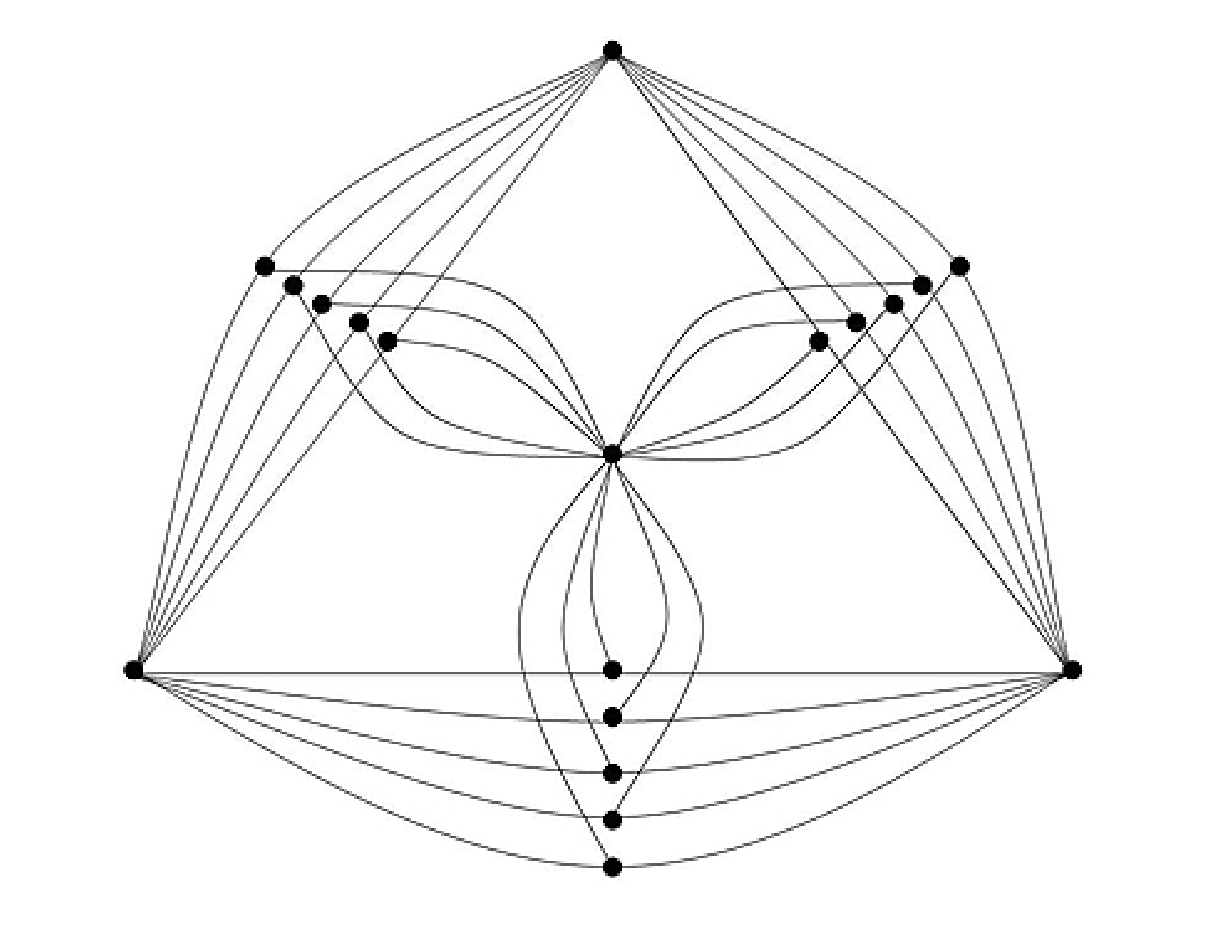
\includegraphics[width=0.6\textwidth]{figures/shannon555.eps}
\end{center}
\end{figure}
\end{frame}


\begin{frame}{Միջակայքային ներկում չունեցող երկկողմանի գրաֆներ}
\begin{itemize}
\item Սեվաստյանով, 1990
\item $\Delta(G)=21$
\end{itemize}

\begin{figure}[h]
\begin{center}
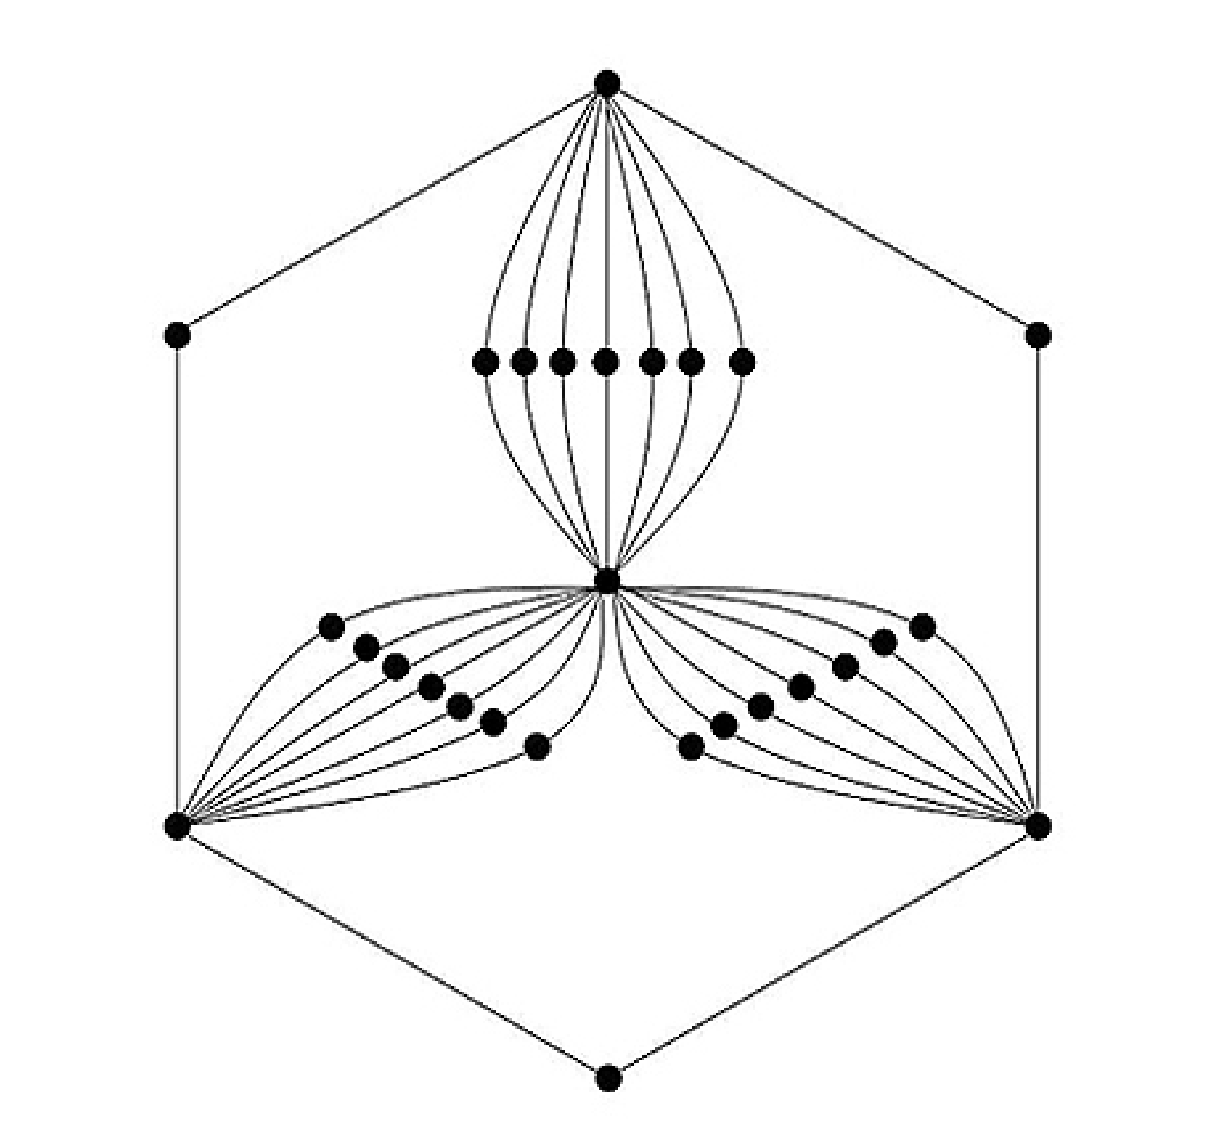
\includegraphics[width=0.6\textwidth]{figures/sevastyanov.eps}
\end{center}
\end{figure}
\end{frame}


\begin{frame}{Միջակայքային ներկում չունեցող երկկողմանի գրաֆներ}
\begin{itemize}
\item Էրդյոշ, 1991
\item $\Delta(G)=13$
\end{itemize}

\begin{figure}[h]
\begin{center}
\includegraphics[width=0.6\textwidth]{figures/erd13.jpg}
\end{center}
\end{figure}
\end{frame}

\begin{frame}[shrink]{Միջակայքային ներկում չունեցող երկկողմանի գրաֆներ}

Ջենսենը և Տոֆտը Graph Coloring Problems (1995) գրքում առաջարկել են հետևյալ խնդիրը.
\begin{problem}
Գոյություն ունի՞ $G$ երկկողմանի գրաֆ, որի համար 
\begin{center}
$4\leq \Delta(G)\leq 12$ և
$G\notin \mathfrak{N}$:
\end{center}
\end{problem}

\pause

Աշխատանքում կառուցվել են միջակայքային ներկում չունեցող երկկողմանի գրաֆների չորս ընտանիքներ.
\begin{enumerate}
    \item Շեննոնի գրաֆների միջոցով կառուցվող հակաօրինակներ
    \item Վերջավոր պրոյեկտիվ երկրաչափություններով հակաօրինակներ
    \item Ծառերի միջոցով կառուցվող հակաօրինակներ
    \item Գրաֆների ենթատրոհումներով կառուցվող հակաօրինակներ
\end{enumerate}
\end{frame}

\begin{frame}{Գրաֆների ենթատրոհումներ}
\begin{itemize}
\item $G$ գրաֆի $S(G)$ ենթատրոհումը ստացվում է $G$-ից՝ յուրաքանչյուր կող մեկ անգամ տրոհելով:
\end{itemize}

\begin{theorem}[Կոստոչկա, 1995; Քամալյան, Միրումյան, 1997; Հանսոն, Լոտեն, Տոֆտ, 1998]
Եթե $G$-ն համասեռ գրաֆ է, ապա $S(G)\in \mathfrak{N}$: 
\end{theorem}
\begin{remark}[3.3.13]
Եթե $G$-ն երկկողմանի գրաֆ է և $G \in \mathfrak{N}$, ապա $S(G)\in \mathfrak{N}$: 
\end{remark}
\pause
\begin{hypothesis}[Պետրոսյան, Խաչատրյան, 2011]
Եթե $G\in \mathfrak{N}$, ապա $S(G)\in \mathfrak{N}$:
\end{hypothesis}

Այս հիպոթեզը հաստատվել է Պյատկինի կողմից (2015):
\end{frame}

\begin{frame}{Գրաֆների ենթատրոհումներով կառուցվող հակաօրինակներ}
\begin{itemize}
\item $G$ գրաֆի $S(G)$ ենթատրոհումը ստացվում է $G$-ից՝ յուրաքանչյուր կող մեկ անգամ տրոհելով:
\item $\widehat{G}$ գրաֆը ստացվում է $S(G)$-ից՝ միացնելով տրոհումից առաջացած գագաթները մի նոր գագաթի:
\end{itemize}
\begin{theorem}[3.3.14]
Եթե $G$-ն կապացված գրաֆ է, և
\begin{center}
$\vert E(G)\vert
> 1+ {\max\limits_{P\in \mathbf{P}}}{\sum\limits_{v\in
V(P)}}\ \left(d_{\widehat{G}}(v)-1\right)$,
\end{center}
որտեղ $\mathbf{P}$-ն $S(G)$-ում տրոհումից առաջացած գագաթները միացնող ամենակարճ շղթաների բազմությունն է, ապա $\widehat{G}\notin \mathfrak{N}$:
\end{theorem}


\end{frame}

\begin{frame}{Միջակայքային ներկում չունեցող երկկողմանի գրաֆներ}
\begin{itemize}
	\item $\Delta(\widehat{K}_{3,4})=12$, $|V(\widehat{K}_{3,4})|=20$
\end{itemize}

\begin{figure}[h]
\begin{center}
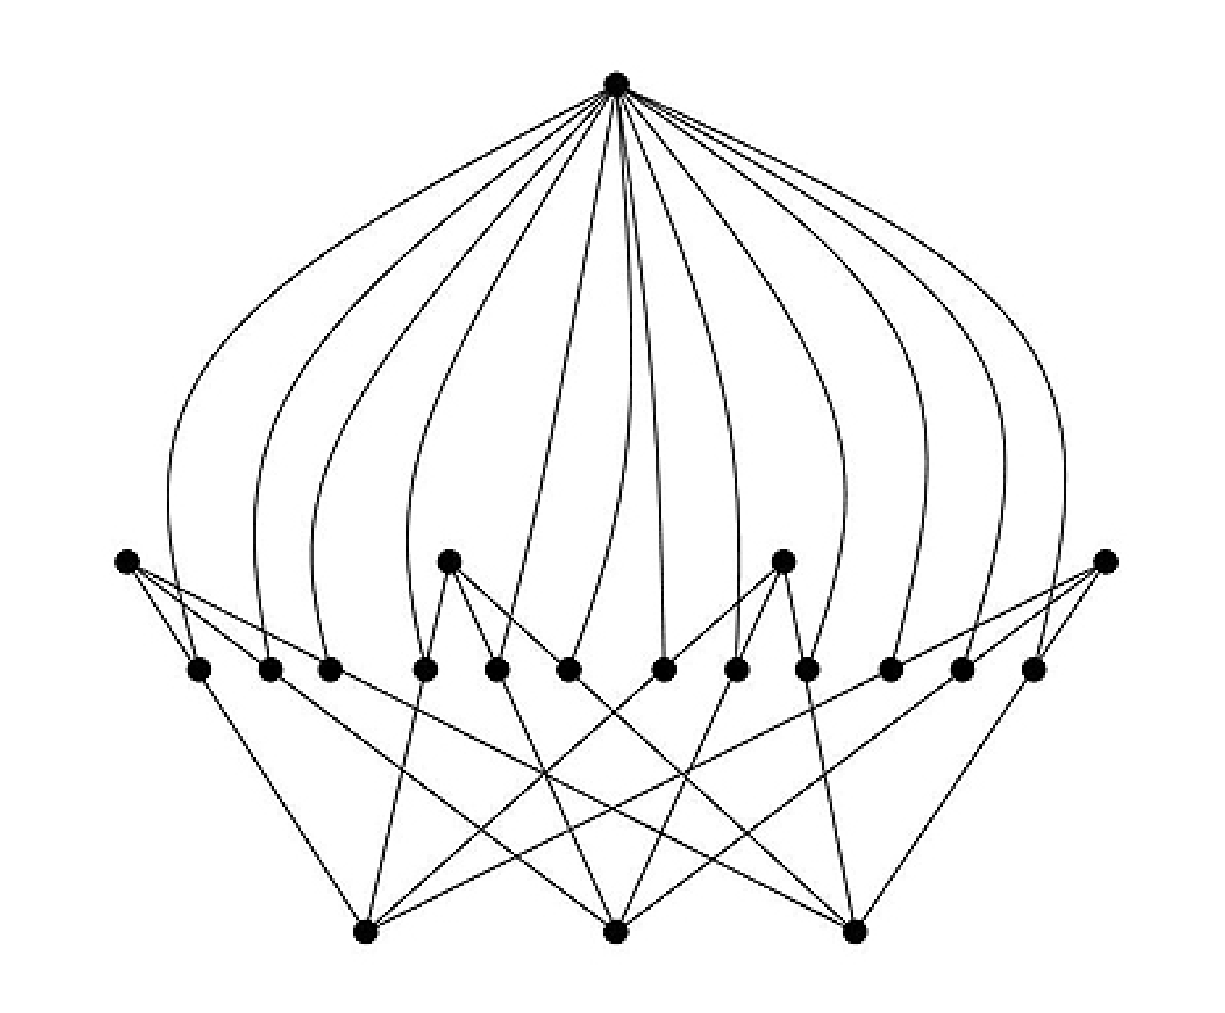
\includegraphics[width=0.5\textwidth]{figures/subdivisionK34.eps}
\end{center}
\end{figure}
\end{frame}


\begin{frame}{Միջակայքային ներկում չունեցող երկկողմանի գրաֆներ}
\begin{itemize}
	\item $\Delta(\widehat{K}_{2,2,2})=12$, $|V(\widehat{K}_{2,2,2})|=19$
\end{itemize}

\begin{figure}[h]
\begin{center}
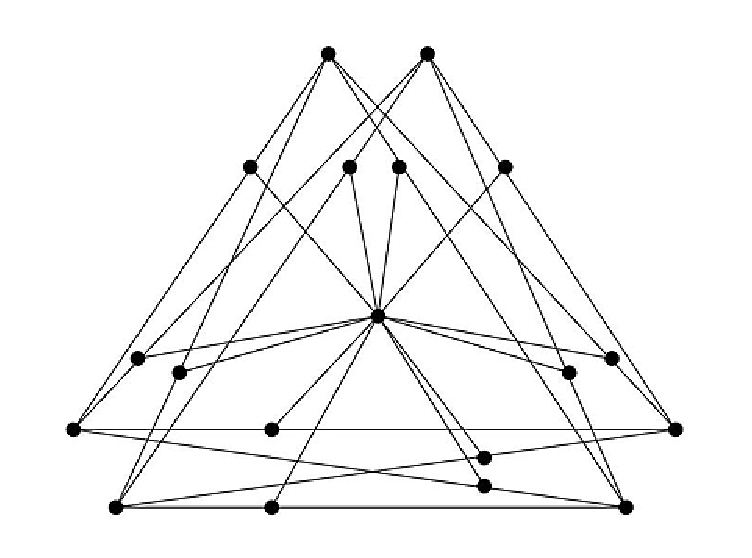
\includegraphics[width=0.5\textwidth]{figures/K222.eps}
\end{center}
\end{figure}
\end{frame}

\begin{frame}{Միջակայքային ներկում չունեցող երկկողմանի գրաֆներ}
\begin{itemize}
	\item $\Delta(\widehat{K}_{3,4}^{\prime})=11$, $|V(\widehat{K}_{3,4}^{\prime})|=20$
\end{itemize}

\begin{figure}[h]
\begin{center}
\includegraphics[width=0.5\textwidth]{figures/K34-prime.jpg}
\end{center}
\end{figure}
\end{frame}





\subsection {Փոքրաթիվ գագաթներով երկկողմանի գրաֆների միջակայքային ներկումներ}

\begin{frame}[shrink]{Միջակայքային ներկում չունեցող երկկողմանի գրաֆներ}

\begin{itemize}
\item (Գիառո, 1999) Բոլոր երկկողմանի գրաֆները, որոնք ունեն առավելագույնը $14$ գագաթ, միջակայքային ներկելի են:
\end{itemize}

\begin{theorem}[3.4.4]
Բոլոր երկկողմանի գրաֆները, որոնք ունեն $15$ կամ $16$ գագաթ, միջակայքային ներկելի են:
\end{theorem}
\begin{table}[t]
\begin{center}
\begin{tabular}{|c|r|r|}
\hline
$|V(G)|$ & Գրաֆների քանակ & Ներկված գրաֆների քանակ \\
\hline
14 & 33 985 853 &  \\
\hline
15 & 611 846 940 & 288 643 868 \\
\hline
16 & 14 864 650 924 & 12 322 367 816 \\
\hline
17 & 488 222 721 992 &  \\
\hline
\end{tabular}
\end{center}
\end{table}

\end{frame}



\subsection{Միջակայքային ներկում չունեցող երկկողմանի մուլտիգրաֆներ}
\begin{frame}{Միջակայքային ներկում չունեցող երկկողմանի մուլտիգրաֆներ}
\begin{theorem}[3.5.3]
Եթե $G$-ն կապակցված երկկողմանի մուլտիգրաֆ է, ընդ որում $\vert V(G)\vert\leq 4$, ապա $G\in \mathfrak{N}$: Իսկ ցանկացած $n \geq 5$ թվի համար գոյություն ունի $G$ կապակցված երկկողմանի մուլտիգրաֆ, որի համար $G\notin \mathfrak{N}$ և $|V(G)|=n$:
\end{theorem}

\begin{figure}[h]
\begin{center}
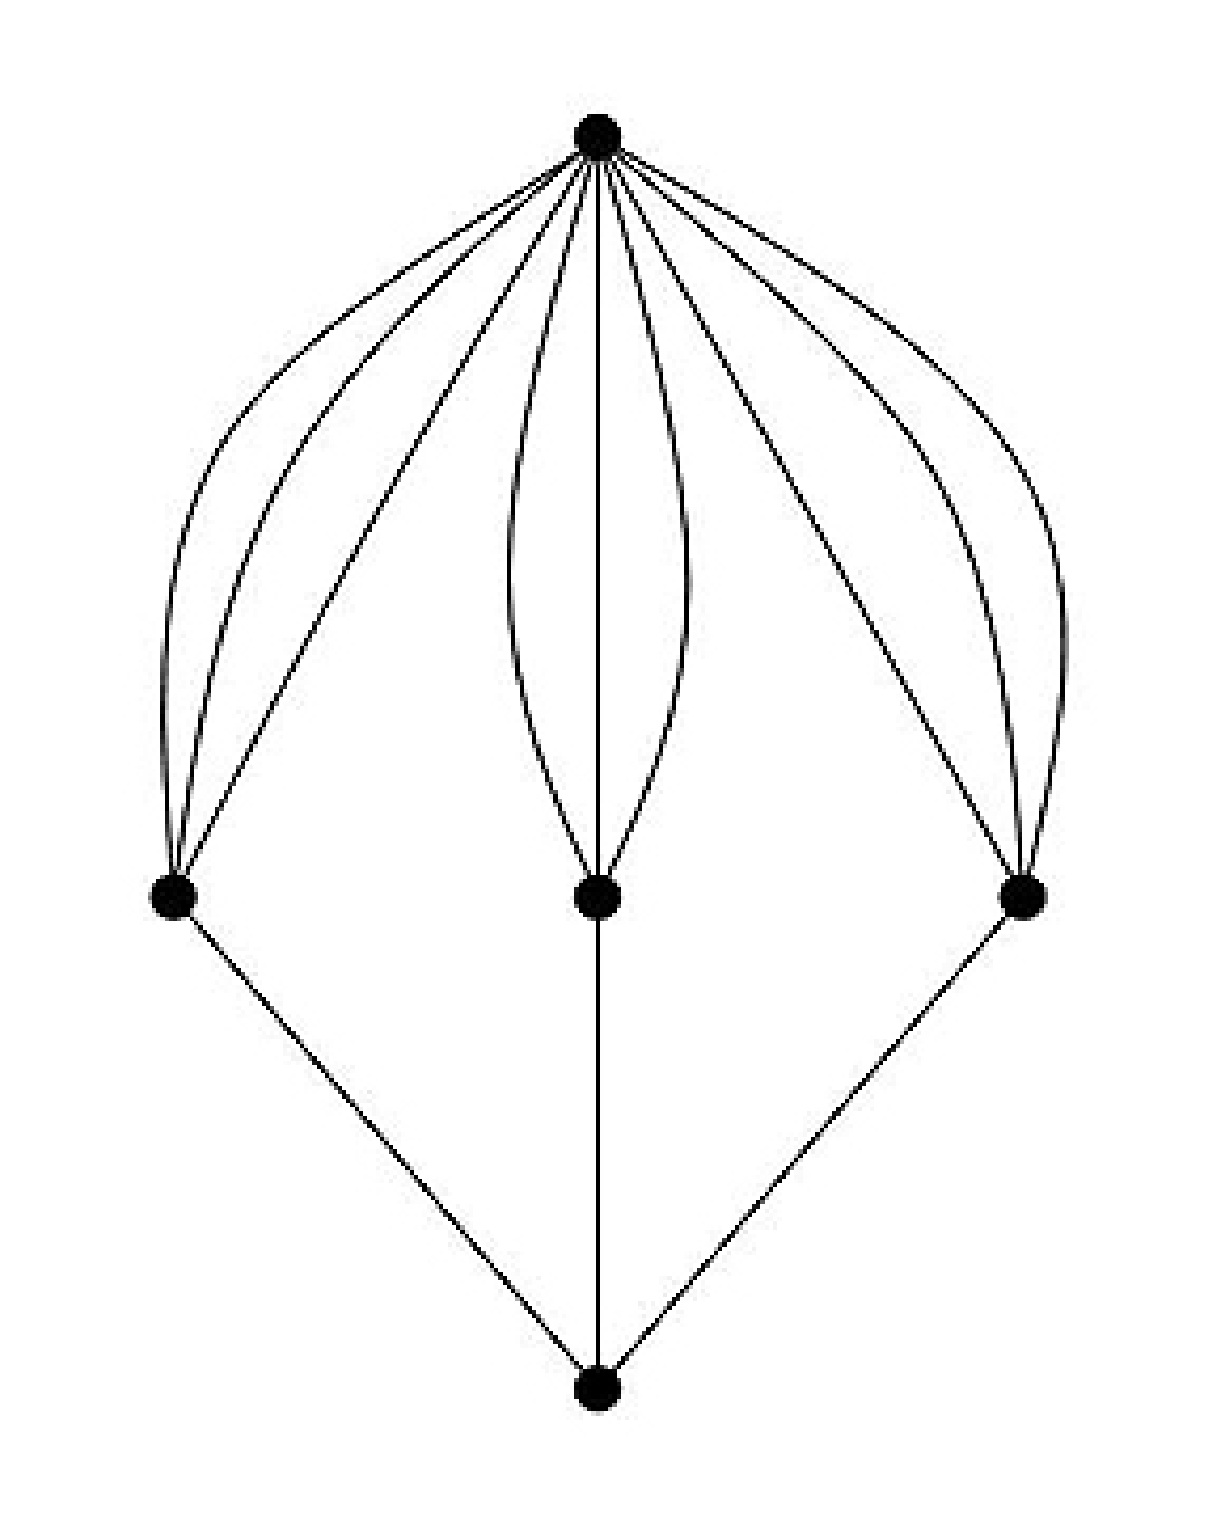
\includegraphics[width=0.25\textwidth]{figures/parachute.eps}
\end{center}
\end{figure}
\end{frame}

\begin{frame}{Միջակայքային ներկում չունեցող երկկողմանի մուլտիգրաֆներ}


\begin{figure}[h]
\begin{center}
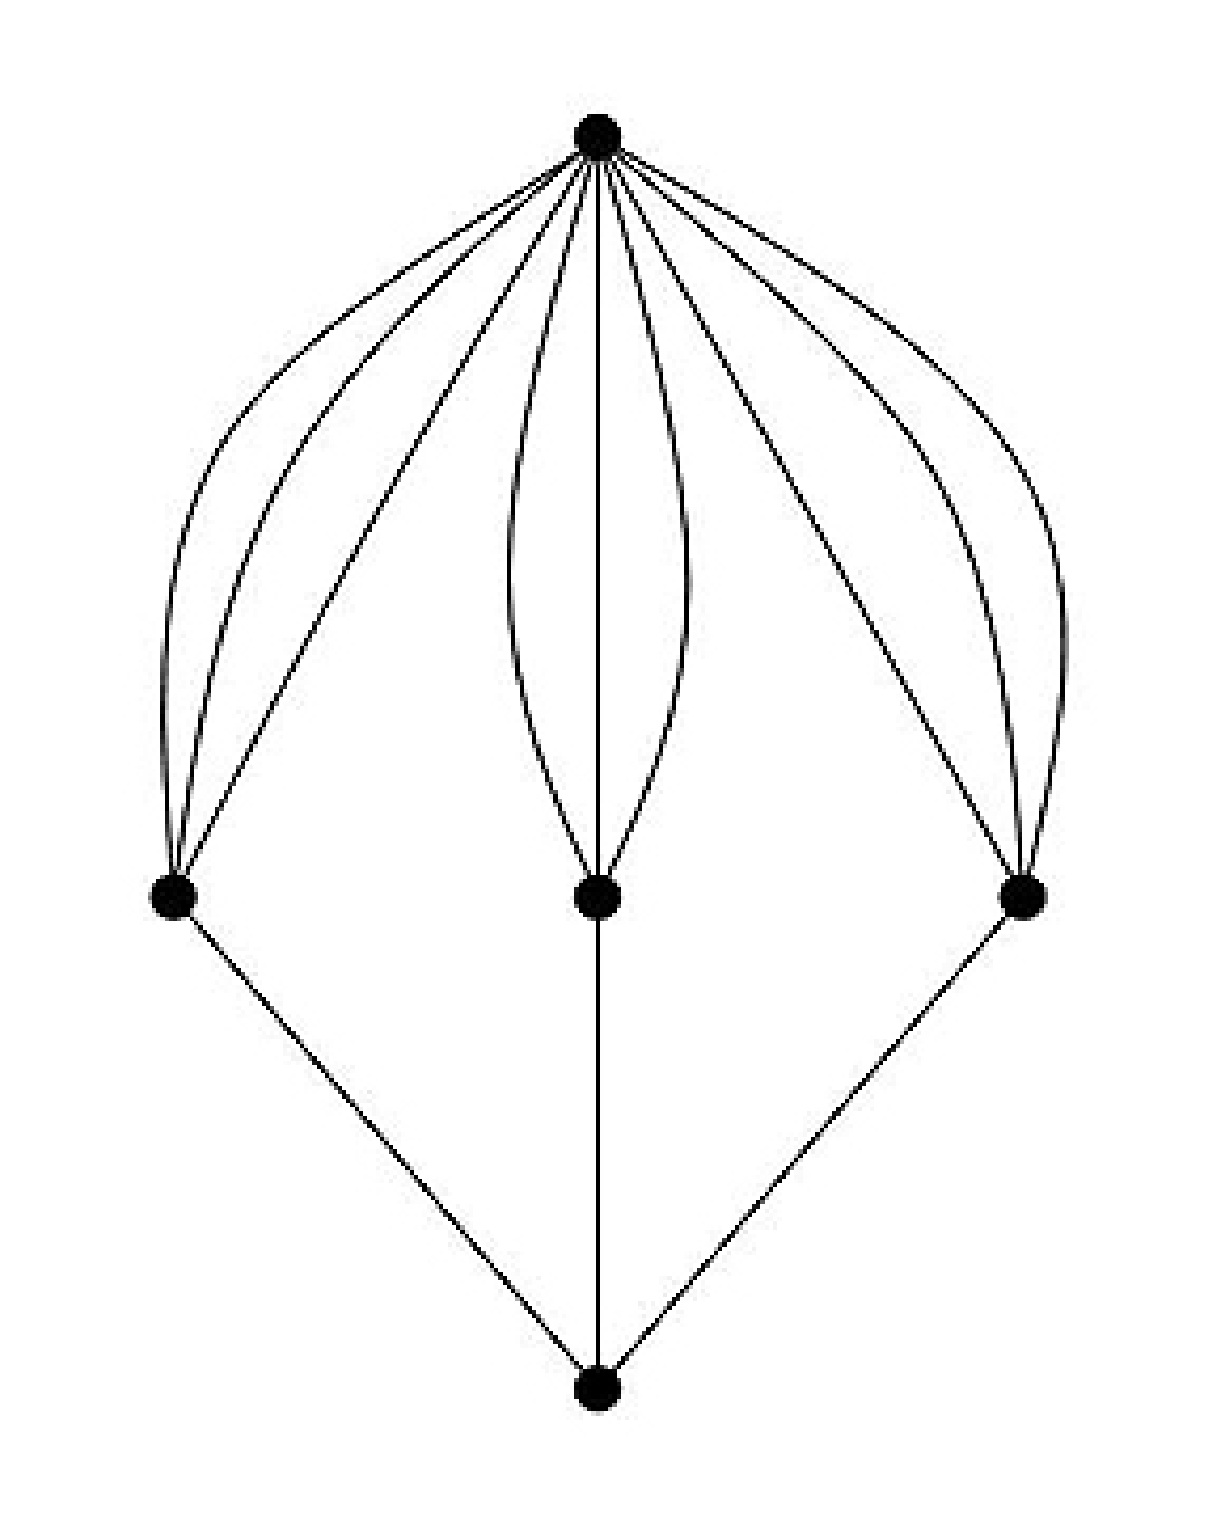
\includegraphics[width=0.25\textwidth]{figures/parachute.eps}
\end{center}
\end{figure}

\begin{theorem}[3.5.4]
Եթե $G$-ն երկկողմանի մուլտիգրաֆ է, որի համար
$\Delta(G)\leq 3$, ապա $G\in \mathfrak{N}$ և $w(G)\leq 4$: Իսկ ցանկացած $\Delta \geq 9$ թվի համար գոյություն ունի $G$ կապակցված երկկողմանի մուլտիգրաֆ, որի համար $G\notin \mathfrak{N}$ և $\Delta(G)=\Delta$:
\end{theorem}

\end{frame}


% \section[Եզրակացություն]*{}
\begin{frame}{Հիմնական արդյունքներն ու հետևությունները}
\begin{enumerate}
\justifying
    \item Միջակայքային ներկումներ ունեցող գրաֆների և մուլտիգրաֆների $w(G)$ և $W(G)$ պարամետրերի, ինչպես նաև միջակայքային ներկում չունեցող գրաֆների $w_{def}(G)$ և $W_{def}(G)$ պարամետրերի համար տրվել են հասանելի գնահատականներ,
    
    \item $K_{2n}$ լրիվ գրաֆների միջակայքային կողային ներկումների և այդ գրաֆների հատուկ տիպի ֆակտորիզացիաների համարժեքության հիման վրա ստացվել են  $W(K_{2n})$ պարամետրի նոր ստորին և վերին գնահատականներ, գտնվել են այդ պարամետրի ճշգրիտ արժեքները $n \leq 12$ արժեքների համար,
    \seti
\end{enumerate}
\end{frame}

\begin{frame}{Հիմնական արդյունքներն ու հետևությունները}{(շարունակություն)}
\begin{enumerate}
    \justifying
    \conti
    \item Ստացվել են լրիվ բազմակողմանի գրաֆների, արտաքին հարթ գրաֆների, ցանցերի, գլանների, տոռերի և Հեմինգի գրաֆների միջակայքային կողային ներկումների գոյության վերաբերյալ արդյունքներ, $w(G)$ և $W(G)$ պարամետրերի գնահատականներ, որոշ դեպքերում՝ նաև ճշգրիտ արժեքներ,

    \item %Ցույց է տրվել գրաֆների միջակայքային ներկելիության կապը այդ գրաֆների մասնակցությամբ դեկարտյան արտադրյալների միջակայքային ներկելիություն հետ, էապես ո
    Ուժեղացվել են համասեռ գրաֆների մասնակցությամբ դեկարտյան արտադրյալների համար $W(G \square H)$ պարամետրի հայտնի գնահատականները, ապացուցվել է երկկողմանի գրաֆների մասնակցությամբ դեկարտյան արտադրյալների մի շարք դասերի միջակայքային ներկելիությունը,
    
    \seti
\end{enumerate}
\end{frame}

\begin{frame}{Հիմնական արդյունքներն ու հետևությունները}{(շարունակություն)}
\begin{enumerate}
    % \fontsize{10pt}{11}\selectfont
    \justifying
    \conti
    \item %Գտնվել են որոշ գրաֆների դեֆիցիտի ճշգրիտ արժեքները, 
    Հաստատվել է Բորովիցկա-Օլշեվսկայի, Դրգաշ-Բուրչարդտի և Հալուշչակի հիպոթեզը, ցույց է տրվել, որ արտաքին հարթ գրաֆները բավարարում են դեֆիցիտի մասին հիպոթեզին, համաձայն որի ցանկացած $G$ գրաֆի համար $def(G) \leq |V(G)|$,

    \item Մասնակի լուծում է տրվել միջակայքային ներկում չունեցող փոքրագույն երկկողմանի գրաֆների մասին Ջենսեն-Տոֆտի խնդրին, կառուցվել են այդպիսի գրաֆների և մուլտիգրաֆների հայտնի փոքրագույն օրինակները, համակարգչային հաշվարկների միջոցով ցույց է տրվել, որ ոչ ավել, քան 16 գագաթ պարունակող բոլոր երկկողմանի գրաֆները ունեն միջակայքային ներկումներ:
    
    \seti
\end{enumerate}
\end{frame}


% \section*{Ատենախոսության թեմայի շրջանակներում հրապարակված աշխատանքները}
\begin{enumerate}
    \itemsep0em 
    \item P.A. Petrosyan, H.H. Khachatrian, Further results on the deficiency of graphs, Discrete Applied Mathematics, 2017, http://dx.doi.org/10.1016/j.dam.2017.04.005.
    \item H.H. Khachatrian, Deficiency of outerplanar graphs, Proceedings of the Yerevan State University. Physical and Mathematical Sciences, 2017, 51 (1), pp. 22-28.
    \item H.H. Khachatrian, P.A. Petrosyan, Interval edge-colorings of complete graphs, Discrete Mathematics 339, 2016, pp. 2249-2262.
    \item P.A. Petrosyan, H.H. Khachatrian, T.G. Mamikonyan, On interval edge-colorings of bipartite graphs, 2015 Computer Science and Information Technologies (CSIT), Yerevan, 2015, pp. 71-76.
    \item H.H. Khachatrian, P.A. Petrosyan, Interval edge-colorings of Hamming graphs, 8th Slovenian Conference on Graph Theory, Kranjska Gora, Slovenia, 2015, p. 134.
    \item P.A. Petrosyan, H.H. Khachatrian, Interval non-edge-colorable bipartite graphs and multigraphs, Journal of Graph Theory 76, Issue 3, 2014, pp. 200-216.
    \item A. Grzesik, H.H. Khachatrian, Interval edge-colorings of $K_{1,m,n}$, Discrete Applied Mathematics 174, 2014, pp. 140-145.
    \item H.H. Khachatrian, P.A. Petrosyan, Interval edge-colorings of complete graphs, 7th Cracow Conference on Graph Theory, Rytro, Poland, 2014, pp. 35-36.
    \item A. Grzesik, H.H. Khachatrian, P.A. Petrosyan, On interval edge-colorings of complete multipartite graphs, 5th Polish Combinatorial Conference, Bedlewo, Poland, 2014, p. 29.
    \item P.A. Petrosyan, H.H. Khachatrian, H.G. Tananyan, Interval edge-colorings of Cartesian products of graphs I, Discussiones Mathematicae Graph Theory 33(3), 2013, pp. 613-632.
    \item A. Grzesik, H. Khachatrian, On interval edge-colorings of complete tripartite graphs, 9th International Conference on Computer Science and Information Technologies, Revised Selected Papers, Yerevan, 2013, pp. 1-3.
    \item P.A. Petrosyan, H.H. Khachatrian, On a generalization of interval edge colorings of graphs, 15th Workshop on Graph Theory, Colourings, Independence and Domination, Szklarska Poreba, Poland, 2013, p. 44.
    \item P.A. Petrosyan, H.H. Khachatrian, H.G. Tananyan, Interval edge-colorings of Cartesian products of graphs, 14th Workshop on Graph Theory, Colourings, Independence and Domination, Szklarska Poreba, Poland, 2011, p. 44.
    \item P.A. Petrosyan, H.H. Khachatrian, L.E. Yepremyan, H.G. Tananyan, Interval edge-colorings of graph products, Proceedings of the CSIT Conference, Yerevan, 2011, pp. 89-92.
    \item П.А. Петросян, Г.А. Хачатрян, Интервальные реберные раскраски декартовых произведений регулярных графов, Пятая годичная научная конференция РАУ (Сборник научных работ), 2010, стр. 241-248.
\end{enumerate}

% \begin{thebibliography}{99}
% \bibitem{AltinakarCaporossiHertz} H.S. Altinakar, G. Caporossi, A. Hertz, A comparison of integer and constraint programming models for the deficiency problem, Computers and Oper. Res. 68, 2016, pp. 89-96.
\bibitem{AppelHaken1} K. Appel, W. Haken, Every planar map is four colorable, Part I, Discharging, Illinois Journal of Mathematics 21, 1977, pp. 429-490.
\bibitem{AppelHaken2} K. Appel, W. Haken, J. Koch, Every planar map is four colorable, Part II, Reducibility, Illinois Journal of Mathematics 21, 1977, pp. 491-567.
\bibitem{Asratian2000} A.S. Asratian, Some results on an edge coloring problem of Folkman and Fulkerson, Discrete Math. 223, 2000, pp. 13-25.
\bibitem{AsratianKamalian1994} A.S. Asratian, R.R. Kamalian, Investigation on interval edge-colorings of graphs, J. Combin. Theory Ser. B 62, 1994, pp. 34-43. 
\bibitem{AsratianDenleyHaggvist1998} A.S. Asratian., T.M.J. Denley, R. Haggkvist, Bipartite graphs and their applications, Cambridge Tracts in Mathematics, Cambridge University Press, 1998.
\bibitem{AsratianCasselgrenPetrosyan2017} A.S. Asratian, C.J. Casselgren, P.A. Petrosyan, Some results on cyclic interval colorings of graphs, J. Graph Theory, 2017, ընդունված է տպագրության:
\bibitem{AsratianCasselgrenVandenbusscheWest2009} A.S. Asratian, C.J. Casselgren, J. Vandenbussche, D.B. West, Proper path-factors and interval edge-coloring of (3,4)-biregular bigraphs, J. Graph Theory 61, 2009, pp. 88-97.
\bibitem{Axenovich2002} M.A. Axenovich, On interval colorings of planar graphs, Congressus Numerantium 159, 2002, pp. 77-94.
\bibitem{BehzadMahmoodian1969} M. Behzad, E.S. Mahmoodian, On topological invariants of the product of graphs, Canad. Math. Bull., 12, 1969, pp. 157-166.
\bibitem{BeinekeWilson} L.W. Beineke, R.J. Wilson, On the edge-chromatic number of a graph, Discrete Math. 5, 1973, pp. 15-20.
\bibitem{Berge1958} C. Berge, Theorie des Graphes et ses Applications, Dunod, Paris, 1958.
\bibitem{BorowieckaDrgas2016} M. Borowiecka-Olszewska, E. Drgas-Burchardt, The deficiency of all generalized Hertz graphs and minimal consecutively non-colourable graphs in this class. Discrete Math. 339, 2016, pp. 1892-1908.
\bibitem{B-OD-BHal} M. Borowiecka-Olszewska, E. Drgas-Burchardt, M. Ha\l uszczak, On the structure and deficiency of $k$-trees with bounded degree, Discrete Appl. Math. 201, 2016, pp. 24-37.
\bibitem{BouchardHertzDesaulniers} M. Bouchard, A. Hertz, G. Desaulniers, Lower bounds and a tabu search algorithm for the minimum deficiency problem, J. Comb. Optim. 17, 2009, pp. 168-191.
\bibitem{CasselgrenPetrosyanToft2017} C.J. Casselgren, P.A. Petrosyan, B. Toft, On interval and cyclic interval edge colorings of (3,5)-biregular graphs, Discrete Mathematics, 2017, ընդունված է տպագրության:
\bibitem{CarlJToft} C.J. Casselgren, B. Toft, On interval edge colorings of biregular bipartite graphs with small vertex degrees, J. Graph Theory 80, 2015, pp. 83-97.% http://dx.doi.org/10.1002/jgt.21841
\bibitem{CrowdProcess} CrowdProcess distributed computing platform [առցանց].  \url{http://www.crowdprocess.com/}
\bibitem{DeWerra1971Balanced} D. de Werra, Balanced schedules, INFOR. N9, 1971, pp. 230-237.
\bibitem{DeWerra1971} D. de Werra, Investigations on an edge coloring problem, Discrete Math. 1, 1971, pp. 167-179.
\bibitem{DeWerraSolot1991} D. de Werra, Ph. Solot, Compact cylindrical chromatic scheduling, SIAM J. Discrete Math. 4, 1991, pp. 528-534.
\bibitem{DulmageMendelsohn} A.L. Dulmage, N.S. Mendelsohn, Some graphical properties of matrices with nonnegative entries, Acquat. Math., 2, 1969, pp. 150-162.
\bibitem{ErdosRubinTaylor} P. Erdős, A.L. Rubin, H. Taylor, Choosability in graphs, Proc. West Coast Conf. on Combinatorics, Graph Theory and Computing, Congr. Numer. 26, 1979, pp. 125-157.
\bibitem{EvenItaiShamir} S. Even, A. Itai, A. Shamir, On the complexity of timetable and multicommodity flow problems, SIAM J. Comput. 5 (4), 1976, pp. 691-703.
\bibitem{FengHuang2007} Y. Feng, Q. Huang, Consecutive edge-coloring of the generalized $\theta$-graph, Discrete Appl. Math. 155, 2007, pp. 2321-2327. %doi:10.1016/j.dam.2007.06.010
\bibitem{Fiorini1975} S. Fiorini, On the chromatic index of outerplanar graphs, J. Combin. Theory Ser. B 18, 1975, pp. 35-38. %doi:10.1016/0095-8956(75)90060-X
\bibitem{FolkmanFulkerson} J. Folkman, D.R. Fulkerson, Edge colourings in bipartite graphs, in Combinatorial  Mathematics and its Applications, University of North Carolina Press, Chapel Hill, 1969, pp. 561-577.
\bibitem{Giaro1997} K. Giaro, The complexity of consecutive $\Delta $-coloring of bipartite graphs: $4$ is easy, $5$ is hard, Ars Combin. 47, 1997, pp. 287-298.
\bibitem{Giaro1999} K. Giaro, Compact task scheduling on dedicated processors with no waiting periods, PhD thesis, Technical University of Gdansk, EIT faculty, Gdansk, 1999 (լեհերեն).
\bibitem{GiaroKubale1997}	K. Giaro, M. Kubale, Consecutive edge-colorings of complete and incomplete Cartesian products of graphs, Cong, Num. 128, 1997, pp. 143-149. 
\bibitem{GiaroKubale2004}	K. Giaro, M. Kubale, Compact scheduling of zero-one time operations in multi-stage systems, Discrete Appl. Math. 145, 2004, pp. 95-103.
\bibitem{GiaroKubaleMalafiejski1999} K. Giaro, M. Kubale, M. Malafiejski, On the deficiency of bipartite graphs, Discrete Appl. Math. 94, 1999, pp. 193-203.
\bibitem{GiaroKubaleMalafiejski2001} K. Giaro, M. Kubale, M. Malafiejski, Consecutive colorings of the edges of general graphs, Discrete Math. 236, 2001, pp. 131-143.
\bibitem{HansonLoten} D. Hanson, C.O.M. Loten, A lower bound for interval colouring bi-regular bipartite graphs, Bulletin of the ICA 18, 1996, pp. 69-74.
\bibitem{HansonLotenToft1998}	D. Hanson, C.O.M. Loten, B. Toft, On interval colorings of bi-regular bipartite graphs, Ars Combin. 50, 1998, pp. 23-32.
\bibitem{Harary1969} F. Harary, Graph Theory, Addison-Wesley, Reading, MA, 1969. 
\bibitem{Harary1974} H.J. Fleischner, D.P. Geller, F. Harary, Outerplanar graphs and weak duals, J. Indian Math. Soc. 38, 1974, pp. 215-219.
\bibitem{Hansen1992} H.M. Hansen, Scheduling with minimum waiting periods, Master's Thesis, Odense University, Odense, Denmark, 1992 (դանիերեն).
\bibitem{JensenToft1995} T.R. Jensen, B. Toft, Graph coloring problems, Wiley Interscience Series in Discrete Mathematics and Optimization, 1995.
\bibitem{KamalianPetrosyan2012}	R.R. Kamalian, P.A. Petrosyan, A note on upper bounds for the maximum span in interval edge-colorings of graphs, Discrete Math. 312, 2012, pp. 1393-1399.
\bibitem{Konig1916} D. König, \textit{Uber Graphen und ihre Anwendung auf Determinantentheorie und Mengenlehre}, Math. Ann. 77, 1916, pp. 453-465.
\bibitem{Kubale2004} M. Kubale, Graph Colorings, American Mathematical Society, 2004.
\bibitem{KubickaSum} E. Kubicka, The chromatic sum of a graph, PhD Thesis, Western Michigan University, 1989.
\bibitem{McKay} B.D. McKay, A. Piperno, Practical Graph Isomorphism, II, J Symbolic Computation, vol. 60, 2014, pp. 94-112. %http://dx.doi.org/10.1016/j.jsc.2013.09.003
\bibitem{Petrosyan2010}	P.A. Petrosyan, Interval edge-colorings of complete graphs and n-dimensional cubes, Discrete Math. 310, 2010, pp. 1580-1587.
\bibitem{Petrosyan2011}	P.A. Petrosyan, Interval edge colorings of some products of graphs, Discuss. Math. Graph Theory 31(2), 2011, pp. 357-373.
\bibitem{Petrosyan2012}	P.A. Petrosyan, Interval colorings of complete balanced multipartite graphs, arxiv:1211.5311, 2012.
\bibitem{Petrosyan2013}	P.A. Petrosyan, On Interval Non-Edge-Colorable Eulerian Multigraphs, arxiv:1311.2210, 2013.
\bibitem{Petrosyan2013Outerplanar} P.A. Petrosyan, On Interval Edge-Colorings of Outerplanar Graphs, Ars Combin. 132, 2017, pp. 127-135.
\bibitem{PetrosyanArakelyan2007} P.A. Petrosyan, H.Z. Arakelyan, On a generalization of interval edge colorings of graphs. Transactions of IPIA of NAS RA, Math. Probl. of Comp. Sci. 29, 2007, pp. 26-32.
\bibitem{PetrosyanKarapetyan2007} P.A. Petrosyan, G.H. Karapetyan, Lower bounds for the greatest possible number of colors in interval edge colorings of bipartite cylinders and bipartite tori, Proceedings of the CSIT Conference, Yerevan, 2007, pp. 86-88.
\bibitem{PetrosyanKhachatrianCID2013} P.A. Petrosyan, H.H. Khachatrian, On a generalization of interval edge-colorings of graphs, 15th Workshop on Graph Theory, Colourings, Independence and Domination, Szklarska Poreba, Poland, 2013, p. 44.
\bibitem{PetrosyanKhachatrian2014} P.A. Petrosyan, H.H. Khachatrian, Interval non-edge-colorable bipartite graphs and multigraphs, J. Graph Theory 76, 2014, pp. 200-216.
\bibitem{PetrosyanKhachatrianTananyan2011}	P.A. Petrosyan, H.H. Khachatrian, H.G. Tananyan, Interval edge-colorings of Cartesian products of graphs, CID abstracts, 2011, p.44. http://www.cid.uz.zgora.pl/2011/files/AbstractsPdf/Khachatrian.pdf
\bibitem{PetrosyanKhachatrianTananyan2013}	P.A. Petrosyan, H.H. Khachatrian, H.G. Tananyan, Interval edge-colorings of Cartesian products of graphs I, Discuss. Math. Graph Theory 33(3), 2013, pp. 613-632.
\bibitem{PetrosyanKhachatrianYepremyanTananyan2011} P.A. Petrosyan, H.H. Khachatrian, L.E. Yepremyan, H.G. Tananyan, Interval edge-colorings of graph products, Proceedings of the CSIT Conference, 2011, pp. 89-92.
\bibitem{PetrosyanMkhitaryan} P.A. Petrosyan, S.T. Mkhitaryan, Interval cyclic edge-colorings of graphs, Discrete Math. 339, 2016, pp. 1848-1860.
\bibitem{Pyatkin2004}	A.V. Pyatkin, Interval coloring of (3,4)-biregular bipartite graphs having large cubic subgraphs, J. Graph Theory 47, 2004, pp. 122-128.
\bibitem{Sabidussi1960} G. Sabidussi, Graph multiplication, Math. Z. 72, 1960, pp. 446-457.
\bibitem{Shannon1949} C.E. Shannon, A theorem on colouring the lines of a network, J. Math. Phys. 28, 1949, pp. 148-151.
\bibitem{Schwartz2006} A. Schwartz, The deficiency of a regular graph. Discrete Math. 306, 2006, pp. 1947-1954.
\bibitem{Stiebitz2012} M. Stiebitz, D. Scheide, B. Toft, L.M. Favrholdt, Graph Edge Coloring: Vizing's Theorem and Goldberg's Conjecture, Wiley Interscience Series in Discrete Mathematics and Optimization, 2012. 
\bibitem{SupowitSum} K.J. Supowit, Finding a maximum planar subset of nets in a channel, IEEE Trans. Comput. Aided Design CAD 6(1), 1987, pp. 93-94.
\bibitem{TepanyanPetrosyan} H.H. Tepanyan, P.A. Petrosyan, Interval edge-colorings of composition of graphs, Discrete Appl. Math. 217, 2017, pp. 368-374.
\bibitem{West1996}	D.B. West, Introduction to Graph Theory, Prentice-Hall, New Jersey, 1996.
\bibitem{YangLi2011}	F. Yang, X. Li, Interval coloring of (3,4)-biregular bigraphs having two (2,3)-biregular bipartite subgraphs, Applied Math. Letters 24, 2011, pp. 1574-1577. 
\bibitem{AsratianKamalian1987} А.С. Асратян, Р.Р. Камалян, Интервальные раскраски ребер мультиграфа, Прикладная математика, вып. 5, 1987, стр. 25-34.
\bibitem{Vizing1963} В.Г. Визинг, Декартовое произведение графов, Вычис. Системы 9, 1963, стр. 30-43. 
\bibitem{Vizing1965} В.Г. Визинг, Хроматический класс мультиграфов, Кибернетика 3, 1965, стр. 29-39.
\bibitem{Vizing1965critical} В.Г. Визинг, Критические графы с данным хроматическим классом, Дискретный анализ 5, 1965, стр. 9-17.
\bibitem{VizingVertex} В.Г. Визинг, Раскраска вершин графа в предписанные цвета, Методы дискретного анализа 29, 1976, стр. 3-10.
\bibitem{Kamalian1989}	Р.Р. Камалян, Интервальные раскраски полных двудольных графов и деревьев, Препринт ВЦ АН Арм. ССР и ЕГУ, Ереван, 1989, 11 стр. 
\bibitem{Kamalian1990}	Р.Р. Камалян, Интервальные реберные раскраски графов, канд. дисс., Новосибирск, 1990.
\bibitem{Kamalian2010}	Р.Р. Камалян, Об одном классе планарных двудольных графов, не имеющих интервальной реберной раскраски, Գիտական հոդվածների ժողովածու, ԵՊՀ Իջևանի մասնաճյուղ, 2010, стр. 149-151
\bibitem{KamalianMirumyan1997}	Р.Р. Камалян, А.Н. Мирумян, Интервальные реберные раскраски двудольных графов одного класса, Доклады НАН РА, том 97, N 4, 1997, стр. 3-5. 
\bibitem{PetrosyanKhachatrian2010} П.А. Петросян, Г.А. Хачатрян, Интервальные реберные раскраски декартовых произведений регулярных графов, Пятая годичная научная конференция РАУ, Сборник научных работ, 2010, стр. 241-248.
\bibitem{Pyatkin2015} А.В. Пяткин, Об интервальной (1,1)-раскраске инциденторов интервально раскрашиваемых графов, Дискретн. анализ и исслед. опер. 22:2, 2015, стр. 63-72.
\bibitem{Sevastyanov1990} С.В. Севастьянов, Об интервальной раскрашиваемости ребер двудольного графа, Методы дискретного анализа в решении экстремальных задач, вып. 50, 1990, стр. 61-72.
\bibitem{Yepremyan2011}	Լ. Եփրեմյան, Գրաֆների արտադրյալների միջակայքային ներկումների մասին, մագիստրոսական թեզ, Երևանի Պետական Համալսարան, 2011, 56 էջ:
\bibitem{Kchoyan2010} Ա. Խչոյան, Ենթախորանարդ գրաֆների և մուլտիգրաֆների միջակայքային կողային ներկումներ, ավարտական աշխատանք, Երևանի Պետական Համալսարան, 2010, 30 էջ:
\bibitem{MamikonyanGithub} Տ. Մամիկոնյան, graphonline բաշխված համակարգ [առցանց]. \url{https://github.com/sarahmiracle/graphonline}
\bibitem{PMK2015} Պ.Ա. Պետրոսյան, Վ.Վ. Մկրտչյան, Ռ.Ռ. Քամալյան, Գրաֆների տեսություն, ուսումն. ձեռն., Երևան, ԵՊՀ հրատ., 2015:
% \end{thebibliography}

\end{document}